\documentclass[11pt]{article}
\usepackage[a4paper,margin=2.2cm]{geometry}
\usepackage{amsmath,amssymb}
\usepackage{booktabs}
\usepackage{xcolor}
\usepackage{hyperref}
\usepackage{enumitem}
\usepackage{graphicx}
\usepackage{caption}
\usepackage{tikz}
\usetikzlibrary{shapes.geometric, arrows.meta, positioning, fit}
\usepackage{fancyhdr}
\usepackage{longtable}
\usepackage{float}

\newcommand{\meaningpar}[1]{\par\noindent\textit{Meaning.} #1}
\newcommand{\good}[1]{\textcolor{green!45!black}{#1}}
\newcommand{\bad}[1]{\textcolor{red!55!black}{#1}}

\pagestyle{fancy}
\fancyhf{}
\fancyhead[L]{\small MetaFVG Spearman Mean-Reversion Gate --- Research Report}
\fancyhead[R]{\small\thepage}
\renewcommand{\headrulewidth}{0.3pt}

\title{\vspace{-1.5em}MetaFVG: A Fair Value Gap Mean-Reversion Strategy\\[4pt]
\large Signal Construction, Risk Management, and Portfolio-Level Backtest Results}
\author{Research notes --- \texttt{metalib/research/}}
\date{Reference setup: HTF = 4h, LTF = M15, equal-weight 14-instrument portfolio, fixed 2\% notional sizing\\
5-year backtest window ending July 2026}

\begin{document}
\maketitle
\vspace{-1em}

\begin{abstract}
\noindent MetaFVG is a Fair Value Gap (FVG) strategy that trades higher-timeframe (HTF) liquidity
imbalances confirmed by lower-timeframe (LTF) momentum. This report documents the
\emph{mean-reversion} variant: a rolling Spearman rank-correlation gate on HTF closes that, when its
sign \emph{disagrees} with a detected FVG zone's own directional bias, redirects the trade (both the
LTF confirmation and the trade parameters) to follow the disagreeing signal instead of the zone. The
strategy is backtested across a 14-instrument universe assembled to be diversified by fundamental
macro driver (7 FX Majors, 4 equity indices from different central banks, 3 additional FX minors),
blended with equal weights. Over a 5-year window the equal-weight portfolio achieves a Sharpe ratio
of $0.518$ (Sortino $0.817$, Calmar $0.343$) with realized average pairwise correlation between
instruments' \emph{traded P\&L} of only $0.0156$ --- an order of magnitude below the underlying
instruments' raw price-return correlation. A companion study testing four correlation-aware,
non-equal-weight allocation schemes (inverse-volatility, equal risk contribution, hierarchical risk
parity, inverse average-correlation) found none improved on equal weighting's Sharpe; the results are
summarized in \S\ref{sec:weighting} and detailed in full in \texttt{weighting\_schemes/comparison\_summary.pdf}.
\end{abstract}

\tableofcontents

\section{Introduction}
Fair Value Gaps are three-candle price imbalances left behind by impulsive moves: a gap between the
high (or low) of one candle and the low (or high) of a candle two bars later that the middle candle's
range never covers. The working hypothesis behind MetaFVG is that price revisiting such a gap on a
higher timeframe is a meaningful liquidity/inefficiency event worth conditioning a trade on, provided
a lower-timeframe momentum pattern confirms the move is actually underway at entry time.

The variant documented here layers a second, independent signal on top of the raw FVG zone: a rolling
Spearman rank-correlation statistic computed on HTF closes. Rather than using this purely as an
agree/reject filter on the zone's own direction, the \emph{mean-reversion} configuration takes the
gate's sign as authoritative whenever it disagrees with the zone: the trade, its LTF confirmation, and
its risk parameters all pivot to follow the gate, not the zone. This report documents the full signal
pipeline (\S\ref{sec:methodology}--\ref{sec:diagram}), the instrument universe and the rationale for
its construction (\S\ref{sec:universe}), the backtest methodology (\S\ref{sec:data}), and portfolio-
and instrument-level results (\S\ref{sec:results}--\ref{sec:persymbol}), before a parameter sensitivity
sweep (\S\ref{sec:sensitivity}), a follow-up test of the outperforming configurations it surfaced
(\S\ref{sec:outperforming}), a correlation-aware position-sizing study (\S\ref{sec:weighting}), and
closing with limitations (\S\ref{sec:limitations}).

\section{Strategy Methodology}
\label{sec:methodology}

\subsection{HTF Fair Value Gap Detection}
On the HTF (4h) series, a bullish FVG is registered at bar $i$ when
$\mathrm{low}_{i+1} > \mathrm{high}_{i-1}$, with zone bounds $[\mathrm{high}_{i-1},\,\mathrm{low}_{i+1}]$;
a bearish FVG is the mirror condition, $\mathrm{high}_{i+1} < \mathrm{low}_{i-1}$, zone
$[\mathrm{high}_{i+1},\,\mathrm{low}_{i-1}]$. The HTF series itself is produced by a \emph{causal}
resample of the underlying LTF data (\texttt{label=`right'}, \texttt{closed=`left'}): a 4h bucket's
close is only attributed to a bar once the full 4 hours have elapsed, which rules out a bucket's own
future close leaking into zone detection before that bar has actually finished forming.

\subsection{Zone Filtering}
Raw FVG zones are filtered on two criteria before becoming tradeable:
\begin{itemize}[nosep]
  \item \textbf{Fill-\% threshold}: price must retrace into the zone by at least a configured
  fraction of its height (\texttt{htf\_fill\_pct}) before the zone is considered ``live.''
  \item \textbf{Max crossing count}: a zone that has been crossed by price more than
  \texttt{max\_htf\_number\_crossings} times is treated as exhausted and dropped.
\end{itemize}
The current price is then checked against the surviving zone set on both sides (bullish and bearish);
if it sits inside a filtered zone, that zone's polarity implies a candidate direction
$d\in\{+1,-1\}$ ($+1$ bullish, $-1$ bearish).

\subsection{Spearman Mean-Reversion Gate}
A rolling Spearman rank correlation is computed on the trailing $w$-bar (default $w=20$) window of
HTF closes:
\[
\rho_t = 1 - \frac{6\sum_t d_t^2}{w(w^2-1)}, \qquad d_t = \operatorname{rank}(c_t) - t
\]
\meaningpar{$\operatorname{rank}(c_t)$ is the close price's rank (1st-smallest, \dots, $w$-th-smallest)
within the window; $t$ is already the bar's rank in time. $d_t$ is the gap between ``where this bar
ranks by price'' and ``where it ranks by time.'' $\rho_t \in [-1,1]$ summarizes that agreement:
$+1$ means price rank and time rank move together perfectly (a monotonic uptrend, any shape), $-1$
means perfectly monotonic down, $0$ means no consistent ordering.}

Let $d$ be the candidate direction implied by the HTF zone (as above). Define the \textbf{target
direction} under the mean-reversion configuration as
\[
d_{\text{target}} = \begin{cases} d & \text{trend-following configuration} \\ -d &
\text{mean-reversion configuration (\texttt{invert\_direction=True})} \end{cases}
\]
The gate accepts a signal iff
\[
\operatorname{sign}(\rho_t) = d_{\text{target}} \quad \text{and} \quad |\rho_t| \ge \tau_\rho
\]
\textbf{This report's setup uses the mean-reversion configuration exclusively.} The critical
implementation detail --- and the point on which an earlier iteration of this backtest was
incorrect --- is that $d_{\text{target}}$, not the original zone direction $d$, propagates
downstream: both the LTF momentum confirmation (\S\ref{sec:ltf}) and the trade parameterization
(\S\ref{sec:params}) are computed in the direction of $d_{\text{target}}$. The trade is a genuine bet
on the rank-correlation signal overriding the zone, not merely a zone-direction trade that happens to
require gate agreement.

\subsection{LTF Momentum Confirmation}
\label{sec:ltf}
Once a gate-accepted $d_{\text{target}}$ exists, the last three M15 bars are scanned for a
``momentum FVG'' pattern (\texttt{detect\_fvg\_momentum\_tres\_strong}) in that same direction --- a
stricter, more immediate three-candle imbalance pattern than the HTF zone detector, used purely as
an entry-timing trigger. Absent confirmation, the signal is rejected and the pipeline waits for the
next bar.

\subsection{Trade Parameterization}
\label{sec:params}
On confirmation, trade parameters are set as:
\[
\text{Entry} = \text{momentum-FVG gap boundary}, \qquad
\text{SL} = \text{last confirmed LTF swing pivot (structural)},
\]
\[
\text{TP} = \text{Entry} \pm \mathrm{ATR}_{14}\times\text{sensitivity}\times\text{risk\_reward}
\]
SL is therefore a structural level (the most recent confirmed pivot on the LTF series), not a fixed
distance; TP is an ATR-scaled multiple of the risk implied by that structural stop. An order is placed
as a pending limit at Entry and expires if unfilled by end of day.

\subsection{Position Sizing}
\label{sec:sizing}
Two sizing conventions were implemented and tested: \textbf{fixed notional} (a constant 2\% of account
equity per trade, used exclusively in this report) and \textbf{risk-normalized} (position size derived
from \texttt{risk\_fraction / stop\_distance\_pct}, capped). Risk-normalized sizing was tested on the
same 14-instrument universe and found to \emph{reduce} blended Sharpe relative to fixed notional
(0.260 vs.\ 0.518); this report therefore documents the fixed-notional configuration throughout.

\clearpage
\section{Signal and Execution Pipeline}
\label{sec:diagram}
Figure~\ref{fig:pipeline} traces the full decision path from data ingestion through trade closure.

\begin{figure}[p]
\centering
\resizebox{!}{0.93\textheight}{%
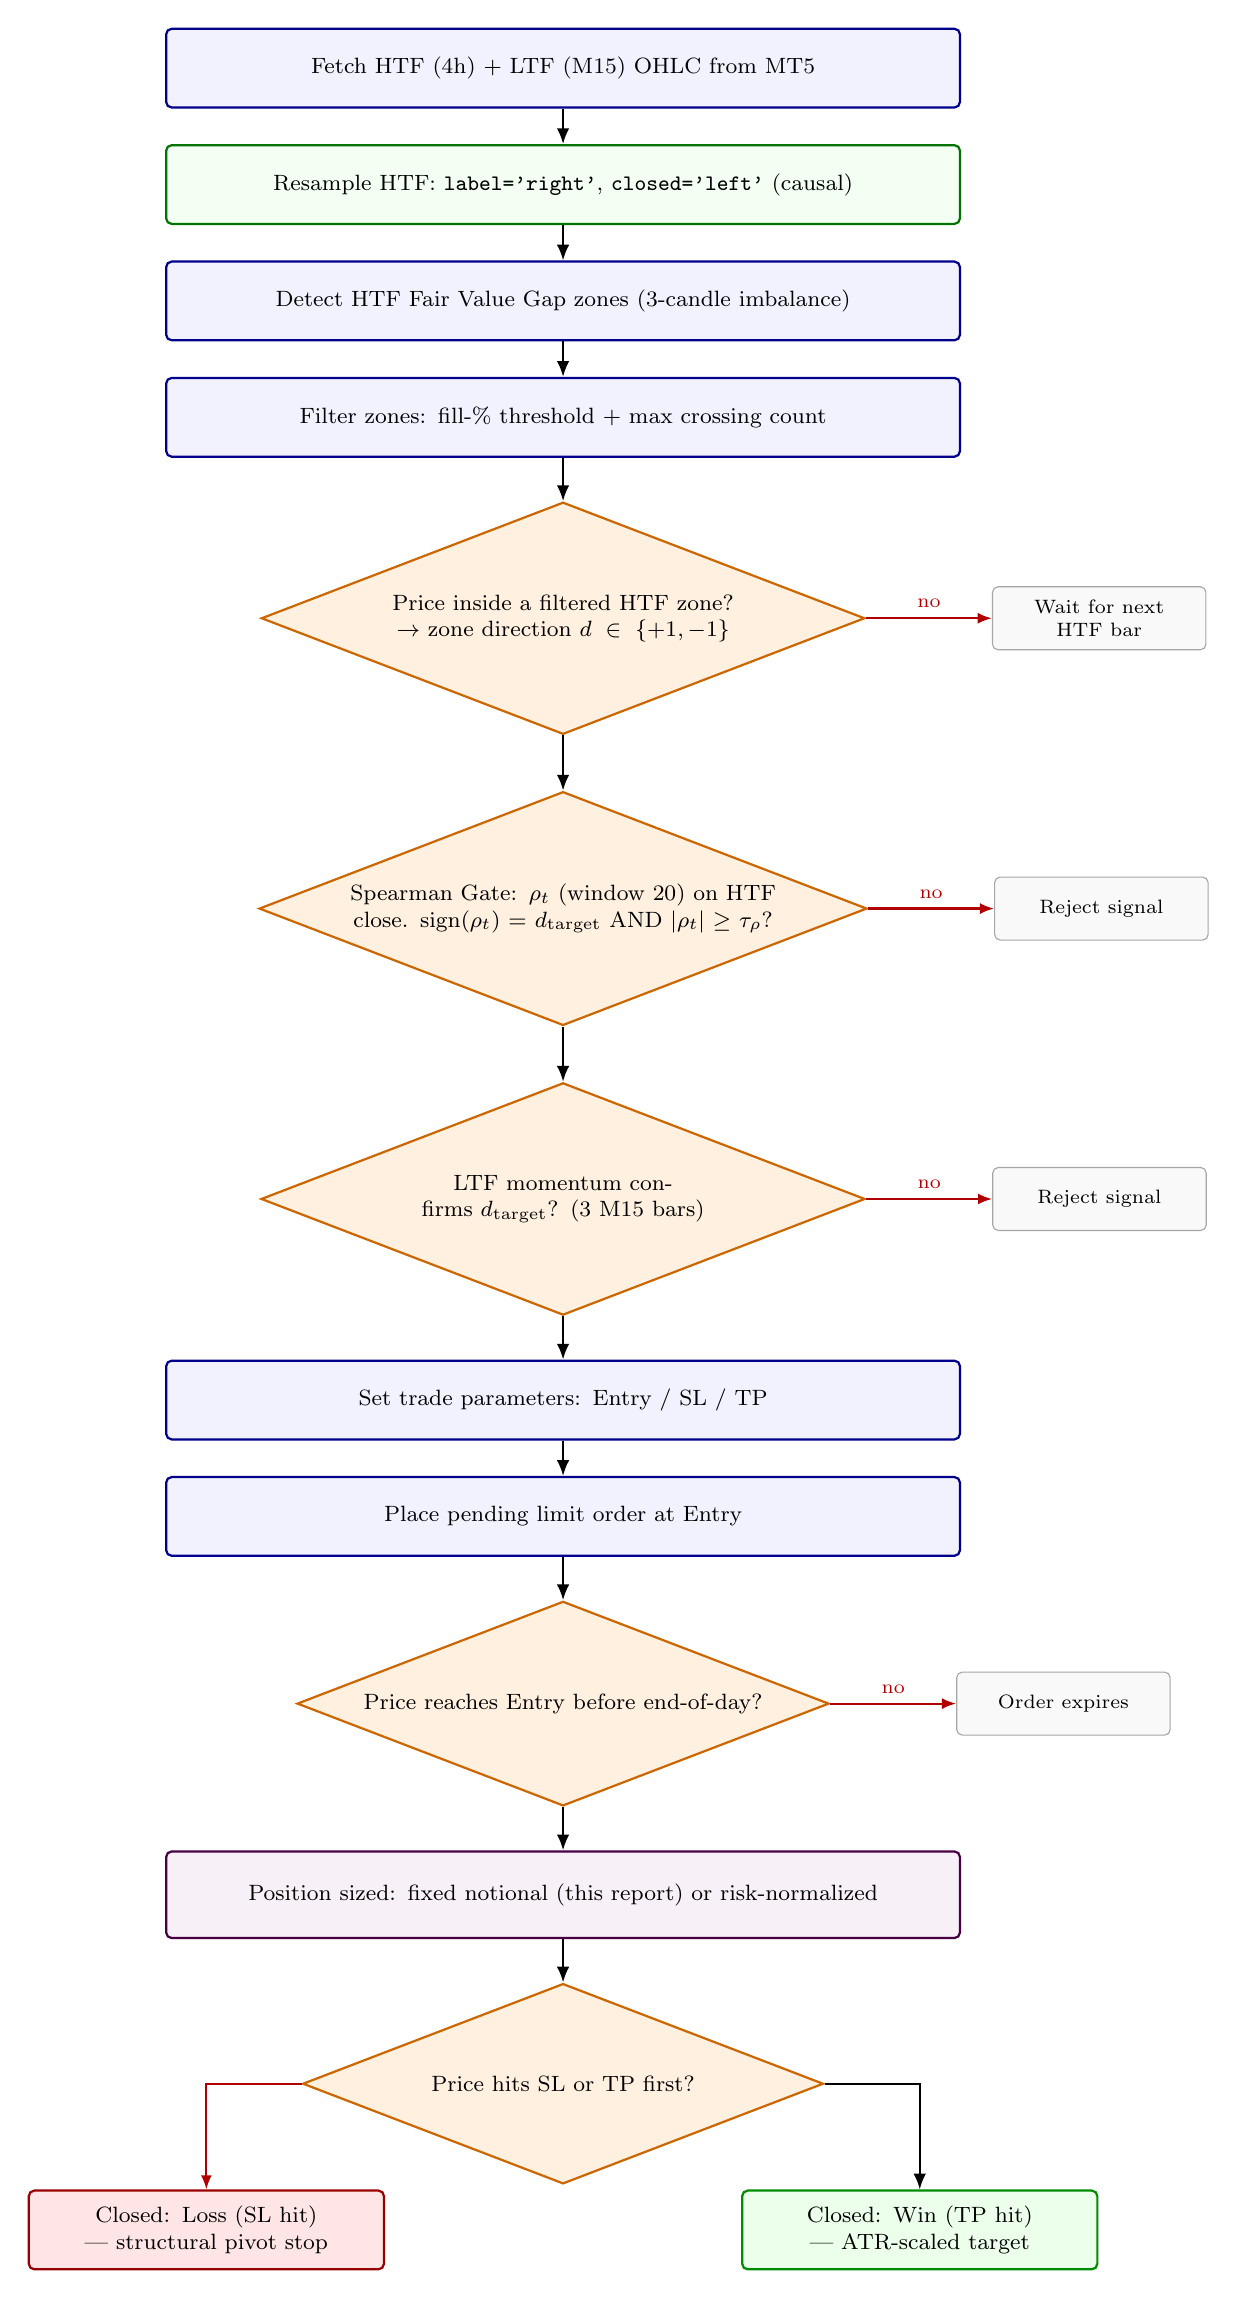
\begin{tikzpicture}[
    font=\footnotesize,
    node distance=0.45cm and 1.6cm,
    proc/.style={rectangle, rounded corners=2pt, draw=blue!55!black, fill=blue!5, thick, text width=9.8cm, align=center, minimum height=1.0cm, inner sep=4pt},
    fix/.style={rectangle, rounded corners=2pt, draw=green!45!black, fill=green!5, thick, text width=9.8cm, align=center, minimum height=1.0cm, inner sep=4pt},
    risk/.style={rectangle, rounded corners=2pt, draw=violet!55!black, fill=violet!6, thick, text width=9.8cm, align=center, minimum height=1.1cm, inner sep=4pt},
    dec/.style={diamond, draw=orange!80!black, fill=orange!12, thick, text width=5.6cm, align=center, inner sep=2pt, aspect=2.6},
    side/.style={rectangle, rounded corners=2pt, draw=gray!70, fill=gray!5, text width=2.5cm, align=center, minimum height=0.8cm, inner sep=3pt, font=\scriptsize},
    term_l/.style={rectangle, rounded corners=2pt, draw=red!60!black, fill=red!10, thick, text width=4.3cm, align=center, minimum height=1.0cm, inner sep=3pt},
    term_w/.style={rectangle, rounded corners=2pt, draw=green!55!black, fill=green!8, thick, text width=4.3cm, align=center, minimum height=1.0cm, inner sep=3pt},
    arr/.style={-{Latex[length=2mm, width=1.6mm]}, thick},
    noarr/.style={-{Latex[length=1.8mm, width=1.4mm]}, thick, red!70!black},
]

\node[proc] (fetch) {Fetch HTF (4h) + LTF (M15) OHLC from MT5};
\node[fix, below=of fetch] (resample) {Resample HTF: \texttt{label='right'}, \texttt{closed='left'} (causal)};
\node[proc, below=of resample] (detect) {Detect HTF Fair Value Gap zones (3-candle imbalance)};
\node[proc, below=of detect] (filter) {Filter zones: fill-\% threshold + max crossing count};
\node[dec, below=0.55cm of filter] (inzone) {Price inside a filtered HTF zone? $\rightarrow$ zone direction $d \in \{+1,-1\}$};
\node[side, right=of inzone] (wait) {Wait for next HTF bar};
\node[dec, below=0.7cm of inzone] (gate) {Spearman Gate: $\rho_t$ (window 20) on HTF close. $\mathrm{sign}(\rho_t) = d_{\text{target}}$ AND $|\rho_t|\ge\tau_\rho$?};
\node[side, right=of gate] (reject1) {Reject signal};
\node[dec, below=0.7cm of gate] (ltf) {LTF momentum confirms $d_{\text{target}}$? (3 M15 bars)};
\node[side, right=of ltf] (reject2) {Reject signal};
\node[proc, below=0.55cm of ltf] (params) {Set trade parameters: Entry / SL / TP};
\node[proc, below=of params] (order) {Place pending limit order at Entry};
\node[dec, below=0.55cm of order] (fill) {Price reaches Entry before end-of-day?};
\node[side, right=of fill] (expire) {Order expires};
\node[risk, below=0.55cm of fill] (size) {Position sized: fixed notional (this report) or risk-normalized};
\node[dec, below=0.55cm of size] (exit) {Price hits SL or TP first?};
\node[term_l, below left=0.7cm and 0.6cm of exit] (loss) {Closed: Loss (SL hit) --- structural pivot stop};
\node[term_w, below right=0.7cm and 0.6cm of exit] (win) {Closed: Win (TP hit) --- ATR-scaled target};

\draw[arr] (fetch) -- (resample);
\draw[arr] (resample) -- (detect);
\draw[arr] (detect) -- (filter);
\draw[arr] (filter) -- (inzone);
\draw[noarr] (inzone) -- node[above,font=\scriptsize]{no} (wait);
\draw[arr] (inzone) -- (gate);
\draw[noarr] (gate) -- node[above,font=\scriptsize]{no} (reject1);
\draw[arr] (gate) -- (ltf);
\draw[noarr] (ltf) -- node[above,font=\scriptsize]{no} (reject2);
\draw[arr] (ltf) -- (params);
\draw[arr] (params) -- (order);
\draw[arr] (order) -- (fill);
\draw[noarr] (fill) -- node[above,font=\scriptsize]{no} (expire);
\draw[arr] (fill) -- (size);
\draw[arr] (size) -- (exit);
\draw[noarr] (exit) -| (loss);
\draw[arr] (exit) -| (win);

\end{tikzpicture}%
}
\caption{MetaFVG signal generation and risk management pipeline, mean-reversion configuration
($d_{\text{target}}=-d$). Orange diamonds are gate/decision points; red edges are rejection paths.}
\label{fig:pipeline}
\end{figure}

\section{Instrument Universe and Fundamental Diversification}
\label{sec:universe}
The backtest universe comprises 14 instruments, selected to be diversified by \emph{fundamental
macro driver} rather than by statistical decorrelation alone:
\begin{itemize}[nosep]
  \item \textbf{7 FX Majors}: AUDUSD, EURUSD, GBPUSD, NZDUSD, USDCAD, USDCHF, USDJPY.
  \item \textbf{4 equity indices, each under a different central bank}: US500 (Federal Reserve),
  GER40 (ECB), JP225 (Bank of Japan), HK50 (Hong Kong Monetary Authority / PBoC linkage).
  \item \textbf{3 additional FX minors}: USDSGD, EURNOK, USDZAR --- chosen as genuinely new
  currency exposures (Singapore, Norway, South Africa) rather than recombinations of the 7 majors.
\end{itemize}
The rationale is explicit: the 7 FX Majors alone share a single dominant common factor (broad USD
strength / risk sentiment) --- their \emph{raw price-return} correlations run $0.3$--$0.9$ in absolute
value once sign convention is accounted for (majors quoting USD as the counter currency move together;
majors quoting it as the base currency move opposite). Adding equity indices under different central
banks and FX minors with no shared currency leg among the existing set is intended to break that single-
factor exposure at the instrument-selection stage, before any portfolio weighting is applied.

\section{Data and Backtest Methodology}
\label{sec:data}
Historical OHLC data is sourced from MetaTrader 5 for all 14 instruments, at M15 (LTF) resolution,
with the HTF (4h) series derived by causal resampling as described in \S\ref{sec:methodology}. The
backtest window spans a 5-year lookback ending July 2026; the blended portfolio's first valid daily
observation is 2022-01-13, once sufficient indicator lookback has accumulated across all 14
instruments. Trades are simulated bar-by-bar: pending limit orders are checked for fill against each
subsequent bar's range, and open positions are checked for SL/TP resolution on every bar thereafter,
with SL evaluated before TP on any bar where both levels are contained in the same bar's range (a
conservative assumption). All results in this report use \textbf{fixed 2\% notional} sizing per trade
(\S\ref{sec:sizing}). Portfolio-level daily returns are computed as the equal-weighted average, across
whichever instruments have a closed trade on a given day, of each instrument's daily P\&L as a fraction
of account equity; days with no closed trades across the entire universe are excluded.

\section{Portfolio Results}
\label{sec:results}
Table~\ref{tab:metrics} reports the standard performance summary for the equal-weight blended
portfolio. Figure~\ref{fig:equity} shows cumulative equity; Figure~\ref{fig:drawdown} shows the
underwater (drawdown) plot.

\begin{table}[H]
\centering
\caption{Equal-weight portfolio performance summary, 5-year backtest, fixed 2\% notional sizing.}
\label{tab:metrics}
\begin{tabular}{lr}
\toprule
Metric & Value \\
\midrule
Total Return & $+0.120\%$ \\
CAGR & $+0.0183\%$ \\
Sharpe (daily, annualized) & $0.518$ \\
Sortino & $0.817$ \\
Calmar & $0.343$ \\
Max Drawdown & $-0.0533\%$ \\
Annualized Volatility & $0.0353\%$ \\
Win Rate (days) & $30.89\%$ \\
Best Day & $+0.0291\%$ \\
Worst Day & $-0.0239\%$ \\
Skew & $1.545$ \\
Tail Ratio & $1.239$ \\
Kelly Criterion & $0.0668$ \\
VaR (95\%) & $-0.0036\%$ \\
CVaR (95\%) & $-0.0072\%$ \\
Recovery Factor & $2.260$ \\
\bottomrule
\end{tabular}
\end{table}

\begin{figure}[H]
\centering
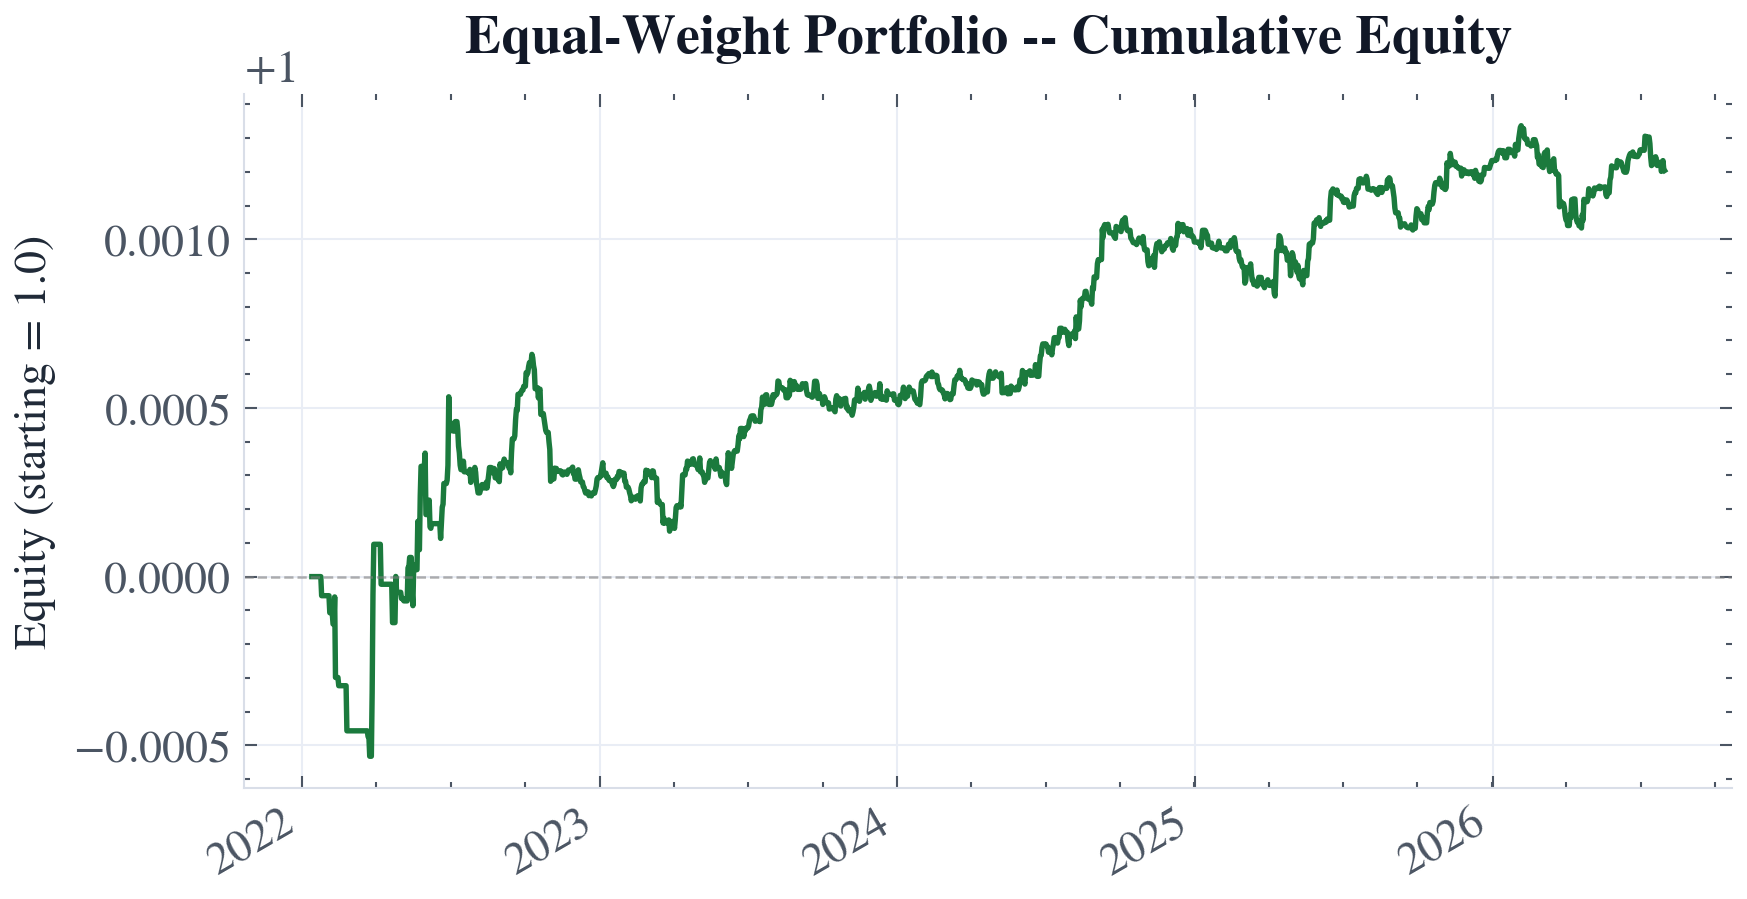
\includegraphics[width=0.92\textwidth]{equal_weight_full/equity_curve.png}
\caption{Equal-weight portfolio cumulative equity (starting value $=1.0$).}
\label{fig:equity}
\end{figure}

\begin{figure}[H]
\centering
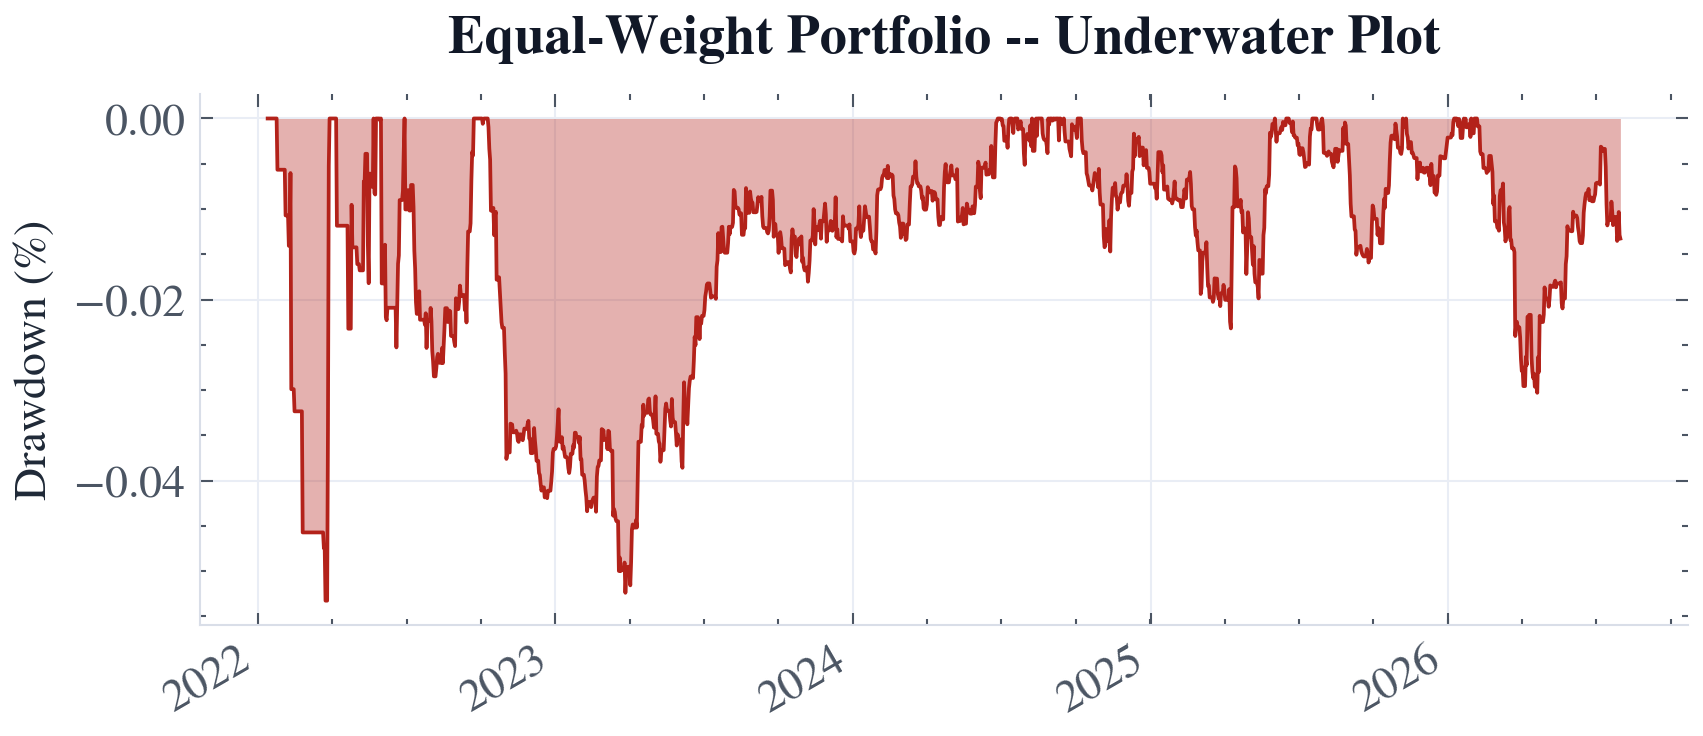
\includegraphics[width=0.92\textwidth]{equal_weight_full/drawdown.png}
\caption{Equal-weight portfolio underwater plot.}
\label{fig:drawdown}
\end{figure}

The return series is markedly positively skewed ($1.545$) with a favorable tail ratio ($1.239$),
consistent with a strategy structured around asymmetric ATR-scaled targets against structural stops
rather than a fixed reward-to-risk ratio. The low day-level win rate ($30.89\%$) alongside a positive
Sharpe indicates the edge is concentrated in the size of winning days, not their frequency ---
expected given the sparse, non-overlapping nature of trade timing across the 14-instrument book (see
\S\ref{sec:correlation}).

\section{Correlation and Diversification Analysis}
\label{sec:correlation}
Figure~\ref{fig:rollcorr} shows the rolling 180-calendar-day average pairwise Pearson correlation
across the 14 instruments' \emph{daily strategy P\&L} (not raw price returns), stepped every 14 days
with a minimum of 15 overlapping observations per pair. Figure~\ref{fig:heatmap} shows the full-sample
static correlation matrix.

\begin{figure}[H]
\centering
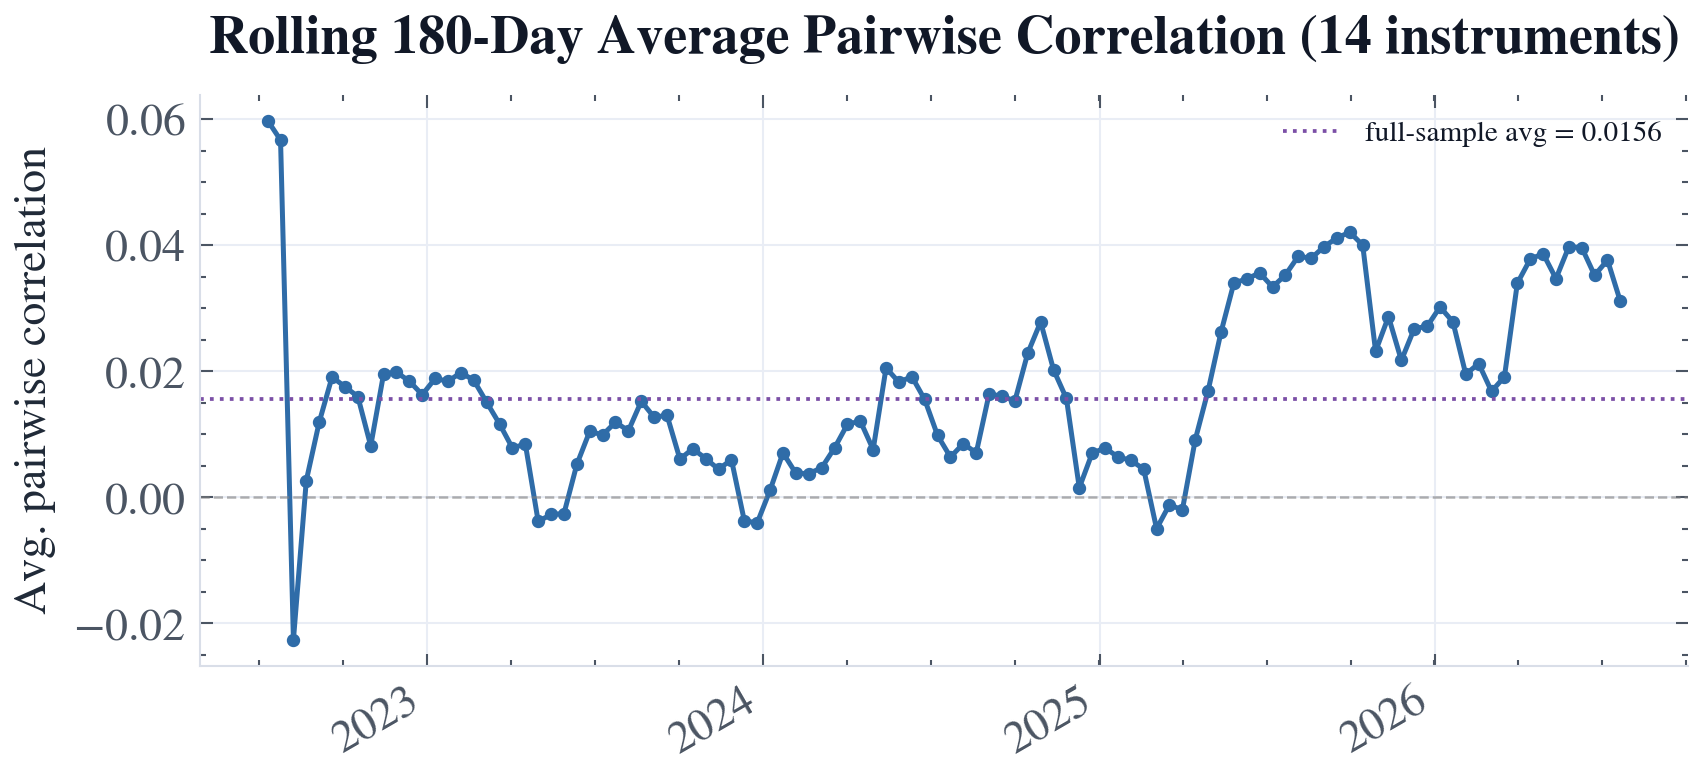
\includegraphics[width=0.92\textwidth]{equal_weight_full/rolling_correlation.png}
\caption{Rolling 180-day average pairwise correlation of traded daily P\&L across the 14-instrument
universe. Dotted line is the full-sample average ($0.0156$).}
\label{fig:rollcorr}
\end{figure}

\begin{figure}[H]
\centering
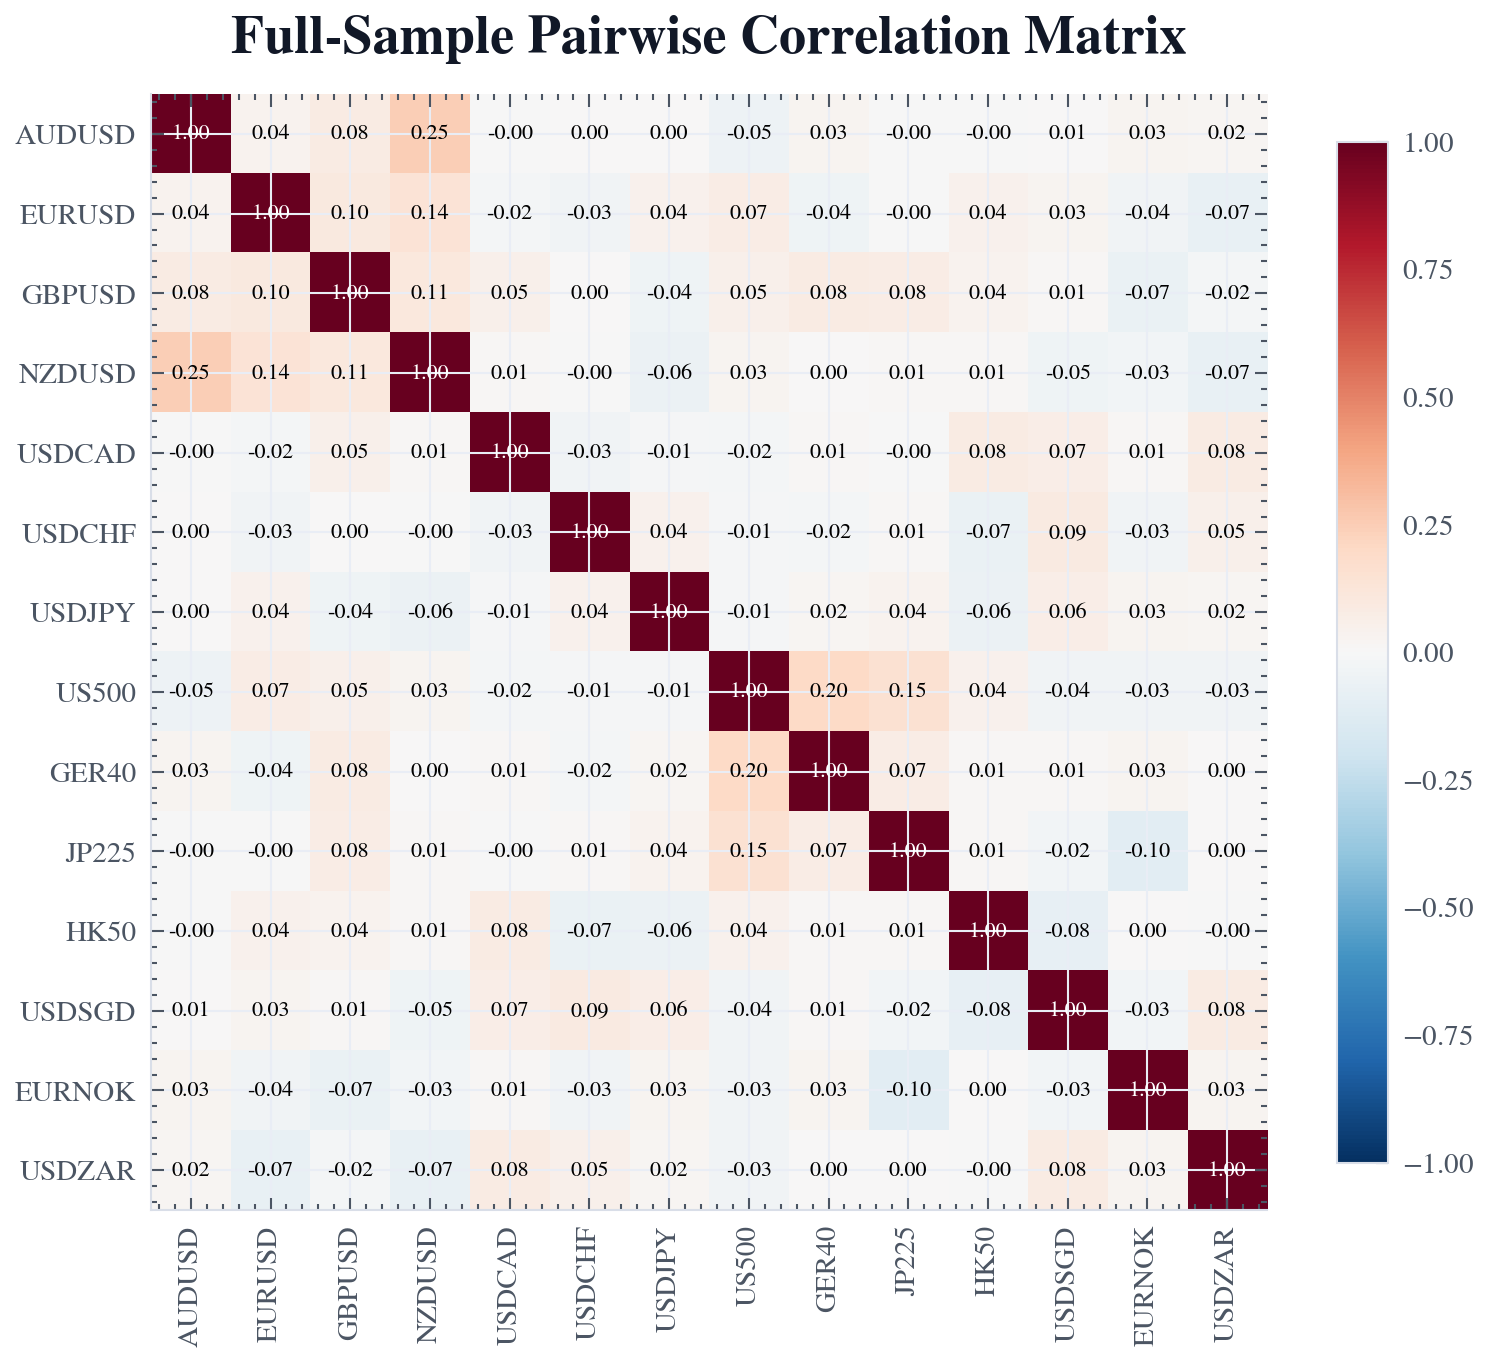
\includegraphics[width=0.78\textwidth]{equal_weight_full/correlation_heatmap.png}
\caption{Full-sample pairwise correlation matrix of the 14 instruments' traded daily P\&L.}
\label{fig:heatmap}
\end{figure}

Two findings are worth separating. First, the \emph{level}: realized correlation between traded P\&L
streams ($0.0156$ average) is roughly an order of magnitude below the underlying instruments' raw
price-return correlation (\S\ref{sec:universe}, $0.3$--$0.9$ in absolute value for the FX Majors
alone). This gap is driven less by the fundamental-driver diversification of \S\ref{sec:universe} than
by the strategy's own sparse, largely non-overlapping trade timing across instruments --- each
instrument only contributes a return on days it has a closed trade, and those days rarely coincide
across the book. Second, the \emph{trend}: rolling correlation is not stationary. It falls to
near-zero (and briefly negative) through 2023--2025 before rising to roughly $0.03$--$0.04$ by
mid-2026 --- still low in absolute terms, but a genuine regime shift worth monitoring rather than a
fixed structural property of the book (\S\ref{sec:limitations}).

\section{Per-Symbol Performance}
\label{sec:persymbol}
Table~\ref{tab:persymbol} reports standalone performance for each instrument's own trade stream.
Equal weighting means every instrument contributes $1/14$ of portfolio capital regardless of its
standalone Sharpe; six of the fourteen have a negative standalone Sharpe.

\begin{table}[H]
\centering
\caption{Per-symbol standalone performance, fixed 2\% notional sizing, sorted by Sharpe.}
\label{tab:persymbol}
\begin{tabular}{lrrrrr}
\toprule
Symbol & Closed Trades & Win Rate & Sharpe & Max DD & Total Return \\
\midrule
NZDUSD & 352 & 28.7\% & \good{$1.141$} & 9.86\% & $+0.333\%$ \\
GBPUSD & 331 & 31.7\% & \good{$1.092$} & 19.42\% & $+0.213\%$ \\
HK50   & 347 & 28.2\% & \good{$0.958$} & 20.31\% & $+0.588\%$ \\
US500  & 399 & 28.6\% & \good{$0.806$} & 15.94\% & $+0.350\%$ \\
AUDUSD & 345 & 24.9\% & \good{$0.799$} & 12.84\% & $+0.250\%$ \\
JP225  & 362 & 29.3\% & \good{$0.541$} & 29.92\% & $+0.369\%$ \\
USDCHF & 339 & 25.7\% & \good{$0.476$} & 11.22\% & $+0.099\%$ \\
USDJPY & 340 & 25.6\% & \bad{$-0.130$} & 16.43\% & $-0.031\%$ \\
EURNOK & 241 & 22.0\% & \bad{$-0.305$} & 17.07\% & $-0.077\%$ \\
GER40  & 384 & 24.2\% & \bad{$-0.476$} & 31.66\% & $-0.195\%$ \\
USDCAD & 347 & 22.8\% & \bad{$-0.477$} & 15.03\% & $-0.084\%$ \\
USDZAR & 359 & 20.6\% & \bad{$-0.609$} & 38.70\% & $-0.221\%$ \\
EURUSD & 374 & 20.9\% & \bad{$-0.634$} & 17.04\% & $-0.111\%$ \\
USDSGD & 319 & 18.5\% & \bad{$-0.691$} & 16.89\% & $-0.102\%$ \\
\bottomrule
\end{tabular}
\end{table}

The negative-Sharpe leg is dominated by USD-quote-as-base pairs (USDJPY, USDCAD, USDZAR, USDSGD) and
GER40; the positive-Sharpe leg spans both FX (NZDUSD, GBPUSD, AUDUSD, USDCHF) and equity indices
(HK50, US500, JP225). This is not obviously attributable to a single macro grouping, which is itself
weak evidence against the mean-reversion edge being a single latent factor trade in disguise.

\section{Parameter Sensitivity Analysis}
\label{sec:sensitivity}
To assess how robust the headline result (\S\ref{sec:results}) is to the exact choice of gate and
risk parameters, the equal-weight 14-instrument portfolio Sharpe was recomputed across a grid of
alternate configurations, holding everything else at the report's baseline values
($w=20$, $\tau_\rho=0.5$, ATR sensitivity $=4.0$).

\subsection{Spearman Gate: Window and Threshold}
Figure~\ref{fig:heatmap-gate} sweeps the rolling window $w\in\{10,15,20,25,30\}$ against the gate
threshold $\tau_\rho\in\{0.3,\ldots,0.7\}$, a $5\times5$ grid of full portfolio backtests. The
baseline cell ($w=20$, $\tau_\rho=0.5$) is outlined.

\begin{figure}[H]
\centering
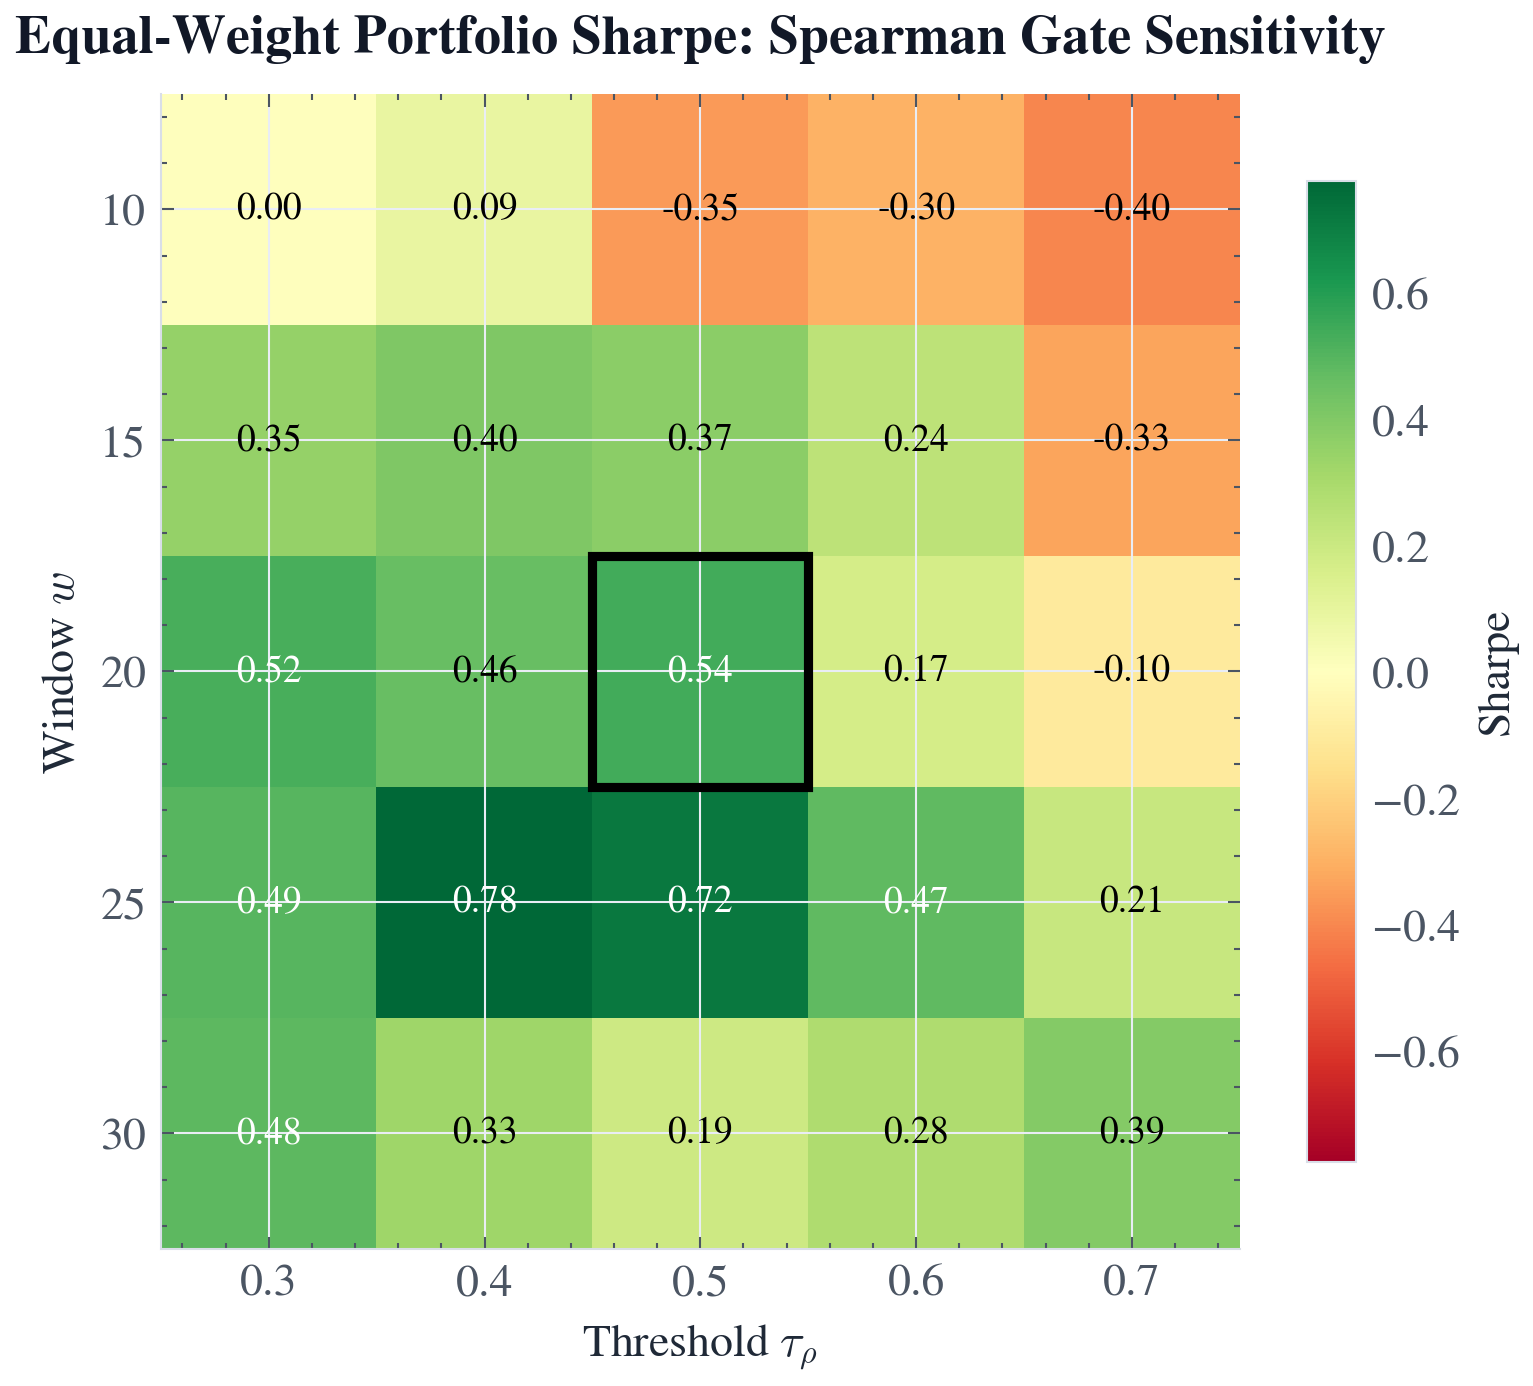
\includegraphics[width=0.75\textwidth]{equal_weight_full/sensitivity_window_threshold_heatmap.png}
\caption{Equal-weight portfolio Sharpe across the Spearman gate's window/threshold grid.}
\label{fig:heatmap-gate}
\end{figure}

The surface is positive across most of the grid ($18$ of $25$ cells $>0$), which is the main
robustness claim: the mean-reversion edge is not a knife-edge artifact of the specific $(20, 0.5)$
choice. That said, two patterns are worth flagging rather than smoothing over. First, short windows
are fragile: $w=10$ is the only row that goes decisively negative, and does so across three of five
thresholds ($\tau_\rho\ge0.5$) --- a 10-bar rank-correlation window is evidently too noisy to gate
reliably at stricter thresholds. Second, and more strikingly, the baseline is \emph{not} the grid
optimum: $w=25,\ \tau_\rho=0.4$ reaches Sharpe $0.777$, well above the baseline's $0.536$
(recomputed on this sweep's slightly different data snapshot; \S\ref{sec:sensitivity-note}), and the
entire $w=25$ row outperforms $w=20$ at every threshold except $0.5$. This was not re-optimized into
a new baseline for this report --- doing so on the same sample that produced the sweep would be
in-sample parameter selection, exactly the failure mode flagged for the current $(20,0.5)$ choice in
\S\ref{sec:limitations}. It is presented here as evidence for a follow-up out-of-sample recalibration,
not as a superior configuration to adopt directly.

\subsection{ATR Sensitivity}
Figure~\ref{fig:atr-line} sweeps ATR sensitivity (the multiplier on ATR$_{14}$ in the TP formula,
\S\ref{sec:params}) from $2.0$ to $6.0$, holding risk\_reward fixed at its default ($2.0$). The two
parameters are not swept independently: TP depends only on their product
($\mathrm{TP}=\text{Entry}\pm\mathrm{ATR}_{14}\times\text{atr\_sensitivity}\times\text{risk\_reward}$,
\texttt{metafvg.py::\_calculate\_trade\_parameters}), so a 2D grid over both would repeat identical
trades along every constant-product diagonal; sweeping one with the other fixed is the non-redundant
version of the same test.

\begin{figure}[H]
\centering
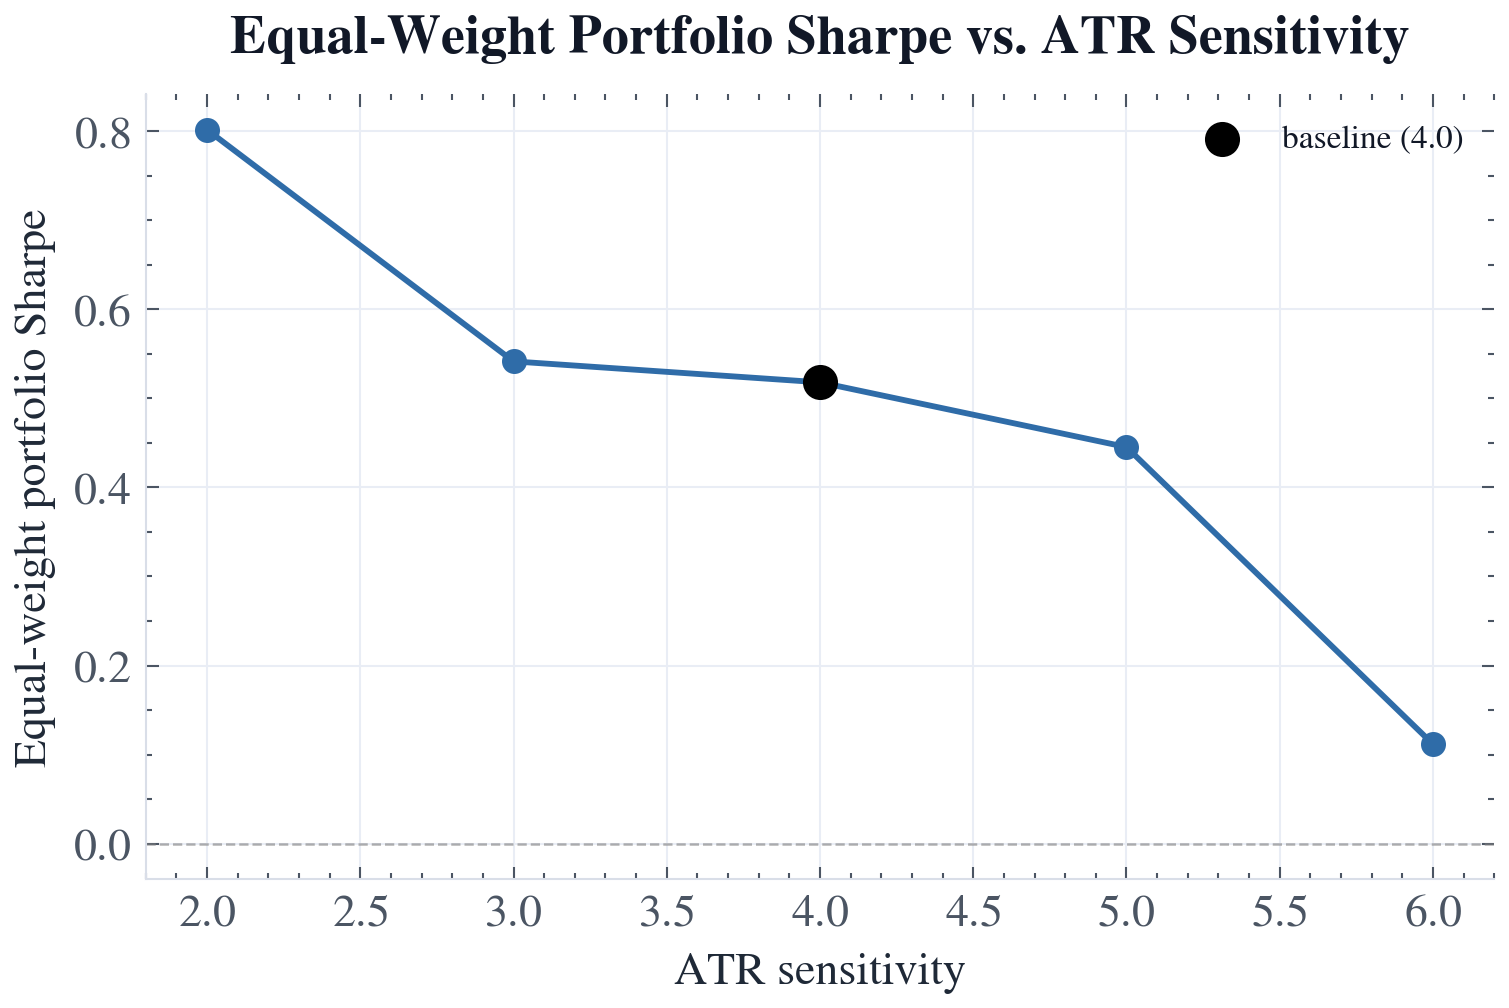
\includegraphics[width=0.75\textwidth]{equal_weight_full/sensitivity_atr_line.png}
\caption{Equal-weight portfolio Sharpe vs.\ ATR sensitivity, risk\_reward fixed at $2.0$.}
\label{fig:atr-line}
\end{figure}

This relationship is monotonic and considerably steeper than the gate parameters: Sharpe falls from
$0.801$ at atr\_sensitivity $=2.0$ to $0.112$ at $=6.0$, roughly a $7\times$ range against the gate
grid's mixed-sign but comparatively narrower spread. Tighter, ATR-scaled targets outperform wider ones
throughout the tested range, with no evidence of an interior optimum above the baseline -- the best
value tested is the smallest one. This is the single largest lever tested in this report and the
strongest candidate for follow-up work: the current default ($4.0$) is not obviously optimal, and the
monotonic trend suggests values below $2.0$ merit testing before concluding where it flattens out.

\subsection{A Note on This Sweep's Data Snapshot}
\label{sec:sensitivity-note}
The OHLC cache underlying this section was fetched on a different day than the cache behind
\S\ref{sec:results}--\ref{sec:persymbol} (a few days' difference in the trailing 5-year window
boundary). Recomputing the exact baseline cell on this sweep's snapshot gives Sharpe $0.536$ against
the $0.518$ reported in Table~\ref{tab:metrics} --- a $3.5\%$ relative difference, consistent with
ordinary sampling noise from the shifted window rather than a discrepancy in methodology.

\section{Exploring Outperforming Parameter Sets}
\label{sec:outperforming}
Both axes of \S\ref{sec:sensitivity} turned up configurations that outperformed the baseline on the
sweep's own Sharpe metric: $w=25,\ \tau_\rho=0.4$ on the gate side, and atr\_sensitivity $=2.0$ on the
risk side. This section takes those two findings further than the sweep did: it backtests each
standout in isolation, and also backtests the two \emph{combined} into a single configuration, to see
whether their effects stack, cancel, or overlap. All four configurations below (baseline plus three
variants) were backtested on the identical OHLC snapshot, so differences are attributable purely to
the parameter changes, not to the snapshot-day noise discussed in \S\ref{sec:sensitivity-note}.

\begin{table}[H]
\centering
\caption{Baseline vs.\ outperforming variants, equal-weight 14-instrument portfolio, identical data
snapshot.}
\label{tab:variants}
\begin{tabular}{lccccccc}
\toprule
Configuration & $w$ & $\tau_\rho$ & ATR sens. & Sharpe & Sortino & Calmar & Max DD \\
\midrule
Baseline & 20 & 0.5 & 4.0 & 0.536 & 0.851 & 0.353 & $-0.0533\%$ \\
Best Gate & 25 & 0.4 & 4.0 & 0.777 & 1.324 & 0.433 & $-0.0796\%$ \\
Best ATR & 20 & 0.5 & 2.0 & 0.801 & 1.407 & 0.563 & $-0.0380\%$ \\
\textbf{Combined Mix} & 25 & 0.4 & 2.0 & \textbf{0.910} & \textbf{1.647} & \textbf{0.787} & $-0.0318\%$ \\
\bottomrule
\end{tabular}
\end{table}

\begin{figure}[H]
\centering
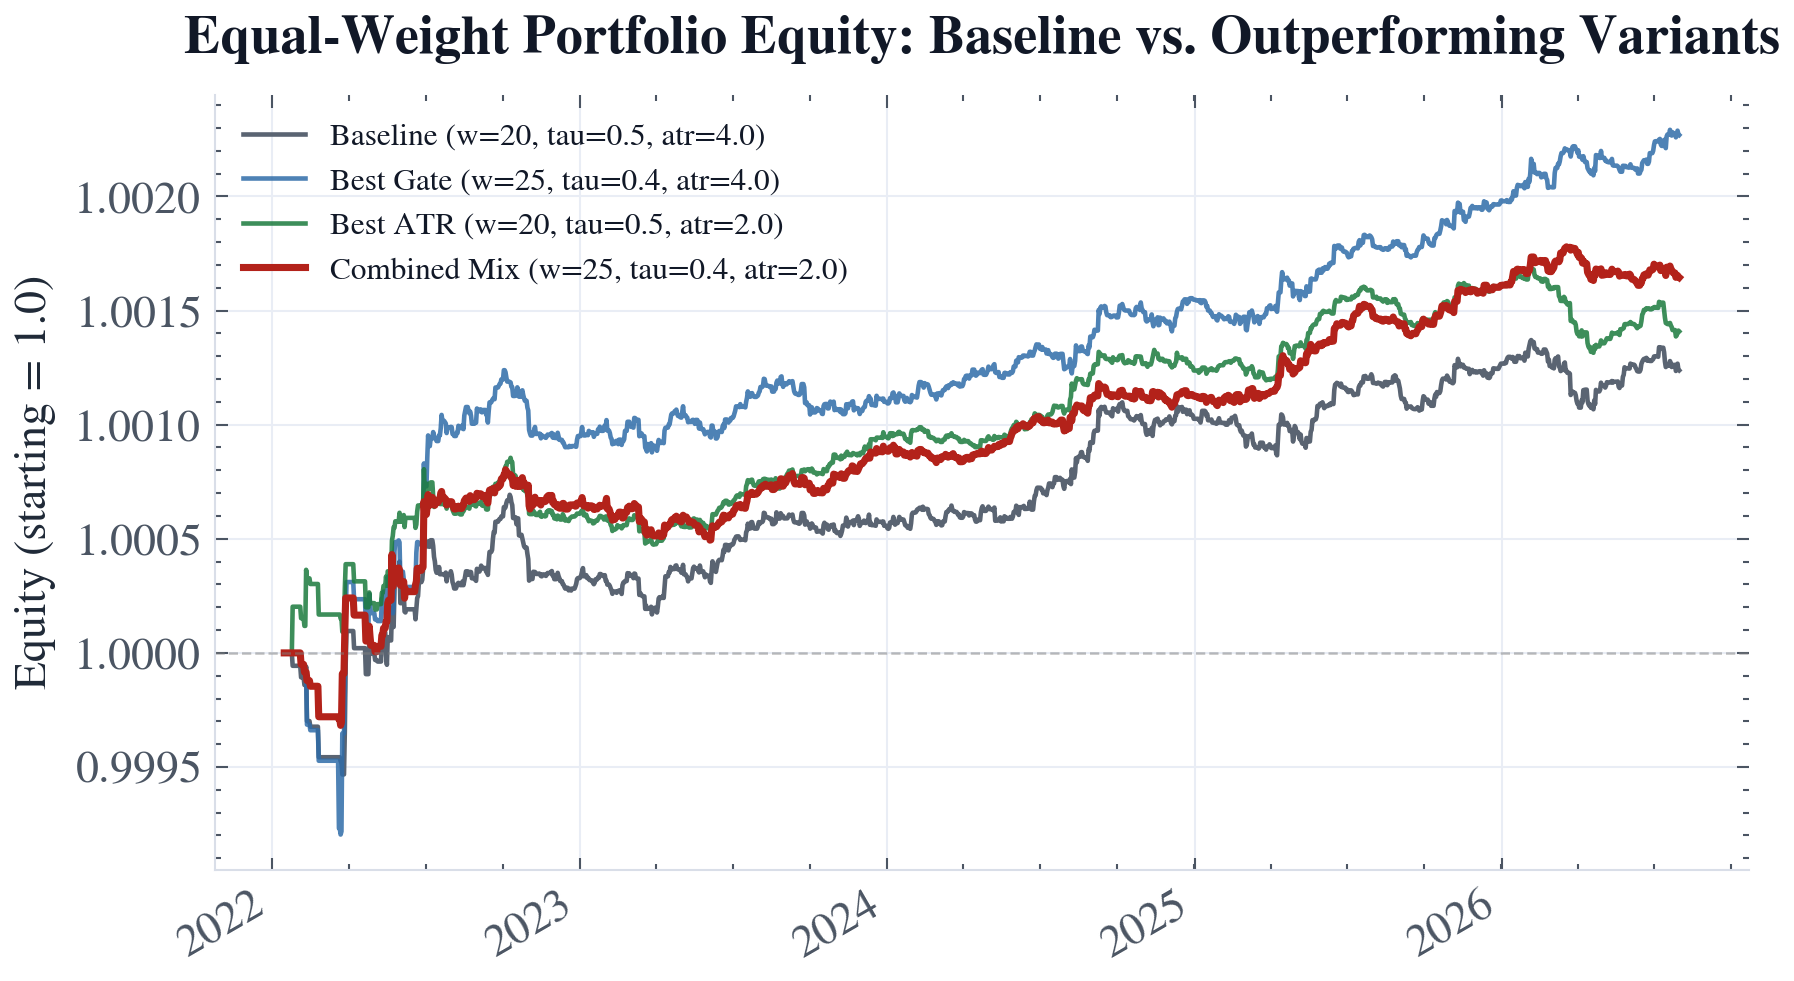
\includegraphics[width=0.92\textwidth]{equal_weight_full/variant_equity_comparison.png}
\caption{Equal-weight portfolio equity: baseline vs.\ the three outperforming variants.}
\label{fig:variant-equity}
\end{figure}

\begin{figure}[H]
\centering
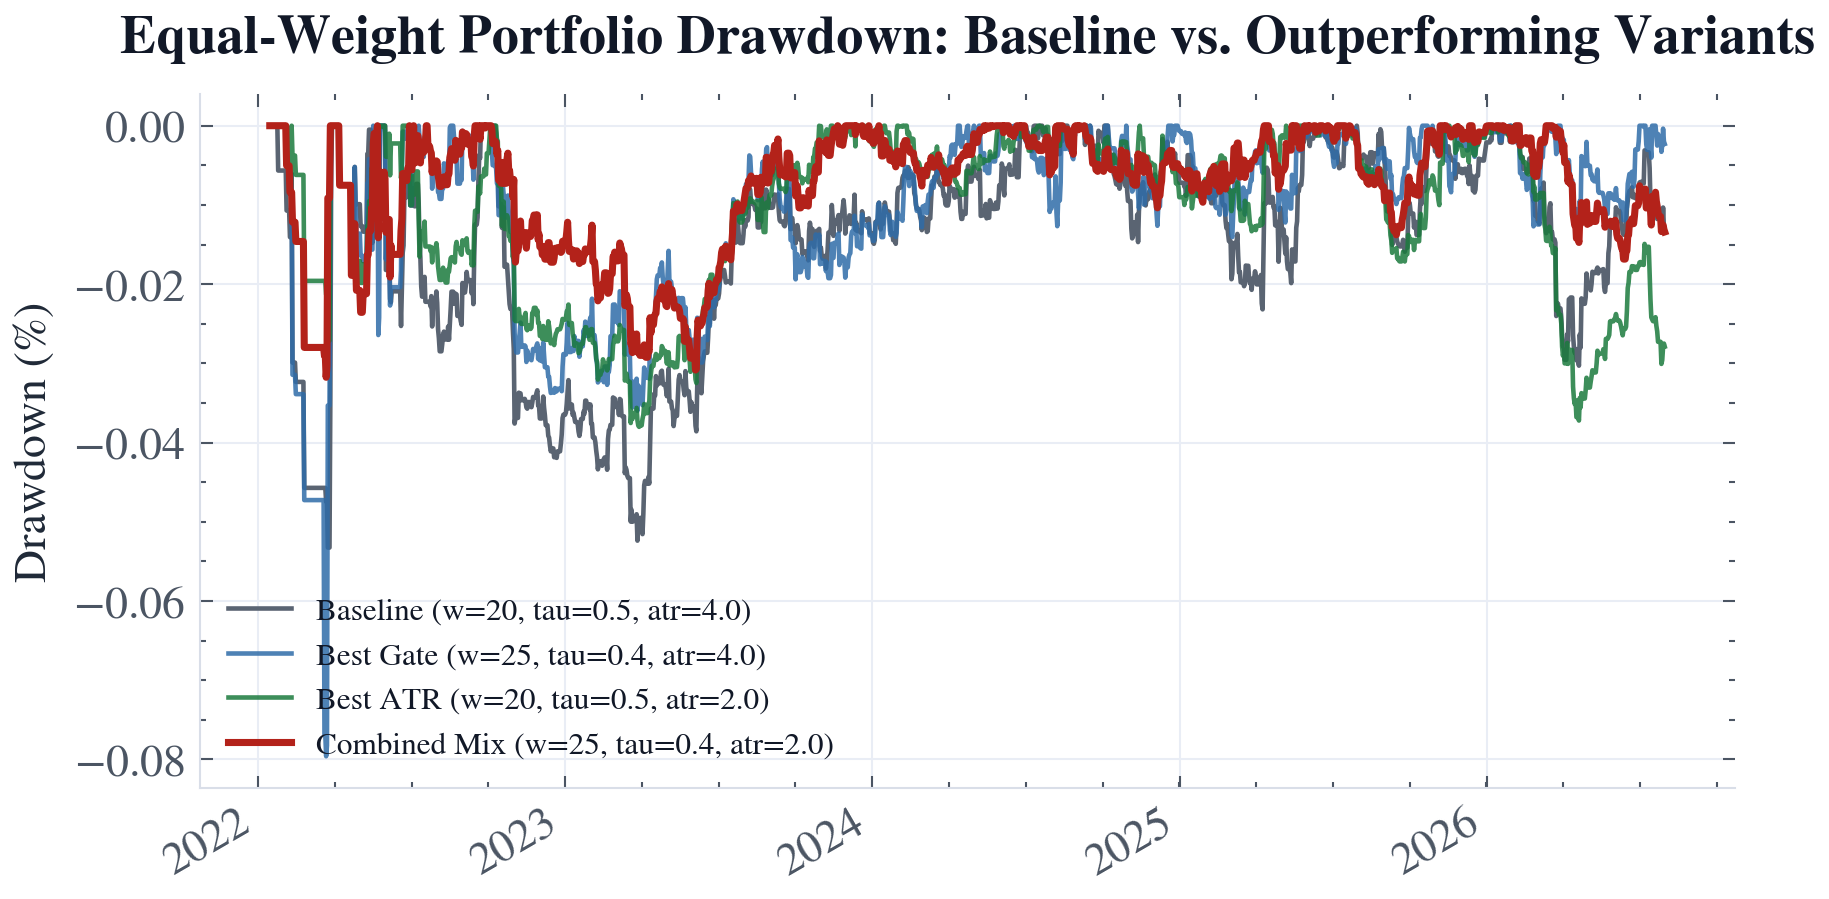
\includegraphics[width=0.92\textwidth]{equal_weight_full/variant_drawdown_comparison.png}
\caption{Equal-weight portfolio drawdown: baseline vs.\ the three outperforming variants.}
\label{fig:variant-drawdown}
\end{figure}

The two levers stack rather than overlap: Combined Mix's Sharpe ($0.910$) exceeds both single-lever
variants (Best Gate $0.777$, Best ATR $0.801$), and its Calmar ($0.787$) is comfortably the best of the
four, with the shallowest max drawdown ($-0.0318\%$). This is evidence the gate parameters and the ATR
sensitivity are addressing genuinely different sources of variance in the strategy, not both proxying
for the same underlying effect.

A less obvious result is visible in Figure~\ref{fig:variant-equity}: \textbf{Best Gate has the highest
raw total return of the four} ($+0.227\%$ vs.\ Combined Mix's $+0.165\%$) but the \emph{lowest}
risk-adjusted ranking among the three variants, because it also carries the highest volatility
($0.0443\%$ annualized vs.\ Combined Mix's $0.0275\%$) and the deepest drawdown of any configuration
tested in this section. Total return and Sharpe do not agree on a winner here --- which one matters
depends on whether the objective is raw return or risk-adjusted return, and this report optimizes for
the latter throughout (matching the convention used for every other comparison in this document, e.g.\
\S\ref{sec:weighting}).

\textbf{This is not a new recommended baseline.} Combined Mix was found by taking the best cell from a
sweep and the best point from a line, both evaluated on the same sample now used to declare a winner
--- exactly the in-sample selection risk already flagged in \S\ref{sec:limitations} for the current
$(20, 0.5, 4.0)$ baseline, now compounded across two dimensions instead of one. The honest reading is
that this section demonstrates the strategy has \emph{more} headroom than the baseline captures, not
that Combined Mix is the configuration to trade live. An out-of-sample or walk-forward validation of
$(25, 0.4, 2.0)$ specifically is the natural next step before treating it as anything more than a
promising candidate.

\section{Alternative Weighting Schemes}
\label{sec:weighting}
A companion study tested whether replacing equal weighting with a correlation-aware allocation could
reduce realized portfolio correlation further without giving up risk-adjusted return. Four schemes
were tested: \textbf{Inverse-Volatility} (naive risk parity, $w_i \propto 1/\sigma_i$), \textbf{Equal
Risk Contribution} (true risk parity via the full covariance matrix), \textbf{Hierarchical Risk
Parity} (correlation-distance clustering with recursive bisection), and \textbf{Inverse
Average-Correlation} ($w_i \propto 1/\bar\rho_i$, the most literal targeting of low correlation).
Table~\ref{tab:weighting} summarizes the outcome; full detail, including per-scheme weight tables and
convergence diagnostics, is in \texttt{weighting\_schemes/comparison\_summary.pdf}.

\begin{table}[H]
\centering
\caption{Weighting scheme comparison, ranked by Sharpe. Wtd.\ Avg.\ Corr.\ and Diversification Ratio
(DR) are computed under each scheme's own weight vector.}
\label{tab:weighting}
\begin{tabular}{lccccc}
\toprule
Scheme & Wtd.\ Avg.\ Corr. & DR & Sharpe & Sortino & Calmar \\
\midrule
\textbf{Equal Weight (baseline)} & 0.0156 & 2.081 & \good{$\mathbf{0.518}$} & 0.817 & 0.343 \\
Inverse Avg-Correlation & \textbf{0.0118} & \textbf{2.110} & \good{$0.483$} & 0.760 & 0.315 \\
Inverse-Volatility & 0.0159 & 1.809 & \good{$0.321$} & 0.504 & 0.200 \\
Equal Risk Contribution & 0.0142 & 1.831 & \good{$0.311$} & 0.488 & 0.191 \\
Hierarchical Risk Parity & 0.0170 & 1.538 & \good{$0.170$} & 0.265 & 0.106 \\
\bottomrule
\end{tabular}
\end{table}

None of the four schemes improved on equal weighting's Sharpe. Three (Inverse-Volatility, ERC, HRP)
allocate on standalone or covariance-implied variance and end up systematically defunding the equity
indices --- precisely the instruments providing the book's real cross-asset diversification, since
they are the ones least correlated with the FX legs --- which worsens both correlation and Sharpe
simultaneously. Only \textbf{Inverse Average-Correlation}, which targets correlation directly rather
than variance, improved both the weighted correlation and the diversification ratio, at a comparatively
small Sharpe cost ($0.518\to0.483$, $-7\%$). The practical conclusion is that this portfolio's low
realized correlation was earned upstream, by fundamental-driver instrument selection
(\S\ref{sec:universe}) and by the strategy's own sparse trade timing (\S\ref{sec:correlation}), not by
weighting --- equal weighting remains the recommended configuration for live use.

\section{Limitations and Future Work}
\label{sec:limitations}
\begin{itemize}[nosep]
  \item \textbf{Not live-traded.} All results are simulated against historical MT5 data; no live
  slippage, requoting, or partial-fill behavior is modeled beyond the conservative SL-before-TP
  same-bar assumption of \S\ref{sec:data}.
  \item \textbf{Single data source.} All OHLC data comes from one MT5 broker feed; results have not
  been cross-validated against an independent data vendor.
  \item \textbf{Gate threshold calibrated in-sample.} $\tau_\rho$ and the rolling window $w=20$ were
  calibrated on the FX Majors subset and carried over to the full 14-instrument universe without a
  separate out-of-sample recalibration step; the sensitivity sweep of \S\ref{sec:sensitivity} finds a
  higher-Sharpe cell elsewhere in the grid ($w=25,\ \tau_\rho=0.4$), which is evidence this concern is
  live rather than theoretical.
  \item \textbf{ATR sensitivity may not be optimally tuned.} \S\ref{sec:sensitivity} finds a
  monotonic Sharpe improvement all the way down to the smallest value tested ($2.0$), with no interior
  optimum found -- the current default ($4.0$) has not been shown to be a good choice, only a
  historically-used one.
  \item \textbf{Sparse per-instrument trade counts.} $241$--$399$ closed trades per instrument over 5
  years ($\sim\!50$--$80$/year) is a modest sample for per-symbol Sharpe estimates in
  Table~\ref{tab:persymbol}; the portfolio-level result in Table~\ref{tab:metrics} is more robust by
  pooling across instruments.
  \item \textbf{Non-stationary correlation.} The rolling correlation trend of \S\ref{sec:correlation}
  rising toward $0.03$--$0.04$ into 2026 warrants monitoring --- a continued rise would erode the
  diversification benefit the equal-weight conclusion of \S\ref{sec:weighting} currently rests on.
  \item \textbf{Risk-normalized sizing underperforms fixed notional here} (\S\ref{sec:sizing}), which
  is counterintuitive relative to typical portfolio theory and not fully explained; worth further
  investigation before ruling it out for other configurations.
\end{itemize}

\section{Conclusion}
The Spearman mean-reversion configuration of MetaFVG, blended equally across a 14-instrument,
fundamentally-diversified universe, produces a Sharpe of $0.518$ with realized cross-instrument
correlation an order of magnitude below the underlying instruments' structural correlation. That
diversification benefit is attributable primarily to instrument selection and the strategy's own
sparse trade timing rather than to portfolio weighting: four correlation-aware weighting schemes were
tested and none improved on simple equal weighting. The strongest caveats are a rising rolling-
correlation trend into 2026 and the fact that gate thresholds were calibrated on a subset of the full
universe --- both flagged as priorities for follow-up work rather than settled findings.

\appendix
\section{Full Trade List}
\label{sec:appendix-trades}
Every closed trade from the baseline configuration ($w=20$, $\tau_\rho=0.5$, ATR sensitivity $=4.0$,
fixed 2\% notional sizing, \S\ref{sec:results}), listed chronologically by entry time across all 14
instruments. Entry, SL, TP, and Exit are raw price levels in each instrument's native quote units
(not normalized across instruments); PnL is the raw price-difference return per unit
($(\text{exit}-\text{entry})\times\text{direction}$, matching the definition in
\texttt{metafvg\_backtest.py::Trade.pnl}), not a dollar or percent-of-equity figure. \textbf{No lot
size / position size column is included}: this backtest engine has no concept of real MT5 lot or
contract sizing at the individual-trade level anywhere in the codebase --- portfolio-level statistics
throughout this report (Table~\ref{tab:metrics} onward) are computed from vectorbt's abstract
\texttt{size\_type=`percent'} sizing (a fixed 2\% of current equity per trade, chosen for
cross-instrument comparability of percentage-based statistics, not as a claim about real position
sizing), and live trading (\texttt{metafvg.py}) uses a static, externally-configured lot size rather
than a per-trade computed one. Direction (long/short) is recoverable from the price levels: SL $<$
Entry $<$ TP indicates a long trade, SL $>$ Entry $>$ TP a short.

\begin{longtable}{@{}l r r r r r@{}}
\caption{Full baseline trade list (window $w=20$, $\tau_\rho=0.5$, ATR sensitivity $=4.0$, fixed 2\% notional sizing) --- all 4,837 closed trades across the 14-instrument universe, chronological by entry time.} \label{tab:trades} \\
\toprule
Asset & Entry & SL & TP & Exit & PnL \\
\midrule
\endfirsthead
\multicolumn{6}{l}{\small\itshape (Table~\ref{tab:trades} continued)} \\
\toprule
Asset & Entry & SL & TP & Exit & PnL \\
\midrule
\endhead
\midrule
\multicolumn{6}{r}{\small\itshape continued on next page} \\
\endfoot
\bottomrule
\endlastfoot
HK50 & 24383 & 24452 & 23890 & 24452 & \bad{$-69$} \\
HK50 & 24469 & 24530 & 24236 & 24530 & \bad{$-61.75$} \\
HK50 & 24435 & 24476 & 24134 & 24476 & \bad{$-41$} \\
HK50 & 24971 & 24646 & 25320 & 24646 & \bad{$-325$} \\
HK50 & 24765 & 24646 & 25032 & 25032 & \good{$+267.29$} \\
HK50 & 24908 & 24769 & 25110 & 24769 & \bad{$-139.25$} \\
HK50 & 24530 & 24560 & 24363 & 24560 & \bad{$-30$} \\
HK50 & 22908 & 23062 & 22403 & 23062 & \bad{$-153.25$} \\
HK50 & 22072 & 22092 & 21876 & 22092 & \bad{$-19.15$} \\
HK50 & 21536 & 21598 & 21128 & 21598 & \bad{$-62.5$} \\
HK50 & 21645 & 21192 & 22363 & 22363 & \good{$+718.43$} \\
HK50 & 22002 & 22041 & 21693 & 22041 & \bad{$-39.5$} \\
HK50 & 21818 & 21900 & 21651 & 21900 & \bad{$-82$} \\
HK50 & 20492 & 20681 & 20175 & 20681 & \bad{$-189$} \\
HK50 & 20518 & 20563 & 20310 & 20563 & \bad{$-45$} \\
GER40 & 14139 & 14148 & 14055 & 14148 & \bad{$-9$} \\
GER40 & 14078 & 14168 & 13877 & 13877 & \good{$+201.63$} \\
GER40 & 13789 & 13854 & 13474 & 13854 & \bad{$-64.8$} \\
GER40 & 13969 & 14008 & 13782 & 14008 & \bad{$-38.8$} \\
HK50 & 20262 & 20290 & 20072 & 20290 & \bad{$-28$} \\
HK50 & 19872 & 19917 & 19482 & 19482 & \good{$+390.43$} \\
GER40 & 13988 & 13894 & 14181 & 13894 & \bad{$-94.2$} \\
GER40 & 14000 & 13894 & 14217 & 13894 & \bad{$-106$} \\
JP225 & 26719 & 26859 & 26447 & 26859 & \bad{$-140$} \\
HK50 & 20612 & 20771 & 20262 & 20262 & \good{$+349.43$} \\
US500 & 4084.5 & 4098.5 & 4060.7 & 4060.7 & \good{$+23.857$} \\
US500 & 4079.8 & 4086.8 & 4049 & 4086.8 & \bad{$-7$} \\
GER40 & 14006 & 14151 & 13756 & 14151 & \bad{$-144.8$} \\
US500 & 3929.4 & 3810.2 & 4018.8 & 4018.8 & \good{$+89.469$} \\
GER40 & 14108 & 14088 & 14236 & 14088 & \bad{$-20$} \\
US500 & 3920.6 & 3810.2 & 4021.6 & 4021.6 & \good{$+100.99$} \\
GER40 & 14043 & 13845 & 14290 & 14290 & \good{$+247.22$} \\
JP225 & 26829 & 26869 & 26598 & 26598 & \good{$+231.43$} \\
JP225 & 26664 & 26809 & 26339 & 26809 & \bad{$-145$} \\
JP225 & 26723 & 26813 & 26382 & 26813 & \bad{$-90$} \\
JP225 & 26778 & 26813 & 26434 & 26813 & \bad{$-35$} \\
GER40 & 14038 & 14097 & 13876 & 14097 & \bad{$-59.4$} \\
JP225 & 26654 & 26682 & 26436 & 26682 & \bad{$-27.5$} \\
JP225 & 26769 & 26903 & 26290 & 26903 & \bad{$-133.5$} \\
US500 & 4046.6 & 3987.5 & 4118 & 4118 & \good{$+71.417$} \\
US500 & 4055.8 & 4049.7 & 4106.2 & 4049.7 & \bad{$-6.15$} \\
US500 & 4136.3 & 4145.8 & 4054.1 & 4145.8 & \bad{$-9.5$} \\
GER40 & 14443 & 14499 & 14275 & 14499 & \bad{$-56$} \\
GER40 & 14474 & 14488 & 14362 & 14488 & \bad{$-14$} \\
GER40 & 14434 & 14449 & 14274 & 14449 & \bad{$-15$} \\
US500 & 4123.5 & 4167.3 & 4049.6 & 4167.3 & \bad{$-43.75$} \\
GER40 & 14343 & 14354 & 14261 & 14354 & \bad{$-11$} \\
US500 & 4092.1 & 4130 & 4055.2 & 4130 & \bad{$-37.92$} \\
GER40 & 14552 & 14482 & 14632 & 14632 & \good{$+80$} \\
HK50 & 21698 & 21893 & 21266 & 21893 & \bad{$-195.5$} \\
HK50 & 21626 & 21648 & 21501 & 21501 & \good{$+125.23$} \\
HK50 & 21552 & 21648 & 21243 & 21648 & \bad{$-96$} \\
JP225 & 27984 & 28064 & 27696 & 28064 & \bad{$-80$} \\
HK50 & 21661 & 21757 & 21088 & 21757 & \bad{$-96$} \\
US500 & 4127.5 & 4139.5 & 4048 & 4139.5 & \bad{$-12$} \\
GER40 & 14586 & 14607 & 14492 & 14607 & \bad{$-21$} \\
US500 & 4151.9 & 4158.9 & 4122.7 & 4158.9 & \bad{$-7$} \\
GER40 & 14495 & 14618 & 14340 & 14340 & \good{$+155.43$} \\
US500 & 4156.1 & 4158.9 & 4126.6 & 4158.9 & \bad{$-2.75$} \\
JP225 & 26085 & 25946 & 26447 & 25946 & \bad{$-138.5$} \\
HK50 & 21031 & 20885 & 21371 & 20885 & \bad{$-146$} \\
HK50 & 21181 & 21003 & 21454 & 21454 & \good{$+272.29$} \\
US500 & 3762.7 & 3782.9 & 3730.7 & 3730.7 & \good{$+32$} \\
GER40 & 13224 & 13265 & 13138 & 13138 & \good{$+86.051$} \\
US500 & 3760.7 & 3782.9 & 3730.9 & 3782.9 & \bad{$-22.15$} \\
US500 & 3760.3 & 3746.5 & 3798.6 & 3746.5 & \bad{$-13.75$} \\
US500 & 3762.8 & 3734.3 & 3829.5 & 3829.5 & \good{$+66.714$} \\
GER40 & 13163 & 13198 & 13014 & 13198 & \bad{$-35.9$} \\
HK50 & 22310 & 22595 & 21962 & 21962 & \good{$+348.57$} \\
JP225 & 26816 & 27276 & 26584 & 26584 & \good{$+232.29$} \\
JP225 & 26762 & 26847 & 26470 & 26847 & \bad{$-85$} \\
GER40 & 13125 & 13136 & 13011 & 13136 & \bad{$-11$} \\
HK50 & 21998 & 22099 & 21648 & 22099 & \bad{$-101$} \\
JP225 & 26743 & 26866 & 26315 & 26315 & \good{$+428.57$} \\
GER40 & 12972 & 13039 & 12882 & 12882 & \good{$+90.474$} \\
HK50 & 22039 & 22060 & 21917 & 21917 & \good{$+122.86$} \\
US500 & 3814.6 & 3819.1 & 3785.9 & 3785.9 & \good{$+28.72$} \\
GER40 & 12974 & 12996 & 12861 & 12861 & \good{$+112.55$} \\
JP225 & 26298 & 26348 & 25938 & 26348 & \bad{$-50$} \\
HK50 & 21776 & 22088 & 21559 & 21559 & \good{$+217.57$} \\
US500 & 3812.4 & 3815.9 & 3781.8 & 3815.9 & \bad{$-3.5$} \\
JP225 & 26423 & 26493 & 25993 & 26493 & \bad{$-70$} \\
JP225 & 26386 & 26428 & 26064 & 26428 & \bad{$-42.5$} \\
US500 & 3761.4 & 3793.4 & 3709.5 & 3793.4 & \bad{$-32$} \\
US500 & 3773.3 & 3793.4 & 3722.1 & 3793.4 & \bad{$-20.07$} \\
GER40 & 12854 & 12806 & 13020 & 12806 & \bad{$-48.5$} \\
GER40 & 12887 & 12841 & 13003 & 12841 & \bad{$-45.72$} \\
GER40 & 12829 & 12783 & 13052 & 12783 & \bad{$-46.2$} \\
US500 & 3829.6 & 3846.9 & 3768 & 3846.9 & \bad{$-17.25$} \\
JP225 & 26638 & 26533 & 27004 & 27004 & \good{$+365.71$} \\
GER40 & 12983 & 12756 & 13328 & 12756 & \bad{$-227.5$} \\
HK50 & 21699 & 21668 & 21820 & 21668 & \bad{$-31$} \\
JP225 & 26580 & 26632 & 26449 & 26632 & \bad{$-52.5$} \\
GER40 & 12727 & 12767 & 12539 & 12767 & \bad{$-40.6$} \\
JP225 & 26471 & 26696 & 26115 & 26696 & \bad{$-225$} \\
GER40 & 12794 & 12823 & 12594 & 12823 & \bad{$-29.2$} \\
US500 & 3797.7 & 3804 & 3771.5 & 3804 & \bad{$-6.25$} \\
US500 & 3884.1 & 3876.6 & 3903.5 & 3903.5 & \good{$+19.389$} \\
US500 & 3842.2 & 3845.2 & 3822.3 & 3845.2 & \bad{$-3$} \\
HK50 & 20685 & 20768 & 20335 & 20768 & \bad{$-83$} \\
US500 & 3846.4 & 3852.2 & 3807.7 & 3852.2 & \bad{$-5.75$} \\
JP225 & 27783 & 27643 & 28085 & 27643 & \bad{$-140$} \\
GER40 & 13182 & 13200 & 13116 & 13116 & \good{$+66.286$} \\
HK50 & 20856 & 20905 & 20523 & 20905 & \bad{$-48.75$} \\
GER40 & 13143 & 13198 & 12961 & 13198 & \bad{$-54.5$} \\
HK50 & 20848 & 20966 & 20631 & 20631 & \good{$+216.94$} \\
JP225 & 27469 & 27644 & 27229 & 27644 & \bad{$-175$} \\
GER40 & 13104 & 13140 & 12853 & 13140 & \bad{$-36$} \\
US500 & 3925.1 & 3936.6 & 3876.5 & 3936.6 & \bad{$-11.5$} \\
JP225 & 27474 & 27519 & 27272 & 27519 & \bad{$-45$} \\
HK50 & 20719 & 20746 & 20515 & 20746 & \bad{$-27$} \\
GER40 & 13149 & 13207 & 13030 & 13207 & \bad{$-58$} \\
GER40 & 13161 & 13195 & 12979 & 13195 & \bad{$-34$} \\
GER40 & 13179 & 13205 & 12996 & 13205 & \bad{$-26$} \\
GER40 & 13208 & 13255 & 13104 & 13104 & \good{$+104.2$} \\
GER40 & 13218 & 13255 & 13095 & 13095 & \good{$+122.49$} \\
JP225 & 27837 & 27607 & 28070 & 28070 & \good{$+232.86$} \\
EURUSD & 1.0189 & 1.0219 & 1.0075 & 1.0219 & \bad{$-0.00305$} \\
EURUSD & 1.0192 & 1.0145 & 1.0302 & 1.0145 & \bad{$-0.00467$} \\
AUDUSD & 0.69895 & 0.69681 & 0.70289 & 0.69681 & \bad{$-0.00214$} \\
AUDUSD & 0.69851 & 0.69681 & 0.70244 & 0.69681 & \bad{$-0.0017$} \\
USDZAR & 16.578 & 16.542 & 16.65 & 16.65 & \good{$+0.0722$} \\
USDZAR & 16.615 & 16.542 & 16.701 & 16.542 & \bad{$-0.07304$} \\
NZDUSD & 0.62904 & 0.62763 & 0.63419 & 0.63419 & \good{$+0.0051543$} \\
USDZAR & 16.63 & 16.618 & 16.722 & 16.618 & \bad{$-0.0121$} \\
JP225 & 27616 & 27920 & 27250 & 27920 & \bad{$-303.5$} \\
GER40 & 13425 & 13435 & 13327 & 13327 & \good{$+98$} \\
GBPUSD & 1.2218 & 1.2263 & 1.2143 & 1.2143 & \good{$+0.0075029$} \\
USDCAD & 1.2859 & 1.2875 & 1.2808 & 1.2875 & \bad{$-0.0016$} \\
USDCAD & 1.287 & 1.2875 & 1.2815 & 1.2875 & \bad{$-0.00049$} \\
USDSGD & 1.3802 & 1.3813 & 1.3735 & 1.3813 & \bad{$-0.00107$} \\
EURUSD & 1.0168 & 1.0172 & 1.0141 & 1.0172 & \bad{$-0.00044$} \\
GER40 & 13431 & 13446 & 13331 & 13446 & \bad{$-15$} \\
USDZAR & 16.777 & 16.846 & 16.646 & 16.846 & \bad{$-0.06951$} \\
HK50 & 19809 & 19937 & 19413 & 19937 & \bad{$-128.25$} \\
NZDUSD & 0.62524 & 0.62576 & 0.62041 & 0.62576 & \bad{$-0.00052$} \\
USDJPY & 132.93 & 133.9 & 131.27 & 133.9 & \bad{$-0.97$} \\
USDSGD & 1.3814 & 1.3845 & 1.3771 & 1.3771 & \good{$+0.00428$} \\
GER40 & 13473 & 13488 & 13336 & 13488 & \bad{$-15$} \\
EURUSD & 1.0186 & 1.02 & 1.0119 & 1.02 & \bad{$-0.00141$} \\
NZDUSD & 0.62472 & 0.62723 & 0.61778 & 0.62723 & \bad{$-0.00251$} \\
EURUSD & 1.0161 & 1.017 & 1.0131 & 1.017 & \bad{$-0.00095$} \\
EURUSD & 1.0163 & 1.0176 & 1.013 & 1.0176 & \bad{$-0.00125$} \\
USDZAR & 16.775 & 16.735 & 16.901 & 16.735 & \bad{$-0.0406$} \\
USDJPY & 133.93 & 133.66 & 134.68 & 133.66 & \bad{$-0.266$} \\
USDZAR & 16.583 & 16.579 & 16.645 & 16.579 & \bad{$-0.00413$} \\
HK50 & 20254 & 20191 & 20375 & 20191 & \bad{$-63$} \\
HK50 & 20251 & 20191 & 20346 & 20191 & \bad{$-60$} \\
GER40 & 13672 & 13666 & 13717 & 13666 & \bad{$-6.25$} \\
GER40 & 13659 & 13645 & 13724 & 13645 & \bad{$-14$} \\
HK50 & 20196 & 20116 & 20471 & 20116 & \bad{$-80$} \\
USDZAR & 16.59 & 16.569 & 16.641 & 16.569 & \bad{$-0.02071$} \\
HK50 & 20043 & 20002 & 20314 & 20002 & \bad{$-41$} \\
EURUSD & 1.0176 & 1.0173 & 1.021 & 1.0173 & \bad{$-0.00033$} \\
EURUSD & 1.018 & 1.0159 & 1.0213 & 1.0213 & \good{$+0.0033486$} \\
NZDUSD & 0.62526 & 0.62295 & 0.62851 & 0.62851 & \good{$+0.0032514$} \\
USDZAR & 16.789 & 16.767 & 16.847 & 16.767 & \bad{$-0.02248$} \\
EURUSD & 1.0173 & 1.0159 & 1.0204 & 1.0204 & \good{$+0.0031429$} \\
EURNOK & 9.926 & 9.9355 & 9.8697 & 9.9355 & \bad{$-0.00951$} \\
EURNOK & 9.9266 & 9.9281 & 9.8803 & 9.9281 & \bad{$-0.00145$} \\
AUDUSD & 0.69825 & 0.69925 & 0.69527 & 0.69925 & \bad{$-0.001$} \\
NZDUSD & 0.62832 & 0.62928 & 0.6259 & 0.62928 & \bad{$-0.00096$} \\
US500 & 4151.3 & 4155.3 & 4129.1 & 4129.1 & \good{$+22.183$} \\
US500 & 4150.3 & 4155.3 & 4128.7 & 4128.7 & \good{$+21.611$} \\
GER40 & 13653 & 13664 & 13586 & 13664 & \bad{$-11$} \\
USDSGD & 1.3789 & 1.3794 & 1.3767 & 1.3794 & \bad{$-0.0005$} \\
AUDUSD & 0.6983 & 0.69929 & 0.69481 & 0.69929 & \bad{$-0.00099$} \\
AUDUSD & 0.69872 & 0.69929 & 0.69498 & 0.69929 & \bad{$-0.00057$} \\
USDSGD & 1.3788 & 1.3792 & 1.3762 & 1.3792 & \bad{$-0.00044$} \\
EURNOK & 9.9303 & 9.9362 & 9.8848 & 9.9362 & \bad{$-0.00582$} \\
NZDUSD & 0.62863 & 0.63023 & 0.62481 & 0.63023 & \bad{$-0.0016$} \\
US500 & 4125.6 & 4138.1 & 4085.9 & 4138.1 & \bad{$-12.5$} \\
AUDUSD & 0.69859 & 0.6994 & 0.69435 & 0.6994 & \bad{$-0.00081$} \\
EURUSD & 1.0226 & 1.0244 & 1.0166 & 1.0244 & \bad{$-0.0018$} \\
EURNOK & 9.9356 & 9.9481 & 9.8785 & 9.8785 & \good{$+0.057154$} \\
US500 & 4122.3 & 4126.1 & 4079.2 & 4126.1 & \bad{$-3.75$} \\
HK50 & 19965 & 20070 & 19746 & 19746 & \good{$+219.14$} \\
EURUSD & 1.0214 & 1.0231 & 1.018 & 1.0231 & \bad{$-0.00176$} \\
USDSGD & 1.3784 & 1.3793 & 1.3758 & 1.3793 & \bad{$-0.00086$} \\
JP225 & 27825 & 27920 & 27529 & 27920 & \bad{$-95$} \\
USDCHF & 0.95369 & 0.95445 & 0.9518 & 0.9518 & \good{$+0.0018857$} \\
USDCHF & 0.95391 & 0.95445 & 0.95198 & 0.95198 & \good{$+0.0019314$} \\
NZDUSD & 0.62887 & 0.62944 & 0.62633 & 0.62944 & \bad{$-0.00057$} \\
USDSGD & 1.378 & 1.3793 & 1.3752 & 1.3752 & \good{$+0.0028457$} \\
JP225 & 27891 & 27926 & 27720 & 27926 & \bad{$-35$} \\
USDCAD & 1.2875 & 1.2895 & 1.2834 & 1.2834 & \good{$+0.0041543$} \\
USDJPY & 132.87 & 135.1 & 130.21 & 135.1 & \bad{$-2.23$} \\
HK50 & 19977 & 20023 & 19637 & 20023 & \bad{$-46.5$} \\
USDJPY & 133.44 & 133.38 & 133.75 & 133.38 & \bad{$-0.052$} \\
EURNOK & 9.8297 & 9.7569 & 9.9571 & 9.7569 & \bad{$-0.07281$} \\
USDCAD & 1.2786 & 1.2772 & 1.2822 & 1.2822 & \good{$+0.0035714$} \\
USDZAR & 16.224 & 16.185 & 16.307 & 16.307 & \good{$+0.083234$} \\
AUDUSD & 0.70199 & 0.70251 & 0.69951 & 0.70251 & \bad{$-0.00052$} \\
NZDUSD & 0.6363 & 0.63673 & 0.63377 & 0.63673 & \bad{$-0.00043$} \\
GER40 & 13832 & 13843 & 13782 & 13843 & \bad{$-11$} \\
AUDUSD & 0.70119 & 0.70226 & 0.69702 & 0.70226 & \bad{$-0.00107$} \\
NZDUSD & 0.63578 & 0.63673 & 0.63219 & 0.63673 & \bad{$-0.00095$} \\
AUDUSD & 0.70253 & 0.7038 & 0.69731 & 0.7038 & \bad{$-0.00127$} \\
AUDUSD & 0.7032 & 0.7038 & 0.69792 & 0.7038 & \bad{$-0.0006$} \\
NZDUSD & 0.63599 & 0.63697 & 0.63251 & 0.63251 & \good{$+0.00348$} \\
AUDUSD & 0.70082 & 0.70396 & 0.69485 & 0.69485 & \good{$+0.0059657$} \\
NZDUSD & 0.634 & 0.63636 & 0.62917 & 0.63636 & \bad{$-0.00236$} \\
US500 & 4292.2 & 4295.2 & 4276.4 & 4295.2 & \bad{$-3$} \\
AUDUSD & 0.7031 & 0.70396 & 0.69795 & 0.69795 & \good{$+0.0051486$} \\
USDZAR & 16.39 & 16.474 & 16.294 & 16.474 & \bad{$-0.0835$} \\
USDCAD & 1.2845 & 1.285 & 1.2819 & 1.285 & \bad{$-0.00054$} \\
USDZAR & 16.381 & 16.413 & 16.296 & 16.413 & \bad{$-0.03139$} \\
USDJPY & 134.25 & 134.42 & 133.59 & 134.42 & \bad{$-0.172$} \\
USDCAD & 1.2849 & 1.2857 & 1.2808 & 1.2857 & \bad{$-0.00081$} \\
NZDUSD & 0.63188 & 0.63634 & 0.62552 & 0.62552 & \good{$+0.00636$} \\
GBPUSD & 1.2092 & 1.2119 & 1.2003 & 1.2003 & \good{$+0.0089086$} \\
GBPUSD & 1.2084 & 1.2119 & 1.2003 & 1.2003 & \good{$+0.0081886$} \\
USDCHF & 0.95073 & 0.9497 & 0.9537 & 0.9537 & \good{$+0.0029657$} \\
USDCHF & 0.95175 & 0.9497 & 0.95445 & 0.95445 & \good{$+0.0027029$} \\
USDCHF & 0.95388 & 0.95227 & 0.9595 & 0.9595 & \good{$+0.0056171$} \\
GER40 & 13686 & 13719 & 13558 & 13558 & \good{$+128.74$} \\
JP225 & 29071 & 29001 & 29283 & 29001 & \bad{$-70$} \\
HK50 & 19706 & 19742 & 19437 & 19742 & \bad{$-36$} \\
HK50 & 19686 & 19703 & 19625 & 19625 & \good{$+61.714$} \\
US500 & 4282.5 & 4286.7 & 4265.9 & 4265.9 & \good{$+16.571$} \\
US500 & 4249.2 & 4258.2 & 4214.6 & 4258.2 & \bad{$-9$} \\
EURNOK & 9.8347 & 9.818 & 9.8821 & 9.818 & \bad{$-0.01667$} \\
USDCAD & 1.3028 & 1.3054 & 1.2989 & 1.3054 & \bad{$-0.00262$} \\
NZDUSD & 0.61855 & 0.61932 & 0.61595 & 0.61932 & \bad{$-0.00077$} \\
AUDUSD & 0.68924 & 0.6899 & 0.68662 & 0.68662 & \good{$+0.0026171$} \\
AUDUSD & 0.68771 & 0.68941 & 0.68196 & 0.68941 & \bad{$-0.0017$} \\
NZDUSD & 0.61755 & 0.61946 & 0.61191 & 0.61946 & \bad{$-0.00191$} \\
USDCAD & 1.3028 & 1.3035 & 1.2973 & 1.2973 & \good{$+0.0054686$} \\
USDSGD & 1.3965 & 1.3972 & 1.3902 & 1.3972 & \bad{$-0.0007$} \\
USDJPY & 137.6 & 137.7 & 136.95 & 136.95 & \good{$+0.648$} \\
NZDUSD & 0.61952 & 0.62179 & 0.61539 & 0.62179 & \bad{$-0.00227$} \\
AUDUSD & 0.69126 & 0.69304 & 0.68611 & 0.69304 & \bad{$-0.00178$} \\
USDZAR & 17.026 & 17.066 & 16.944 & 17.066 & \bad{$-0.03952$} \\
USDCHF & 0.96532 & 0.9658 & 0.96297 & 0.9658 & \bad{$-0.00048$} \\
GBPUSD & 1.1824 & 1.183 & 1.1775 & 1.183 & \bad{$-0.00063$} \\
USDZAR & 17.021 & 17.068 & 16.812 & 16.812 & \good{$+0.20881$} \\
EURUSD & 0.9964 & 0.99987 & 0.98552 & 0.99987 & \bad{$-0.00347$} \\
JP225 & 28470 & 28480 & 28323 & 28480 & \bad{$-10$} \\
AUDUSD & 0.69837 & 0.6948 & 0.70462 & 0.6948 & \bad{$-0.00357$} \\
USDCAD & 1.2938 & 1.2948 & 1.2886 & 1.2948 & \bad{$-0.00102$} \\
USDCAD & 1.2943 & 1.2948 & 1.2895 & 1.2948 & \bad{$-0.00052$} \\
AUDUSD & 0.69572 & 0.6948 & 0.70062 & 0.70062 & \good{$+0.0049029$} \\
USDZAR & 16.782 & 16.865 & 16.631 & 16.865 & \bad{$-0.08334$} \\
USDCAD & 1.2943 & 1.2956 & 1.2873 & 1.2956 & \bad{$-0.0013$} \\
US500 & 4195.5 & 4191.5 & 4215 & 4191.5 & \bad{$-4$} \\
EURUSD & 0.99702 & 0.9962 & 1 & 0.9962 & \bad{$-0.00082$} \\
USDCAD & 1.2917 & 1.2939 & 1.2862 & 1.2939 & \bad{$-0.00215$} \\
USDZAR & 16.801 & 16.872 & 16.648 & 16.872 & \bad{$-0.07126$} \\
HK50 & 20026 & 20042 & 19928 & 20042 & \bad{$-16$} \\
JP225 & 28043 & 28098 & 27799 & 28098 & \bad{$-55$} \\
AUDUSD & 0.69048 & 0.69164 & 0.68424 & 0.69164 & \bad{$-0.00116$} \\
NZDUSD & 0.61568 & 0.61664 & 0.61027 & 0.61664 & \bad{$-0.00096$} \\
USDCAD & 1.2984 & 1.3014 & 1.2923 & 1.3014 & \bad{$-0.003$} \\
USDCAD & 1.3017 & 1.3025 & 1.2969 & 1.3025 & \bad{$-0.00075$} \\
USDSGD & 1.3973 & 1.398 & 1.3923 & 1.398 & \bad{$-0.00062$} \\
NZDUSD & 0.61356 & 0.61878 & 0.60693 & 0.60693 & \good{$+0.0066343$} \\
AUDUSD & 0.68746 & 0.69556 & 0.67929 & 0.67929 & \good{$+0.0081714$} \\
NZDUSD & 0.61296 & 0.61482 & 0.60878 & 0.61482 & \bad{$-0.00186$} \\
USDZAR & 16.942 & 16.988 & 16.835 & 16.988 & \bad{$-0.04649$} \\
USDCAD & 1.3077 & 1.3096 & 1.304 & 1.3096 & \bad{$-0.00185$} \\
USDJPY & 138.53 & 138.61 & 137.97 & 138.61 & \bad{$-0.084$} \\
USDSGD & 1.3978 & 1.399 & 1.3937 & 1.399 & \bad{$-0.00112$} \\
USDSGD & 1.3986 & 1.399 & 1.3946 & 1.399 & \bad{$-0.00038$} \\
USDJPY & 138.77 & 138.84 & 138.41 & 138.84 & \bad{$-0.069$} \\
NZDUSD & 0.61362 & 0.61539 & 0.60969 & 0.60969 & \good{$+0.0039314$} \\
HK50 & 19760 & 19884 & 19575 & 19575 & \good{$+185.71$} \\
HK50 & 19820 & 19884 & 19631 & 19631 & \good{$+189.43$} \\
US500 & 3961.4 & 3969.2 & 3938.8 & 3969.2 & \bad{$-7.75$} \\
US500 & 3962.7 & 3969.9 & 3939.7 & 3969.9 & \bad{$-7.25$} \\
GER40 & 12777 & 12790 & 12691 & 12790 & \bad{$-12.5$} \\
GER40 & 12760 & 12790 & 12659 & 12790 & \bad{$-30$} \\
US500 & 3965.9 & 3969.9 & 3944.9 & 3969.9 & \bad{$-4$} \\
US500 & 3967.7 & 3971.4 & 3932.7 & 3971.4 & \bad{$-3.75$} \\
EURUSD & 0.99589 & 0.99677 & 0.98946 & 0.98946 & \good{$+0.0064286$} \\
EURNOK & 9.8823 & 9.8971 & 9.8244 & 9.8971 & \bad{$-0.01481$} \\
GER40 & 12747 & 12754 & 12708 & 12754 & \bad{$-7.4$} \\
NZDUSD & 0.61219 & 0.61278 & 0.60754 & 0.60754 & \good{$+0.0046514$} \\
EURUSD & 0.9961 & 0.99703 & 0.99088 & 0.99703 & \bad{$-0.00093$} \\
US500 & 3941.7 & 3957.7 & 3918.3 & 3957.7 & \bad{$-16$} \\
USDSGD & 1.4035 & 1.4039 & 1.3989 & 1.4039 & \bad{$-0.00045$} \\
NZDUSD & 0.60996 & 0.61076 & 0.60361 & 0.60361 & \good{$+0.0063486$} \\
US500 & 3950.7 & 3961.7 & 3914.2 & 3961.7 & \bad{$-11$} \\
GBPUSD & 1.1582 & 1.1609 & 1.1463 & 1.1463 & \good{$+0.011903$} \\
USDZAR & 17.17 & 17.188 & 17.008 & 17.188 & \bad{$-0.01751$} \\
USDCAD & 1.3152 & 1.3159 & 1.3077 & 1.3159 & \bad{$-0.00069$} \\
USDCHF & 0.98411 & 0.98532 & 0.97974 & 0.98532 & \bad{$-0.00121$} \\
GER40 & 12771 & 12805 & 12651 & 12805 & \bad{$-33.89$} \\
USDZAR & 17.344 & 17.373 & 17.221 & 17.373 & \bad{$-0.02817$} \\
USDZAR & 17.341 & 17.375 & 17.14 & 17.375 & \bad{$-0.03391$} \\
EURNOK & 9.9339 & 9.9539 & 9.8481 & 9.9539 & \bad{$-0.02001$} \\
EURNOK & 9.944 & 9.9539 & 9.8494 & 9.9539 & \bad{$-0.00989$} \\
NZDUSD & 0.60596 & 0.60695 & 0.60129 & 0.60695 & \bad{$-0.00099$} \\
USDZAR & 17.285 & 17.214 & 17.5 & 17.214 & \bad{$-0.0716$} \\
USDZAR & 17.301 & 17.279 & 17.39 & 17.279 & \bad{$-0.02195$} \\
USDJPY & 143.11 & 142.31 & 144 & 142.31 & \bad{$-0.792$} \\
USDJPY & 142.54 & 142.85 & 141.59 & 141.59 & \good{$+0.95029$} \\
NZDUSD & 0.61306 & 0.61355 & 0.60928 & 0.61355 & \bad{$-0.00049$} \\
USDJPY & 142.59 & 142.85 & 141.6 & 141.6 & \good{$+0.98971$} \\
USDCHF & 0.95996 & 0.96228 & 0.95199 & 0.96228 & \bad{$-0.00232$} \\
USDCAD & 1.3172 & 1.3174 & 1.3125 & 1.3174 & \bad{$-0.00028$} \\
EURUSD & 0.99691 & 1.0187 & 0.9936 & 0.9936 & \good{$+0.0033086$} \\
US500 & 3943 & 3946 & 3894.5 & 3946 & \bad{$-3$} \\
USDCAD & 1.3172 & 1.3181 & 1.3128 & 1.3181 & \bad{$-0.00091$} \\
USDSGD & 1.4066 & 1.4068 & 1.4035 & 1.4035 & \good{$+0.0030514$} \\
USDCAD & 1.3165 & 1.3177 & 1.3114 & 1.3177 & \bad{$-0.00123$} \\
US500 & 3943 & 3947.7 & 3918.1 & 3947.7 & \bad{$-4.75$} \\
US500 & 3940.5 & 3945.7 & 3914.4 & 3945.7 & \bad{$-5.25$} \\
US500 & 3938.3 & 3963.3 & 3893.8 & 3963.3 & \bad{$-25$} \\
US500 & 3946.4 & 3963.3 & 3902 & 3963.3 & \bad{$-16.87$} \\
JP225 & 27926 & 28046 & 27638 & 27638 & \good{$+288.57$} \\
GER40 & 13022 & 13055 & 12729 & 13055 & \bad{$-33$} \\
GBPUSD & 1.1567 & 1.1575 & 1.1472 & 1.1472 & \good{$+0.0095143$} \\
US500 & 3944.8 & 3960.3 & 3882.1 & 3960.3 & \bad{$-15.5$} \\
EURUSD & 0.99785 & 1.0008 & 0.99336 & 1.0008 & \bad{$-0.00293$} \\
GBPUSD & 1.1542 & 1.1548 & 1.1504 & 1.1504 & \good{$+0.0037829$} \\
USDCHF & 0.96263 & 0.96181 & 0.96601 & 0.96181 & \bad{$-0.00082$} \\
US500 & 3954.3 & 3957.8 & 3919.5 & 3957.8 & \bad{$-3.5$} \\
JP225 & 27876 & 27936 & 27711 & 27711 & \good{$+165.71$} \\
US500 & 3951.8 & 3957.8 & 3917 & 3957.8 & \bad{$-6$} \\
GER40 & 13016 & 13080 & 12848 & 12848 & \good{$+168.57$} \\
US500 & 3927.3 & 3961.3 & 3839.3 & 3839.3 & \good{$+87.96$} \\
GER40 & 12979 & 13046 & 12675 & 12675 & \good{$+303.26$} \\
USDCHF & 0.96122 & 0.95928 & 0.96473 & 0.96473 & \good{$+0.0035086$} \\
EURUSD & 1.0015 & 1.0005 & 1.004 & 1.0005 & \bad{$-0.00103$} \\
USDCAD & 1.3257 & 1.3262 & 1.3203 & 1.3262 & \bad{$-0.00044$} \\
AUDUSD & 0.67195 & 0.6733 & 0.66765 & 0.66765 & \good{$+0.0042971$} \\
EURUSD & 1.0029 & 1.0033 & 0.99902 & 1.0033 & \bad{$-0.00047$} \\
USDJPY & 143.28 & 143.37 & 142.63 & 143.37 & \bad{$-0.091$} \\
AUDUSD & 0.67267 & 0.6733 & 0.66801 & 0.66801 & \good{$+0.0046629$} \\
US500 & 3898.2 & 3921.5 & 3859.1 & 3859.1 & \good{$+39.143$} \\
GBPUSD & 1.1402 & 1.1455 & 1.1308 & 1.1308 & \good{$+0.0094171$} \\
JP225 & 27506 & 27591 & 27319 & 27319 & \good{$+187.14$} \\
USDJPY & 143.79 & 143.91 & 142.99 & 143.91 & \bad{$-0.127$} \\
US500 & 3873.5 & 3892 & 3828.6 & 3828.6 & \good{$+44.857$} \\
USDJPY & 143.64 & 143.91 & 143.13 & 143.91 & \bad{$-0.271$} \\
US500 & 3862.2 & 3872.2 & 3802 & 3872.2 & \bad{$-10$} \\
JP225 & 27440 & 27455 & 27266 & 27455 & \bad{$-15$} \\
USDZAR & 17.684 & 17.701 & 17.591 & 17.701 & \bad{$-0.01682$} \\
USDZAR & 17.689 & 17.721 & 17.568 & 17.721 & \bad{$-0.0317$} \\
JP225 & 27526 & 27551 & 27349 & 27349 & \good{$+177.14$} \\
AUDUSD & 0.66465 & 0.66702 & 0.65549 & 0.65549 & \good{$+0.00916$} \\
GER40 & 12551 & 12579 & 12360 & 12579 & \bad{$-28$} \\
GER40 & 12547 & 12579 & 12369 & 12579 & \bad{$-32$} \\
USDSGD & 1.4188 & 1.4177 & 1.4229 & 1.4177 & \bad{$-0.00107$} \\
USDCAD & 1.3477 & 1.3459 & 1.3552 & 1.3552 & \good{$+0.0074914$} \\
GBPUSD & 1.1262 & 1.1298 & 1.1196 & 1.1196 & \good{$+0.0065657$} \\
NZDUSD & 0.58446 & 0.58512 & 0.58178 & 0.58512 & \bad{$-0.00066$} \\
USDCAD & 1.3486 & 1.3467 & 1.3538 & 1.3538 & \good{$+0.0052286$} \\
GER40 & 12541 & 12611 & 12431 & 12431 & \good{$+109.71$} \\
NZDUSD & 0.56661 & 0.57112 & 0.55874 & 0.55874 & \good{$+0.0078686$} \\
GBPUSD & 1.0682 & 1.0738 & 1.0576 & 1.0738 & \bad{$-0.0056$} \\
GBPUSD & 1.1107 & 1.1037 & 1.1201 & 1.1201 & \good{$+0.0093771$} \\
GBPUSD & 1.1103 & 1.1079 & 1.1257 & 1.1079 & \bad{$-0.0024$} \\
EURUSD & 0.97849 & 0.97699 & 0.98888 & 0.97699 & \bad{$-0.0015$} \\
AUDUSD & 0.64384 & 0.64111 & 0.64902 & 0.64902 & \good{$+0.0051771$} \\
NZDUSD & 0.56379 & 0.55901 & 0.56868 & 0.56868 & \good{$+0.0048857$} \\
NZDUSD & 0.56403 & 0.55901 & 0.56886 & 0.56886 & \good{$+0.0048286$} \\
AUDUSD & 0.64254 & 0.64111 & 0.64783 & 0.64783 & \good{$+0.0052857$} \\
USDSGD & 1.4352 & 1.4328 & 1.4426 & 1.4328 & \bad{$-0.00242$} \\
AUDUSD & 0.64991 & 0.65119 & 0.64464 & 0.65119 & \bad{$-0.00128$} \\
AUDUSD & 0.65046 & 0.65119 & 0.64541 & 0.64541 & \good{$+0.0050457$} \\
NZDUSD & 0.57085 & 0.57263 & 0.56648 & 0.57263 & \bad{$-0.00178$} \\
AUDUSD & 0.64818 & 0.65095 & 0.63785 & 0.65095 & \bad{$-0.00277$} \\
NZDUSD & 0.57065 & 0.57187 & 0.56356 & 0.57187 & \bad{$-0.00122$} \\
NZDUSD & 0.5709 & 0.57251 & 0.5636 & 0.57251 & \bad{$-0.00161$} \\
NZDUSD & 0.57161 & 0.57251 & 0.56403 & 0.57251 & \bad{$-0.0009$} \\
AUDUSD & 0.64993 & 0.65468 & 0.64038 & 0.64038 & \good{$+0.0095486$} \\
AUDUSD & 0.65146 & 0.65468 & 0.64152 & 0.64152 & \good{$+0.0099429$} \\
USDCAD & 1.3615 & 1.3695 & 1.3526 & 1.3695 & \bad{$-0.00799$} \\
USDCAD & 1.3593 & 1.3607 & 1.3523 & 1.3607 & \bad{$-0.0014$} \\
GBPUSD & 1.1335 & 1.1312 & 1.1439 & 1.1312 & \bad{$-0.00225$} \\
JP225 & 27094 & 26898 & 27442 & 26898 & \bad{$-196.5$} \\
GBPUSD & 1.1167 & 1.1189 & 1.11 & 1.1189 & \bad{$-0.00224$} \\
EURUSD & 0.98086 & 0.98161 & 0.97273 & 0.97273 & \good{$+0.0081314$} \\
EURUSD & 0.97886 & 0.98161 & 0.96916 & 0.96916 & \good{$+0.0096971$} \\
US500 & 3653.3 & 3752.1 & 3590 & 3590 & \good{$+63.286$} \\
USDCAD & 1.373 & 1.3716 & 1.3788 & 1.3716 & \bad{$-0.00144$} \\
JP225 & 26419 & 26459 & 26085 & 26459 & \bad{$-40$} \\
GER40 & 12234 & 12267 & 12013 & 12267 & \bad{$-32.9$} \\
USDCHF & 0.9965 & 1.0009 & 0.99002 & 1.0009 & \bad{$-0.00438$} \\
USDCHF & 0.99781 & 1.0009 & 0.99058 & 1.0009 & \bad{$-0.00307$} \\
USDCAD & 1.3756 & 1.3838 & 1.3607 & 1.3838 & \bad{$-0.00825$} \\
USDSGD & 1.437 & 1.4389 & 1.4307 & 1.4389 & \bad{$-0.00189$} \\
GER40 & 12138 & 12271 & 12039 & 12271 & \bad{$-133.1$} \\
JP225 & 26359 & 26409 & 25987 & 26409 & \bad{$-50$} \\
GBPUSD & 1.1328 & 1.1304 & 1.141 & 1.1304 & \bad{$-0.00242$} \\
NZDUSD & 0.56666 & 0.5632 & 0.57281 & 0.5632 & \bad{$-0.00346$} \\
NZDUSD & 0.56692 & 0.56571 & 0.5729 & 0.56571 & \bad{$-0.00121$} \\
GBPUSD & 1.122 & 1.1166 & 1.1473 & 1.1166 & \bad{$-0.00548$} \\
GER40 & 12573 & 12436 & 12871 & 12436 & \bad{$-137.5$} \\
GBPUSD & 1.1248 & 1.1166 & 1.1486 & 1.1166 & \bad{$-0.00825$} \\
GBPUSD & 1.1224 & 1.1156 & 1.1476 & 1.1156 & \bad{$-0.00685$} \\
USDSGD & 1.4252 & 1.4242 & 1.4292 & 1.4242 & \bad{$-0.00095$} \\
HK50 & 16448 & 16347 & 16771 & 16347 & \bad{$-100.75$} \\
NZDUSD & 0.55767 & 0.55506 & 0.56345 & 0.56345 & \good{$+0.0057771$} \\
USDSGD & 1.4266 & 1.4245 & 1.4311 & 1.4245 & \bad{$-0.00208$} \\
JP225 & 26989 & 27253 & 26625 & 27253 & \bad{$-263.5$} \\
JP225 & 27103 & 27253 & 26754 & 27253 & \bad{$-150$} \\
HK50 & 16914 & 16968 & 16659 & 16659 & \good{$+255.77$} \\
US500 & 3736.2 & 3751.7 & 3678.1 & 3751.7 & \bad{$-15.5$} \\
EURUSD & 0.98344 & 0.9853 & 0.97528 & 0.9853 & \bad{$-0.00186$} \\
HK50 & 16881 & 16931 & 16551 & 16931 & \bad{$-50$} \\
US500 & 3728.2 & 3768.5 & 3633.2 & 3768.5 & \bad{$-40.25$} \\
JP225 & 27059 & 27139 & 26655 & 27139 & \bad{$-80$} \\
US500 & 3724 & 3737.3 & 3639.5 & 3737.3 & \bad{$-13.38$} \\
GBPUSD & 1.1328 & 1.1334 & 1.1259 & 1.1334 & \bad{$-0.00053$} \\
HK50 & 16810 & 16839 & 16605 & 16839 & \bad{$-29$} \\
GBPUSD & 1.127 & 1.1285 & 1.115 & 1.1285 & \bad{$-0.00155$} \\
USDSGD & 1.424 & 1.4184 & 1.4298 & 1.4298 & \good{$+0.0058743$} \\
USDCAD & 1.3779 & 1.3753 & 1.3831 & 1.3831 & \good{$+0.0052171$} \\
JP225 & 26935 & 26970 & 26639 & 26970 & \bad{$-35$} \\
AUDUSD & 0.62608 & 0.62816 & 0.62123 & 0.62123 & \good{$+0.0048457$} \\
US500 & 3664.6 & 3667.3 & 3633.1 & 3667.3 & \bad{$-2.75$} \\
EURUSD & 0.97795 & 0.97828 & 0.97436 & 0.97828 & \bad{$-0.00033$} \\
NZDUSD & 0.56472 & 0.56711 & 0.5584 & 0.56711 & \bad{$-0.00239$} \\
JP225 & 26896 & 26951 & 26654 & 26951 & \bad{$-55$} \\
JP225 & 26844 & 26901 & 26631 & 26901 & \bad{$-57.5$} \\
GER40 & 12586 & 12617 & 12400 & 12617 & \bad{$-31$} \\
NZDUSD & 0.56391 & 0.56537 & 0.55654 & 0.56537 & \bad{$-0.00146$} \\
GER40 & 12636 & 12688 & 12432 & 12688 & \bad{$-52$} \\
EURUSD & 0.97854 & 0.98018 & 0.97155 & 0.98018 & \bad{$-0.00164$} \\
US500 & 3663.6 & 3670.9 & 3614.4 & 3670.9 & \bad{$-7.38$} \\
AUDUSD & 0.62734 & 0.628 & 0.62069 & 0.628 & \bad{$-0.00066$} \\
GBPUSD & 1.1178 & 1.1222 & 1.1047 & 1.1222 & \bad{$-0.00443$} \\
USDSGD & 1.4241 & 1.4206 & 1.4275 & 1.4206 & \bad{$-0.00351$} \\
GBPUSD & 1.1202 & 1.1222 & 1.1078 & 1.1222 & \bad{$-0.002$} \\
JP225 & 26906 & 27116 & 26409 & 27116 & \bad{$-210$} \\
JP225 & 27051 & 27116 & 26617 & 27116 & \bad{$-65$} \\
USDJPY & 148.77 & 146.62 & 150.87 & 146.62 & \bad{$-2.154$} \\
EURUSD & 0.9852 & 0.98306 & 0.99747 & 0.98306 & \bad{$-0.00214$} \\
EURNOK & 10.358 & 10.229 & 10.508 & 10.229 & \bad{$-0.12857$} \\
USDZAR & 18.168 & 18.036 & 18.359 & 18.359 & \good{$+0.19082$} \\
USDSGD & 1.4199 & 1.4186 & 1.4273 & 1.4186 & \bad{$-0.00132$} \\
USDCAD & 1.3688 & 1.3612 & 1.3755 & 1.3755 & \good{$+0.0067486$} \\
USDCAD & 1.3687 & 1.3677 & 1.3741 & 1.3677 & \bad{$-0.00103$} \\
EURUSD & 0.98372 & 0.98246 & 0.98811 & 0.98246 & \bad{$-0.00126$} \\
USDZAR & 18.184 & 18.036 & 18.353 & 18.353 & \good{$+0.16875$} \\
GER40 & 12826 & 12779 & 12959 & 12779 & \bad{$-47$} \\
USDCAD & 1.3698 & 1.3671 & 1.3791 & 1.3671 & \bad{$-0.00277$} \\
AUDUSD & 0.63115 & 0.63135 & 0.62709 & 0.63135 & \bad{$-0.0002$} \\
EURUSD & 0.98692 & 0.98782 & 0.98279 & 0.98782 & \bad{$-0.0009$} \\
JP225 & 27221 & 27326 & 27021 & 27326 & \bad{$-105$} \\
AUDUSD & 0.63268 & 0.63357 & 0.62677 & 0.63357 & \bad{$-0.00089$} \\
NZDUSD & 0.5702 & 0.57125 & 0.56439 & 0.57125 & \bad{$-0.00105$} \\
JP225 & 27236 & 27251 & 27059 & 27251 & \bad{$-15$} \\
USDCHF & 0.99585 & 0.9974 & 0.98992 & 0.98992 & \good{$+0.0059314$} \\
JP225 & 27430 & 27556 & 27237 & 27556 & \bad{$-126.5$} \\
US500 & 3825.6 & 3866.6 & 3780.1 & 3866.6 & \bad{$-41$} \\
AUDUSD & 0.64692 & 0.64416 & 0.65145 & 0.64416 & \bad{$-0.00276$} \\
HK50 & 15042 & 14924 & 15176 & 14924 & \bad{$-118.25$} \\
USDJPY & 147.76 & 147.34 & 148.49 & 148.49 & \good{$+0.736$} \\
HK50 & 15036 & 14974 & 15195 & 14974 & \bad{$-62$} \\
USDSGD & 1.4116 & 1.409 & 1.4172 & 1.409 & \bad{$-0.00264$} \\
USDSGD & 1.4121 & 1.409 & 1.4163 & 1.4163 & \good{$+0.0041657$} \\
EURNOK & 10.283 & 10.24 & 10.334 & 10.24 & \bad{$-0.04337$} \\
USDJPY & 148.01 & 147.53 & 148.87 & 147.53 & \bad{$-0.478$} \\
GBPUSD & 1.1596 & 1.1585 & 1.1659 & 1.1585 & \bad{$-0.00111$} \\
HK50 & 15004 & 14602 & 15760 & 14602 & \bad{$-402.25$} \\
USDZAR & 18.23 & 18.187 & 18.304 & 18.187 & \bad{$-0.0433$} \\
USDCHF & 0.99789 & 0.99663 & 1.002 & 1.002 & \good{$+0.0041429$} \\
USDCAD & 1.3644 & 1.3614 & 1.3709 & 1.3614 & \bad{$-0.00309$} \\
USDCHF & 0.99914 & 0.99663 & 1.0047 & 0.99663 & \bad{$-0.00251$} \\
USDZAR & 18.26 & 18.181 & 18.418 & 18.181 & \bad{$-0.07924$} \\
AUDUSD & 0.64349 & 0.64448 & 0.63548 & 0.64448 & \bad{$-0.00099$} \\
USDCAD & 1.3557 & 1.3596 & 1.3492 & 1.3596 & \bad{$-0.00394$} \\
AUDUSD & 0.64345 & 0.6449 & 0.63396 & 0.6449 & \bad{$-0.00145$} \\
HK50 & 15438 & 15623 & 14818 & 15623 & \bad{$-185.16$} \\
EURUSD & 0.99356 & 0.99474 & 0.9857 & 0.99474 & \bad{$-0.00118$} \\
HK50 & 15488 & 15623 & 14686 & 15623 & \bad{$-135.5$} \\
USDCHF & 0.99292 & 0.99381 & 0.98539 & 0.99381 & \bad{$-0.00089$} \\
USDJPY & 147.64 & 148.02 & 146.15 & 148.02 & \bad{$-0.382$} \\
EURUSD & 0.98695 & 0.99096 & 0.97449 & 0.99096 & \bad{$-0.00401$} \\
USDCAD & 1.3603 & 1.3635 & 1.3553 & 1.3635 & \bad{$-0.00321$} \\
USDSGD & 1.4126 & 1.415 & 1.4068 & 1.4068 & \good{$+0.0057314$} \\
USDCAD & 1.3601 & 1.3609 & 1.356 & 1.3609 & \bad{$-0.00082$} \\
EURUSD & 0.98858 & 0.98924 & 0.98512 & 0.98924 & \bad{$-0.00066$} \\
US500 & 3863.4 & 3872.6 & 3843.9 & 3872.6 & \bad{$-9.12$} \\
US500 & 3869.8 & 3872.6 & 3848.4 & 3872.6 & \bad{$-2.75$} \\
USDCAD & 1.3597 & 1.3613 & 1.3548 & 1.3613 & \bad{$-0.00156$} \\
USDJPY & 147.09 & 147.24 & 146.08 & 147.24 & \bad{$-0.154$} \\
USDCHF & 0.99827 & 0.99959 & 0.99344 & 0.99959 & \bad{$-0.00132$} \\
EURUSD & 0.98875 & 0.99147 & 0.98141 & 0.99147 & \bad{$-0.00272$} \\
US500 & 3851.3 & 3865.3 & 3810.2 & 3865.3 & \bad{$-14$} \\
US500 & 3869.3 & 3874.8 & 3839 & 3874.8 & \bad{$-5.5$} \\
EURUSD & 0.99034 & 0.99147 & 0.98327 & 0.99147 & \bad{$-0.00113$} \\
USDCAD & 1.3623 & 1.3649 & 1.3491 & 1.3649 & \bad{$-0.00263$} \\
USDJPY & 147.28 & 147.99 & 146.43 & 147.99 & \bad{$-0.708$} \\
USDJPY & 147.68 & 147.99 & 146.78 & 147.99 & \bad{$-0.317$} \\
HK50 & 15217 & 15198 & 15398 & 15398 & \good{$+181.29$} \\
GBPUSD & 1.132 & 1.1299 & 1.1402 & 1.1299 & \bad{$-0.00209$} \\
JP225 & 27406 & 27351 & 27649 & 27649 & \good{$+242.29$} \\
USDSGD & 1.408 & 1.4066 & 1.4153 & 1.4066 & \bad{$-0.00142$} \\
AUDUSD & 0.64221 & 0.6407 & 0.65119 & 0.6407 & \bad{$-0.00151$} \\
US500 & 3779.7 & 3752.7 & 3823.7 & 3823.7 & \good{$+43.994$} \\
US500 & 3770.7 & 3752.7 & 3814.5 & 3814.5 & \good{$+43.851$} \\
GER40 & 13546 & 13556 & 13456 & 13556 & \bad{$-9.5$} \\
JP225 & 27836 & 27936 & 27681 & 27936 & \bad{$-100$} \\
US500 & 3807 & 3809.7 & 3782.3 & 3809.7 & \bad{$-2.75$} \\
HK50 & 16087 & 16160 & 15821 & 16160 & \bad{$-73$} \\
HK50 & 16088 & 16113 & 15870 & 16113 & \bad{$-25$} \\
USDCHF & 0.9429 & 0.93998 & 0.94804 & 0.94804 & \good{$+0.0051429$} \\
USDSGD & 1.3729 & 1.3708 & 1.3785 & 1.3708 & \bad{$-0.00211$} \\
USDCHF & 0.94409 & 0.94243 & 0.94983 & 0.94243 & \bad{$-0.00166$} \\
USDSGD & 1.3727 & 1.3701 & 1.3804 & 1.3701 & \bad{$-0.00257$} \\
JP225 & 27985 & 28020 & 27708 & 28020 & \bad{$-35$} \\
JP225 & 28006 & 28031 & 27829 & 28031 & \bad{$-25$} \\
EURNOK & 10.348 & 10.361 & 10.248 & 10.248 & \good{$+0.099914$} \\
GBPUSD & 1.1864 & 1.1884 & 1.1752 & 1.1884 & \bad{$-0.00201$} \\
US500 & 3984 & 3991.8 & 3937.1 & 3991.8 & \bad{$-7.75$} \\
HK50 & 18227 & 18301 & 18033 & 18301 & \bad{$-74$} \\
JP225 & 27950 & 27990 & 27568 & 27990 & \bad{$-40$} \\
GBPUSD & 1.186 & 1.1884 & 1.1762 & 1.1884 & \bad{$-0.00232$} \\
USDJPY & 139.57 & 140 & 138.1 & 140 & \bad{$-0.427$} \\
JP225 & 27856 & 27891 & 27635 & 27891 & \bad{$-35$} \\
GBPUSD & 1.186 & 1.1841 & 1.1926 & 1.1926 & \good{$+0.0065829$} \\
US500 & 3952 & 3959.7 & 3911.2 & 3959.7 & \bad{$-7.68$} \\
US500 & 3955 & 3957.5 & 3932.2 & 3957.5 & \bad{$-2.5$} \\
USDCAD & 1.333 & 1.331 & 1.339 & 1.339 & \good{$+0.0059657$} \\
AUDUSD & 0.67167 & 0.67268 & 0.66604 & 0.67268 & \bad{$-0.00101$} \\
AUDUSD & 0.6676 & 0.66552 & 0.67148 & 0.66552 & \bad{$-0.00208$} \\
GBPUSD & 1.1854 & 1.1863 & 1.1808 & 1.1863 & \bad{$-0.00089$} \\
USDCHF & 0.95717 & 0.95778 & 0.95423 & 0.95778 & \bad{$-0.00061$} \\
USDJPY & 141.24 & 141.38 & 140.18 & 141.38 & \bad{$-0.141$} \\
USDJPY & 141.36 & 141.45 & 140.5 & 141.45 & \bad{$-0.091$} \\
USDJPY & 141.19 & 141.27 & 140.85 & 141.27 & \bad{$-0.081$} \\
USDCHF & 0.95126 & 0.95221 & 0.94812 & 0.95221 & \bad{$-0.00095$} \\
GBPUSD & 1.1887 & 1.1908 & 1.1831 & 1.1908 & \bad{$-0.00212$} \\
USDJPY & 141.4 & 141.5 & 140.82 & 141.5 & \bad{$-0.103$} \\
USDCHF & 0.95125 & 0.95199 & 0.94758 & 0.95199 & \bad{$-0.00074$} \\
USDSGD & 1.382 & 1.3858 & 1.3727 & 1.3727 & \good{$+0.00924$} \\
USDJPY & 141.35 & 141.5 & 140.76 & 141.5 & \bad{$-0.147$} \\
USDCAD & 1.3383 & 1.3395 & 1.3339 & 1.3395 & \bad{$-0.00117$} \\
USDCAD & 1.3378 & 1.3395 & 1.3332 & 1.3395 & \bad{$-0.00164$} \\
USDSGD & 1.3833 & 1.3858 & 1.3739 & 1.3739 & \good{$+0.0094686$} \\
USDJPY & 141.51 & 141.6 & 140.75 & 140.75 & \good{$+0.75886$} \\
USDCHF & 0.94335 & 0.94352 & 0.94165 & 0.94352 & \bad{$-0.00017$} \\
USDZAR & 16.982 & 17.024 & 16.899 & 17.024 & \bad{$-0.0427$} \\
USDZAR & 17.001 & 17.03 & 16.885 & 17.03 & \bad{$-0.02906$} \\
USDCHF & 0.94878 & 0.94993 & 0.94119 & 0.94119 & \good{$+0.0075943$} \\
USDJPY & 139.15 & 139.56 & 138.35 & 138.35 & \good{$+0.804$} \\
USDCAD & 1.338 & 1.3386 & 1.3321 & 1.3386 & \bad{$-0.00066$} \\
USDJPY & 139.06 & 139.56 & 138.4 & 138.4 & \good{$+0.66286$} \\
USDZAR & 17.163 & 17.136 & 17.242 & 17.136 & \bad{$-0.0273$} \\
USDSGD & 1.3784 & 1.3764 & 1.3834 & 1.3764 & \bad{$-0.00206$} \\
GER40 & 14464 & 14440 & 14558 & 14440 & \bad{$-24$} \\
USDZAR & 17.151 & 17.119 & 17.205 & 17.119 & \bad{$-0.0323$} \\
USDCHF & 0.94487 & 0.94385 & 0.95202 & 0.94385 & \bad{$-0.00102$} \\
USDZAR & 17.161 & 17.117 & 17.282 & 17.117 & \bad{$-0.0439$} \\
USDCHF & 0.94695 & 0.94918 & 0.9425 & 0.94918 & \bad{$-0.00223$} \\
JP225 & 28065 & 28117 & 27885 & 27885 & \good{$+180.34$} \\
USDCHF & 0.94827 & 0.94918 & 0.94344 & 0.94918 & \bad{$-0.00091$} \\
USDZAR & 17.015 & 17.103 & 16.83 & 17.103 & \bad{$-0.08746$} \\
JP225 & 28042 & 28102 & 27859 & 27859 & \good{$+182.86$} \\
EURNOK & 10.332 & 10.34 & 10.261 & 10.34 & \bad{$-0.00759$} \\
GER40 & 14360 & 14469 & 14122 & 14469 & \bad{$-109.5$} \\
GBPUSD & 1.1968 & 1.2017 & 1.1859 & 1.2017 & \bad{$-0.00487$} \\
AUDUSD & 0.66878 & 0.66968 & 0.66175 & 0.66968 & \bad{$-0.0009$} \\
NZDUSD & 0.6198 & 0.62057 & 0.61542 & 0.62057 & \bad{$-0.00077$} \\
USDSGD & 1.3751 & 1.3755 & 1.3708 & 1.3755 & \bad{$-0.00043$} \\
USDZAR & 16.984 & 17.009 & 16.898 & 16.898 & \good{$+0.086429$} \\
EURNOK & 10.329 & 10.35 & 10.294 & 10.294 & \good{$+0.035834$} \\
EURNOK & 10.339 & 10.346 & 10.31 & 10.346 & \bad{$-0.00709$} \\
EURUSD & 1.0352 & 1.036 & 1.0316 & 1.036 & \bad{$-0.00082$} \\
JP225 & 28102 & 28132 & 27928 & 28132 & \bad{$-30$} \\
GBPUSD & 1.2007 & 1.2018 & 1.1917 & 1.2018 & \bad{$-0.00106$} \\
EURUSD & 1.0357 & 1.0399 & 1.022 & 1.0399 & \bad{$-0.00427$} \\
JP225 & 28047 & 28077 & 27842 & 28077 & \bad{$-30$} \\
GER40 & 14552 & 14442 & 14677 & 14442 & \bad{$-110$} \\
GER40 & 14548 & 14512 & 14638 & 14512 & \bad{$-36$} \\
US500 & 4071.8 & 4048.6 & 4122.3 & 4048.6 & \bad{$-23.2$} \\
US500 & 4069.9 & 4066.6 & 4085.8 & 4066.6 & \bad{$-3.25$} \\
EURNOK & 10.294 & 10.249 & 10.373 & 10.373 & \good{$+0.078886$} \\
JP225 & 27807 & 27767 & 27967 & 27767 & \bad{$-40$} \\
AUDUSD & 0.67173 & 0.67291 & 0.66608 & 0.67291 & \bad{$-0.00118$} \\
US500 & 4008.5 & 4014.7 & 3993.8 & 3993.8 & \good{$+14.714$} \\
GER40 & 14434 & 14467 & 14382 & 14382 & \good{$+51.429$} \\
GBPUSD & 1.2197 & 1.2213 & 1.2127 & 1.2213 & \bad{$-0.00161$} \\
US500 & 4006.6 & 4013.9 & 3970 & 3970 & \good{$+36.646$} \\
JP225 & 27807 & 27912 & 27610 & 27610 & \good{$+197.14$} \\
USDCHF & 0.94058 & 0.94235 & 0.93255 & 0.94235 & \bad{$-0.00177$} \\
GBPUSD & 1.2135 & 1.2149 & 1.2084 & 1.2149 & \bad{$-0.00145$} \\
USDZAR & 17.35 & 17.361 & 17.243 & 17.361 & \bad{$-0.0113$} \\
USDZAR & 17.371 & 17.385 & 17.233 & 17.385 & \bad{$-0.01392$} \\
GBPUSD & 1.2126 & 1.2141 & 1.2073 & 1.2141 & \bad{$-0.00157$} \\
USDZAR & 17.336 & 17.379 & 17.176 & 17.379 & \bad{$-0.0433$} \\
GBPUSD & 1.2144 & 1.2156 & 1.2028 & 1.2156 & \bad{$-0.00118$} \\
GBPUSD & 1.2157 & 1.2186 & 1.2052 & 1.2186 & \bad{$-0.00288$} \\
GBPUSD & 1.2195 & 1.2213 & 1.2155 & 1.2213 & \bad{$-0.00178$} \\
GBPUSD & 1.2203 & 1.2213 & 1.2164 & 1.2213 & \bad{$-0.00101$} \\
USDJPY & 136.76 & 136.57 & 137.83 & 136.57 & \bad{$-0.189$} \\
USDJPY & 136.96 & 136.57 & 138.13 & 136.57 & \bad{$-0.396$} \\
USDSGD & 1.3572 & 1.3555 & 1.3619 & 1.3555 & \bad{$-0.00176$} \\
NZDUSD & 0.63721 & 0.63638 & 0.64212 & 0.63638 & \bad{$-0.00083$} \\
AUDUSD & 0.67801 & 0.67525 & 0.68208 & 0.67525 & \bad{$-0.00276$} \\
AUDUSD & 0.67689 & 0.67525 & 0.68106 & 0.67525 & \bad{$-0.00164$} \\
USDZAR & 17.311 & 17.266 & 17.466 & 17.266 & \bad{$-0.04504$} \\
NZDUSD & 0.63888 & 0.63787 & 0.6435 & 0.63787 & \bad{$-0.00101$} \\
EURUSD & 1.0512 & 1.0506 & 1.0556 & 1.0556 & \good{$+0.0044171$} \\
AUDUSD & 0.67775 & 0.67566 & 0.68116 & 0.67566 & \bad{$-0.00209$} \\
AUDUSD & 0.67723 & 0.67566 & 0.68128 & 0.67566 & \bad{$-0.00157$} \\
NZDUSD & 0.63878 & 0.63787 & 0.64327 & 0.63787 & \bad{$-0.00091$} \\
GBPUSD & 1.222 & 1.2211 & 1.228 & 1.2211 & \bad{$-0.00081$} \\
USDCHF & 0.93433 & 0.93243 & 0.93856 & 0.93243 & \bad{$-0.0019$} \\
GER40 & 14335 & 14354 & 14290 & 14354 & \bad{$-18.5$} \\
AUDUSD & 0.67623 & 0.6774 & 0.67066 & 0.6774 & \bad{$-0.00117$} \\
USDSGD & 1.3543 & 1.3554 & 1.3505 & 1.3554 & \bad{$-0.00107$} \\
USDZAR & 17.559 & 17.603 & 17.431 & 17.603 & \bad{$-0.0441$} \\
USDJPY & 137.57 & 137.7 & 136.86 & 137.7 & \bad{$-0.131$} \\
USDCHF & 0.93669 & 0.93729 & 0.93135 & 0.93135 & \good{$+0.0053371$} \\
USDCAD & 1.3548 & 1.3562 & 1.3477 & 1.3562 & \bad{$-0.00149$} \\
NZDUSD & 0.64422 & 0.64606 & 0.6392 & 0.64606 & \bad{$-0.00184$} \\
GBPUSD & 1.2351 & 1.2357 & 1.2311 & 1.2357 & \bad{$-0.00063$} \\
AUDUSD & 0.68398 & 0.68624 & 0.67914 & 0.68624 & \bad{$-0.00226$} \\
AUDUSD & 0.68514 & 0.68624 & 0.68087 & 0.68624 & \bad{$-0.0011$} \\
NZDUSD & 0.64514 & 0.64606 & 0.64072 & 0.64606 & \bad{$-0.00092$} \\
USDZAR & 17.206 & 17.343 & 16.973 & 17.343 & \bad{$-0.13652$} \\
USDZAR & 17.542 & 17.571 & 17.418 & 17.418 & \good{$+0.12332$} \\
USDSGD & 1.3575 & 1.3559 & 1.3634 & 1.3559 & \bad{$-0.00166$} \\
USDSGD & 1.3586 & 1.3559 & 1.3646 & 1.3559 & \bad{$-0.00277$} \\
USDJPY & 136.52 & 136.29 & 137.12 & 136.29 & \bad{$-0.233$} \\
USDJPY & 136.65 & 136.29 & 137.18 & 136.29 & \bad{$-0.365$} \\
EURNOK & 10.453 & 10.285 & 10.676 & 10.676 & \good{$+0.22331$} \\
AUDUSD & 0.67099 & 0.66821 & 0.67596 & 0.66821 & \bad{$-0.00278$} \\
AUDUSD & 0.67045 & 0.66951 & 0.67436 & 0.66951 & \bad{$-0.00094$} \\
USDCHF & 0.92929 & 0.93068 & 0.92216 & 0.93068 & \bad{$-0.00139$} \\
USDSGD & 1.3519 & 1.3577 & 1.3454 & 1.3454 & \good{$+0.0064914$} \\
USDCHF & 0.92778 & 0.92975 & 0.91957 & 0.92975 & \bad{$-0.00197$} \\
USDSGD & 1.3534 & 1.3577 & 1.3461 & 1.3461 & \good{$+0.0072914$} \\
EURUSD & 1.061 & 1.0645 & 1.054 & 1.0645 & \bad{$-0.00355$} \\
USDZAR & 17.38 & 17.425 & 17.148 & 17.148 & \good{$+0.23132$} \\
USDJPY & 132.17 & 132.46 & 131.41 & 132.46 & \bad{$-0.288$} \\
GER40 & 14016 & 14060 & 13873 & 13873 & \good{$+142.97$} \\
USDCHF & 0.93084 & 0.93205 & 0.92514 & 0.92514 & \good{$+0.0056971$} \\
NZDUSD & 0.62713 & 0.62778 & 0.62128 & 0.62778 & \bad{$-0.00065$} \\
USDSGD & 1.3466 & 1.3472 & 1.3421 & 1.3472 & \bad{$-0.00055$} \\
USDCHF & 0.93016 & 0.93045 & 0.92745 & 0.93045 & \bad{$-0.00029$} \\
GER40 & 13965 & 14013 & 13852 & 14013 & \bad{$-48$} \\
USDZAR & 17.178 & 17.24 & 17.018 & 17.018 & \good{$+0.16016$} \\
USDJPY & 133.63 & 134.2 & 132.75 & 134.2 & \bad{$-0.567$} \\
USDCHF & 0.92709 & 0.93065 & 0.92218 & 0.92218 & \good{$+0.0049086$} \\
USDCHF & 0.92602 & 0.92743 & 0.92089 & 0.92743 & \bad{$-0.00141$} \\
USDSGD & 1.3496 & 1.35 & 1.3449 & 1.35 & \bad{$-0.00042$} \\
USDCHF & 0.92724 & 0.92746 & 0.92551 & 0.92746 & \bad{$-0.00022$} \\
USDZAR & 17.131 & 17.135 & 17.068 & 17.068 & \good{$+0.063217$} \\
GER40 & 13952 & 13971 & 13837 & 13971 & \bad{$-19$} \\
AUDUSD & 0.67479 & 0.67556 & 0.6716 & 0.67556 & \bad{$-0.00077$} \\
JP225 & 26273 & 26348 & 26170 & 26170 & \good{$+103$} \\
US500 & 3846 & 3857 & 3821.9 & 3821.9 & \good{$+24.103$} \\
HK50 & 19798 & 19832 & 19623 & 19832 & \bad{$-34$} \\
US500 & 3844.3 & 3847.3 & 3832.7 & 3847.3 & \bad{$-3$} \\
GER40 & 14034 & 14043 & 13928 & 14043 & \bad{$-9$} \\
USDCAD & 1.359 & 1.3619 & 1.3499 & 1.3619 & \bad{$-0.00281$} \\
EURNOK & 10.485 & 10.519 & 10.416 & 10.519 & \bad{$-0.03488$} \\
USDCAD & 1.3606 & 1.3619 & 1.3518 & 1.3619 & \bad{$-0.00122$} \\
USDSGD & 1.3441 & 1.347 & 1.3377 & 1.3377 & \good{$+0.0064286$} \\
USDCHF & 0.93482 & 0.93979 & 0.92574 & 0.92574 & \good{$+0.00908$} \\
JP225 & 25863 & 25948 & 25573 & 25948 & \bad{$-85$} \\
US500 & 3824.4 & 3879.9 & 3726.6 & 3879.9 & \bad{$-55.5$} \\
US500 & 3831.6 & 3833.1 & 3811 & 3833.1 & \bad{$-1.5$} \\
USDZAR & 16.884 & 16.939 & 16.761 & 16.939 & \bad{$-0.05474$} \\
USDCHF & 0.92993 & 0.92889 & 0.93391 & 0.92889 & \bad{$-0.00104$} \\
USDJPY & 133.41 & 133.26 & 133.95 & 133.95 & \good{$+0.536$} \\
USDCAD & 1.3551 & 1.3567 & 1.3519 & 1.3567 & \bad{$-0.00163$} \\
USDCAD & 1.355 & 1.3567 & 1.3512 & 1.3567 & \bad{$-0.00174$} \\
EURUSD & 1.0658 & 1.0636 & 1.0695 & 1.0695 & \good{$+0.0036514$} \\
HK50 & 21316 & 21468 & 20788 & 21468 & \bad{$-152$} \\
USDJPY & 131.86 & 132.03 & 131.15 & 132.03 & \bad{$-0.17$} \\
USDJPY & 132.04 & 132.22 & 130.74 & 132.22 & \bad{$-0.177$} \\
EURNOK & 10.678 & 10.685 & 10.576 & 10.685 & \bad{$-0.00709$} \\
USDJPY & 132.29 & 132.47 & 131.06 & 132.47 & \bad{$-0.181$} \\
USDJPY & 132.22 & 132.34 & 131.23 & 132.34 & \bad{$-0.118$} \\
USDZAR & 17.012 & 17.095 & 16.905 & 16.905 & \good{$+0.10733$} \\
USDZAR & 17.009 & 17.014 & 16.931 & 17.014 & \bad{$-0.00466$} \\
USDJPY & 132.32 & 132.58 & 131.69 & 132.58 & \bad{$-0.254$} \\
USDJPY & 132.42 & 132.58 & 131.76 & 132.58 & \bad{$-0.156$} \\
JP225 & 26386 & 26441 & 26266 & 26441 & \bad{$-55$} \\
US500 & 3920.6 & 3927.1 & 3903.7 & 3927.1 & \bad{$-6.5$} \\
US500 & 3922.6 & 3927.1 & 3905.6 & 3927.1 & \bad{$-4.5$} \\
JP225 & 26401 & 26441 & 26286 & 26441 & \bad{$-40$} \\
USDZAR & 17.031 & 17.063 & 16.825 & 16.825 & \good{$+0.2063$} \\
USDCHF & 0.93324 & 0.93054 & 0.93642 & 0.93054 & \bad{$-0.0027$} \\
USDCHF & 0.93371 & 0.93163 & 0.93972 & 0.93163 & \bad{$-0.00208$} \\
USDCHF & 0.92859 & 0.92674 & 0.93481 & 0.92674 & \bad{$-0.00185$} \\
USDCHF & 0.92901 & 0.92566 & 0.93403 & 0.92566 & \bad{$-0.00335$} \\
USDCHF & 0.92928 & 0.92876 & 0.9327 & 0.92876 & \bad{$-0.00052$} \\
USDJPY & 127.91 & 127.7 & 128.56 & 127.7 & \bad{$-0.21$} \\
USDCHF & 0.92534 & 0.92694 & 0.92213 & 0.92694 & \bad{$-0.0016$} \\
USDZAR & 17.023 & 17.079 & 16.838 & 17.079 & \bad{$-0.0555$} \\
HK50 & 21611 & 21632 & 21426 & 21632 & \bad{$-20.5$} \\
HK50 & 21641 & 21660 & 21495 & 21660 & \bad{$-19$} \\
HK50 & 21578 & 21602 & 21428 & 21602 & \bad{$-24.75$} \\
HK50 & 21622 & 21681 & 21364 & 21681 & \bad{$-59.5$} \\
US500 & 3922.6 & 3928.4 & 3904.1 & 3904.1 & \good{$+18.497$} \\
JP225 & 26588 & 26528 & 26731 & 26731 & \good{$+142.86$} \\
JP225 & 26558 & 26528 & 26689 & 26689 & \good{$+131.43$} \\
USDCHF & 0.91898 & 0.91564 & 0.92324 & 0.92324 & \good{$+0.0042629$} \\
EURNOK & 10.693 & 10.683 & 10.734 & 10.683 & \bad{$-0.00924$} \\
USDCHF & 0.91862 & 0.91564 & 0.92273 & 0.92273 & \good{$+0.0041086$} \\
US500 & 3970.2 & 3968.2 & 3981.9 & 3968.2 & \bad{$-2$} \\
US500 & 3971.9 & 3968.2 & 3982.8 & 3968.2 & \bad{$-3.75$} \\
GER40 & 15092 & 15073 & 15184 & 15073 & \bad{$-19$} \\
AUDUSD & 0.69862 & 0.69793 & 0.70351 & 0.69793 & \bad{$-0.00069$} \\
AUDUSD & 0.69846 & 0.69716 & 0.70305 & 0.69716 & \bad{$-0.0013$} \\
AUDUSD & 0.69697 & 0.69587 & 0.69975 & 0.69975 & \good{$+0.0027771$} \\
USDCHF & 0.92153 & 0.922 & 0.91987 & 0.91987 & \good{$+0.0016571$} \\
USDCAD & 1.3376 & 1.3385 & 1.3312 & 1.3385 & \bad{$-0.00084$} \\
US500 & 4007.8 & 4019.8 & 3980 & 4019.8 & \bad{$-12$} \\
US500 & 4003.7 & 4032.9 & 3957.7 & 3957.7 & \good{$+45.983$} \\
USDCHF & 0.91997 & 0.92027 & 0.91537 & 0.92027 & \bad{$-0.0003$} \\
USDCHF & 0.92155 & 0.92281 & 0.9181 & 0.92281 & \bad{$-0.00126$} \\
GBPUSD & 1.2376 & 1.2347 & 1.2474 & 1.2347 & \bad{$-0.00293$} \\
GER40 & 15157 & 15079 & 15305 & 15079 & \bad{$-78$} \\
GER40 & 15147 & 15079 & 15303 & 15079 & \bad{$-68$} \\
USDZAR & 17.181 & 17.151 & 17.294 & 17.294 & \good{$+0.11299$} \\
EURUSD & 1.0873 & 1.0864 & 1.0909 & 1.0864 & \bad{$-0.00086$} \\
GER40 & 15120 & 15134 & 15050 & 15050 & \good{$+69.537$} \\
US500 & 4018.3 & 4029 & 3987.5 & 4029 & \bad{$-10.75$} \\
EURNOK & 10.868 & 10.926 & 10.751 & 10.926 & \bad{$-0.05816$} \\
US500 & 4066.8 & 4078.5 & 4032.4 & 4078.5 & \bad{$-11.75$} \\
AUDUSD & 0.70454 & 0.70552 & 0.70124 & 0.70552 & \bad{$-0.00098$} \\
AUDUSD & 0.70488 & 0.70552 & 0.70147 & 0.70552 & \bad{$-0.00064$} \\
US500 & 4067.5 & 4072.8 & 4047.5 & 4072.8 & \bad{$-5.25$} \\
AUDUSD & 0.70725 & 0.70922 & 0.70196 & 0.70922 & \bad{$-0.00197$} \\
EURUSD & 1.0896 & 1.0889 & 1.0923 & 1.0889 & \bad{$-0.00064$} \\
EURUSD & 1.0924 & 1.0881 & 1.0991 & 1.0881 & \bad{$-0.0043$} \\
USDSGD & 1.3115 & 1.313 & 1.3079 & 1.313 & \bad{$-0.00147$} \\
USDSGD & 1.311 & 1.313 & 1.3072 & 1.313 & \bad{$-0.00197$} \\
EURUSD & 1.0918 & 1.0881 & 1.0983 & 1.0881 & \bad{$-0.00365$} \\
GER40 & 15442 & 15350 & 15683 & 15350 & \bad{$-92$} \\
US500 & 4119.8 & 4125.5 & 4105.5 & 4105.5 & \good{$+14.286$} \\
USDSGD & 1.3264 & 1.3278 & 1.3223 & 1.3278 & \bad{$-0.00141$} \\
USDJPY & 132.2 & 132.4 & 131.59 & 131.59 & \good{$+0.60857$} \\
US500 & 4118.8 & 4121 & 4100.8 & 4121 & \bad{$-2.25$} \\
GER40 & 15361 & 15381 & 15242 & 15381 & \bad{$-20$} \\
US500 & 4123.8 & 4125.5 & 4108.9 & 4108.9 & \good{$+14.857$} \\
US500 & 4105.5 & 4120.8 & 4073.7 & 4120.8 & \bad{$-15.25$} \\
AUDUSD & 0.69141 & 0.69303 & 0.68649 & 0.69303 & \bad{$-0.00162$} \\
GER40 & 15335 & 15351 & 15221 & 15351 & \bad{$-15.2$} \\
USDSGD & 1.3271 & 1.3285 & 1.3226 & 1.3226 & \good{$+0.0044686$} \\
USDJPY & 131.3 & 131.42 & 129.65 & 131.42 & \bad{$-0.116$} \\
GER40 & 15350 & 15406 & 15165 & 15406 & \bad{$-56$} \\
NZDUSD & 0.63066 & 0.63584 & 0.6192 & 0.63584 & \bad{$-0.00518$} \\
US500 & 4140.2 & 4164.9 & 4037.4 & 4164.9 & \bad{$-24.75$} \\
USDSGD & 1.3254 & 1.3273 & 1.316 & 1.3273 & \bad{$-0.00193$} \\
USDCHF & 0.92174 & 0.92489 & 0.91669 & 0.91669 & \good{$+0.0050514$} \\
USDJPY & 130.8 & 131.37 & 129.78 & 131.37 & \bad{$-0.564$} \\
USDJPY & 131.06 & 131.37 & 130.22 & 131.37 & \bad{$-0.304$} \\
USDCHF & 0.92093 & 0.9222 & 0.91664 & 0.91664 & \good{$+0.0042857$} \\
EURNOK & 11.039 & 11.068 & 10.961 & 11.068 & \bad{$-0.02939$} \\
EURNOK & 11.06 & 11.068 & 11 & 11.068 & \bad{$-0.00879$} \\
GBPUSD & 1.2099 & 1.2079 & 1.2132 & 1.2132 & \good{$+0.0033257$} \\
USDJPY & 131.09 & 131.73 & 129.8 & 131.73 & \bad{$-0.643$} \\
EURNOK & 10.924 & 10.934 & 10.823 & 10.823 & \good{$+0.10067$} \\
GBPUSD & 1.2175 & 1.2132 & 1.2262 & 1.2132 & \bad{$-0.00433$} \\
USDCHF & 0.91799 & 0.9201 & 0.91098 & 0.9201 & \bad{$-0.00211$} \\
USDJPY & 130.99 & 131.11 & 130.11 & 131.11 & \bad{$-0.123$} \\
EURNOK & 10.913 & 10.925 & 10.81 & 10.925 & \bad{$-0.01221$} \\
USDCHF & 0.92213 & 0.9228 & 0.91872 & 0.9228 & \bad{$-0.00067$} \\
USDJPY & 132.36 & 132.01 & 133.14 & 132.01 & \bad{$-0.349$} \\
JP225 & 27597 & 27612 & 27465 & 27612 & \bad{$-15$} \\
USDSGD & 1.327 & 1.328 & 1.3234 & 1.328 & \bad{$-0.00099$} \\
USDSGD & 1.327 & 1.3274 & 1.3242 & 1.3274 & \bad{$-0.00041$} \\
NZDUSD & 0.63363 & 0.63889 & 0.62241 & 0.62241 & \good{$+0.011223$} \\
US500 & 4122.8 & 4147.6 & 4102.5 & 4147.6 & \bad{$-24.75$} \\
JP225 & 27542 & 27755 & 27300 & 27300 & \good{$+242$} \\
US500 & 4125.6 & 4147.6 & 4103.6 & 4103.6 & \good{$+21.966$} \\
USDSGD & 1.3341 & 1.3334 & 1.3368 & 1.3334 & \bad{$-0.00071$} \\
GER40 & 15582 & 15564 & 15716 & 15564 & \bad{$-18$} \\
USDSGD & 1.3348 & 1.3332 & 1.3384 & 1.3384 & \good{$+0.0036229$} \\
HK50 & 20956 & 20964 & 20832 & 20964 & \bad{$-8.5$} \\
EURNOK & 10.964 & 10.918 & 11.037 & 10.918 & \bad{$-0.0458$} \\
GER40 & 15554 & 15413 & 15705 & 15413 & \bad{$-141.5$} \\
GER40 & 15457 & 15448 & 15508 & 15448 & \bad{$-9$} \\
EURNOK & 10.953 & 10.936 & 11.013 & 11.013 & \good{$+0.059823$} \\
EURNOK & 11.006 & 10.986 & 11.105 & 10.986 & \bad{$-0.02037$} \\
EURNOK & 10.993 & 10.982 & 11.086 & 10.982 & \bad{$-0.01124$} \\
NZDUSD & 0.62368 & 0.62308 & 0.6266 & 0.62308 & \bad{$-0.0006$} \\
USDZAR & 18.052 & 17.984 & 18.194 & 18.194 & \good{$+0.14226$} \\
NZDUSD & 0.6237 & 0.6226 & 0.62784 & 0.6226 & \bad{$-0.0011$} \\
NZDUSD & 0.62347 & 0.6226 & 0.62743 & 0.6226 & \bad{$-0.00087$} \\
GBPUSD & 1.2038 & 1.2023 & 1.2075 & 1.2023 & \bad{$-0.00154$} \\
GBPUSD & 1.2033 & 1.2023 & 1.2072 & 1.2023 & \bad{$-0.0011$} \\
US500 & 4074.2 & 4068.1 & 4091.5 & 4068.1 & \bad{$-6.1$} \\
USDZAR & 18.096 & 17.984 & 18.243 & 18.243 & \good{$+0.14703$} \\
US500 & 4071.7 & 4068.1 & 4092.4 & 4068.1 & \bad{$-3.55$} \\
USDJPY & 134.27 & 134.29 & 134.04 & 134.29 & \bad{$-0.019$} \\
USDCHF & 0.92376 & 0.92437 & 0.92064 & 0.92437 & \bad{$-0.00061$} \\
EURUSD & 1.0667 & 1.0688 & 1.0632 & 1.0688 & \bad{$-0.00211$} \\
GER40 & 15467 & 15480 & 15404 & 15404 & \good{$+62.4$} \\
GBPUSD & 1.2021 & 1.2031 & 1.1963 & 1.2031 & \bad{$-0.00103$} \\
EURUSD & 1.0666 & 1.0674 & 1.0633 & 1.0674 & \bad{$-0.00071$} \\
NZDUSD & 0.62357 & 0.62465 & 0.61993 & 0.62465 & \bad{$-0.00108$} \\
AUDUSD & 0.68934 & 0.69008 & 0.68592 & 0.68592 & \good{$+0.0034171$} \\
USDCHF & 0.92542 & 0.92714 & 0.9187 & 0.92714 & \bad{$-0.00172$} \\
EURUSD & 1.0654 & 1.0688 & 1.0571 & 1.0688 & \bad{$-0.00336$} \\
USDCAD & 1.3478 & 1.3491 & 1.34 & 1.3491 & \bad{$-0.00132$} \\
AUDUSD & 0.68637 & 0.68989 & 0.6777 & 0.6777 & \good{$+0.0086686$} \\
AUDUSD & 0.68585 & 0.68656 & 0.67917 & 0.67917 & \good{$+0.00668$} \\
EURNOK & 10.97 & 10.981 & 10.914 & 10.981 & \bad{$-0.01128$} \\
EURNOK & 10.981 & 10.985 & 10.93 & 10.985 & \bad{$-0.0038$} \\
USDCHF & 0.92642 & 0.92767 & 0.92421 & 0.92767 & \bad{$-0.00125$} \\
USDCHF & 0.92703 & 0.92767 & 0.92475 & 0.92767 & \bad{$-0.00064$} \\
EURUSD & 1.0656 & 1.0659 & 1.063 & 1.0659 & \bad{$-0.0003$} \\
EURNOK & 10.978 & 10.992 & 10.91 & 10.992 & \bad{$-0.01449$} \\
USDSGD & 1.3383 & 1.3381 & 1.3409 & 1.3381 & \bad{$-0.0002$} \\
US500 & 3974.2 & 3968.9 & 4014.5 & 4014.5 & \good{$+40.251$} \\
HK50 & 19720 & 19675 & 19917 & 19917 & \good{$+196.07$} \\
US500 & 3975.3 & 3968.9 & 3992.3 & 3992.3 & \good{$+16.937$} \\
USDJPY & 136.22 & 136.27 & 135.78 & 136.27 & \bad{$-0.049$} \\
GBPUSD & 1.2058 & 1.2068 & 1.2017 & 1.2068 & \bad{$-0.00101$} \\
EURUSD & 1.0595 & 1.0614 & 1.0557 & 1.0614 & \bad{$-0.00189$} \\
USDJPY & 136.25 & 136.29 & 135.75 & 136.29 & \bad{$-0.05$} \\
GBPUSD & 1.2049 & 1.2062 & 1.2015 & 1.2062 & \bad{$-0.00134$} \\
USDCAD & 1.3583 & 1.3592 & 1.3551 & 1.3592 & \bad{$-0.00083$} \\
EURUSD & 1.0604 & 1.0614 & 1.0567 & 1.0614 & \bad{$-0.00099$} \\
USDCAD & 1.3594 & 1.3605 & 1.3535 & 1.3605 & \bad{$-0.00117$} \\
AUDUSD & 0.67332 & 0.67499 & 0.67 & 0.67499 & \bad{$-0.00167$} \\
GER40 & 15425 & 15440 & 15372 & 15440 & \bad{$-15$} \\
GER40 & 15427 & 15440 & 15364 & 15440 & \bad{$-12.5$} \\
USDSGD & 1.3484 & 1.3489 & 1.3462 & 1.3462 & \good{$+0.0022514$} \\
USDSGD & 1.348 & 1.3489 & 1.3455 & 1.3489 & \bad{$-0.00086$} \\
GER40 & 15394 & 15451 & 15236 & 15451 & \bad{$-57.2$} \\
USDCHF & 0.93734 & 0.93886 & 0.93221 & 0.93886 & \bad{$-0.00152$} \\
USDZAR & 18.342 & 18.472 & 18.145 & 18.145 & \good{$+0.19689$} \\
JP225 & 27469 & 27509 & 27279 & 27509 & \bad{$-40$} \\
USDSGD & 1.3478 & 1.3487 & 1.3437 & 1.3487 & \bad{$-0.00097$} \\
USDZAR & 18.352 & 18.368 & 18.276 & 18.368 & \bad{$-0.01577$} \\
EURUSD & 1.0575 & 1.058 & 1.055 & 1.058 & \bad{$-0.00052$} \\
GER40 & 15349 & 15394 & 15275 & 15394 & \bad{$-44.9$} \\
GBPUSD & 1.203 & 1.2037 & 1.1983 & 1.2037 & \bad{$-0.00068$} \\
USDCHF & 0.94073 & 0.94279 & 0.93819 & 0.93819 & \good{$+0.0025371$} \\
USDCAD & 1.3616 & 1.3659 & 1.3583 & 1.3583 & \good{$+0.0032914$} \\
USDCHF & 0.93763 & 0.94076 & 0.93144 & 0.94076 & \bad{$-0.00313$} \\
USDCAD & 1.3629 & 1.3659 & 1.3591 & 1.3591 & \good{$+0.0037371$} \\
USDJPY & 135.81 & 135.92 & 134.63 & 135.92 & \bad{$-0.11$} \\
JP225 & 27469 & 27514 & 27373 & 27514 & \bad{$-45$} \\
JP225 & 27489 & 27514 & 27402 & 27402 & \good{$+87.143$} \\
USDJPY & 136.25 & 136.41 & 135.46 & 136.41 & \bad{$-0.167$} \\
USDZAR & 18.224 & 18.309 & 18.024 & 18.309 & \bad{$-0.0853$} \\
USDCHF & 0.94054 & 0.94076 & 0.93828 & 0.94076 & \bad{$-0.00022$} \\
JP225 & 27471 & 27509 & 27205 & 27509 & \bad{$-37.5$} \\
USDJPY & 136.08 & 136.31 & 134.97 & 136.31 & \bad{$-0.236$} \\
GBPUSD & 1.1992 & 1.2003 & 1.1917 & 1.2003 & \bad{$-0.00111$} \\
USDCHF & 0.9382 & 0.93678 & 0.94458 & 0.93678 & \bad{$-0.00142$} \\
EURUSD & 1.0631 & 1.0623 & 1.0657 & 1.0623 & \bad{$-0.00076$} \\
USDSGD & 1.3443 & 1.3428 & 1.348 & 1.348 & \good{$+0.0037086$} \\
GBPUSD & 1.204 & 1.2024 & 1.2092 & 1.2024 & \bad{$-0.00165$} \\
USDSGD & 1.3445 & 1.3436 & 1.3484 & 1.3436 & \bad{$-0.00095$} \\
NZDUSD & 0.61967 & 0.61978 & 0.61796 & 0.61978 & \bad{$-0.00011$} \\
GBPUSD & 1.2042 & 1.2047 & 1.2012 & 1.2047 & \bad{$-0.00052$} \\
GER40 & 15677 & 15685 & 15629 & 15685 & \bad{$-8.5$} \\
NZDUSD & 0.62038 & 0.62213 & 0.61453 & 0.61453 & \good{$+0.0058514$} \\
EURUSD & 1.067 & 1.0694 & 1.0621 & 1.0621 & \good{$+0.0049029$} \\
USDSGD & 1.3462 & 1.3468 & 1.3429 & 1.3468 & \bad{$-0.00062$} \\
EURUSD & 1.0582 & 1.0672 & 1.0478 & 1.0672 & \bad{$-0.00897$} \\
GER40 & 15554 & 15608 & 15419 & 15608 & \bad{$-53.5$} \\
GER40 & 15540 & 15554 & 15467 & 15554 & \bad{$-14$} \\
US500 & 3996.9 & 4000.2 & 3977.2 & 3977.2 & \good{$+19.714$} \\
HK50 & 20065 & 20101 & 19853 & 20101 & \bad{$-36$} \\
US500 & 3986 & 3998 & 3967 & 3998 & \bad{$-12.05$} \\
HK50 & 20074 & 20119 & 19706 & 20119 & \bad{$-45$} \\
US500 & 3986.1 & 3988.8 & 3965.3 & 3988.8 & \bad{$-2.7$} \\
JP225 & 28542 & 28442 & 28729 & 28442 & \bad{$-100$} \\
JP225 & 28502 & 28442 & 28685 & 28442 & \bad{$-60$} \\
AUDUSD & 0.66047 & 0.66131 & 0.65664 & 0.65664 & \good{$+0.0038286$} \\
GER40 & 15459 & 15474 & 15330 & 15330 & \good{$+128.57$} \\
GER40 & 15451 & 15459 & 15346 & 15459 & \bad{$-8$} \\
GER40 & 15306 & 15446 & 15093 & 15446 & \bad{$-140$} \\
GER40 & 15343 & 15446 & 15130 & 15446 & \bad{$-103$} \\
US500 & 3897 & 3849.4 & 4032.3 & 3849.4 & \bad{$-47.58$} \\
JP225 & 27850 & 27455 & 28527 & 27455 & \bad{$-395.25$} \\
AUDUSD & 0.66176 & 0.65954 & 0.66784 & 0.66784 & \good{$+0.00608$} \\
HK50 & 19717 & 19336 & 20404 & 19336 & \bad{$-380.5$} \\
US500 & 3920.9 & 3901 & 3974.5 & 3901 & \bad{$-19.95$} \\
AUDUSD & 0.66427 & 0.66009 & 0.67337 & 0.66009 & \bad{$-0.00418$} \\
USDSGD & 1.3477 & 1.3488 & 1.3437 & 1.3437 & \good{$+0.0039714$} \\
USDCAD & 1.3737 & 1.3748 & 1.3685 & 1.3748 & \bad{$-0.0011$} \\
USDCAD & 1.372 & 1.375 & 1.364 & 1.375 & \bad{$-0.00292$} \\
US500 & 3914 & 3937.4 & 3850.8 & 3850.8 & \good{$+63.189$} \\
USDCAD & 1.3683 & 1.3695 & 1.3636 & 1.3695 & \bad{$-0.00127$} \\
USDZAR & 18.356 & 18.406 & 18.032 & 18.406 & \bad{$-0.0497$} \\
JP225 & 26842 & 26922 & 26527 & 26922 & \bad{$-80$} \\
USDZAR & 18.415 & 18.372 & 18.656 & 18.372 & \bad{$-0.04353$} \\
USDZAR & 18.375 & 18.341 & 18.487 & 18.341 & \bad{$-0.03435$} \\
USDZAR & 18.349 & 18.299 & 18.537 & 18.299 & \bad{$-0.04945$} \\
USDCHF & 0.92633 & 0.9239 & 0.9339 & 0.9239 & \bad{$-0.00243$} \\
GBPUSD & 1.2156 & 1.2176 & 1.2092 & 1.2176 & \bad{$-0.002$} \\
HK50 & 19390 & 19195 & 19590 & 19195 & \bad{$-195.75$} \\
JP225 & 27206 & 26901 & 27613 & 26901 & \bad{$-305$} \\
GER40 & 14867 & 14777 & 15054 & 14777 & \bad{$-89.74$} \\
GER40 & 14885 & 14777 & 15094 & 14777 & \bad{$-108.1$} \\
EURUSD & 1.0678 & 1.0665 & 1.0717 & 1.0665 & \bad{$-0.00128$} \\
EURUSD & 1.067 & 1.0664 & 1.0719 & 1.0664 & \bad{$-0.00058$} \\
HK50 & 19210 & 19237 & 19027 & 19027 & \good{$+183.29$} \\
GBPUSD & 1.2256 & 1.2282 & 1.2225 & 1.2225 & \good{$+0.0031086$} \\
GBPUSD & 1.2261 & 1.2282 & 1.223 & 1.223 & \good{$+0.0030571$} \\
AUDUSD & 0.66779 & 0.66843 & 0.6629 & 0.66843 & \bad{$-0.00064$} \\
AUDUSD & 0.66857 & 0.66967 & 0.66401 & 0.66967 & \bad{$-0.0011$} \\
JP225 & 27311 & 27346 & 27074 & 27346 & \bad{$-35$} \\
AUDUSD & 0.66713 & 0.66782 & 0.66444 & 0.66782 & \bad{$-0.00069$} \\
USDCAD & 1.3706 & 1.371 & 1.3675 & 1.371 & \bad{$-0.0004$} \\
NZDUSD & 0.62119 & 0.6224 & 0.61804 & 0.6224 & \bad{$-0.00121$} \\
NZDUSD & 0.6217 & 0.6224 & 0.61856 & 0.6224 & \bad{$-0.0007$} \\
AUDUSD & 0.66921 & 0.6699 & 0.66626 & 0.6699 & \bad{$-0.00069$} \\
AUDUSD & 0.66946 & 0.6699 & 0.66652 & 0.6699 & \bad{$-0.00044$} \\
USDCHF & 0.91721 & 0.91743 & 0.91445 & 0.91445 & \good{$+0.00276$} \\
USDCHF & 0.91658 & 0.91725 & 0.91296 & 0.91296 & \good{$+0.0036171$} \\
GER40 & 15185 & 15120 & 15290 & 15120 & \bad{$-65$} \\
JP225 & 27390 & 27365 & 27567 & 27365 & \bad{$-25$} \\
US500 & 3960.4 & 3940.6 & 3978 & 3978 & \good{$+17.651$} \\
US500 & 3964.7 & 3940.6 & 3988.6 & 3988.6 & \good{$+23.834$} \\
GER40 & 15157 & 15120 & 15256 & 15120 & \bad{$-37$} \\
JP225 & 27400 & 27347 & 27667 & 27347 & \bad{$-52.5$} \\
JP225 & 27410 & 27347 & 27664 & 27347 & \bad{$-62.5$} \\
GER40 & 15135 & 15096 & 15348 & 15096 & \bad{$-39.5$} \\
GER40 & 15128 & 15096 & 15351 & 15096 & \bad{$-32.7$} \\
GBPUSD & 1.2229 & 1.2222 & 1.2265 & 1.2222 & \bad{$-0.00066$} \\
AUDUSD & 0.66514 & 0.66356 & 0.66922 & 0.66356 & \bad{$-0.00158$} \\
US500 & 3994.1 & 3912.8 & 4022.9 & 4022.9 & \good{$+28.754$} \\
GER40 & 15077 & 15030 & 15173 & 15173 & \good{$+95.754$} \\
JP225 & 27427 & 27343 & 27648 & 27648 & \good{$+220.57$} \\
JP225 & 27495 & 27345 & 27723 & 27723 & \good{$+228.57$} \\
US500 & 3991.6 & 3984.9 & 4009.3 & 3984.9 & \bad{$-6.75$} \\
AUDUSD & 0.66548 & 0.66367 & 0.66902 & 0.66367 & \bad{$-0.00181$} \\
USDCHF & 0.91848 & 0.91791 & 0.92135 & 0.91791 & \bad{$-0.00057$} \\
GER40 & 15082 & 15070 & 15192 & 15070 & \bad{$-12$} \\
USDSGD & 1.3336 & 1.3328 & 1.3371 & 1.3328 & \bad{$-0.00078$} \\
EURNOK & 11.318 & 11.271 & 11.393 & 11.271 & \bad{$-0.04681$} \\
USDZAR & 18.259 & 18.16 & 18.472 & 18.16 & \bad{$-0.09985$} \\
US500 & 3979.5 & 3967.8 & 4016.7 & 3967.8 & \bad{$-11.7$} \\
EURNOK & 11.299 & 11.315 & 11.211 & 11.315 & \bad{$-0.01601$} \\
GER40 & 15170 & 15287 & 15009 & 15287 & \bad{$-117$} \\
AUDUSD & 0.66796 & 0.66916 & 0.66475 & 0.66916 & \bad{$-0.0012$} \\
USDJPY & 130.78 & 131.11 & 129.83 & 131.11 & \bad{$-0.334$} \\
AUDUSD & 0.66869 & 0.66916 & 0.66524 & 0.66916 & \bad{$-0.00047$} \\
USDZAR & 18.18 & 18.207 & 18.01 & 18.01 & \good{$+0.16994$} \\
USDJPY & 130.94 & 131.03 & 130.21 & 131.03 & \bad{$-0.089$} \\
NZDUSD & 0.62511 & 0.62536 & 0.62143 & 0.62536 & \bad{$-0.00025$} \\
USDZAR & 18.146 & 18.184 & 18.05 & 18.184 & \bad{$-0.03781$} \\
EURUSD & 1.0837 & 1.0826 & 1.0864 & 1.0826 & \bad{$-0.00117$} \\
JP225 & 27944 & 27909 & 28075 & 28075 & \good{$+131$} \\
EURUSD & 1.0868 & 1.0857 & 1.0945 & 1.0857 & \bad{$-0.00113$} \\
USDCHF & 0.91728 & 0.91381 & 0.92301 & 0.91381 & \bad{$-0.00347$} \\
USDCHF & 0.91647 & 0.91381 & 0.92205 & 0.91381 & \bad{$-0.00266$} \\
USDZAR & 17.86 & 17.73 & 17.996 & 17.996 & \good{$+0.13587$} \\
USDZAR & 17.862 & 17.73 & 17.961 & 17.961 & \good{$+0.0988$} \\
EURUSD & 1.089 & 1.0898 & 1.086 & 1.0898 & \bad{$-0.00083$} \\
AUDUSD & 0.67622 & 0.67877 & 0.67077 & 0.67077 & \good{$+0.0054457$} \\
USDJPY & 131.73 & 133.16 & 130.39 & 133.16 & \bad{$-1.432$} \\
AUDUSD & 0.67529 & 0.67537 & 0.67323 & 0.67537 & \bad{$-8e-05$} \\
USDJPY & 131.65 & 131.77 & 131.14 & 131.77 & \bad{$-0.121$} \\
JP225 & 27857 & 28137 & 27636 & 27636 & \good{$+220.43$} \\
USDJPY & 131.68 & 131.84 & 131.17 & 131.17 & \good{$+0.51257$} \\
AUDUSD & 0.67242 & 0.6779 & 0.66659 & 0.66659 & \good{$+0.0058286$} \\
JP225 & 27684 & 27722 & 27442 & 27442 & \good{$+242.57$} \\
USDSGD & 1.3283 & 1.3286 & 1.3259 & 1.3286 & \bad{$-0.00037$} \\
JP225 & 27690 & 27700 & 27574 & 27574 & \good{$+115.86$} \\
USDSGD & 1.3284 & 1.3286 & 1.3257 & 1.3286 & \bad{$-0.00025$} \\
USDJPY & 131.27 & 131.41 & 130.8 & 131.41 & \bad{$-0.137$} \\
US500 & 4083.4 & 4092.8 & 4070.5 & 4092.8 & \bad{$-9.43$} \\
JP225 & 27522 & 27700 & 27225 & 27700 & \bad{$-178.5$} \\
EURUSD & 1.0909 & 1.0889 & 1.0946 & 1.0889 & \bad{$-0.00203$} \\
USDJPY & 131.35 & 131.49 & 130.47 & 131.49 & \bad{$-0.138$} \\
JP225 & 27542 & 27592 & 27346 & 27592 & \bad{$-50$} \\
EURUSD & 1.0908 & 1.0897 & 1.0957 & 1.0897 & \bad{$-0.00112$} \\
GER40 & 15594 & 15619 & 15502 & 15619 & \bad{$-25$} \\
USDCAD & 1.3474 & 1.3463 & 1.3545 & 1.3545 & \good{$+0.0071257$} \\
USDCAD & 1.3491 & 1.3474 & 1.3521 & 1.3521 & \good{$+0.0029657$} \\
USDSGD & 1.3305 & 1.3301 & 1.3325 & 1.3301 & \bad{$-0.00038$} \\
USDSGD & 1.3305 & 1.3298 & 1.3326 & 1.3298 & \bad{$-0.00069$} \\
USDSGD & 1.3315 & 1.3309 & 1.3344 & 1.3309 & \bad{$-0.00059$} \\
USDJPY & 132.09 & 131.82 & 132.72 & 132.72 & \good{$+0.63029$} \\
USDJPY & 132.67 & 131.82 & 133.37 & 133.37 & \good{$+0.70229$} \\
USDCHF & 0.90633 & 0.90577 & 0.90789 & 0.90577 & \bad{$-0.00056$} \\
USDSGD & 1.329 & 1.3256 & 1.3418 & 1.3256 & \bad{$-0.0034$} \\
USDSGD & 1.3321 & 1.333 & 1.3291 & 1.333 & \bad{$-0.00092$} \\
HK50 & 20401 & 20777 & 19837 & 19837 & \good{$+564.57$} \\
USDCHF & 0.90735 & 0.90895 & 0.90526 & 0.90526 & \good{$+0.0020857$} \\
HK50 & 20462 & 20777 & 19892 & 19892 & \good{$+570.29$} \\
USDJPY & 133.33 & 133.55 & 132.46 & 133.55 & \bad{$-0.218$} \\
US500 & 4117.7 & 4124.4 & 4096.2 & 4124.4 & \bad{$-6.7$} \\
EURUSD & 1.0908 & 1.0927 & 1.0864 & 1.0927 & \bad{$-0.00197$} \\
GBPUSD & 1.2425 & 1.244 & 1.2362 & 1.244 & \bad{$-0.00152$} \\
USDZAR & 18.36 & 18.381 & 18.254 & 18.381 & \bad{$-0.02149$} \\
JP225 & 28019 & 28082 & 27911 & 28082 & \bad{$-62.5$} \\
EURNOK & 11.526 & 11.529 & 11.487 & 11.529 & \bad{$-0.0036$} \\
USDSGD & 1.332 & 1.3329 & 1.3294 & 1.3329 & \bad{$-0.00083$} \\
USDZAR & 18.371 & 18.379 & 18.261 & 18.379 & \bad{$-0.00825$} \\
USDZAR & 18.37 & 18.384 & 18.322 & 18.384 & \bad{$-0.01414$} \\
USDZAR & 18.359 & 18.368 & 18.293 & 18.368 & \bad{$-0.00969$} \\
USDZAR & 18.428 & 18.445 & 18.207 & 18.207 & \good{$+0.22088$} \\
USDSGD & 1.3276 & 1.3279 & 1.3256 & 1.3279 & \bad{$-0.00024$} \\
JP225 & 28127 & 28092 & 28270 & 28270 & \good{$+143$} \\
AUDUSD & 0.67302 & 0.67242 & 0.67624 & 0.67624 & \good{$+0.0032229$} \\
HK50 & 20338 & 20520 & 19971 & 20520 & \bad{$-182.75$} \\
USDZAR & 18.081 & 18.122 & 17.932 & 18.122 & \bad{$-0.04062$} \\
NZDUSD & 0.62026 & 0.61946 & 0.62596 & 0.61946 & \bad{$-0.0008$} \\
USDCAD & 1.3367 & 1.3354 & 1.34 & 1.3354 & \bad{$-0.00127$} \\
EURNOK & 11.398 & 11.367 & 11.445 & 11.367 & \bad{$-0.03068$} \\
USDCAD & 1.3365 & 1.3354 & 1.3396 & 1.3354 & \bad{$-0.00113$} \\
HK50 & 20455 & 20263 & 20754 & 20754 & \good{$+299.57$} \\
NZDUSD & 0.61975 & 0.61845 & 0.62345 & 0.61845 & \bad{$-0.0013$} \\
USDSGD & 1.331 & 1.3268 & 1.3381 & 1.3381 & \good{$+0.0071714$} \\
USDSGD & 1.3308 & 1.3268 & 1.338 & 1.338 & \good{$+0.0071771$} \\
USDCAD & 1.3364 & 1.3342 & 1.34 & 1.34 & \good{$+0.0036571$} \\
USDZAR & 18.103 & 18.015 & 18.256 & 18.256 & \good{$+0.15378$} \\
USDCHF & 0.89538 & 0.89445 & 0.89822 & 0.89822 & \good{$+0.00284$} \\
EURNOK & 11.45 & 11.462 & 11.411 & 11.462 & \bad{$-0.01186$} \\
USDZAR & 18.295 & 18.323 & 18.237 & 18.237 & \good{$+0.058446$} \\
HK50 & 20622 & 20666 & 20426 & 20666 & \bad{$-43.5$} \\
USDCAD & 1.3385 & 1.339 & 1.3357 & 1.339 & \bad{$-0.00048$} \\
USDCAD & 1.3384 & 1.339 & 1.3355 & 1.339 & \bad{$-0.00055$} \\
USDCHF & 0.89747 & 0.89844 & 0.8932 & 0.89844 & \bad{$-0.00097$} \\
EURUSD & 1.0963 & 1.0978 & 1.0913 & 1.0978 & \bad{$-0.00141$} \\
NZDUSD & 0.62167 & 0.62239 & 0.61836 & 0.61836 & \good{$+0.0033086$} \\
USDCHF & 0.89623 & 0.89719 & 0.89403 & 0.89719 & \bad{$-0.00096$} \\
AUDUSD & 0.67263 & 0.67296 & 0.67021 & 0.67296 & \bad{$-0.00033$} \\
GBPUSD & 1.2426 & 1.2432 & 1.2397 & 1.2432 & \bad{$-0.00059$} \\
HK50 & 20472 & 20617 & 20217 & 20217 & \good{$+254.71$} \\
HK50 & 20563 & 20617 & 20349 & 20349 & \good{$+214.43$} \\
EURUSD & 1.0952 & 1.0963 & 1.0875 & 1.0963 & \bad{$-0.00109$} \\
NZDUSD & 0.62124 & 0.62174 & 0.61839 & 0.62174 & \bad{$-0.0005$} \\
EURUSD & 1.0965 & 1.0972 & 1.0907 & 1.0972 & \bad{$-0.00069$} \\
GBPUSD & 1.2436 & 1.2424 & 1.2475 & 1.2424 & \bad{$-0.00121$} \\
GBPUSD & 1.243 & 1.2424 & 1.2467 & 1.2424 & \bad{$-0.00062$} \\
HK50 & 20388 & 20469 & 20070 & 20469 & \bad{$-81.5$} \\
GBPUSD & 1.2437 & 1.2415 & 1.2508 & 1.2415 & \bad{$-0.00224$} \\
GBPUSD & 1.2434 & 1.2419 & 1.2512 & 1.2419 & \bad{$-0.00153$} \\
GBPUSD & 1.2442 & 1.2404 & 1.2533 & 1.2404 & \bad{$-0.00379$} \\
GBPUSD & 1.2447 & 1.2441 & 1.2499 & 1.2441 & \bad{$-0.00061$} \\
GBPUSD & 1.2441 & 1.2428 & 1.2463 & 1.2428 & \bad{$-0.00125$} \\
USDCHF & 0.8926 & 0.89322 & 0.88945 & 0.88945 & \good{$+0.0031486$} \\
NZDUSD & 0.61389 & 0.61338 & 0.616 & 0.61338 & \bad{$-0.00051$} \\
USDJPY & 134.35 & 133.88 & 135 & 133.88 & \bad{$-0.468$} \\
GER40 & 15907 & 15920 & 15856 & 15856 & \good{$+50.914$} \\
AUDUSD & 0.67017 & 0.67043 & 0.668 & 0.668 & \good{$+0.0021714$} \\
GER40 & 15868 & 15880 & 15827 & 15880 & \bad{$-11.5$} \\
USDJPY & 134.32 & 134.41 & 133.89 & 134.41 & \bad{$-0.09$} \\
USDZAR & 18.224 & 18.264 & 18.049 & 18.264 & \bad{$-0.03928$} \\
NZDUSD & 0.6165 & 0.61725 & 0.6132 & 0.6132 & \good{$+0.0032971$} \\
GER40 & 15894 & 15905 & 15806 & 15905 & \bad{$-11$} \\
GER40 & 15838 & 15927 & 15722 & 15927 & \bad{$-88.7$} \\
EURNOK & 11.714 & 11.728 & 11.673 & 11.728 & \bad{$-0.01325$} \\
USDCHF & 0.89188 & 0.89228 & 0.88905 & 0.89228 & \bad{$-0.0004$} \\
USDCAD & 1.3622 & 1.3647 & 1.359 & 1.3647 & \bad{$-0.00252$} \\
USDCHF & 0.89131 & 0.89253 & 0.88936 & 0.88936 & \good{$+0.0019543$} \\
USDCHF & 0.89152 & 0.89253 & 0.88948 & 0.88948 & \good{$+0.00204$} \\
USDCHF & 0.8889 & 0.8918 & 0.88304 & 0.8918 & \bad{$-0.0029$} \\
USDCHF & 0.89011 & 0.8918 & 0.88494 & 0.8918 & \bad{$-0.00169$} \\
USDJPY & 134 & 134.19 & 132.91 & 134.19 & \bad{$-0.188$} \\
AUDUSD & 0.66166 & 0.6623 & 0.65656 & 0.6623 & \bad{$-0.00064$} \\
GER40 & 15867 & 15891 & 15743 & 15891 & \bad{$-24$} \\
USDCHF & 0.89425 & 0.89314 & 0.89751 & 0.89314 & \bad{$-0.00111$} \\
USDCHF & 0.89453 & 0.89242 & 0.8987 & 0.89242 & \bad{$-0.00211$} \\
USDZAR & 18.314 & 18.271 & 18.354 & 18.354 & \good{$+0.039994$} \\
USDSGD & 1.3346 & 1.3326 & 1.3372 & 1.3326 & \bad{$-0.00193$} \\
USDSGD & 1.334 & 1.3326 & 1.3367 & 1.3326 & \bad{$-0.00137$} \\
USDCAD & 1.3558 & 1.3549 & 1.3595 & 1.3549 & \bad{$-0.00093$} \\
USDSGD & 1.3358 & 1.3368 & 1.3327 & 1.3368 & \bad{$-0.00097$} \\
USDCHF & 0.89555 & 0.89599 & 0.89352 & 0.89599 & \bad{$-0.00044$} \\
USDSGD & 1.3362 & 1.3365 & 1.3333 & 1.3365 & \bad{$-0.00028$} \\
USDZAR & 18.379 & 18.442 & 18.208 & 18.442 & \bad{$-0.06274$} \\
USDJPY & 137.47 & 137.56 & 136.74 & 137.56 & \bad{$-0.093$} \\
EURNOK & 11.787 & 11.799 & 11.714 & 11.799 & \bad{$-0.0128$} \\
AUDUSD & 0.66716 & 0.66928 & 0.66133 & 0.66928 & \bad{$-0.00212$} \\
US500 & 4115.9 & 4165.5 & 4059.7 & 4059.7 & \good{$+56.171$} \\
EURUSD & 1.0998 & 1.1002 & 1.0928 & 1.1002 & \bad{$-0.00042$} \\
EURUSD & 1.1001 & 1.1007 & 1.0979 & 1.1007 & \bad{$-0.00065$} \\
AUDUSD & 0.66639 & 0.66671 & 0.664 & 0.66671 & \bad{$-0.00032$} \\
AUDUSD & 0.66688 & 0.66726 & 0.6637 & 0.66726 & \bad{$-0.00038$} \\
EURUSD & 1.1027 & 1.1029 & 1.1004 & 1.1029 & \bad{$-0.00024$} \\
USDCAD & 1.362 & 1.3631 & 1.3587 & 1.3631 & \bad{$-0.0011$} \\
USDCAD & 1.3621 & 1.3631 & 1.359 & 1.3631 & \bad{$-0.00094$} \\
USDJPY & 135.63 & 136.1 & 134.92 & 134.92 & \good{$+0.71371$} \\
USDJPY & 135.23 & 135.93 & 134.05 & 134.05 & \good{$+1.176$} \\
US500 & 4098.6 & 4152.8 & 4004.6 & 4152.8 & \bad{$-54.13$} \\
USDCAD & 1.3601 & 1.3582 & 1.3644 & 1.3582 & \bad{$-0.00197$} \\
HK50 & 19922 & 20002 & 19743 & 20002 & \bad{$-80.5$} \\
JP225 & 28624 & 28692 & 28336 & 28692 & \bad{$-67.5$} \\
EURUSD & 1.1017 & 1.0986 & 1.1139 & 1.0986 & \bad{$-0.0031$} \\
JP225 & 28614 & 28677 & 28397 & 28677 & \bad{$-62.5$} \\
USDCHF & 0.8839 & 0.8841 & 0.88153 & 0.8841 & \bad{$-0.0002$} \\
JP225 & 28727 & 28742 & 28652 & 28742 & \bad{$-15$} \\
USDCHF & 0.88455 & 0.88514 & 0.88202 & 0.88514 & \bad{$-0.00059$} \\
EURUSD & 1.1024 & 1.1018 & 1.1049 & 1.1018 & \bad{$-0.00059$} \\
USDCHF & 0.89155 & 0.89307 & 0.88542 & 0.89307 & \bad{$-0.00152$} \\
USDZAR & 18.372 & 18.346 & 18.483 & 18.346 & \bad{$-0.0262$} \\
US500 & 4136.2 & 4130.9 & 4168.4 & 4130.9 & \bad{$-5.25$} \\
USDJPY & 134.91 & 134.77 & 135.26 & 134.77 & \bad{$-0.138$} \\
USDSGD & 1.3254 & 1.3237 & 1.3288 & 1.3237 & \bad{$-0.00171$} \\
USDSGD & 1.3253 & 1.3237 & 1.3288 & 1.3237 & \bad{$-0.00161$} \\
US500 & 4133.7 & 4128.2 & 4150.7 & 4128.2 & \bad{$-5.5$} \\
USDZAR & 18.385 & 18.346 & 18.503 & 18.346 & \bad{$-0.03918$} \\
USDJPY & 134.85 & 134.63 & 135.37 & 135.37 & \good{$+0.52286$} \\
USDJPY & 134.76 & 134.63 & 135.25 & 135.25 & \good{$+0.492$} \\
USDCHF & 0.8895 & 0.88997 & 0.88669 & 0.88997 & \bad{$-0.00047$} \\
EURUSD & 1.0991 & 1.0995 & 1.0969 & 1.0995 & \bad{$-0.00032$} \\
USDCHF & 0.8901 & 0.89058 & 0.88822 & 0.89058 & \bad{$-0.00048$} \\
USDCHF & 0.8903 & 0.89058 & 0.88828 & 0.89058 & \bad{$-0.00028$} \\
NZDUSD & 0.63366 & 0.63438 & 0.63117 & 0.63438 & \bad{$-0.00072$} \\
HK50 & 19835 & 19872 & 19720 & 19872 & \bad{$-37$} \\
HK50 & 19816 & 19872 & 19701 & 19872 & \bad{$-55.5$} \\
AUDUSD & 0.67631 & 0.67673 & 0.67355 & 0.67673 & \bad{$-0.00042$} \\
GER40 & 15947 & 15974 & 15830 & 15974 & \bad{$-27$} \\
USDCHF & 0.89007 & 0.89421 & 0.88648 & 0.89421 & \bad{$-0.00414$} \\
NZDUSD & 0.63335 & 0.63369 & 0.63123 & 0.63369 & \bad{$-0.00034$} \\
AUDUSD & 0.67616 & 0.67656 & 0.67437 & 0.67656 & \bad{$-0.0004$} \\
USDSGD & 1.3269 & 1.3277 & 1.3253 & 1.3277 & \bad{$-0.00078$} \\
JP225 & 29221 & 29267 & 29135 & 29135 & \good{$+86.571$} \\
NZDUSD & 0.63402 & 0.6343 & 0.63203 & 0.6343 & \bad{$-0.00028$} \\
USDCHF & 0.89006 & 0.89021 & 0.8884 & 0.89021 & \bad{$-0.00015$} \\
NZDUSD & 0.63396 & 0.63477 & 0.6315 & 0.63477 & \bad{$-0.00081$} \\
NZDUSD & 0.63442 & 0.63477 & 0.63195 & 0.63477 & \bad{$-0.00035$} \\
GBPUSD & 1.2619 & 1.2631 & 1.2596 & 1.2631 & \bad{$-0.00121$} \\
AUDUSD & 0.67638 & 0.67691 & 0.67421 & 0.67691 & \bad{$-0.00053$} \\
GER40 & 15922 & 15990 & 15797 & 15990 & \bad{$-69$} \\
US500 & 4124.4 & 4128.3 & 4102.7 & 4128.3 & \bad{$-3.87$} \\
GBPUSD & 1.2636 & 1.2644 & 1.258 & 1.2644 & \bad{$-0.00084$} \\
HK50 & 19870 & 19938 & 19654 & 19654 & \good{$+216.43$} \\
EURUSD & 1.0989 & 1.1006 & 1.09 & 1.1006 & \bad{$-0.00167$} \\
EURUSD & 1.0984 & 1.0987 & 1.0969 & 1.0987 & \bad{$-0.00025$} \\
GER40 & 15931 & 15948 & 15848 & 15948 & \bad{$-16.7$} \\
GER40 & 15938 & 15979 & 15779 & 15779 & \good{$+159.43$} \\
HK50 & 19735 & 19787 & 19581 & 19787 & \bad{$-51.5$} \\
USDJPY & 134.53 & 134.58 & 134.2 & 134.58 & \bad{$-0.048$} \\
USDCAD & 1.3486 & 1.3482 & 1.351 & 1.3482 & \bad{$-0.00042$} \\
USDJPY & 134.63 & 134.69 & 134.16 & 134.69 & \bad{$-0.058$} \\
USDCAD & 1.3494 & 1.3482 & 1.352 & 1.3482 & \bad{$-0.00127$} \\
USDCAD & 1.3491 & 1.3479 & 1.3537 & 1.3537 & \good{$+0.0046457$} \\
USDCAD & 1.3548 & 1.3483 & 1.3618 & 1.3483 & \bad{$-0.00647$} \\
GER40 & 15896 & 15876 & 15944 & 15944 & \good{$+48.749$} \\
EURUSD & 1.0858 & 1.0848 & 1.0879 & 1.0879 & \good{$+0.0021143$} \\
EURUSD & 1.0856 & 1.0848 & 1.0876 & 1.0876 & \good{$+0.0019543$} \\
GBPUSD & 1.2455 & 1.2445 & 1.2481 & 1.2481 & \good{$+0.0025714$} \\
NZDUSD & 0.62027 & 0.61862 & 0.62306 & 0.62306 & \good{$+0.0027943$} \\
AUDUSD & 0.66586 & 0.66535 & 0.66961 & 0.66961 & \good{$+0.0037543$} \\
GER40 & 15941 & 15898 & 15992 & 15898 & \bad{$-43$} \\
NZDUSD & 0.62066 & 0.61862 & 0.62337 & 0.62337 & \good{$+0.0027143$} \\
USDCAD & 1.3467 & 1.3481 & 1.3428 & 1.3481 & \bad{$-0.00141$} \\
HK50 & 20053 & 20231 & 19818 & 19818 & \good{$+235$} \\
US500 & 4130 & 4132.3 & 4118.3 & 4132.3 & \bad{$-2.25$} \\
AUDUSD & 0.66931 & 0.66963 & 0.665 & 0.665 & \good{$+0.0043086$} \\
USDZAR & 19.037 & 19.064 & 18.977 & 19.064 & \bad{$-0.02646$} \\
USDCHF & 0.89497 & 0.89513 & 0.89316 & 0.89513 & \bad{$-0.00016$} \\
USDZAR & 19.052 & 19.064 & 18.979 & 19.064 & \bad{$-0.01165$} \\
GER40 & 15926 & 15953 & 15881 & 15953 & \bad{$-26.8$} \\
GBPUSD & 1.2508 & 1.2532 & 1.2455 & 1.2532 & \bad{$-0.00235$} \\
AUDUSD & 0.66861 & 0.66963 & 0.66546 & 0.66546 & \good{$+0.0031543$} \\
USDCAD & 1.347 & 1.3493 & 1.3418 & 1.3493 & \bad{$-0.00234$} \\
GER40 & 15931 & 15950 & 15842 & 15950 & \bad{$-19$} \\
NZDUSD & 0.62313 & 0.62534 & 0.61694 & 0.62534 & \bad{$-0.00221$} \\
AUDUSD & 0.666 & 0.66918 & 0.65903 & 0.65903 & \good{$+0.0069714$} \\
HK50 & 19987 & 20231 & 19796 & 19796 & \good{$+191$} \\
USDZAR & 19.09 & 19.113 & 18.862 & 19.113 & \bad{$-0.02375$} \\
USDCHF & 0.896 & 0.897 & 0.89186 & 0.897 & \bad{$-0.001$} \\
USDZAR & 19.102 & 19.114 & 19 & 19 & \good{$+0.10161$} \\
NZDUSD & 0.62289 & 0.62333 & 0.62098 & 0.62333 & \bad{$-0.00044$} \\
EURNOK & 11.638 & 11.653 & 11.604 & 11.653 & \bad{$-0.01535$} \\
EURNOK & 11.649 & 11.653 & 11.604 & 11.653 & \bad{$-0.0046$} \\
USDCHF & 0.89624 & 0.89653 & 0.89458 & 0.89653 & \bad{$-0.00029$} \\
USDZAR & 19.077 & 19.085 & 19.039 & 19.085 & \bad{$-0.00781$} \\
USDZAR & 19.089 & 19.108 & 18.967 & 19.108 & \bad{$-0.0185$} \\
USDCAD & 1.3477 & 1.3484 & 1.344 & 1.3484 & \bad{$-0.00078$} \\
USDCHF & 0.89668 & 0.8973 & 0.89403 & 0.8973 & \bad{$-0.00062$} \\
USDCAD & 1.351 & 1.3535 & 1.3426 & 1.3535 & \bad{$-0.00253$} \\
AUDUSD & 0.6662 & 0.66703 & 0.66205 & 0.66703 & \bad{$-0.00083$} \\
GBPUSD & 1.2481 & 1.2493 & 1.2453 & 1.2453 & \good{$+0.0027829$} \\
US500 & 4125.6 & 4132 & 4092.6 & 4132 & \bad{$-6.35$} \\
USDCAD & 1.3466 & 1.3535 & 1.3385 & 1.3535 & \bad{$-0.00698$} \\
NZDUSD & 0.62589 & 0.62477 & 0.63005 & 0.62477 & \bad{$-0.00112$} \\
HK50 & 19709 & 19731 & 19470 & 19731 & \bad{$-21.5$} \\
HK50 & 19555 & 19591 & 19234 & 19591 & \bad{$-36$} \\
HK50 & 19581 & 19611 & 19470 & 19470 & \good{$+111.43$} \\
USDZAR & 19.348 & 19.29 & 19.663 & 19.29 & \bad{$-0.05787$} \\
EURNOK & 11.741 & 11.721 & 11.832 & 11.721 & \bad{$-0.01962$} \\
GBPUSD & 1.2447 & 1.2439 & 1.2486 & 1.2439 & \bad{$-0.00084$} \\
GBPUSD & 1.2452 & 1.2439 & 1.2495 & 1.2439 & \bad{$-0.00138$} \\
HK50 & 19724 & 19397 & 20181 & 19397 & \bad{$-326.75$} \\
EURUSD & 1.0822 & 1.0795 & 1.0866 & 1.0795 & \bad{$-0.00274$} \\
EURUSD & 1.0819 & 1.0812 & 1.0859 & 1.0812 & \bad{$-0.00074$} \\
USDZAR & 19.212 & 19.242 & 19.153 & 19.242 & \bad{$-0.03002$} \\
USDCHF & 0.89852 & 0.89904 & 0.89616 & 0.89904 & \bad{$-0.00052$} \\
USDSGD & 1.3458 & 1.3463 & 1.3423 & 1.3463 & \bad{$-0.0005$} \\
AUDUSD & 0.66498 & 0.6657 & 0.66173 & 0.6657 & \bad{$-0.00072$} \\
USDSGD & 1.3455 & 1.3459 & 1.3416 & 1.3459 & \bad{$-0.00035$} \\
GER40 & 16218 & 16262 & 16154 & 16154 & \good{$+63.829$} \\
GER40 & 16184 & 16216 & 16093 & 16093 & \good{$+90.4$} \\
US500 & 4187.4 & 4196.7 & 4166.1 & 4166.1 & \good{$+21.36$} \\
USDJPY & 138.77 & 138.9 & 137.87 & 138.9 & \bad{$-0.137$} \\
USDZAR & 19.201 & 19.211 & 19.138 & 19.211 & \bad{$-0.00975$} \\
JP225 & 30676 & 30851 & 30268 & 30851 & \bad{$-175$} \\
US500 & 4155.9 & 4157.4 & 4146.1 & 4157.4 & \bad{$-1.5$} \\
JP225 & 30771 & 30851 & 30397 & 30397 & \good{$+373.43$} \\
US500 & 4139.9 & 4157.4 & 4110.4 & 4110.4 & \good{$+29.497$} \\
US500 & 4136.8 & 4146 & 4104.3 & 4146 & \bad{$-9.25$} \\
US500 & 4143.7 & 4147.7 & 4120.9 & 4147.7 & \bad{$-4$} \\
US500 & 4141 & 4151.4 & 4083.4 & 4151.4 & \bad{$-10.4$} \\
US500 & 4145 & 4146.5 & 4128.3 & 4146.5 & \bad{$-1.5$} \\
US500 & 4147.9 & 4162.6 & 4124.3 & 4162.6 & \bad{$-14.7$} \\
GBPUSD & 1.2349 & 1.2395 & 1.2242 & 1.2395 & \bad{$-0.0046$} \\
NZDUSD & 0.6053 & 0.60454 & 0.6081 & 0.60454 & \bad{$-0.00076$} \\
GER40 & 16042 & 15991 & 16113 & 15991 & \bad{$-51.3$} \\
GER40 & 16019 & 15991 & 16082 & 15991 & \bad{$-28.3$} \\
NZDUSD & 0.60581 & 0.6051 & 0.60887 & 0.6051 & \bad{$-0.00071$} \\
GER40 & 15947 & 15960 & 15905 & 15960 & \bad{$-13$} \\
USDZAR & 19.663 & 19.672 & 19.54 & 19.672 & \bad{$-0.00878$} \\
USDCAD & 1.3585 & 1.3604 & 1.3547 & 1.3604 & \bad{$-0.0019$} \\
USDCAD & 1.3588 & 1.3604 & 1.3553 & 1.3604 & \bad{$-0.00159$} \\
EURNOK & 11.894 & 11.903 & 11.86 & 11.903 & \bad{$-0.00845$} \\
GBPUSD & 1.2352 & 1.2357 & 1.2303 & 1.2357 & \bad{$-0.00047$} \\
JP225 & 31326 & 31396 & 30951 & 31396 & \bad{$-70$} \\
JP225 & 31366 & 31396 & 30961 & 31396 & \bad{$-30$} \\
USDCAD & 1.3581 & 1.3607 & 1.3531 & 1.3607 & \bad{$-0.00264$} \\
EURNOK & 11.892 & 11.905 & 11.796 & 11.905 & \bad{$-0.0129$} \\
USDZAR & 19.75 & 19.786 & 19.505 & 19.786 & \bad{$-0.03592$} \\
GER40 & 15911 & 15924 & 15834 & 15834 & \good{$+76.274$} \\
JP225 & 31114 & 31176 & 30967 & 30967 & \good{$+147.57$} \\
US500 & 4194.6 & 4210.8 & 4176.5 & 4176.5 & \good{$+18.143$} \\
US500 & 4186.5 & 4197.5 & 4154.2 & 4197.5 & \bad{$-11$} \\
US500 & 4189 & 4191 & 4171.6 & 4191 & \bad{$-2$} \\
USDJPY & 138.92 & 139.05 & 138.36 & 139.05 & \bad{$-0.13$} \\
USDZAR & 19.514 & 19.55 & 19.41 & 19.55 & \bad{$-0.03645$} \\
USDZAR & 19.542 & 19.427 & 19.662 & 19.427 & \bad{$-0.11546$} \\
USDZAR & 19.556 & 19.427 & 19.65 & 19.427 & \bad{$-0.12893$} \\
USDJPY & 140.17 & 140.02 & 140.74 & 140.02 & \bad{$-0.152$} \\
USDSGD & 1.3508 & 1.3501 & 1.3537 & 1.3501 & \bad{$-0.00069$} \\
HK50 & 19115 & 19148 & 19036 & 19148 & \bad{$-33$} \\
GER40 & 15943 & 15955 & 15855 & 15955 & \bad{$-12.1$} \\
GER40 & 15948 & 15955 & 15858 & 15955 & \bad{$-7.1$} \\
USDJPY & 139.58 & 139.65 & 139.11 & 139.11 & \good{$+0.46971$} \\
USDSGD & 1.3492 & 1.3499 & 1.3463 & 1.3499 & \bad{$-0.0007$} \\
NZDUSD & 0.60795 & 0.60839 & 0.60534 & 0.60839 & \bad{$-0.00044$} \\
GER40 & 15948 & 15957 & 15885 & 15957 & \bad{$-8.5$} \\
USDJPY & 139.59 & 139.65 & 139.1 & 139.1 & \good{$+0.48629$} \\
EURNOK & 11.811 & 11.826 & 11.767 & 11.826 & \bad{$-0.0149$} \\
USDSGD & 1.3479 & 1.3494 & 1.3444 & 1.3494 & \bad{$-0.00145$} \\
GER40 & 15937 & 15968 & 15843 & 15968 & \bad{$-31.5$} \\
US500 & 4275 & 4281.3 & 4258.7 & 4281.3 & \bad{$-6.25$} \\
NZDUSD & 0.60764 & 0.60996 & 0.60335 & 0.60335 & \good{$+0.0042857$} \\
US500 & 4273.8 & 4277.3 & 4254.7 & 4277.3 & \bad{$-3.5$} \\
NZDUSD & 0.60707 & 0.6082 & 0.6035 & 0.6082 & \bad{$-0.00113$} \\
USDSGD & 1.3488 & 1.3507 & 1.3441 & 1.3441 & \good{$+0.00464$} \\
EURNOK & 11.869 & 11.907 & 11.774 & 11.774 & \good{$+0.094686$} \\
EURUSD & 1.0692 & 1.0697 & 1.0647 & 1.0697 & \bad{$-0.00049$} \\
NZDUSD & 0.60763 & 0.6084 & 0.60256 & 0.6084 & \bad{$-0.00077$} \\
USDJPY & 139.68 & 139.75 & 139.2 & 139.2 & \good{$+0.47429$} \\
USDSGD & 1.3484 & 1.3489 & 1.3458 & 1.3489 & \bad{$-0.00049$} \\
JP225 & 32629 & 32680 & 32430 & 32680 & \bad{$-50.25$} \\
EURUSD & 1.0694 & 1.0695 & 1.0683 & 1.0695 & \bad{$-8e-05$} \\
NZDUSD & 0.60789 & 0.60888 & 0.60476 & 0.60888 & \bad{$-0.00099$} \\
JP225 & 32110 & 32705 & 31272 & 32705 & \bad{$-595$} \\
EURNOK & 11.864 & 11.888 & 11.806 & 11.806 & \good{$+0.057966$} \\
GER40 & 16035 & 16043 & 15967 & 15967 & \good{$+67.657$} \\
GER40 & 16014 & 16043 & 15951 & 15951 & \good{$+62.229$} \\
GBPUSD & 1.2425 & 1.2429 & 1.2397 & 1.2429 & \bad{$-0.0004$} \\
GBPUSD & 1.2422 & 1.2429 & 1.2395 & 1.2429 & \bad{$-0.00078$} \\
EURUSD & 1.0689 & 1.0695 & 1.0668 & 1.0695 & \bad{$-0.00062$} \\
HK50 & 19408 & 19455 & 19298 & 19298 & \good{$+110.29$} \\
USDJPY & 139.62 & 139.69 & 139.35 & 139.69 & \bad{$-0.064$} \\
USDJPY & 140.13 & 140.24 & 139.68 & 139.68 & \good{$+0.45029$} \\
GER40 & 15940 & 15947 & 15882 & 15947 & \bad{$-7$} \\
USDJPY & 140 & 140.22 & 139.42 & 139.42 & \good{$+0.57486$} \\
USDSGD & 1.3487 & 1.349 & 1.3462 & 1.3462 & \good{$+0.00256$} \\
HK50 & 19240 & 19112 & 19607 & 19607 & \good{$+367.29$} \\
AUDUSD & 0.66643 & 0.66544 & 0.66986 & 0.66986 & \good{$+0.0034286$} \\
GER40 & 15936 & 15944 & 15892 & 15944 & \bad{$-8$} \\
JP225 & 31710 & 31790 & 31488 & 31488 & \good{$+221.43$} \\
USDCHF & 0.9035 & 0.9019 & 0.90708 & 0.9019 & \bad{$-0.0016$} \\
JP225 & 32393 & 32303 & 32674 & 32303 & \bad{$-90.25$} \\
USDCHF & 0.90317 & 0.9019 & 0.90694 & 0.9019 & \bad{$-0.00127$} \\
USDSGD & 1.3438 & 1.342 & 1.3465 & 1.342 & \bad{$-0.00183$} \\
USDJPY & 139.41 & 139.35 & 139.92 & 139.35 & \bad{$-0.063$} \\
USDSGD & 1.3428 & 1.342 & 1.3454 & 1.342 & \bad{$-0.00084$} \\
GBPUSD & 1.2509 & 1.2513 & 1.2472 & 1.2513 & \bad{$-0.00034$} \\
HK50 & 19398 & 19418 & 19284 & 19284 & \good{$+114.07$} \\
NZDUSD & 0.61167 & 0.61297 & 0.60881 & 0.61297 & \bad{$-0.0013$} \\
NZDUSD & 0.61138 & 0.61297 & 0.60841 & 0.61297 & \bad{$-0.00159$} \\
AUDUSD & 0.67516 & 0.67572 & 0.67231 & 0.67572 & \bad{$-0.00056$} \\
USDJPY & 139.41 & 139.66 & 138.93 & 139.66 & \bad{$-0.251$} \\
USDCHF & 0.90632 & 0.90886 & 0.90399 & 0.90399 & \good{$+0.0023314$} \\
USDJPY & 139.47 & 139.56 & 139.02 & 139.56 & \bad{$-0.088$} \\
USDCHF & 0.90724 & 0.90886 & 0.90533 & 0.90533 & \good{$+0.0019086$} \\
USDCHF & 0.90576 & 0.90728 & 0.89871 & 0.89871 & \good{$+0.0070457$} \\
USDJPY & 140.03 & 140.11 & 138.89 & 140.11 & \bad{$-0.08$} \\
USDCHF & 0.90589 & 0.90661 & 0.89846 & 0.89846 & \good{$+0.0074286$} \\
USDCHF & 0.90244 & 0.90555 & 0.89721 & 0.89721 & \good{$+0.0052343$} \\
EURNOK & 11.498 & 11.508 & 11.456 & 11.508 & \bad{$-0.0094$} \\
EURNOK & 11.508 & 11.515 & 11.44 & 11.515 & \bad{$-0.0066$} \\
USDJPY & 141.17 & 139.85 & 142.37 & 142.37 & \good{$+1.2$} \\
USDCHF & 0.89402 & 0.89377 & 0.89664 & 0.89377 & \bad{$-0.00025$} \\
USDCHF & 0.89419 & 0.89385 & 0.8962 & 0.89385 & \bad{$-0.00034$} \\
USDSGD & 1.3395 & 1.3356 & 1.3424 & 1.3424 & \good{$+0.00292$} \\
USDZAR & 18.213 & 18.202 & 18.275 & 18.202 & \bad{$-0.01105$} \\
USDSGD & 1.3384 & 1.3356 & 1.3405 & 1.3405 & \good{$+0.0020686$} \\
USDZAR & 18.202 & 18.147 & 18.29 & 18.147 & \bad{$-0.05562$} \\
NZDUSD & 0.6202 & 0.62038 & 0.61834 & 0.62038 & \bad{$-0.00018$} \\
EURUSD & 1.0916 & 1.0923 & 1.0892 & 1.0923 & \bad{$-0.00076$} \\
NZDUSD & 0.61801 & 0.62052 & 0.61362 & 0.61362 & \good{$+0.0043943$} \\
US500 & 4408.7 & 4410.7 & 4397.2 & 4410.7 & \bad{$-2$} \\
NZDUSD & 0.61955 & 0.62052 & 0.61615 & 0.61615 & \good{$+0.0034$} \\
EURNOK & 11.688 & 11.707 & 11.629 & 11.707 & \bad{$-0.0196$} \\
US500 & 4404.7 & 4410.7 & 4377.6 & 4377.6 & \good{$+27.143$} \\
US500 & 4395 & 4407.7 & 4354.2 & 4354.2 & \good{$+40.754$} \\
GER40 & 16147 & 16189 & 15991 & 15991 & \good{$+155.54$} \\
US500 & 4390.2 & 4407.7 & 4348.2 & 4348.2 & \good{$+42.04$} \\
GBPUSD & 1.2749 & 1.2806 & 1.2673 & 1.2806 & \bad{$-0.00573$} \\
JP225 & 33141 & 33223 & 32972 & 33223 & \bad{$-81.5$} \\
EURNOK & 11.715 & 11.717 & 11.668 & 11.717 & \bad{$-0.0019$} \\
NZDUSD & 0.61662 & 0.61856 & 0.61204 & 0.61856 & \bad{$-0.00194$} \\
EURUSD & 1.0922 & 1.0933 & 1.0873 & 1.0933 & \bad{$-0.00107$} \\
JP225 & 33765 & 33795 & 33487 & 33487 & \good{$+278.57$} \\
NZDUSD & 0.61713 & 0.61768 & 0.61378 & 0.61768 & \bad{$-0.00055$} \\
JP225 & 33618 & 33643 & 33269 & 33643 & \bad{$-25$} \\
GBPUSD & 1.2773 & 1.2802 & 1.2681 & 1.2802 & \bad{$-0.00291$} \\
NZDUSD & 0.62057 & 0.62169 & 0.6182 & 0.62169 & \bad{$-0.00112$} \\
USDZAR & 18.372 & 18.329 & 18.426 & 18.329 & \bad{$-0.0427$} \\
AUDUSD & 0.67875 & 0.67975 & 0.67514 & 0.67514 & \good{$+0.0036057$} \\
GBPUSD & 1.2751 & 1.2763 & 1.2628 & 1.2628 & \good{$+0.01224$} \\
GBPUSD & 1.2734 & 1.2755 & 1.2664 & 1.2755 & \bad{$-0.00213$} \\
NZDUSD & 0.61626 & 0.61466 & 0.61977 & 0.61466 & \bad{$-0.0016$} \\
EURNOK & 11.7 & 11.709 & 11.649 & 11.709 & \bad{$-0.0086$} \\
USDJPY & 143.44 & 143.54 & 143.19 & 143.54 & \bad{$-0.101$} \\
USDJPY & 143.4 & 143.56 & 142.9 & 143.56 & \bad{$-0.167$} \\
USDSGD & 1.3494 & 1.3501 & 1.3466 & 1.3501 & \bad{$-0.00076$} \\
USDJPY & 143.54 & 143.65 & 143.07 & 143.65 & \bad{$-0.109$} \\
EURNOK & 11.702 & 11.713 & 11.653 & 11.713 & \bad{$-0.01161$} \\
NZDUSD & 0.61723 & 0.61999 & 0.61269 & 0.61269 & \good{$+0.0045429$} \\
USDCAD & 1.316 & 1.3168 & 1.3107 & 1.3168 & \bad{$-0.00081$} \\
USDJPY & 143.49 & 143.94 & 142.7 & 143.94 & \bad{$-0.45$} \\
USDJPY & 143.66 & 143.94 & 142.95 & 143.94 & \bad{$-0.281$} \\
USDSGD & 1.349 & 1.3503 & 1.3457 & 1.3503 & \bad{$-0.0013$} \\
EURUSD & 1.0962 & 1.0976 & 1.0885 & 1.0885 & \good{$+0.0077714$} \\
GBPUSD & 1.2748 & 1.2757 & 1.2721 & 1.2721 & \good{$+0.0026971$} \\
USDSGD & 1.349 & 1.3492 & 1.3471 & 1.3492 & \bad{$-0.00023$} \\
USDZAR & 18.557 & 18.574 & 18.48 & 18.574 & \bad{$-0.01689$} \\
EURNOK & 11.817 & 11.845 & 11.747 & 11.845 & \bad{$-0.0286$} \\
EURUSD & 1.0958 & 1.0961 & 1.0941 & 1.0961 & \bad{$-0.00029$} \\
EURNOK & 11.827 & 11.845 & 11.763 & 11.845 & \bad{$-0.0184$} \\
USDCHF & 0.89669 & 0.89779 & 0.88967 & 0.89779 & \bad{$-0.0011$} \\
GER40 & 15959 & 15917 & 16084 & 15917 & \bad{$-41.2$} \\
GER40 & 15943 & 15917 & 16077 & 15917 & \bad{$-26$} \\
JP225 & 33154 & 33105 & 33330 & 33105 & \bad{$-49.75$} \\
GER40 & 15952 & 15928 & 16012 & 16012 & \good{$+59.771$} \\
JP225 & 33173 & 33148 & 33309 & 33148 & \bad{$-25.25$} \\
JP225 & 33287 & 33245 & 33443 & 33443 & \good{$+156$} \\
USDSGD & 1.3521 & 1.3516 & 1.3552 & 1.3516 & \bad{$-0.00048$} \\
AUDUSD & 0.66604 & 0.66544 & 0.66817 & 0.66544 & \bad{$-0.0006$} \\
USDSGD & 1.3521 & 1.3513 & 1.3538 & 1.3513 & \bad{$-0.00087$} \\
USDSGD & 1.3516 & 1.3513 & 1.3532 & 1.3513 & \bad{$-0.00037$} \\
NZDUSD & 0.61337 & 0.61259 & 0.61677 & 0.61677 & \good{$+0.0034$} \\
GBPUSD & 1.2695 & 1.2687 & 1.2728 & 1.2687 & \bad{$-0.0008$} \\
GBPUSD & 1.2697 & 1.2692 & 1.2732 & 1.2692 & \bad{$-0.0005$} \\
NZDUSD & 0.61408 & 0.61285 & 0.61863 & 0.61863 & \good{$+0.0045543$} \\
GER40 & 16097 & 16108 & 16074 & 16074 & \good{$+23.371$} \\
EURUSD & 1.0905 & 1.0916 & 1.0884 & 1.0884 & \good{$+0.0021086$} \\
EURUSD & 1.0908 & 1.0916 & 1.0888 & 1.0888 & \good{$+0.0020057$} \\
USDCHF & 0.89653 & 0.89664 & 0.89458 & 0.89664 & \bad{$-0.00011$} \\
USDSGD & 1.3505 & 1.3513 & 1.347 & 1.3513 & \bad{$-0.00076$} \\
JP225 & 33400 & 33445 & 33066 & 33445 & \bad{$-45$} \\
GER40 & 16040 & 16105 & 15932 & 15932 & \good{$+108$} \\
JP225 & 33262 & 33285 & 33018 & 33285 & \bad{$-22.5$} \\
JP225 & 33190 & 33275 & 33075 & 33075 & \good{$+114.43$} \\
USDCHF & 0.89718 & 0.8974 & 0.89415 & 0.8974 & \bad{$-0.00022$} \\
EURUSD & 1.088 & 1.089 & 1.0857 & 1.089 & \bad{$-0.00102$} \\
EURUSD & 1.0885 & 1.089 & 1.0865 & 1.089 & \bad{$-0.00051$} \\
GBPUSD & 1.2717 & 1.2721 & 1.2694 & 1.2721 & \bad{$-0.00031$} \\
GER40 & 15966 & 16014 & 15864 & 15864 & \good{$+101.94$} \\
USDCHF & 0.89719 & 0.89842 & 0.89338 & 0.89842 & \bad{$-0.00123$} \\
EURUSD & 1.0895 & 1.0907 & 1.0827 & 1.0907 & \bad{$-0.00124$} \\
US500 & 4442.9 & 4458.9 & 4421.3 & 4458.9 & \bad{$-16$} \\
EURUSD & 1.0881 & 1.0895 & 1.0825 & 1.0895 & \bad{$-0.0014$} \\
US500 & 4446.7 & 4458.9 & 4425.2 & 4458.9 & \bad{$-12.25$} \\
US500 & 4448.4 & 4457 & 4436.3 & 4436.3 & \good{$+12.114$} \\
USDZAR & 18.797 & 18.803 & 18.677 & 18.803 & \bad{$-0.00657$} \\
GER40 & 15906 & 15914 & 15852 & 15914 & \bad{$-8$} \\
US500 & 4446.4 & 4449.4 & 4436.1 & 4436.1 & \good{$+10.326$} \\
USDSGD & 1.3549 & 1.3497 & 1.3626 & 1.3497 & \bad{$-0.00524$} \\
NZDUSD & 0.61425 & 0.61319 & 0.62326 & 0.62326 & \good{$+0.0090057$} \\
USDSGD & 1.3528 & 1.3522 & 1.3553 & 1.3522 & \bad{$-0.00064$} \\
US500 & 4412 & 4414.5 & 4398.4 & 4414.5 & \bad{$-2.5$} \\
EURUSD & 1.0886 & 1.0891 & 1.0869 & 1.0891 & \bad{$-0.0005$} \\
EURUSD & 1.0888 & 1.0891 & 1.087 & 1.0891 & \bad{$-0.00028$} \\
US500 & 4411.5 & 4413.5 & 4400.2 & 4413.5 & \bad{$-2$} \\
EURUSD & 1.0891 & 1.09 & 1.0846 & 1.09 & \bad{$-0.0009$} \\
GER40 & 15633 & 15606 & 15721 & 15606 & \bad{$-27.25$} \\
USDCHF & 0.88924 & 0.88739 & 0.89158 & 0.89158 & \good{$+0.0023371$} \\
HK50 & 18670 & 18636 & 18770 & 18636 & \bad{$-34$} \\
USDCHF & 0.88965 & 0.88872 & 0.8924 & 0.88872 & \bad{$-0.00093$} \\
USDSGD & 1.3471 & 1.3462 & 1.3495 & 1.3495 & \good{$+0.0024171$} \\
USDCAD & 1.3282 & 1.3274 & 1.3303 & 1.3274 & \bad{$-0.00078$} \\
USDSGD & 1.3469 & 1.3462 & 1.3492 & 1.3492 & \good{$+0.0022457$} \\
EURNOK & 11.652 & 11.644 & 11.756 & 11.644 & \bad{$-0.00796$} \\
USDCAD & 1.3283 & 1.3272 & 1.3322 & 1.3272 & \bad{$-0.00107$} \\
USDCAD & 1.3291 & 1.3272 & 1.3333 & 1.3272 & \bad{$-0.00192$} \\
USDZAR & 18.907 & 18.85 & 18.992 & 18.85 & \bad{$-0.05682$} \\
AUDUSD & 0.66763 & 0.66777 & 0.66569 & 0.66777 & \bad{$-0.00014$} \\
USDCAD & 1.3262 & 1.3271 & 1.3226 & 1.3271 & \bad{$-0.00091$} \\
USDCAD & 1.3266 & 1.3271 & 1.3233 & 1.3271 & \bad{$-0.00047$} \\
HK50 & 18664 & 18800 & 18415 & 18800 & \bad{$-136$} \\
AUDUSD & 0.6675 & 0.66936 & 0.66238 & 0.66936 & \bad{$-0.00186$} \\
USDCAD & 1.3251 & 1.3289 & 1.3202 & 1.3202 & \good{$+0.0049486$} \\
AUDUSD & 0.66851 & 0.66936 & 0.664 & 0.66936 & \bad{$-0.00085$} \\
USDCAD & 1.3221 & 1.3206 & 1.3256 & 1.3206 & \bad{$-0.00155$} \\
USDCAD & 1.3216 & 1.3206 & 1.325 & 1.3206 & \bad{$-0.00104$} \\
GBPUSD & 1.3075 & 1.3077 & 1.3058 & 1.3077 & \bad{$-0.00015$} \\
NZDUSD & 0.63232 & 0.63256 & 0.63023 & 0.63256 & \bad{$-0.00024$} \\
HK50 & 19062 & 19359 & 18556 & 18556 & \good{$+506.14$} \\
AUDUSD & 0.68302 & 0.68367 & 0.67844 & 0.67844 & \good{$+0.0045829$} \\
GER40 & 16084 & 16092 & 16010 & 16092 & \bad{$-8$} \\
USDCAD & 1.3186 & 1.3191 & 1.316 & 1.3191 & \bad{$-0.00045$} \\
USDCAD & 1.32 & 1.3213 & 1.3149 & 1.3213 & \bad{$-0.00129$} \\
GBPUSD & 1.3114 & 1.3125 & 1.303 & 1.303 & \good{$+0.0084$} \\
HK50 & 18997 & 19023 & 18908 & 18908 & \good{$+89.571$} \\
NZDUSD & 0.62875 & 0.63025 & 0.62437 & 0.63025 & \bad{$-0.0015$} \\
GBPUSD & 1.304 & 1.3098 & 1.2957 & 1.2957 & \good{$+0.00832$} \\
NZDUSD & 0.62739 & 0.62829 & 0.62541 & 0.62829 & \bad{$-0.0009$} \\
USDCAD & 1.3167 & 1.3194 & 1.3145 & 1.3145 & \good{$+0.0022114$} \\
GBPUSD & 1.3038 & 1.3041 & 1.3011 & 1.3011 & \good{$+0.0027086$} \\
EURUSD & 1.1227 & 1.1235 & 1.1182 & 1.1235 & \bad{$-0.00078$} \\
AUDUSD & 0.67801 & 0.67985 & 0.6715 & 0.67985 & \bad{$-0.00184$} \\
AUDUSD & 0.67822 & 0.67985 & 0.67158 & 0.67985 & \bad{$-0.00163$} \\
USDCAD & 1.3175 & 1.3193 & 1.3119 & 1.3193 & \bad{$-0.0018$} \\
USDCAD & 1.3152 & 1.3167 & 1.3119 & 1.3119 & \good{$+0.00332$} \\
EURUSD & 1.1213 & 1.1228 & 1.1184 & 1.1184 & \good{$+0.0029029$} \\
EURUSD & 1.1219 & 1.1228 & 1.1189 & 1.1189 & \good{$+0.0030286$} \\
NZDUSD & 0.62933 & 0.63067 & 0.62557 & 0.62557 & \good{$+0.00376$} \\
NZDUSD & 0.62981 & 0.63067 & 0.62557 & 0.62557 & \good{$+0.00424$} \\
HK50 & 18947 & 18972 & 18824 & 18972 & \bad{$-25$} \\
USDSGD & 1.3236 & 1.3221 & 1.3272 & 1.3272 & \good{$+0.0036857$} \\
USDSGD & 1.3242 & 1.3212 & 1.3282 & 1.3282 & \good{$+0.0040114$} \\
JP225 & 32460 & 32360 & 32675 & 32360 & \bad{$-100$} \\
USDSGD & 1.3271 & 1.3234 & 1.3327 & 1.3234 & \bad{$-0.00367$} \\
USDCAD & 1.3182 & 1.3194 & 1.3103 & 1.3194 & \bad{$-0.00124$} \\
EURUSD & 1.1126 & 1.1188 & 1.1067 & 1.1067 & \good{$+0.0059429$} \\
USDZAR & 17.938 & 17.973 & 17.798 & 17.973 & \bad{$-0.03556$} \\
USDCAD & 1.3176 & 1.3193 & 1.3118 & 1.3193 & \bad{$-0.00169$} \\
EURNOK & 11.192 & 11.214 & 11.143 & 11.214 & \bad{$-0.0224$} \\
EURNOK & 11.205 & 11.214 & 11.133 & 11.214 & \bad{$-0.00873$} \\
EURNOK & 11.186 & 11.215 & 11.101 & 11.215 & \bad{$-0.0292$} \\
USDZAR & 17.994 & 17.909 & 18.068 & 17.909 & \bad{$-0.0852$} \\
USDZAR & 17.986 & 17.955 & 18.052 & 17.955 & \bad{$-0.03148$} \\
USDCAD & 1.3161 & 1.3177 & 1.3127 & 1.3177 & \bad{$-0.0016$} \\
USDCHF & 0.86872 & 0.86959 & 0.86586 & 0.86959 & \bad{$-0.00087$} \\
USDCAD & 1.3173 & 1.3177 & 1.3149 & 1.3177 & \bad{$-0.00042$} \\
JP225 & 32665 & 32690 & 32438 & 32690 & \bad{$-25$} \\
USDCHF & 0.8682 & 0.86964 & 0.86337 & 0.86337 & \good{$+0.0048343$} \\
USDCAD & 1.3179 & 1.3188 & 1.3143 & 1.3188 & \bad{$-0.00083$} \\
USDSGD & 1.3289 & 1.3292 & 1.3262 & 1.3292 & \bad{$-0.00031$} \\
GER40 & 16187 & 16218 & 16079 & 16218 & \bad{$-31.5$} \\
HK50 & 19397 & 19596 & 19076 & 19596 & \bad{$-199$} \\
USDCAD & 1.3184 & 1.3209 & 1.3109 & 1.3209 & \bad{$-0.0025$} \\
AUDUSD & 0.6789 & 0.67921 & 0.67456 & 0.67921 & \bad{$-0.00031$} \\
USDJPY & 140.98 & 141.19 & 140.5 & 140.5 & \good{$+0.47486$} \\
USDCHF & 0.86407 & 0.86562 & 0.86169 & 0.86169 & \good{$+0.0023829$} \\
USDJPY & 141.05 & 141.18 & 140.57 & 140.57 & \good{$+0.47543$} \\
USDCAD & 1.3189 & 1.3202 & 1.3157 & 1.3202 & \bad{$-0.00124$} \\
JP225 & 32567 & 32632 & 32344 & 32632 & \bad{$-65$} \\
EURNOK & 11.185 & 11.203 & 11.084 & 11.203 & \bad{$-0.0189$} \\
JP225 & 32610 & 32632 & 32387 & 32632 & \bad{$-22.5$} \\
GBPUSD & 1.2963 & 1.2923 & 1.3014 & 1.2923 & \bad{$-0.00402$} \\
GBPUSD & 1.295 & 1.2923 & 1.2988 & 1.2988 & \good{$+0.0037714$} \\
USDCHF & 0.86038 & 0.86175 & 0.85785 & 0.85785 & \good{$+0.0025257$} \\
USDSGD & 1.3243 & 1.326 & 1.3215 & 1.326 & \bad{$-0.00163$} \\
USDCHF & 0.86056 & 0.86175 & 0.85808 & 0.85808 & \good{$+0.00248$} \\
GBPUSD & 1.2974 & 1.2939 & 1.3046 & 1.2939 & \bad{$-0.00349$} \\
USDSGD & 1.3251 & 1.326 & 1.3216 & 1.326 & \bad{$-0.00085$} \\
USDZAR & 17.681 & 17.743 & 17.374 & 17.743 & \bad{$-0.06145$} \\
JP225 & 32538 & 32573 & 32280 & 32573 & \bad{$-35$} \\
USDCHF & 0.86933 & 0.86981 & 0.8655 & 0.86981 & \bad{$-0.00048$} \\
USDCHF & 0.86918 & 0.86981 & 0.86551 & 0.86981 & \bad{$-0.00063$} \\
EURUSD & 1.1022 & 1.1014 & 1.1048 & 1.1014 & \bad{$-0.00088$} \\
GBPUSD & 1.2849 & 1.2838 & 1.2881 & 1.2838 & \bad{$-0.00114$} \\
GBPUSD & 1.2852 & 1.2844 & 1.289 & 1.2844 & \bad{$-0.00086$} \\
US500 & 4584.3 & 4573.4 & 4600.1 & 4600.1 & \good{$+15.731$} \\
GBPUSD & 1.2825 & 1.2841 & 1.2799 & 1.2799 & \good{$+0.0025886$} \\
GER40 & 16318 & 16484 & 16115 & 16115 & \good{$+202.11$} \\
EURNOK & 11.198 & 11.217 & 11.125 & 11.217 & \bad{$-0.01874$} \\
EURNOK & 11.216 & 11.226 & 11.145 & 11.145 & \good{$+0.070709$} \\
HK50 & 19576 & 19646 & 19220 & 19646 & \bad{$-70$} \\
EURNOK & 11.199 & 11.176 & 11.326 & 11.176 & \bad{$-0.0232$} \\
HK50 & 19578 & 19859 & 19049 & 19049 & \good{$+529.69$} \\
JP225 & 32132 & 32255 & 31858 & 32255 & \bad{$-122.5$} \\
GBPUSD & 1.275 & 1.2739 & 1.2791 & 1.2739 & \bad{$-0.00108$} \\
HK50 & 19422 & 19369 & 19546 & 19369 & \bad{$-53$} \\
USDSGD & 1.3394 & 1.3386 & 1.343 & 1.3386 & \bad{$-0.00083$} \\
USDJPY & 142 & 141.51 & 142.9 & 142.9 & \good{$+0.89371$} \\
EURUSD & 1.0986 & 1.097 & 1.1024 & 1.097 & \bad{$-0.0016$} \\
USDJPY & 141.88 & 141.51 & 142.8 & 142.8 & \good{$+0.92514$} \\
EURUSD & 1.0988 & 1.1005 & 1.0962 & 1.1005 & \bad{$-0.00172$} \\
EURUSD & 1.0986 & 1.099 & 1.0957 & 1.099 & \bad{$-0.00041$} \\
GBPUSD & 1.2768 & 1.2785 & 1.2737 & 1.2737 & \good{$+0.0031314$} \\
US500 & 4511.4 & 4514.1 & 4496.9 & 4496.9 & \good{$+14.503$} \\
USDJPY & 143.2 & 143.27 & 142.44 & 143.27 & \bad{$-0.073$} \\
USDCAD & 1.3421 & 1.3501 & 1.3365 & 1.3501 & \bad{$-0.00799$} \\
EURNOK & 11.237 & 11.251 & 11.15 & 11.251 & \bad{$-0.01357$} \\
USDCAD & 1.3419 & 1.3425 & 1.3388 & 1.3425 & \bad{$-0.00066$} \\
US500 & 4506.1 & 4507.6 & 4493.6 & 4507.6 & \bad{$-1.5$} \\
EURUSD & 1.0983 & 1.0988 & 1.0936 & 1.0988 & \bad{$-0.00054$} \\
GBPUSD & 1.2736 & 1.2782 & 1.268 & 1.2782 & \bad{$-0.00452$} \\
EURUSD & 1.0984 & 1.0987 & 1.0959 & 1.0987 & \bad{$-0.00034$} \\
EURUSD & 1.0982 & 1.0987 & 1.0956 & 1.0987 & \bad{$-0.0005$} \\
NZDUSD & 0.60708 & 0.60811 & 0.60361 & 0.60811 & \bad{$-0.00103$} \\
NZDUSD & 0.60765 & 0.60811 & 0.60438 & 0.60811 & \bad{$-0.00046$} \\
EURUSD & 1.0991 & 1.0976 & 1.1035 & 1.0976 & \bad{$-0.0015$} \\
EURUSD & 1.0985 & 1.0976 & 1.103 & 1.0976 & \bad{$-0.00096$} \\
USDZAR & 19.125 & 19.151 & 18.991 & 19.151 & \bad{$-0.02535$} \\
GBPUSD & 1.2721 & 1.2711 & 1.2743 & 1.2711 & \bad{$-0.00093$} \\
GBPUSD & 1.2718 & 1.2711 & 1.2743 & 1.2743 & \good{$+0.0024457$} \\
GBPUSD & 1.2733 & 1.2716 & 1.2773 & 1.2716 & \bad{$-0.00166$} \\
GBPUSD & 1.2742 & 1.2702 & 1.2822 & 1.2702 & \bad{$-0.00401$} \\
GBPUSD & 1.2727 & 1.2702 & 1.2806 & 1.2702 & \bad{$-0.00253$} \\
HK50 & 18066 & 18249 & 17890 & 18249 & \bad{$-182.25$} \\
AUDUSD & 0.64068 & 0.63952 & 0.64333 & 0.63952 & \bad{$-0.00116$} \\
JP225 & 31518 & 31463 & 31721 & 31721 & \good{$+202.86$} \\
US500 & 4374.7 & 4360.6 & 4410.1 & 4410.1 & \good{$+35.394$} \\
HK50 & 17851 & 17803 & 17952 & 17803 & \bad{$-48$} \\
USDZAR & 18.965 & 18.903 & 19.076 & 18.903 & \bad{$-0.06157$} \\
GER40 & 15601 & 15562 & 15694 & 15562 & \bad{$-38.5$} \\
JP225 & 31742 & 31402 & 32294 & 32294 & \good{$+552$} \\
JP225 & 31700 & 31402 & 32256 & 32256 & \good{$+556.29$} \\
AUDUSD & 0.64049 & 0.63991 & 0.64469 & 0.63991 & \bad{$-0.00058$} \\
AUDUSD & 0.64032 & 0.63923 & 0.64492 & 0.63923 & \bad{$-0.00109$} \\
US500 & 4372.7 & 4364.7 & 4393.6 & 4364.7 & \bad{$-8$} \\
USDJPY & 146.01 & 146.39 & 145.34 & 145.34 & \good{$+0.66686$} \\
USDCAD & 1.3542 & 1.3546 & 1.3503 & 1.3546 & \bad{$-0.00037$} \\
EURUSD & 1.0914 & 1.0916 & 1.0892 & 1.0916 & \bad{$-0.00023$} \\
EURUSD & 1.0907 & 1.093 & 1.0867 & 1.0867 & \good{$+0.0039657$} \\
USDCAD & 1.3527 & 1.3537 & 1.3486 & 1.3537 & \bad{$-0.00103$} \\
USDJPY & 145.83 & 145.86 & 145.27 & 145.86 & \bad{$-0.03$} \\
USDCAD & 1.3541 & 1.3552 & 1.3517 & 1.3552 & \bad{$-0.00105$} \\
USDSGD & 1.3575 & 1.3577 & 1.3544 & 1.3577 & \bad{$-0.0002$} \\
HK50 & 18183 & 17914 & 18487 & 17914 & \bad{$-269$} \\
EURUSD & 1.0855 & 1.0864 & 1.0813 & 1.0813 & \good{$+0.0041714$} \\
HK50 & 18143 & 17914 & 18496 & 17914 & \bad{$-229.25$} \\
US500 & 4414.2 & 4401.8 & 4454.8 & 4454.8 & \good{$+40.594$} \\
JP225 & 31925 & 31720 & 32132 & 32132 & \good{$+206.86$} \\
EURUSD & 1.0798 & 1.0793 & 1.0817 & 1.0817 & \good{$+0.0019371$} \\
USDZAR & 18.599 & 18.504 & 18.858 & 18.504 & \bad{$-0.09535$} \\
USDSGD & 1.3552 & 1.3533 & 1.3591 & 1.3533 & \bad{$-0.0019$} \\
USDZAR & 18.59 & 18.555 & 18.753 & 18.555 & \bad{$-0.03462$} \\
USDSGD & 1.3554 & 1.3533 & 1.3593 & 1.3533 & \bad{$-0.00207$} \\
US500 & 4412.6 & 4409.6 & 4431.4 & 4409.6 & \bad{$-3$} \\
US500 & 4412.2 & 4407.8 & 4425.7 & 4425.7 & \good{$+13.56$} \\
GER40 & 15730 & 15711 & 15785 & 15711 & \bad{$-19$} \\
JP225 & 32170 & 32135 & 32395 & 32395 & \good{$+225.71$} \\
EURUSD & 1.0833 & 1.0836 & 1.0805 & 1.0836 & \bad{$-0.00037$} \\
AUDUSD & 0.64437 & 0.64534 & 0.64095 & 0.64534 & \bad{$-0.00097$} \\
USDZAR & 18.535 & 18.543 & 18.459 & 18.543 & \bad{$-0.00848$} \\
AUDUSD & 0.64458 & 0.64535 & 0.64054 & 0.64535 & \bad{$-0.00077$} \\
USDZAR & 18.597 & 18.602 & 18.521 & 18.602 & \bad{$-0.00524$} \\
EURUSD & 1.083 & 1.0838 & 1.0809 & 1.0838 & \bad{$-0.00074$} \\
EURUSD & 1.0835 & 1.0838 & 1.0811 & 1.0838 & \bad{$-0.00028$} \\
GBPUSD & 1.2623 & 1.2635 & 1.2556 & 1.2635 & \bad{$-0.00122$} \\
AUDUSD & 0.64504 & 0.6454 & 0.63981 & 0.6454 & \bad{$-0.00036$} \\
USDCHF & 0.87872 & 0.88583 & 0.87316 & 0.88583 & \bad{$-0.00711$} \\
USDJPY & 145.97 & 147.37 & 144.26 & 147.37 & \bad{$-1.401$} \\
USDJPY & 145.9 & 147.37 & 144.57 & 144.57 & \good{$+1.3303$} \\
NZDUSD & 0.5972 & 0.5977 & 0.5947 & 0.5947 & \good{$+0.0025029$} \\
USDZAR & 18.549 & 18.589 & 18.364 & 18.589 & \bad{$-0.03965$} \\
USDCHF & 0.87849 & 0.87877 & 0.87532 & 0.87877 & \bad{$-0.00028$} \\
EURNOK & 11.561 & 11.574 & 11.484 & 11.574 & \bad{$-0.0124$} \\
GBPUSD & 1.2723 & 1.271 & 1.2753 & 1.271 & \bad{$-0.00127$} \\
NZDUSD & 0.59658 & 0.59512 & 0.60029 & 0.59512 & \bad{$-0.00146$} \\
NZDUSD & 0.59571 & 0.59394 & 0.5994 & 0.59394 & \bad{$-0.00177$} \\
NZDUSD & 0.59444 & 0.59299 & 0.6027 & 0.59299 & \bad{$-0.00145$} \\
NZDUSD & 0.59595 & 0.59515 & 0.59981 & 0.59515 & \bad{$-0.0008$} \\
USDCAD & 1.3594 & 1.3584 & 1.3629 & 1.3584 & \bad{$-0.001$} \\
AUDUSD & 0.64599 & 0.64395 & 0.64808 & 0.64395 & \bad{$-0.00204$} \\
NZDUSD & 0.5944 & 0.59371 & 0.59683 & 0.59371 & \bad{$-0.00069$} \\
USDSGD & 1.3528 & 1.3511 & 1.3571 & 1.3571 & \good{$+0.0043314$} \\
GBPUSD & 1.2606 & 1.2588 & 1.2633 & 1.2633 & \good{$+0.0027086$} \\
USDJPY & 146.38 & 146.13 & 146.85 & 146.85 & \good{$+0.468$} \\
USDSGD & 1.354 & 1.3527 & 1.3565 & 1.3565 & \good{$+0.0025143$} \\
USDCAD & 1.3595 & 1.3575 & 1.3626 & 1.3626 & \good{$+0.00316$} \\
USDCHF & 0.88437 & 0.88486 & 0.88242 & 0.88486 & \bad{$-0.00049$} \\
GER40 & 15790 & 15794 & 15743 & 15794 & \bad{$-4.5$} \\
GER40 & 15806 & 15823 & 15747 & 15823 & \bad{$-16.5$} \\
EURNOK & 11.507 & 11.542 & 11.393 & 11.393 & \good{$+0.11457$} \\
GER40 & 15774 & 15783 & 15711 & 15711 & \good{$+63.886$} \\
EURNOK & 11.491 & 11.495 & 11.442 & 11.495 & \bad{$-0.00417$} \\
US500 & 4501.4 & 4503.2 & 4492.1 & 4492.1 & \good{$+9.36$} \\
US500 & 4460.1 & 4492.7 & 4411.4 & 4492.7 & \bad{$-32.6$} \\
NZDUSD & 0.58966 & 0.58776 & 0.5928 & 0.5928 & \good{$+0.0031371$} \\
AUDUSD & 0.63883 & 0.63703 & 0.64149 & 0.64149 & \good{$+0.0026629$} \\
NZDUSD & 0.59208 & 0.58776 & 0.59513 & 0.58776 & \bad{$-0.00432$} \\
GER40 & 15849 & 15729 & 15989 & 15729 & \bad{$-119.3$} \\
HK50 & 18048 & 18063 & 17939 & 18063 & \bad{$-15.5$} \\
USDZAR & 18.888 & 18.888 & 18.802 & 18.888 & \bad{$-0.00061$} \\
EURUSD & 1.0742 & 1.0769 & 1.0705 & 1.0705 & \good{$+0.0036914$} \\
HK50 & 18044 & 18055 & 17880 & 18055 & \bad{$-11$} \\
USDZAR & 18.879 & 18.921 & 18.779 & 18.921 & \bad{$-0.04168$} \\
USDZAR & 18.875 & 18.921 & 18.77 & 18.921 & \bad{$-0.04535$} \\
USDJPY & 146.85 & 146.94 & 146.3 & 146.94 & \bad{$-0.092$} \\
HK50 & 18024 & 18066 & 17914 & 18066 & \bad{$-42$} \\
US500 & 4479.7 & 4487.2 & 4443.9 & 4487.2 & \bad{$-7.5$} \\
GER40 & 15718 & 15760 & 15642 & 15642 & \good{$+75.886$} \\
EURUSD & 1.0745 & 1.0751 & 1.0713 & 1.0751 & \bad{$-0.00053$} \\
USDJPY & 147.09 & 147.13 & 146.76 & 147.13 & \bad{$-0.04$} \\
EURUSD & 1.0741 & 1.0754 & 1.0717 & 1.0754 & \bad{$-0.00127$} \\
EURUSD & 1.0749 & 1.0754 & 1.0727 & 1.0754 & \bad{$-0.00051$} \\
AUDUSD & 0.6407 & 0.64125 & 0.6362 & 0.64125 & \bad{$-0.00055$} \\
AUDUSD & 0.6419 & 0.64324 & 0.63867 & 0.64324 & \bad{$-0.00134$} \\
NZDUSD & 0.59039 & 0.59085 & 0.58644 & 0.59085 & \bad{$-0.00046$} \\
NZDUSD & 0.59178 & 0.5922 & 0.58541 & 0.5922 & \bad{$-0.00042$} \\
AUDUSD & 0.64262 & 0.64311 & 0.63617 & 0.64311 & \bad{$-0.00049$} \\
NZDUSD & 0.59128 & 0.59244 & 0.58831 & 0.59244 & \bad{$-0.00116$} \\
USDSGD & 1.3628 & 1.3604 & 1.3697 & 1.3604 & \bad{$-0.00233$} \\
AUDUSD & 0.6436 & 0.64241 & 0.6457 & 0.64241 & \bad{$-0.00119$} \\
AUDUSD & 0.64376 & 0.64266 & 0.64715 & 0.64266 & \bad{$-0.0011$} \\
NZDUSD & 0.59206 & 0.59225 & 0.59027 & 0.59225 & \bad{$-0.00019$} \\
USDJPY & 147.77 & 147.89 & 147.43 & 147.89 & \bad{$-0.115$} \\
GER40 & 15672 & 15709 & 15519 & 15709 & \bad{$-37$} \\
NZDUSD & 0.59351 & 0.59435 & 0.5897 & 0.59435 & \bad{$-0.00084$} \\
JP225 & 33106 & 33284 & 32812 & 33284 & \bad{$-177.5$} \\
GER40 & 15791 & 15807 & 15676 & 15676 & \good{$+114.86$} \\
EURNOK & 11.494 & 11.518 & 11.431 & 11.431 & \good{$+0.063069$} \\
EURNOK & 11.499 & 11.518 & 11.436 & 11.436 & \good{$+0.062886$} \\
JP225 & 32937 & 33279 & 32674 & 32674 & \good{$+263.57$} \\
USDZAR & 18.902 & 18.921 & 18.717 & 18.921 & \bad{$-0.01886$} \\
USDZAR & 18.91 & 19.037 & 18.573 & 19.037 & \bad{$-0.12657$} \\
USDZAR & 18.944 & 19.037 & 18.594 & 19.037 & \bad{$-0.09274$} \\
USDCAD & 1.3483 & 1.3435 & 1.3539 & 1.3539 & \good{$+0.0055257$} \\
GER40 & 15526 & 15493 & 15635 & 15493 & \bad{$-32.57$} \\
GER40 & 15513 & 15489 & 15578 & 15489 & \bad{$-24.5$} \\
JP225 & 32660 & 32385 & 32968 & 32385 & \bad{$-275$} \\
JP225 & 32695 & 32385 & 32940 & 32385 & \bad{$-310$} \\
GER40 & 15508 & 15489 & 15574 & 15489 & \bad{$-19.5$} \\
JP225 & 32274 & 32424 & 31975 & 31975 & \good{$+298.57$} \\
NZDUSD & 0.59613 & 0.59646 & 0.59424 & 0.59646 & \bad{$-0.00033$} \\
NZDUSD & 0.59611 & 0.59648 & 0.59154 & 0.59648 & \bad{$-0.00037$} \\
NZDUSD & 0.59668 & 0.59729 & 0.59361 & 0.59361 & \good{$+0.0030743$} \\
JP225 & 32349 & 32424 & 32082 & 32082 & \good{$+266.86$} \\
USDSGD & 1.369 & 1.3694 & 1.366 & 1.3694 & \bad{$-0.00044$} \\
NZDUSD & 0.59248 & 0.59436 & 0.58889 & 0.59436 & \bad{$-0.00188$} \\
JP225 & 32204 & 32284 & 31927 & 32284 & \bad{$-80$} \\
JP225 & 32386 & 32449 & 32105 & 32105 & \good{$+281.57$} \\
NZDUSD & 0.59395 & 0.59451 & 0.59062 & 0.59451 & \bad{$-0.00056$} \\
NZDUSD & 0.59635 & 0.59728 & 0.59249 & 0.59728 & \bad{$-0.00093$} \\
HK50 & 17452 & 17519 & 17380 & 17519 & \bad{$-67$} \\
HK50 & 17464 & 17519 & 17393 & 17519 & \bad{$-55$} \\
US500 & 4316.3 & 4276 & 4341.7 & 4276 & \bad{$-40.3$} \\
EURNOK & 11.314 & 11.159 & 11.49 & 11.49 & \good{$+0.17615$} \\
USDZAR & 18.907 & 18.874 & 18.975 & 18.874 & \bad{$-0.03326$} \\
USDZAR & 18.918 & 18.874 & 18.977 & 18.874 & \bad{$-0.04365$} \\
US500 & 4315.3 & 4304.1 & 4336.9 & 4304.1 & \bad{$-11.12$} \\
GBPUSD & 1.2161 & 1.2176 & 1.2044 & 1.2176 & \bad{$-0.00159$} \\
USDCAD & 1.3722 & 1.3703 & 1.3752 & 1.3703 & \bad{$-0.00194$} \\
USDCAD & 1.3712 & 1.3703 & 1.3738 & 1.3703 & \bad{$-0.00087$} \\
NZDUSD & 0.59595 & 0.59494 & 0.59909 & 0.59494 & \bad{$-0.00101$} \\
GBPUSD & 1.2211 & 1.2163 & 1.2273 & 1.2163 & \bad{$-0.00477$} \\
EURUSD & 1.0537 & 1.0531 & 1.0568 & 1.0531 & \bad{$-0.00064$} \\
USDJPY & 149.17 & 149.12 & 149.36 & 149.12 & \bad{$-0.044$} \\
EURUSD & 1.0573 & 1.058 & 1.0543 & 1.058 & \bad{$-0.00068$} \\
GBPUSD & 1.2235 & 1.2256 & 1.2199 & 1.2256 & \bad{$-0.00214$} \\
GBPUSD & 1.2233 & 1.2256 & 1.22 & 1.2256 & \bad{$-0.00233$} \\
GER40 & 15244 & 15259 & 15163 & 15259 & \bad{$-15$} \\
AUDUSD & 0.63974 & 0.64141 & 0.6358 & 0.64141 & \bad{$-0.00167$} \\
EURUSD & 1.0572 & 1.058 & 1.0539 & 1.058 & \bad{$-0.00083$} \\
HK50 & 17682 & 17750 & 17446 & 17750 & \bad{$-68$} \\
AUDUSD & 0.64043 & 0.64259 & 0.63506 & 0.64259 & \bad{$-0.00216$} \\
AUDUSD & 0.64056 & 0.64259 & 0.63448 & 0.64259 & \bad{$-0.00203$} \\
USDZAR & 19.047 & 19.185 & 18.855 & 18.855 & \good{$+0.19214$} \\
EURNOK & 11.454 & 11.483 & 11.39 & 11.483 & \bad{$-0.02861$} \\
USDJPY & 148.7 & 148.77 & 148.34 & 148.77 & \bad{$-0.07$} \\
NZDUSD & 0.59244 & 0.59279 & 0.59022 & 0.59022 & \good{$+0.0022229$} \\
USDCAD & 1.3683 & 1.3679 & 1.371 & 1.3679 & \bad{$-0.00042$} \\
USDCAD & 1.3683 & 1.3667 & 1.3726 & 1.3667 & \bad{$-0.00152$} \\
USDCAD & 1.3671 & 1.3658 & 1.3732 & 1.3658 & \bad{$-0.00124$} \\
AUDUSD & 0.63018 & 0.6293 & 0.63276 & 0.63276 & \good{$+0.0025829$} \\
GBPUSD & 1.2151 & 1.2125 & 1.2202 & 1.2202 & \good{$+0.0050971$} \\
USDZAR & 18.986 & 18.962 & 19.053 & 18.962 & \bad{$-0.0242$} \\
HK50 & 17737 & 17653 & 17910 & 17653 & \bad{$-84.02$} \\
GER40 & 15195 & 15114 & 15266 & 15114 & \bad{$-80.94$} \\
USDZAR & 18.977 & 18.962 & 19.058 & 18.962 & \bad{$-0.01469$} \\
GER40 & 15176 & 15161 & 15242 & 15161 & \bad{$-15.5$} \\
GBPUSD & 1.2154 & 1.2149 & 1.2181 & 1.2149 & \bad{$-0.00045$} \\
USDSGD & 1.3677 & 1.3679 & 1.3658 & 1.3679 & \bad{$-0.0002$} \\
USDSGD & 1.3681 & 1.3685 & 1.3658 & 1.3685 & \bad{$-0.00042$} \\
USDSGD & 1.3687 & 1.369 & 1.3662 & 1.369 & \bad{$-0.00026$} \\
GBPUSD & 1.2199 & 1.2206 & 1.2172 & 1.2172 & \good{$+0.00276$} \\
USDJPY & 149.58 & 149.63 & 149.29 & 149.63 & \bad{$-0.049$} \\
USDCAD & 1.3625 & 1.3635 & 1.3589 & 1.3635 & \bad{$-0.00093$} \\
USDCAD & 1.3628 & 1.3635 & 1.3592 & 1.3635 & \bad{$-0.00064$} \\
USDCAD & 1.3634 & 1.3644 & 1.3587 & 1.3644 & \bad{$-0.00096$} \\
USDSGD & 1.369 & 1.3708 & 1.3652 & 1.3708 & \bad{$-0.00177$} \\
USDSGD & 1.3695 & 1.3708 & 1.3655 & 1.3708 & \bad{$-0.00126$} \\
HK50 & 17754 & 17767 & 17587 & 17767 & \bad{$-13$} \\
USDSGD & 1.3685 & 1.3717 & 1.3615 & 1.3717 & \bad{$-0.00328$} \\
USDSGD & 1.3687 & 1.3717 & 1.3617 & 1.3717 & \bad{$-0.00307$} \\
JP225 & 32101 & 32236 & 31804 & 31804 & \good{$+297.14$} \\
USDCAD & 1.3649 & 1.3658 & 1.3601 & 1.3658 & \bad{$-0.00086$} \\
HK50 & 17742 & 17771 & 17680 & 17680 & \good{$+62.286$} \\
HK50 & 17777 & 17833 & 17334 & 17334 & \good{$+442.73$} \\
GBPUSD & 1.2192 & 1.221 & 1.2125 & 1.2125 & \good{$+0.00668$} \\
USDCAD & 1.3634 & 1.364 & 1.3591 & 1.364 & \bad{$-0.00058$} \\
USDCAD & 1.3648 & 1.3658 & 1.3614 & 1.3658 & \bad{$-0.00096$} \\
USDZAR & 18.996 & 19.08 & 18.776 & 19.08 & \bad{$-0.08344$} \\
USDZAR & 18.988 & 18.913 & 19.324 & 18.913 & \bad{$-0.07416$} \\
AUDUSD & 0.63175 & 0.63241 & 0.62905 & 0.63241 & \bad{$-0.00066$} \\
AUDUSD & 0.63158 & 0.63243 & 0.62809 & 0.63243 & \bad{$-0.00085$} \\
USDZAR & 19.026 & 18.909 & 19.236 & 18.909 & \bad{$-0.11725$} \\
USDZAR & 19.01 & 18.909 & 19.227 & 18.909 & \bad{$-0.10116$} \\
USDCAD & 1.3678 & 1.3692 & 1.3641 & 1.3692 & \bad{$-0.00138$} \\
USDCAD & 1.3681 & 1.3692 & 1.3645 & 1.3692 & \bad{$-0.00105$} \\
EURNOK & 11.814 & 11.824 & 11.771 & 11.824 & \bad{$-0.00921$} \\
AUDUSD & 0.63557 & 0.63651 & 0.63106 & 0.63651 & \bad{$-0.00094$} \\
USDZAR & 19.027 & 19.067 & 18.906 & 19.067 & \bad{$-0.03978$} \\
HK50 & 17436 & 17525 & 17185 & 17185 & \good{$+250.53$} \\
USDZAR & 19.023 & 19.04 & 18.931 & 19.04 & \bad{$-0.01691$} \\
USDSGD & 1.3693 & 1.3689 & 1.3728 & 1.3689 & \bad{$-0.00043$} \\
USDSGD & 1.3689 & 1.3679 & 1.3721 & 1.3679 & \bad{$-0.00101$} \\
USDSGD & 1.3691 & 1.3686 & 1.3713 & 1.3686 & \bad{$-0.00058$} \\
USDSGD & 1.37 & 1.369 & 1.3729 & 1.369 & \bad{$-0.00099$} \\
JP225 & 30890 & 30995 & 30650 & 30650 & \good{$+240$} \\
USDSGD & 1.3693 & 1.368 & 1.3745 & 1.368 & \bad{$-0.00123$} \\
EURUSD & 1.0567 & 1.0559 & 1.0603 & 1.0559 & \bad{$-0.00074$} \\
JP225 & 30693 & 30530 & 31001 & 30530 & \bad{$-163.5$} \\
USDSGD & 1.3702 & 1.367 & 1.3762 & 1.367 & \bad{$-0.00324$} \\
EURUSD & 1.0561 & 1.0558 & 1.059 & 1.0558 & \bad{$-0.00031$} \\
USDJPY & 149.67 & 149.43 & 150.07 & 149.43 & \bad{$-0.236$} \\
HK50 & 17310 & 17204 & 17568 & 17204 & \bad{$-105.75$} \\
US500 & 4137.4 & 4134.6 & 4155.6 & 4155.6 & \good{$+18.143$} \\
GER40 & 14675 & 14632 & 14754 & 14754 & \good{$+78.486$} \\
GBPUSD & 1.2119 & 1.2106 & 1.2139 & 1.2106 & \bad{$-0.00129$} \\
HK50 & 17343 & 17204 & 17727 & 17204 & \bad{$-138.75$} \\
GBPUSD & 1.2117 & 1.2106 & 1.2138 & 1.2106 & \bad{$-0.0011$} \\
EURUSD & 1.0557 & 1.0555 & 1.0582 & 1.0555 & \bad{$-0.00028$} \\
EURNOK & 11.832 & 11.845 & 11.792 & 11.845 & \bad{$-0.01371$} \\
USDSGD & 1.3695 & 1.3699 & 1.3666 & 1.3699 & \bad{$-0.00038$} \\
EURNOK & 11.822 & 11.831 & 11.725 & 11.831 & \bad{$-0.00906$} \\
EURUSD & 1.0575 & 1.058 & 1.0556 & 1.0556 & \good{$+0.0019886$} \\
EURUSD & 1.0572 & 1.0576 & 1.0549 & 1.0576 & \bad{$-0.00042$} \\
EURUSD & 1.0567 & 1.0577 & 1.0539 & 1.0539 & \good{$+0.0028343$} \\
HK50 & 17290 & 17459 & 16843 & 17459 & \bad{$-169$} \\
USDJPY & 149.39 & 149.28 & 149.75 & 149.75 & \good{$+0.36514$} \\
EURNOK & 11.849 & 11.854 & 11.735 & 11.854 & \bad{$-0.00521$} \\
EURNOK & 11.855 & 11.868 & 11.778 & 11.868 & \bad{$-0.01305$} \\
NZDUSD & 0.59586 & 0.59644 & 0.59345 & 0.59644 & \bad{$-0.00058$} \\
GER40 & 15100 & 15135 & 15048 & 15135 & \bad{$-35$} \\
GER40 & 15111 & 15135 & 15059 & 15135 & \bad{$-24$} \\
NZDUSD & 0.59215 & 0.59654 & 0.589 & 0.589 & \good{$+0.0031543$} \\
US500 & 4362.7 & 4367.7 & 4340.4 & 4367.7 & \bad{$-5$} \\
AUDUSD & 0.64184 & 0.64275 & 0.63823 & 0.64275 & \bad{$-0.00091$} \\
EURUSD & 1.0687 & 1.0697 & 1.0641 & 1.0697 & \bad{$-0.00099$} \\
AUDUSD & 0.64206 & 0.64269 & 0.63783 & 0.64269 & \bad{$-0.00063$} \\
GBPUSD & 1.2295 & 1.2311 & 1.2207 & 1.2207 & \good{$+0.0087771$} \\
GBPUSD & 1.2292 & 1.2311 & 1.221 & 1.221 & \good{$+0.0082857$} \\
EURUSD & 1.0701 & 1.0706 & 1.0667 & 1.0667 & \good{$+0.0033943$} \\
USDZAR & 18.338 & 18.387 & 18.206 & 18.387 & \bad{$-0.04851$} \\
USDSGD & 1.3544 & 1.356 & 1.3513 & 1.356 & \bad{$-0.00162$} \\
NZDUSD & 0.5931 & 0.59358 & 0.59127 & 0.59358 & \bad{$-0.00048$} \\
EURUSD & 1.0696 & 1.07 & 1.0677 & 1.0677 & \good{$+0.0018171$} \\
USDSGD & 1.3538 & 1.3546 & 1.3515 & 1.3546 & \bad{$-0.00078$} \\
NZDUSD & 0.59378 & 0.59414 & 0.5914 & 0.5914 & \good{$+0.0023771$} \\
GER40 & 15116 & 15132 & 15058 & 15132 & \bad{$-15$} \\
EURUSD & 1.0671 & 1.0692 & 1.0634 & 1.0692 & \bad{$-0.00215$} \\
GER40 & 15148 & 15158 & 15110 & 15158 & \bad{$-10.85$} \\
JP225 & 32307 & 32387 & 31813 & 32387 & \bad{$-80$} \\
EURUSD & 1.0672 & 1.0677 & 1.0636 & 1.0677 & \bad{$-0.00057$} \\
AUDUSD & 0.6419 & 0.6435 & 0.63709 & 0.63709 & \good{$+0.0048057$} \\
NZDUSD & 0.59198 & 0.59318 & 0.58787 & 0.59318 & \bad{$-0.0012$} \\
AUDUSD & 0.64033 & 0.64216 & 0.63707 & 0.64216 & \bad{$-0.00183$} \\
USDCAD & 1.3791 & 1.3782 & 1.3819 & 1.3782 & \bad{$-0.00093$} \\
JP225 & 32652 & 32727 & 32304 & 32727 & \bad{$-75$} \\
HK50 & 17502 & 17548 & 17292 & 17548 & \bad{$-46$} \\
USDSGD & 1.3583 & 1.3553 & 1.3622 & 1.3553 & \bad{$-0.00298$} \\
USDSGD & 1.3568 & 1.3553 & 1.3604 & 1.3604 & \good{$+0.0035829$} \\
USDCAD & 1.381 & 1.3799 & 1.3843 & 1.3799 & \bad{$-0.00113$} \\
USDSGD & 1.3601 & 1.3594 & 1.3631 & 1.3594 & \bad{$-0.00065$} \\
GER40 & 15270 & 15238 & 15336 & 15238 & \bad{$-31.8$} \\
USDCAD & 1.3807 & 1.3792 & 1.3849 & 1.3849 & \good{$+0.0042$} \\
HK50 & 17227 & 17268 & 17062 & 17268 & \bad{$-41$} \\
JP225 & 32530 & 32417 & 32807 & 32807 & \good{$+277.14$} \\
JP225 & 32495 & 32417 & 32772 & 32772 & \good{$+277.14$} \\
USDCAD & 1.3803 & 1.3792 & 1.3844 & 1.3792 & \bad{$-0.00118$} \\
GER40 & 15280 & 15170 & 15429 & 15429 & \good{$+149.6$} \\
GBPUSD & 1.2227 & 1.2231 & 1.2177 & 1.2231 & \bad{$-0.00039$} \\
USDSGD & 1.3599 & 1.3595 & 1.3624 & 1.3595 & \bad{$-0.00033$} \\
HK50 & 17292 & 17263 & 17373 & 17263 & \bad{$-29$} \\
HK50 & 17310 & 17263 & 17402 & 17263 & \bad{$-47$} \\
GBPUSD & 1.2232 & 1.2224 & 1.2255 & 1.2224 & \bad{$-0.00081$} \\
EURUSD & 1.0693 & 1.0683 & 1.0713 & 1.0683 & \bad{$-0.00098$} \\
GBPUSD & 1.2233 & 1.2226 & 1.2257 & 1.2257 & \good{$+0.0023257$} \\
EURUSD & 1.0687 & 1.0683 & 1.0703 & 1.0683 & \bad{$-0.00038$} \\
HK50 & 17424 & 17146 & 17772 & 17772 & \good{$+347.86$} \\
JP225 & 32727 & 32842 & 32359 & 32842 & \bad{$-115$} \\
USDZAR & 18.72 & 18.745 & 18.655 & 18.745 & \bad{$-0.02512$} \\
JP225 & 32737 & 32762 & 32521 & 32762 & \bad{$-25$} \\
USDCHF & 0.90219 & 0.90256 & 0.90081 & 0.90256 & \bad{$-0.00037$} \\
USDZAR & 18.723 & 18.755 & 18.56 & 18.56 & \good{$+0.16365$} \\
USDCAD & 1.3711 & 1.3843 & 1.365 & 1.365 & \good{$+0.0061029$} \\
USDJPY & 150.34 & 151.74 & 149.8 & 149.8 & \good{$+0.53486$} \\
USDJPY & 150.37 & 151.74 & 149.89 & 149.89 & \good{$+0.484$} \\
EURUSD & 1.0877 & 1.0882 & 1.0852 & 1.0882 & \bad{$-0.00051$} \\
AUDUSD & 0.65025 & 0.65065 & 0.64732 & 0.65065 & \bad{$-0.0004$} \\
AUDUSD & 0.65036 & 0.65065 & 0.64726 & 0.65065 & \bad{$-0.00029$} \\
GBPUSD & 1.2492 & 1.2499 & 1.2448 & 1.2448 & \good{$+0.0044057$} \\
USDCAD & 1.3699 & 1.3709 & 1.3674 & 1.3709 & \bad{$-0.001$} \\
USDZAR & 18.218 & 18.273 & 18.138 & 18.273 & \bad{$-0.0546$} \\
NZDUSD & 0.59946 & 0.59759 & 0.60293 & 0.59759 & \bad{$-0.00187$} \\
AUDUSD & 0.64839 & 0.64716 & 0.65225 & 0.64716 & \bad{$-0.00123$} \\
AUDUSD & 0.64987 & 0.64734 & 0.65537 & 0.64734 & \bad{$-0.00253$} \\
NZDUSD & 0.60024 & 0.5971 & 0.60575 & 0.5971 & \bad{$-0.00314$} \\
NZDUSD & 0.59842 & 0.5971 & 0.60384 & 0.5971 & \bad{$-0.00132$} \\
USDCAD & 1.3757 & 1.3769 & 1.3724 & 1.3769 & \bad{$-0.0012$} \\
USDZAR & 18.339 & 18.292 & 18.429 & 18.292 & \bad{$-0.04708$} \\
NZDUSD & 0.59908 & 0.59788 & 0.60245 & 0.60245 & \good{$+0.0033657$} \\
USDJPY & 149.81 & 149.45 & 150.41 & 149.45 & \bad{$-0.357$} \\
USDJPY & 149.7 & 149.45 & 150.24 & 149.45 & \bad{$-0.253$} \\
USDCAD & 1.372 & 1.3708 & 1.3742 & 1.3708 & \bad{$-0.0012$} \\
GER40 & 15928 & 15946 & 15859 & 15946 & \bad{$-18.2$} \\
HK50 & 17698 & 17758 & 17410 & 17758 & \bad{$-59.65$} \\
HK50 & 17730 & 17759 & 17568 & 17759 & \bad{$-29$} \\
HK50 & 17800 & 18012 & 17470 & 17470 & \good{$+330.13$} \\
NZDUSD & 0.60451 & 0.60835 & 0.60079 & 0.60079 & \good{$+0.00372$} \\
US500 & 4548.6 & 4553.6 & 4532.7 & 4532.7 & \good{$+15.954$} \\
USDCAD & 1.3699 & 1.3705 & 1.3663 & 1.3705 & \bad{$-0.00065$} \\
GER40 & 15904 & 15927 & 15842 & 15927 & \bad{$-22.8$} \\
HK50 & 17686 & 17699 & 17583 & 17699 & \bad{$-12.99$} \\
US500 & 4547 & 4548.8 & 4537.1 & 4548.8 & \bad{$-1.75$} \\
HK50 & 17694 & 17708 & 17505 & 17708 & \bad{$-14$} \\
AUDUSD & 0.655 & 0.65561 & 0.65175 & 0.65561 & \bad{$-0.00061$} \\
HK50 & 17738 & 17762 & 17558 & 17762 & \bad{$-24.5$} \\
AUDUSD & 0.65532 & 0.65561 & 0.65218 & 0.65561 & \bad{$-0.00029$} \\
USDCAD & 1.3716 & 1.3728 & 1.366 & 1.3728 & \bad{$-0.00121$} \\
EURUSD & 1.0913 & 1.0919 & 1.0866 & 1.0866 & \good{$+0.0047371$} \\
USDJPY & 149.06 & 149.35 & 148.05 & 149.35 & \bad{$-0.284$} \\
EURUSD & 1.0873 & 1.0917 & 1.0788 & 1.0917 & \bad{$-0.00443$} \\
USDSGD & 1.341 & 1.3407 & 1.343 & 1.3407 & \bad{$-0.00026$} \\
USDSGD & 1.3388 & 1.3378 & 1.3423 & 1.3378 & \bad{$-0.00099$} \\
USDSGD & 1.3391 & 1.3378 & 1.3426 & 1.3378 & \bad{$-0.0013$} \\
USDJPY & 149.21 & 149.05 & 149.91 & 149.05 & \bad{$-0.162$} \\
USDCAD & 1.3644 & 1.3624 & 1.3683 & 1.3624 & \bad{$-0.00201$} \\
JP225 & 33432 & 33566 & 33084 & 33566 & \bad{$-133.5$} \\
USDJPY & 148.48 & 148.69 & 148.06 & 148.69 & \bad{$-0.203$} \\
USDJPY & 148.62 & 148.69 & 148.18 & 148.69 & \bad{$-0.064$} \\
USDJPY & 148.67 & 148.83 & 147.93 & 147.93 & \good{$+0.74286$} \\
JP225 & 33382 & 33452 & 33119 & 33452 & \bad{$-70$} \\
GER40 & 15955 & 15970 & 15849 & 15970 & \bad{$-14.8$} \\
US500 & 4552.6 & 4558.8 & 4535.1 & 4558.8 & \bad{$-6.25$} \\
US500 & 4560.9 & 4562.4 & 4548.7 & 4562.4 & \bad{$-1.5$} \\
USDZAR & 18.558 & 18.6 & 18.419 & 18.6 & \bad{$-0.04179$} \\
USDZAR & 18.582 & 18.6 & 18.437 & 18.6 & \bad{$-0.0185$} \\
USDZAR & 18.581 & 18.611 & 18.416 & 18.611 & \bad{$-0.03003$} \\
JP225 & 33437 & 33522 & 33066 & 33522 & \bad{$-85$} \\
USDZAR & 18.563 & 18.611 & 18.324 & 18.611 & \bad{$-0.04823$} \\
NZDUSD & 0.61777 & 0.61518 & 0.62086 & 0.61518 & \bad{$-0.00259$} \\
NZDUSD & 0.61727 & 0.61518 & 0.6208 & 0.61518 & \bad{$-0.00209$} \\
NZDUSD & 0.6168 & 0.61456 & 0.61977 & 0.61977 & \good{$+0.0029714$} \\
NZDUSD & 0.61639 & 0.61456 & 0.61882 & 0.61882 & \good{$+0.0024286$} \\
JP225 & 33475 & 33250 & 33766 & 33250 & \bad{$-225$} \\
EURNOK & 11.615 & 11.587 & 11.666 & 11.666 & \good{$+0.050543$} \\
USDSGD & 1.335 & 1.3333 & 1.3384 & 1.3384 & \good{$+0.0034229$} \\
USDCHF & 0.87024 & 0.86937 & 0.87292 & 0.87292 & \good{$+0.00268$} \\
US500 & 4570.8 & 4579.7 & 4552.5 & 4579.7 & \bad{$-8.87$} \\
US500 & 4568.6 & 4570.8 & 4557.9 & 4557.9 & \good{$+10.674$} \\
USDJPY & 147.18 & 147.27 & 146.38 & 147.27 & \bad{$-0.091$} \\
NZDUSD & 0.61493 & 0.61543 & 0.61011 & 0.61543 & \bad{$-0.0005$} \\
GER40 & 16435 & 16442 & 16392 & 16442 & \bad{$-7$} \\
NZDUSD & 0.61607 & 0.61734 & 0.61166 & 0.61734 & \bad{$-0.00127$} \\
USDJPY & 147.01 & 147.27 & 146.45 & 147.27 & \bad{$-0.258$} \\
USDJPY & 147.06 & 147.27 & 146.51 & 147.27 & \bad{$-0.212$} \\
NZDUSD & 0.61505 & 0.61615 & 0.61062 & 0.61615 & \bad{$-0.0011$} \\
US500 & 4575.3 & 4578.8 & 4552.4 & 4578.8 & \bad{$-3.5$} \\
US500 & 4590.1 & 4591.3 & 4580.3 & 4591.3 & \bad{$-1.25$} \\
US500 & 4588.6 & 4591.3 & 4578.6 & 4591.3 & \bad{$-2.75$} \\
NZDUSD & 0.61647 & 0.61761 & 0.61213 & 0.61213 & \good{$+0.0043371$} \\
JP225 & 33383 & 33438 & 33249 & 33249 & \good{$+134$} \\
JP225 & 33415 & 33438 & 33282 & 33282 & \good{$+132.86$} \\
USDZAR & 18.808 & 18.78 & 19.051 & 18.78 & \bad{$-0.02747$} \\
AUDUSD & 0.65643 & 0.65721 & 0.65297 & 0.65721 & \bad{$-0.00078$} \\
NZDUSD & 0.61407 & 0.61523 & 0.61017 & 0.61523 & \bad{$-0.00116$} \\
GER40 & 16648 & 16625 & 16754 & 16754 & \good{$+106.46$} \\
EURNOK & 11.746 & 11.726 & 11.806 & 11.726 & \bad{$-0.0195$} \\
EURNOK & 11.747 & 11.726 & 11.806 & 11.726 & \bad{$-0.02099$} \\
USDJPY & 145.31 & 144.8 & 146.39 & 146.39 & \good{$+1.0766$} \\
USDJPY & 145.54 & 145.29 & 146.22 & 146.22 & \good{$+0.68$} \\
USDJPY & 146.06 & 145.32 & 147.34 & 145.32 & \bad{$-0.734$} \\
JP225 & 32898 & 32768 & 33272 & 32768 & \bad{$-130.5$} \\
HK50 & 16308 & 16308 & 16288 & 16308 & \good{$-0$} \\
HK50 & 16274 & 16297 & 16117 & 16297 & \bad{$-23$} \\
AUDUSD & 0.65918 & 0.65971 & 0.65692 & 0.65971 & \bad{$-0.00053$} \\
GBPUSD & 1.2565 & 1.2584 & 1.2511 & 1.2584 & \bad{$-0.00191$} \\
EURNOK & 11.765 & 11.784 & 11.707 & 11.784 & \bad{$-0.01831$} \\
GER40 & 16823 & 16854 & 16711 & 16854 & \bad{$-31$} \\
JP225 & 32885 & 33208 & 32602 & 32602 & \good{$+282.86$} \\
GER40 & 16845 & 16854 & 16739 & 16854 & \bad{$-9$} \\
USDZAR & 19.042 & 19.061 & 18.983 & 19.061 & \bad{$-0.0189$} \\
HK50 & 16291 & 16407 & 16068 & 16407 & \bad{$-115.8$} \\
GBPUSD & 1.2557 & 1.2571 & 1.2423 & 1.2571 & \bad{$-0.00133$} \\
AUDUSD & 0.65532 & 0.65655 & 0.65054 & 0.65655 & \bad{$-0.00123$} \\
EURNOK & 11.821 & 11.833 & 11.79 & 11.833 & \bad{$-0.01227$} \\
HK50 & 16263 & 16354 & 16040 & 16354 & \bad{$-91.4$} \\
GBPUSD & 1.2555 & 1.2571 & 1.2528 & 1.2528 & \good{$+0.0026514$} \\
JP225 & 32956 & 33101 & 32631 & 33101 & \bad{$-145.5$} \\
USDCAD & 1.3588 & 1.3608 & 1.3548 & 1.3548 & \good{$+0.0039143$} \\
USDSGD & 1.3325 & 1.3268 & 1.3434 & 1.3268 & \bad{$-0.00571$} \\
USDSGD & 1.3325 & 1.3319 & 1.3419 & 1.3319 & \bad{$-0.00065$} \\
HK50 & 16503 & 16560 & 16312 & 16560 & \bad{$-56.4$} \\
USDZAR & 18.592 & 18.596 & 18.503 & 18.596 & \bad{$-0.0043$} \\
USDCAD & 1.339 & 1.34 & 1.3357 & 1.3357 & \good{$+0.0032229$} \\
HK50 & 16723 & 16744 & 16502 & 16744 & \bad{$-21.4$} \\
GBPUSD & 1.2728 & 1.2761 & 1.2683 & 1.2683 & \good{$+0.0044629$} \\
USDJPY & 143.84 & 143.96 & 143.47 & 143.96 & \bad{$-0.121$} \\
HK50 & 16706 & 16722 & 16589 & 16722 & \bad{$-16$} \\
USDJPY & 143.97 & 144.09 & 143.33 & 143.33 & \good{$+0.63543$} \\
USDZAR & 18.343 & 18.347 & 18.263 & 18.347 & \bad{$-0.00346$} \\
HK50 & 16597 & 16634 & 16353 & 16353 & \good{$+243.2$} \\
USDJPY & 142.94 & 142.81 & 143.56 & 142.81 & \bad{$-0.135$} \\
USDJPY & 143.06 & 142.81 & 143.68 & 142.81 & \bad{$-0.256$} \\
USDZAR & 18.39 & 18.396 & 18.286 & 18.396 & \bad{$-0.00643$} \\
GBPUSD & 1.2725 & 1.2729 & 1.2689 & 1.2729 & \bad{$-0.00037$} \\
GBPUSD & 1.2727 & 1.2729 & 1.2691 & 1.2729 & \bad{$-0.00019$} \\
HK50 & 16547 & 16573 & 16359 & 16573 & \bad{$-26.8$} \\
JP225 & 33613 & 33737 & 33346 & 33346 & \good{$+267.14$} \\
GER40 & 16767 & 16804 & 16663 & 16804 & \bad{$-37$} \\
HK50 & 16645 & 16657 & 16463 & 16657 & \bad{$-12.4$} \\
HK50 & 16642 & 16668 & 16581 & 16668 & \bad{$-26$} \\
HK50 & 17008 & 17061 & 16932 & 17061 & \bad{$-53$} \\
HK50 & 17023 & 17061 & 16932 & 17061 & \bad{$-38.8$} \\
US500 & 4790 & 4792.5 & 4776.7 & 4792.5 & \bad{$-2.5$} \\
EURUSD & 1.1106 & 1.112 & 1.1035 & 1.1035 & \good{$+0.0071314$} \\
HK50 & 16987 & 17065 & 16896 & 17065 & \bad{$-77.8$} \\
USDZAR & 18.557 & 18.583 & 18.38 & 18.583 & \bad{$-0.02611$} \\
USDZAR & 18.562 & 18.583 & 18.365 & 18.583 & \bad{$-0.02152$} \\
GBPUSD & 1.274 & 1.2747 & 1.2709 & 1.2747 & \bad{$-0.00061$} \\
US500 & 4793.1 & 4793.8 & 4786.1 & 4793.8 & \bad{$-0.75$} \\
HK50 & 16948 & 17098 & 16712 & 17098 & \bad{$-150$} \\
EURUSD & 1.1069 & 1.1084 & 1.1043 & 1.1043 & \good{$+0.00256$} \\
USDZAR & 18.515 & 18.568 & 18.405 & 18.568 & \bad{$-0.0536$} \\
USDZAR & 18.528 & 18.568 & 18.436 & 18.568 & \bad{$-0.04049$} \\
HK50 & 16998 & 17029 & 16880 & 17029 & \bad{$-30.6$} \\
USDCHF & 0.84253 & 0.84349 & 0.83978 & 0.83978 & \good{$+0.0027543$} \\
USDSGD & 1.3192 & 1.3203 & 1.3151 & 1.3203 & \bad{$-0.00104$} \\
USDSGD & 1.3207 & 1.3213 & 1.3167 & 1.3213 & \bad{$-0.00057$} \\
USDCAD & 1.3249 & 1.3257 & 1.3218 & 1.3257 & \bad{$-0.00075$} \\
USDCAD & 1.325 & 1.3257 & 1.322 & 1.3257 & \bad{$-0.00065$} \\
EURNOK & 11.218 & 11.24 & 11.104 & 11.24 & \bad{$-0.0217$} \\
EURNOK & 11.321 & 11.337 & 11.235 & 11.337 & \bad{$-0.0163$} \\
HK50 & 16583 & 16648 & 16457 & 16457 & \good{$+126.86$} \\
HK50 & 16594 & 16746 & 16253 & 16253 & \good{$+341.6$} \\
HK50 & 16616 & 16746 & 16260 & 16260 & \good{$+356.46$} \\
USDCHF & 0.85072 & 0.84823 & 0.85555 & 0.84823 & \bad{$-0.00249$} \\
GER40 & 16618 & 16591 & 16693 & 16591 & \bad{$-26.1$} \\
AUDUSD & 0.67265 & 0.67058 & 0.67539 & 0.67058 & \bad{$-0.00207$} \\
AUDUSD & 0.67214 & 0.67058 & 0.67515 & 0.67058 & \bad{$-0.00156$} \\
EURUSD & 1.0944 & 1.0934 & 1.0965 & 1.0934 & \bad{$-0.00101$} \\
EURUSD & 1.094 & 1.0934 & 1.096 & 1.0934 & \bad{$-0.00053$} \\
USDCHF & 0.85097 & 0.84823 & 0.85587 & 0.84823 & \bad{$-0.00274$} \\
GER40 & 16588 & 16579 & 16650 & 16579 & \bad{$-9.5$} \\
US500 & 4696.6 & 4694.6 & 4709.7 & 4694.6 & \bad{$-2.05$} \\
NZDUSD & 0.62352 & 0.62299 & 0.62638 & 0.62299 & \bad{$-0.00053$} \\
NZDUSD & 0.62427 & 0.62299 & 0.62744 & 0.62299 & \bad{$-0.00128$} \\
GER40 & 16590 & 16566 & 16673 & 16566 & \bad{$-23.8$} \\
GER40 & 16627 & 16591 & 16705 & 16591 & \bad{$-35.6$} \\
USDZAR & 18.69 & 18.639 & 18.805 & 18.639 & \bad{$-0.05078$} \\
USDZAR & 18.679 & 18.639 & 18.79 & 18.639 & \bad{$-0.0401$} \\
HK50 & 16306 & 16330 & 16175 & 16330 & \bad{$-24$} \\
HK50 & 16266 & 16415 & 15962 & 16415 & \bad{$-149.8$} \\
AUDUSD & 0.67019 & 0.67339 & 0.66686 & 0.66686 & \good{$+0.0033314$} \\
US500 & 4751.6 & 4761.7 & 4734.9 & 4734.9 & \good{$+16.646$} \\
JP225 & 33755 & 33878 & 33447 & 33878 & \bad{$-123$} \\
EURNOK & 11.321 & 11.371 & 11.265 & 11.265 & \good{$+0.055543$} \\
JP225 & 33729 & 33758 & 33545 & 33758 & \bad{$-29$} \\
USDJPY & 144.19 & 144.31 & 143.2 & 144.31 & \bad{$-0.116$} \\
GBPUSD & 1.2711 & 1.2731 & 1.2646 & 1.2731 & \bad{$-0.00201$} \\
US500 & 4757.9 & 4761.7 & 4746.2 & 4761.7 & \bad{$-3.75$} \\
NZDUSD & 0.6233 & 0.62398 & 0.61967 & 0.62398 & \bad{$-0.00068$} \\
GER40 & 16689 & 16708 & 16586 & 16708 & \bad{$-19$} \\
GBPUSD & 1.2707 & 1.2711 & 1.2671 & 1.2711 & \bad{$-0.00034$} \\
USDJPY & 144.38 & 144.62 & 143.98 & 144.62 & \bad{$-0.234$} \\
GBPUSD & 1.2714 & 1.2717 & 1.268 & 1.2717 & \bad{$-0.00028$} \\
EURUSD & 1.0932 & 1.0935 & 1.091 & 1.0935 & \bad{$-0.0003$} \\
NZDUSD & 0.62389 & 0.6248 & 0.62138 & 0.6248 & \bad{$-0.00091$} \\
EURNOK & 11.307 & 11.332 & 11.261 & 11.332 & \bad{$-0.0252$} \\
GER40 & 16696 & 16703 & 16644 & 16703 & \bad{$-6.5$} \\
AUDUSD & 0.67022 & 0.67076 & 0.66737 & 0.67076 & \bad{$-0.00054$} \\
GBPUSD & 1.2724 & 1.2734 & 1.2678 & 1.2734 & \bad{$-0.00097$} \\
USDZAR & 18.71 & 18.752 & 18.567 & 18.567 & \good{$+0.14274$} \\
USDZAR & 18.688 & 18.714 & 18.489 & 18.714 & \bad{$-0.02625$} \\
USDCHF & 0.8517 & 0.85081 & 0.85435 & 0.85435 & \good{$+0.0026457$} \\
USDCHF & 0.85154 & 0.85081 & 0.85405 & 0.85405 & \good{$+0.0025086$} \\
USDJPY & 145.36 & 145.07 & 145.98 & 145.07 & \bad{$-0.289$} \\
USDJPY & 144.9 & 144.35 & 146.09 & 146.09 & \good{$+1.1931$} \\
GER40 & 16718 & 16692 & 16790 & 16790 & \good{$+72.16$} \\
USDZAR & 18.652 & 18.566 & 18.854 & 18.854 & \good{$+0.20217$} \\
HK50 & 16074 & 16114 & 15860 & 16114 & \bad{$-40$} \\
USDCAD & 1.3471 & 1.35 & 1.3406 & 1.35 & \bad{$-0.00289$} \\
JP225 & 35389 & 35557 & 35010 & 35557 & \bad{$-168.5$} \\
JP225 & 35480 & 35557 & 35100 & 35557 & \bad{$-77$} \\
USDCAD & 1.3489 & 1.3482 & 1.353 & 1.3482 & \bad{$-0.00074$} \\
USDCAD & 1.351 & 1.3491 & 1.3589 & 1.3491 & \bad{$-0.00182$} \\
GER40 & 16624 & 16518 & 16712 & 16712 & \good{$+87.886$} \\
EURNOK & 11.428 & 11.382 & 11.495 & 11.382 & \bad{$-0.04601$} \\
HK50 & 15434 & 15410 & 15529 & 15410 & \bad{$-24$} \\
HK50 & 15442 & 15410 & 15547 & 15410 & \bad{$-32$} \\
EURUSD & 1.09 & 1.0883 & 1.0937 & 1.0883 & \bad{$-0.00164$} \\
NZDUSD & 0.61298 & 0.61124 & 0.61734 & 0.61124 & \bad{$-0.00174$} \\
GER40 & 16690 & 16648 & 16774 & 16648 & \bad{$-42$} \\
GER40 & 16672 & 16648 & 16756 & 16648 & \bad{$-24$} \\
EURUSD & 1.0896 & 1.0883 & 1.0931 & 1.0883 & \bad{$-0.0013$} \\
EURUSD & 1.0891 & 1.0893 & 1.0864 & 1.0893 & \bad{$-0.00021$} \\
USDSGD & 1.3386 & 1.3421 & 1.3343 & 1.3421 & \bad{$-0.00345$} \\
USDCAD & 1.3473 & 1.3486 & 1.344 & 1.3486 & \bad{$-0.00126$} \\
GER40 & 16670 & 16686 & 16514 & 16686 & \bad{$-16$} \\
GER40 & 16682 & 16710 & 16558 & 16710 & \bad{$-29$} \\
USDCAD & 1.3458 & 1.3486 & 1.343 & 1.343 & \good{$+0.0028457$} \\
USDCAD & 1.3474 & 1.3477 & 1.3449 & 1.3477 & \bad{$-0.0003$} \\
USDSGD & 1.3386 & 1.3413 & 1.3353 & 1.3413 & \bad{$-0.00269$} \\
USDZAR & 18.884 & 18.915 & 18.663 & 18.915 & \bad{$-0.03064$} \\
USDSGD & 1.3395 & 1.3413 & 1.3366 & 1.3366 & \good{$+0.0029371$} \\
US500 & 4875.1 & 4872.1 & 4886.9 & 4872.1 & \bad{$-3$} \\
HK50 & 16127 & 16026 & 16364 & 16026 & \bad{$-100.2$} \\
USDJPY & 148.19 & 148.02 & 148.68 & 148.02 & \bad{$-0.172$} \\
USDCAD & 1.3454 & 1.3444 & 1.3486 & 1.3444 & \bad{$-0.00099$} \\
NZDUSD & 0.60954 & 0.60791 & 0.61304 & 0.61304 & \good{$+0.0034971$} \\
HK50 & 16126 & 16031 & 16438 & 16031 & \bad{$-95$} \\
NZDUSD & 0.60979 & 0.60937 & 0.61237 & 0.60937 & \bad{$-0.00042$} \\
USDSGD & 1.3407 & 1.3402 & 1.3433 & 1.3402 & \bad{$-0.00048$} \\
HK50 & 15729 & 15917 & 15404 & 15404 & \good{$+325.03$} \\
GBPUSD & 1.2708 & 1.2711 & 1.2681 & 1.2681 & \good{$+0.0026914$} \\
HK50 & 15744 & 15917 & 15420 & 15420 & \good{$+324.11$} \\
EURUSD & 1.083 & 1.0842 & 1.0807 & 1.0842 & \bad{$-0.00119$} \\
US500 & 4928 & 4932.5 & 4917.7 & 4917.7 & \good{$+10.286$} \\
US500 & 4929 & 4932.5 & 4918.6 & 4918.6 & \good{$+10.429$} \\
GER40 & 16980 & 16998 & 16886 & 16998 & \bad{$-18$} \\
NZDUSD & 0.61216 & 0.61474 & 0.60939 & 0.61474 & \bad{$-0.00258$} \\
US500 & 4922.4 & 4926.9 & 4906.9 & 4926.9 & \bad{$-4.5$} \\
EURNOK & 11.319 & 11.364 & 11.27 & 11.364 & \bad{$-0.0451$} \\
US500 & 4930.4 & 4932.4 & 4899.7 & 4932.4 & \bad{$-2$} \\
NZDUSD & 0.6131 & 0.61363 & 0.60842 & 0.61363 & \bad{$-0.00053$} \\
US500 & 4911.9 & 4934.2 & 4876.3 & 4876.3 & \good{$+35.6$} \\
GBPUSD & 1.2726 & 1.275 & 1.2643 & 1.2643 & \good{$+0.0083086$} \\
USDCAD & 1.3431 & 1.3438 & 1.3392 & 1.3438 & \bad{$-0.00071$} \\
USDCHF & 0.86301 & 0.86342 & 0.85978 & 0.86342 & \bad{$-0.00041$} \\
HK50 & 15672 & 15698 & 15297 & 15698 & \bad{$-25.4$} \\
GER40 & 16989 & 17027 & 16892 & 16892 & \good{$+96.909$} \\
US500 & 4947.2 & 4949.5 & 4938.1 & 4949.5 & \bad{$-2.25$} \\
USDCAD & 1.3519 & 1.3543 & 1.3492 & 1.3492 & \good{$+0.00268$} \\
USDCAD & 1.3528 & 1.3543 & 1.35 & 1.35 & \good{$+0.0027314$} \\
EURNOK & 11.442 & 11.492 & 11.369 & 11.369 & \good{$+0.072526$} \\
US500 & 4945.1 & 4951.1 & 4900.3 & 4951.1 & \bad{$-6$} \\
US500 & 4949.3 & 4952.6 & 4907.5 & 4952.6 & \bad{$-3.25$} \\
USDCAD & 1.3487 & 1.3492 & 1.3463 & 1.3463 & \good{$+0.0023886$} \\
USDCAD & 1.3485 & 1.3489 & 1.3462 & 1.3462 & \good{$+0.0022914$} \\
JP225 & 36207 & 36254 & 35934 & 36254 & \bad{$-47$} \\
USDJPY & 148 & 148.25 & 146.98 & 148.25 & \bad{$-0.251$} \\
USDCAD & 1.3453 & 1.3465 & 1.3429 & 1.3465 & \bad{$-0.0012$} \\
USDCAD & 1.3452 & 1.3455 & 1.3432 & 1.3455 & \bad{$-0.00023$} \\
NZDUSD & 0.6111 & 0.61064 & 0.61345 & 0.61064 & \bad{$-0.00046$} \\
GER40 & 16973 & 16942 & 17023 & 16942 & \bad{$-30.5$} \\
AUDUSD & 0.65212 & 0.65147 & 0.6547 & 0.65147 & \bad{$-0.00065$} \\
GER40 & 16949 & 16897 & 17086 & 16897 & \bad{$-51.2$} \\
GBPUSD & 1.2598 & 1.2571 & 1.2669 & 1.2669 & \good{$+0.0071257$} \\
EURUSD & 1.0752 & 1.0741 & 1.0801 & 1.0801 & \good{$+0.0048343$} \\
NZDUSD & 0.61151 & 0.60939 & 0.61521 & 0.61521 & \good{$+0.0037029$} \\
USDCAD & 1.3463 & 1.3465 & 1.3447 & 1.3447 & \good{$+0.0016057$} \\
USDCAD & 1.3456 & 1.346 & 1.3427 & 1.346 & \bad{$-0.00038$} \\
USDZAR & 19.029 & 19.014 & 19.106 & 19.014 & \bad{$-0.01582$} \\
USDZAR & 19.005 & 18.946 & 19.185 & 18.946 & \bad{$-0.05861$} \\
USDZAR & 19.025 & 18.949 & 19.142 & 18.949 & \bad{$-0.07595$} \\
USDSGD & 1.3462 & 1.3464 & 1.3439 & 1.3464 & \bad{$-0.0002$} \\
GER40 & 16991 & 17002 & 16960 & 17002 & \bad{$-11$} \\
GER40 & 16995 & 17002 & 16963 & 17002 & \bad{$-7$} \\
USDSGD & 1.3457 & 1.3464 & 1.3436 & 1.3464 & \bad{$-0.00067$} \\
NZDUSD & 0.61205 & 0.61292 & 0.60874 & 0.60874 & \good{$+0.0033143$} \\
NZDUSD & 0.61212 & 0.61292 & 0.60899 & 0.60899 & \good{$+0.0031257$} \\
USDSGD & 1.3461 & 1.3464 & 1.3439 & 1.3464 & \bad{$-0.00022$} \\
USDZAR & 18.894 & 18.936 & 18.787 & 18.936 & \bad{$-0.0418$} \\
NZDUSD & 0.60613 & 0.6125 & 0.5986 & 0.6125 & \bad{$-0.00637$} \\
GBPUSD & 1.2586 & 1.2608 & 1.2534 & 1.2608 & \bad{$-0.00214$} \\
USDZAR & 19.129 & 19.173 & 19.026 & 19.173 & \bad{$-0.04379$} \\
EURNOK & 11.435 & 11.444 & 11.399 & 11.399 & \good{$+0.035583$} \\
USDZAR & 19.081 & 19.14 & 19.003 & 19.14 & \bad{$-0.05827$} \\
HK50 & 15954 & 15991 & 15767 & 15767 & \good{$+186.63$} \\
HK50 & 15868 & 15915 & 15653 & 15915 & \bad{$-46.8$} \\
GER40 & 16998 & 17009 & 16913 & 17009 & \bad{$-11$} \\
GBPUSD & 1.2588 & 1.2605 & 1.254 & 1.2605 & \bad{$-0.00175$} \\
USDCAD & 1.3482 & 1.3487 & 1.3417 & 1.3487 & \bad{$-0.00049$} \\
USDCAD & 1.3492 & 1.3507 & 1.3424 & 1.3507 & \bad{$-0.00153$} \\
USDSGD & 1.3456 & 1.3466 & 1.3436 & 1.3466 & \bad{$-0.00097$} \\
US500 & 5011.2 & 4996.6 & 5033.3 & 4996.6 & \bad{$-14.6$} \\
HK50 & 16146 & 16170 & 16113 & 16113 & \good{$+33.657$} \\
HK50 & 16162 & 16170 & 16133 & 16170 & \bad{$-8$} \\
HK50 & 16132 & 16341 & 15649 & 16341 & \bad{$-208.8$} \\
USDZAR & 18.975 & 18.987 & 18.931 & 18.987 & \bad{$-0.01188$} \\
USDCHF & 0.88265 & 0.88331 & 0.88124 & 0.88331 & \bad{$-0.00066$} \\
US500 & 4992.3 & 4996.4 & 4970.7 & 4996.4 & \bad{$-4.15$} \\
USDCHF & 0.88207 & 0.88371 & 0.87882 & 0.87882 & \good{$+0.0032514$} \\
USDZAR & 19.014 & 19.079 & 18.786 & 18.786 & \good{$+0.22782$} \\
USDCAD & 1.3488 & 1.351 & 1.345 & 1.351 & \bad{$-0.00219$} \\
HK50 & 16290 & 16298 & 16163 & 16298 & \bad{$-7.2$} \\
USDCAD & 1.3503 & 1.351 & 1.3472 & 1.351 & \bad{$-0.00069$} \\
USDCAD & 1.3506 & 1.3524 & 1.3431 & 1.3524 & \bad{$-0.00186$} \\
USDCAD & 1.3522 & 1.3529 & 1.3419 & 1.3529 & \bad{$-0.00075$} \\
US500 & 4965.5 & 4981.5 & 4915.1 & 4981.5 & \bad{$-15.95$} \\
NZDUSD & 0.61707 & 0.61903 & 0.61382 & 0.61903 & \bad{$-0.00196$} \\
US500 & 4969.9 & 4981.5 & 4921.1 & 4981.5 & \bad{$-11.6$} \\
HK50 & 16165 & 16198 & 16062 & 16198 & \bad{$-33.2$} \\
HK50 & 16186 & 16202 & 16070 & 16202 & \bad{$-16$} \\
HK50 & 16194 & 16202 & 16107 & 16202 & \bad{$-8$} \\
USDJPY & 149.99 & 150.03 & 149.69 & 150.03 & \bad{$-0.042$} \\
USDZAR & 18.903 & 18.92 & 18.773 & 18.92 & \bad{$-0.01682$} \\
USDJPY & 150.03 & 150.09 & 149.74 & 150.09 & \bad{$-0.055$} \\
USDZAR & 18.943 & 18.967 & 18.816 & 18.967 & \bad{$-0.02432$} \\
USDZAR & 18.933 & 18.967 & 18.812 & 18.967 & \bad{$-0.03441$} \\
US500 & 5017.5 & 5021.1 & 4992.3 & 5021.1 & \bad{$-3.6$} \\
EURNOK & 11.373 & 11.36 & 11.408 & 11.36 & \bad{$-0.0127$} \\
USDCHF & 0.88016 & 0.88137 & 0.87794 & 0.88137 & \bad{$-0.00121$} \\
EURUSD & 1.0824 & 1.0818 & 1.084 & 1.0818 & \bad{$-0.00067$} \\
EURUSD & 1.0825 & 1.0814 & 1.0851 & 1.0814 & \bad{$-0.00104$} \\
EURUSD & 1.0826 & 1.0822 & 1.0845 & 1.0822 & \bad{$-0.00041$} \\
USDCAD & 1.3505 & 1.3517 & 1.3446 & 1.3517 & \bad{$-0.00118$} \\
USDSGD & 1.3443 & 1.3424 & 1.3467 & 1.3467 & \good{$+0.0024571$} \\
USDSGD & 1.3445 & 1.344 & 1.3464 & 1.344 & \bad{$-0.00052$} \\
USDCHF & 0.88003 & 0.88112 & 0.87797 & 0.88112 & \bad{$-0.00109$} \\
US500 & 5066.4 & 5070.4 & 5050.2 & 5070.4 & \bad{$-3.95$} \\
USDCHF & 0.87979 & 0.88065 & 0.87802 & 0.88065 & \bad{$-0.00086$} \\
US500 & 5066 & 5067.8 & 5054.2 & 5067.8 & \bad{$-1.75$} \\
USDCAD & 1.3499 & 1.3506 & 1.3477 & 1.3506 & \bad{$-0.00068$} \\
USDCAD & 1.3496 & 1.3501 & 1.3468 & 1.3501 & \bad{$-0.00048$} \\
JP225 & 39251 & 39307 & 38986 & 39307 & \bad{$-55.5$} \\
USDCHF & 0.88016 & 0.88073 & 0.87667 & 0.88073 & \bad{$-0.00057$} \\
USDJPY & 150.48 & 150.53 & 150.2 & 150.53 & \bad{$-0.057$} \\
USDJPY & 150.44 & 150.53 & 150.14 & 150.53 & \bad{$-0.093$} \\
USDZAR & 19.084 & 19.118 & 18.947 & 19.118 & \bad{$-0.03386$} \\
US500 & 5073.4 & 5077.7 & 5043 & 5077.7 & \bad{$-4.3$} \\
USDZAR & 19.093 & 19.099 & 19.044 & 19.099 & \bad{$-0.00625$} \\
GER40 & 17590 & 17604 & 17551 & 17604 & \bad{$-13.5$} \\
HK50 & 16429 & 16790 & 16206 & 16206 & \good{$+223.31$} \\
USDCHF & 0.87969 & 0.87993 & 0.87774 & 0.87993 & \bad{$-0.00024$} \\
US500 & 5064.5 & 5076.7 & 5042.1 & 5076.7 & \bad{$-12.2$} \\
USDCHF & 0.88067 & 0.88149 & 0.87687 & 0.88149 & \bad{$-0.00082$} \\
JP225 & 39105 & 39175 & 38865 & 39175 & \bad{$-70.5$} \\
JP225 & 39060 & 39175 & 38811 & 39175 & \bad{$-115.5$} \\
USDZAR & 19.233 & 19.276 & 19.065 & 19.276 & \bad{$-0.04284$} \\
EURUSD & 1.0837 & 1.0845 & 1.0817 & 1.0845 & \bad{$-0.00085$} \\
EURUSD & 1.0835 & 1.0845 & 1.0817 & 1.0845 & \bad{$-0.00098$} \\
US500 & 5070.7 & 5076.7 & 5055.6 & 5055.6 & \good{$+15.143$} \\
HK50 & 16393 & 16394 & 16329 & 16394 & \bad{$-1$} \\
USDSGD & 1.3451 & 1.344 & 1.3475 & 1.344 & \bad{$-0.00109$} \\
JP225 & 39112 & 39143 & 38874 & 39143 & \bad{$-31$} \\
HK50 & 16586 & 16548 & 16646 & 16646 & \good{$+60$} \\
HK50 & 16602 & 16548 & 16710 & 16548 & \bad{$-54$} \\
USDZAR & 19.112 & 19.047 & 19.184 & 19.047 & \bad{$-0.06501$} \\
GBPUSD & 1.2661 & 1.2655 & 1.2684 & 1.2684 & \good{$+0.00232$} \\
USDCAD & 1.3563 & 1.3556 & 1.3578 & 1.3556 & \bad{$-0.00074$} \\
HK50 & 16563 & 16496 & 16805 & 16496 & \bad{$-66.8$} \\
GBPUSD & 1.2675 & 1.266 & 1.2708 & 1.2708 & \good{$+0.0032457$} \\
AUDUSD & 0.65185 & 0.65146 & 0.65472 & 0.65146 & \bad{$-0.00039$} \\
HK50 & 16541 & 16496 & 16763 & 16496 & \bad{$-44.6$} \\
US500 & 5120.9 & 5124.4 & 5112.1 & 5112.1 & \good{$+8.8286$} \\
US500 & 5120.1 & 5124.4 & 5111.5 & 5111.5 & \good{$+8.6857$} \\
USDJPY & 150.08 & 150.22 & 149.49 & 149.49 & \good{$+0.58743$} \\
EURNOK & 11.472 & 11.481 & 11.422 & 11.481 & \bad{$-0.00934$} \\
JP225 & 39724 & 39971 & 39359 & 39971 & \bad{$-247$} \\
GER40 & 17684 & 17732 & 17590 & 17732 & \bad{$-48$} \\
JP225 & 39850 & 39971 & 39507 & 39971 & \bad{$-121$} \\
USDCHF & 0.88339 & 0.88399 & 0.88107 & 0.88399 & \bad{$-0.0006$} \\
US500 & 5091.5 & 5109 & 5065.9 & 5109 & \bad{$-17.45$} \\
US500 & 5095.1 & 5097.6 & 5078.1 & 5097.6 & \bad{$-2.5$} \\
NZDUSD & 0.61602 & 0.61429 & 0.61893 & 0.61893 & \good{$+0.0029086$} \\
USDCHF & 0.87984 & 0.88191 & 0.87689 & 0.87689 & \good{$+0.0029486$} \\
JP225 & 39365 & 39793 & 38804 & 38804 & \good{$+560.57$} \\
HK50 & 16533 & 16306 & 16825 & 16825 & \good{$+292.23$} \\
EURUSD & 1.0931 & 1.0932 & 1.0918 & 1.0932 & \bad{$-0.00012$} \\
GBPUSD & 1.2789 & 1.2823 & 1.2738 & 1.2738 & \good{$+0.0051086$} \\
EURUSD & 1.093 & 1.0939 & 1.0908 & 1.0939 & \bad{$-0.00091$} \\
US500 & 5133.9 & 5141.9 & 5114.3 & 5141.9 & \bad{$-8$} \\
GBPUSD & 1.2802 & 1.2823 & 1.2755 & 1.2755 & \good{$+0.0046914$} \\
GER40 & 17865 & 17904 & 17788 & 17788 & \good{$+76.771$} \\
GBPUSD & 1.2792 & 1.2798 & 1.2775 & 1.2775 & \good{$+0.0016686$} \\
EURNOK & 11.486 & 11.494 & 11.463 & 11.494 & \bad{$-0.00807$} \\
EURUSD & 1.0927 & 1.0931 & 1.0904 & 1.0931 & \bad{$-0.00047$} \\
USDCAD & 1.3493 & 1.3498 & 1.3468 & 1.3468 & \good{$+0.0025314$} \\
EURUSD & 1.0926 & 1.0932 & 1.0897 & 1.0932 & \bad{$-0.00062$} \\
GBPUSD & 1.2785 & 1.28 & 1.2736 & 1.28 & \bad{$-0.00155$} \\
NZDUSD & 0.61593 & 0.61683 & 0.61306 & 0.61683 & \bad{$-0.0009$} \\
GBPUSD & 1.2799 & 1.2809 & 1.2754 & 1.2809 & \bad{$-0.00099$} \\
NZDUSD & 0.61609 & 0.61683 & 0.61312 & 0.61683 & \bad{$-0.00074$} \\
GBPUSD & 1.2793 & 1.2804 & 1.2769 & 1.2804 & \bad{$-0.00108$} \\
NZDUSD & 0.61321 & 0.61728 & 0.60801 & 0.60801 & \good{$+0.0052$} \\
USDCHF & 0.88287 & 0.87814 & 0.88886 & 0.88886 & \good{$+0.0059886$} \\
USDCHF & 0.88347 & 0.88247 & 0.88698 & 0.88247 & \bad{$-0.001$} \\
USDZAR & 18.745 & 18.727 & 18.808 & 18.808 & \good{$+0.063166$} \\
USDZAR & 18.751 & 18.739 & 18.811 & 18.811 & \good{$+0.059994$} \\
US500 & 5140.9 & 5144.6 & 5123.7 & 5144.6 & \bad{$-3.75$} \\
GER40 & 17941 & 17963 & 17867 & 17963 & \bad{$-21.9$} \\
GER40 & 17957 & 17961 & 17886 & 17961 & \bad{$-4.5$} \\
HK50 & 16569 & 16679 & 16149 & 16679 & \bad{$-109.4$} \\
HK50 & 16530 & 16574 & 16389 & 16574 & \bad{$-43.8$} \\
US500 & 5141.6 & 5152.8 & 5114.4 & 5152.8 & \bad{$-11.2$} \\
US500 & 5134.4 & 5152.8 & 5100.1 & 5152.8 & \bad{$-18.45$} \\
USDSGD & 1.3419 & 1.3422 & 1.3399 & 1.3422 & \bad{$-0.00033$} \\
EURNOK & 11.572 & 11.574 & 11.545 & 11.574 & \bad{$-0.00229$} \\
EURNOK & 11.568 & 11.574 & 11.54 & 11.574 & \bad{$-0.00627$} \\
GBPUSD & 1.2717 & 1.2722 & 1.2699 & 1.2722 & \bad{$-0.00052$} \\
AUDUSD & 0.6527 & 0.65328 & 0.65081 & 0.65328 & \bad{$-0.00058$} \\
US500 & 5171.5 & 5176.7 & 5161.1 & 5176.7 & \bad{$-5.2$} \\
USDZAR & 18.928 & 18.937 & 18.842 & 18.937 & \bad{$-0.00915$} \\
AUDUSD & 0.65301 & 0.65406 & 0.65062 & 0.65406 & \bad{$-0.00105$} \\
GBPUSD & 1.2722 & 1.2724 & 1.2701 & 1.2724 & \bad{$-0.00026$} \\
USDZAR & 18.937 & 18.967 & 18.818 & 18.818 & \good{$+0.11834$} \\
AUDUSD & 0.6524 & 0.65328 & 0.65033 & 0.65328 & \bad{$-0.00088$} \\
EURUSD & 1.0867 & 1.0872 & 1.0844 & 1.0872 & \bad{$-0.00042$} \\
USDZAR & 18.825 & 18.873 & 18.756 & 18.873 & \bad{$-0.04802$} \\
AUDUSD & 0.65398 & 0.65096 & 0.65805 & 0.65096 & \bad{$-0.00302$} \\
HK50 & 16478 & 16426 & 16693 & 16426 & \bad{$-51.6$} \\
USDZAR & 18.895 & 18.939 & 18.8 & 18.939 & \bad{$-0.0445$} \\
US500 & 5225.6 & 5228.2 & 5216.5 & 5228.2 & \bad{$-2.6$} \\
USDZAR & 18.894 & 18.897 & 18.809 & 18.897 & \bad{$-0.00341$} \\
US500 & 5232.6 & 5235.1 & 5218.1 & 5235.1 & \bad{$-2.5$} \\
USDCAD & 1.356 & 1.3569 & 1.3523 & 1.3569 & \bad{$-0.00086$} \\
USDSGD & 1.3451 & 1.3453 & 1.3422 & 1.3453 & \bad{$-0.00014$} \\
USDSGD & 1.3453 & 1.3459 & 1.343 & 1.3459 & \bad{$-0.00055$} \\
GBPUSD & 1.2628 & 1.2635 & 1.2587 & 1.2635 & \bad{$-0.00068$} \\
USDSGD & 1.3455 & 1.346 & 1.3437 & 1.346 & \bad{$-0.00049$} \\
USDJPY & 151.54 & 151.57 & 151.09 & 151.57 & \bad{$-0.03$} \\
GBPUSD & 1.2626 & 1.2632 & 1.2599 & 1.2632 & \bad{$-0.00056$} \\
EURNOK & 11.649 & 11.653 & 11.56 & 11.653 & \bad{$-0.00456$} \\
USDSGD & 1.3456 & 1.3461 & 1.3434 & 1.3461 & \bad{$-0.00049$} \\
EURUSD & 1.0829 & 1.083 & 1.0817 & 1.083 & \bad{$-0.0001$} \\
USDCAD & 1.3595 & 1.3599 & 1.3572 & 1.3599 & \bad{$-0.00043$} \\
USDZAR & 18.916 & 19.003 & 18.764 & 19.003 & \bad{$-0.0867$} \\
USDCAD & 1.3603 & 1.3608 & 1.3566 & 1.3566 & \good{$+0.0036971$} \\
AUDUSD & 0.65124 & 0.6518 & 0.64874 & 0.6518 & \bad{$-0.00056$} \\
AUDUSD & 0.65133 & 0.65146 & 0.65027 & 0.65146 & \bad{$-0.00013$} \\
USDSGD & 1.3485 & 1.3476 & 1.3516 & 1.3516 & \good{$+0.0031886$} \\
USDSGD & 1.3487 & 1.3477 & 1.3519 & 1.3519 & \good{$+0.00324$} \\
NZDUSD & 0.59796 & 0.59767 & 0.6001 & 0.59767 & \bad{$-0.00029$} \\
NZDUSD & 0.59821 & 0.59729 & 0.60028 & 0.59729 & \bad{$-0.00092$} \\
USDJPY & 151.44 & 151.34 & 151.64 & 151.64 & \good{$+0.19829$} \\
USDZAR & 18.935 & 18.954 & 18.861 & 18.954 & \bad{$-0.01906$} \\
USDZAR & 18.927 & 18.954 & 18.846 & 18.954 & \bad{$-0.02789$} \\
GER40 & 18568 & 18638 & 18370 & 18370 & \good{$+198.17$} \\
US500 & 5237.4 & 5241.8 & 5210.8 & 5210.8 & \good{$+26.6$} \\
USDSGD & 1.3528 & 1.3538 & 1.3501 & 1.3501 & \good{$+0.0027771$} \\
USDCHF & 0.90695 & 0.9087 & 0.90264 & 0.9087 & \bad{$-0.00175$} \\
AUDUSD & 0.65181 & 0.65211 & 0.64995 & 0.65211 & \bad{$-0.0003$} \\
USDSGD & 1.3515 & 1.3525 & 1.3487 & 1.3525 & \bad{$-0.00098$} \\
AUDUSD & 0.65167 & 0.65201 & 0.64913 & 0.65201 & \bad{$-0.00034$} \\
EURNOK & 11.613 & 11.682 & 11.544 & 11.682 & \bad{$-0.06894$} \\
USDSGD & 1.3463 & 1.3465 & 1.3439 & 1.3465 & \bad{$-0.00022$} \\
USDSGD & 1.3466 & 1.3479 & 1.344 & 1.3479 & \bad{$-0.00126$} \\
USDCHF & 0.90336 & 0.89971 & 0.90895 & 0.90895 & \good{$+0.0055886$} \\
USDSGD & 1.3497 & 1.3476 & 1.3531 & 1.3476 & \bad{$-0.0021$} \\
USDSGD & 1.3492 & 1.3476 & 1.3528 & 1.3476 & \bad{$-0.00162$} \\
USDZAR & 18.726 & 18.624 & 18.797 & 18.624 & \bad{$-0.10221$} \\
USDZAR & 18.698 & 18.624 & 18.827 & 18.624 & \bad{$-0.0742$} \\
US500 & 5203.4 & 5199.5 & 5226.4 & 5199.5 & \bad{$-3.95$} \\
USDCHF & 0.90318 & 0.90231 & 0.90623 & 0.90623 & \good{$+0.0030514$} \\
US500 & 5199.2 & 5193.9 & 5214.8 & 5193.9 & \bad{$-5.35$} \\
EURNOK & 11.627 & 11.621 & 11.667 & 11.621 & \bad{$-0.00573$} \\
US500 & 5204.2 & 5193.1 & 5227.2 & 5193.1 & \bad{$-11.05$} \\
JP225 & 39376 & 39202 & 39706 & 39706 & \good{$+329.43$} \\
AUDUSD & 0.6605 & 0.66111 & 0.65803 & 0.66111 & \bad{$-0.00061$} \\
HK50 & 16866 & 16818 & 17016 & 16818 & \bad{$-48$} \\
USDZAR & 18.725 & 18.679 & 18.886 & 18.679 & \bad{$-0.046$} \\
EURNOK & 11.606 & 11.6 & 11.631 & 11.6 & \bad{$-0.00607$} \\
USDZAR & 18.75 & 18.709 & 18.83 & 18.709 & \bad{$-0.04146$} \\
USDZAR & 18.728 & 18.709 & 18.807 & 18.709 & \bad{$-0.01904$} \\
JP225 & 39139 & 38740 & 39552 & 38740 & \bad{$-399$} \\
NZDUSD & 0.59445 & 0.59322 & 0.5971 & 0.59322 & \bad{$-0.00123$} \\
GER40 & 17973 & 17929 & 18080 & 18080 & \good{$+107$} \\
HK50 & 16595 & 16349 & 16912 & 16349 & \bad{$-245.4$} \\
GER40 & 17973 & 17958 & 18063 & 18063 & \good{$+90.143$} \\
AUDUSD & 0.64829 & 0.64587 & 0.65267 & 0.64587 & \bad{$-0.00242$} \\
US500 & 5137.7 & 5132.4 & 5157.7 & 5157.7 & \good{$+19.971$} \\
US500 & 5135.9 & 5132.4 & 5156.6 & 5156.6 & \good{$+20.743$} \\
USDCHF & 0.9091 & 0.90969 & 0.90631 & 0.90969 & \bad{$-0.00059$} \\
JP225 & 38025 & 38198 & 37726 & 37726 & \good{$+298.86$} \\
HK50 & 16351 & 16367 & 16239 & 16367 & \bad{$-16.8$} \\
USDSGD & 1.3621 & 1.3623 & 1.3593 & 1.3623 & \bad{$-0.00024$} \\
USDSGD & 1.362 & 1.3625 & 1.3583 & 1.3625 & \bad{$-0.0005$} \\
EURUSD & 1.0656 & 1.0642 & 1.0704 & 1.0642 & \bad{$-0.00132$} \\
USDZAR & 19.108 & 18.972 & 19.276 & 18.972 & \bad{$-0.13635$} \\
AUDUSD & 0.64352 & 0.64073 & 0.64645 & 0.64645 & \good{$+0.0029314$} \\
NZDUSD & 0.59132 & 0.58756 & 0.59405 & 0.59405 & \good{$+0.0027257$} \\
USDCHF & 0.91101 & 0.91012 & 0.91444 & 0.91012 & \bad{$-0.00089$} \\
JP225 & 37330 & 37163 & 37900 & 37900 & \good{$+570.29$} \\
JP225 & 37395 & 37316 & 37893 & 37893 & \good{$+497.71$} \\
AUDUSD & 0.64488 & 0.64073 & 0.64881 & 0.64881 & \good{$+0.0039257$} \\
EURNOK & 11.695 & 11.702 & 11.661 & 11.702 & \bad{$-0.00638$} \\
EURUSD & 1.0669 & 1.0695 & 1.0599 & 1.0695 & \bad{$-0.00256$} \\
EURUSD & 1.0675 & 1.0695 & 1.0602 & 1.0695 & \bad{$-0.00192$} \\
JP225 & 37630 & 37575 & 37942 & 37575 & \bad{$-55$} \\
EURUSD & 1.0693 & 1.0673 & 1.0741 & 1.0673 & \bad{$-0.00196$} \\
EURUSD & 1.0698 & 1.0693 & 1.0728 & 1.0693 & \bad{$-0.00051$} \\
EURUSD & 1.0699 & 1.0686 & 1.0727 & 1.0727 & \good{$+0.0027714$} \\
EURNOK & 11.774 & 11.782 & 11.749 & 11.782 & \bad{$-0.00814$} \\
EURNOK & 11.777 & 11.782 & 11.756 & 11.782 & \bad{$-0.00511$} \\
GER40 & 18166 & 18190 & 18132 & 18190 & \bad{$-24$} \\
GER40 & 18172 & 18190 & 18120 & 18190 & \bad{$-17.5$} \\
EURUSD & 1.0714 & 1.0717 & 1.0692 & 1.0717 & \bad{$-0.00035$} \\
USDSGD & 1.3617 & 1.3619 & 1.3588 & 1.3619 & \bad{$-0.00023$} \\
USDCAD & 1.3693 & 1.3699 & 1.3659 & 1.3699 & \bad{$-0.00058$} \\
US500 & 5081.9 & 5113.9 & 5018.8 & 5018.8 & \good{$+63.074$} \\
HK50 & 17602 & 17710 & 17411 & 17710 & \bad{$-108.2$} \\
US500 & 5031.5 & 5038.8 & 5018.4 & 5018.4 & \good{$+13.143$} \\
USDCAD & 1.3681 & 1.3671 & 1.3704 & 1.3671 & \bad{$-0.00096$} \\
USDCAD & 1.3686 & 1.3671 & 1.3709 & 1.3671 & \bad{$-0.00148$} \\
USDSGD & 1.3514 & 1.3498 & 1.3548 & 1.3498 & \bad{$-0.00156$} \\
USDCAD & 1.3675 & 1.368 & 1.3648 & 1.368 & \bad{$-0.00052$} \\
JP225 & 38848 & 38885 & 38541 & 38885 & \bad{$-37$} \\
AUDUSD & 0.66066 & 0.66295 & 0.65491 & 0.66295 & \bad{$-0.00229$} \\
GBPUSD & 1.2552 & 1.2557 & 1.2523 & 1.2557 & \bad{$-0.00059$} \\
GBPUSD & 1.2562 & 1.257 & 1.2539 & 1.2539 & \good{$+0.0023257$} \\
USDSGD & 1.3528 & 1.3535 & 1.3503 & 1.3535 & \bad{$-0.00073$} \\
EURUSD & 1.0753 & 1.0782 & 1.0715 & 1.0782 & \bad{$-0.00293$} \\
EURUSD & 1.0753 & 1.0756 & 1.0738 & 1.0738 & \good{$+0.0014457$} \\
HK50 & 18462 & 18468 & 18383 & 18468 & \bad{$-6$} \\
HK50 & 18490 & 18506 & 18378 & 18506 & \bad{$-16$} \\
HK50 & 18427 & 18604 & 18057 & 18604 & \bad{$-176.4$} \\
JP225 & 38259 & 38318 & 38001 & 38318 & \bad{$-58.5$} \\
EURUSD & 1.075 & 1.0754 & 1.0722 & 1.0754 & \bad{$-0.0004$} \\
JP225 & 38375 & 38509 & 37813 & 38509 & \bad{$-134$} \\
NZDUSD & 0.60024 & 0.60069 & 0.59837 & 0.60069 & \bad{$-0.00045$} \\
EURUSD & 1.0748 & 1.075 & 1.0735 & 1.075 & \bad{$-0.00018$} \\
HK50 & 18516 & 18546 & 18192 & 18546 & \bad{$-29.4$} \\
EURNOK & 11.719 & 11.71 & 11.745 & 11.71 & \bad{$-0.00941$} \\
USDZAR & 18.59 & 18.564 & 18.666 & 18.564 & \bad{$-0.0263$} \\
HK50 & 18518 & 18553 & 18376 & 18553 & \bad{$-35.4$} \\
NZDUSD & 0.60007 & 0.60079 & 0.59815 & 0.60079 & \bad{$-0.00072$} \\
USDSGD & 1.3564 & 1.3547 & 1.3588 & 1.3547 & \bad{$-0.00167$} \\
JP225 & 38059 & 38103 & 37812 & 38103 & \bad{$-44.5$} \\
EURNOK & 11.722 & 11.71 & 11.768 & 11.71 & \bad{$-0.01212$} \\
EURUSD & 1.0746 & 1.0751 & 1.0733 & 1.0751 & \bad{$-0.0005$} \\
USDSGD & 1.3553 & 1.3547 & 1.3573 & 1.3547 & \bad{$-0.00051$} \\
USDCHF & 0.90827 & 0.90803 & 0.90953 & 0.90803 & \bad{$-0.00024$} \\
NZDUSD & 0.60129 & 0.60201 & 0.59739 & 0.60201 & \bad{$-0.00072$} \\
EURNOK & 11.713 & 11.704 & 11.763 & 11.704 & \bad{$-0.00839$} \\
EURNOK & 11.715 & 11.704 & 11.766 & 11.704 & \bad{$-0.01064$} \\
JP225 & 38178 & 38752 & 37538 & 38752 & \bad{$-574$} \\
USDJPY & 155.58 & 155.46 & 156.08 & 156.08 & \good{$+0.50457$} \\
USDCAD & 1.3674 & 1.3661 & 1.3696 & 1.3661 & \bad{$-0.00134$} \\
JP225 & 38118 & 37960 & 38773 & 38773 & \good{$+655.14$} \\
HK50 & 19142 & 19309 & 18854 & 19309 & \bad{$-167.4$} \\
EURUSD & 1.0787 & 1.0793 & 1.0772 & 1.0793 & \bad{$-0.00062$} \\
EURUSD & 1.0786 & 1.0788 & 1.0774 & 1.0788 & \bad{$-0.00026$} \\
AUDUSD & 0.6604 & 0.66081 & 0.6583 & 0.66081 & \bad{$-0.00041$} \\
NZDUSD & 0.60217 & 0.60289 & 0.59999 & 0.59999 & \good{$+0.0021829$} \\
US500 & 5230.8 & 5239 & 5187.3 & 5239 & \bad{$-8.25$} \\
USDZAR & 18.385 & 18.428 & 18.3 & 18.3 & \good{$+0.085074$} \\
EURUSD & 1.0816 & 1.0821 & 1.0806 & 1.0821 & \bad{$-0.00053$} \\
USDZAR & 18.385 & 18.396 & 18.348 & 18.396 & \bad{$-0.01113$} \\
EURNOK & 11.685 & 11.691 & 11.666 & 11.666 & \good{$+0.019$} \\
GER40 & 18800 & 18826 & 18756 & 18826 & \bad{$-26.5$} \\
EURNOK & 11.686 & 11.691 & 11.666 & 11.666 & \good{$+0.01956$} \\
GBPUSD & 1.2673 & 1.2643 & 1.2726 & 1.2726 & \good{$+0.0053029$} \\
USDCAD & 1.3615 & 1.3619 & 1.3587 & 1.3619 & \bad{$-0.00036$} \\
EURUSD & 1.085 & 1.0838 & 1.0881 & 1.0881 & \good{$+0.0030629$} \\
US500 & 5301.6 & 5295.1 & 5325.5 & 5295.1 & \bad{$-6.5$} \\
JP225 & 38730 & 38650 & 39046 & 38650 & \bad{$-80.5$} \\
GER40 & 18748 & 18713 & 18808 & 18808 & \good{$+60.269$} \\
JP225 & 38761 & 38667 & 39029 & 39029 & \good{$+268$} \\
GER40 & 18746 & 18713 & 18792 & 18792 & \good{$+45.983$} \\
EURUSD & 1.0873 & 1.0868 & 1.0891 & 1.0868 & \bad{$-0.00045$} \\
USDJPY & 155.85 & 155.48 & 156.32 & 156.32 & \good{$+0.46971$} \\
EURUSD & 1.0879 & 1.0871 & 1.0895 & 1.0871 & \bad{$-0.00081$} \\
EURUSD & 1.0855 & 1.0861 & 1.0835 & 1.0861 & \bad{$-0.00065$} \\
EURUSD & 1.0857 & 1.0861 & 1.0838 & 1.0861 & \bad{$-0.00045$} \\
AUDUSD & 0.66647 & 0.66689 & 0.66328 & 0.66689 & \bad{$-0.00042$} \\
GER40 & 18707 & 18763 & 18580 & 18763 & \bad{$-56.2$} \\
EURUSD & 1.0853 & 1.0855 & 1.0832 & 1.0855 & \bad{$-0.00022$} \\
EURUSD & 1.0857 & 1.0859 & 1.0842 & 1.0859 & \bad{$-0.0002$} \\
USDSGD & 1.3467 & 1.3473 & 1.3443 & 1.3473 & \bad{$-0.00051$} \\
NZDUSD & 0.61209 & 0.61518 & 0.60533 & 0.61518 & \bad{$-0.00309$} \\
EURUSD & 1.0857 & 1.0863 & 1.0839 & 1.0863 & \bad{$-0.00057$} \\
USDZAR & 18.175 & 18.197 & 17.999 & 18.197 & \bad{$-0.02206$} \\
JP225 & 38552 & 38775 & 38353 & 38775 & \bad{$-223.5$} \\
JP225 & 38609 & 38775 & 38359 & 38775 & \bad{$-166.5$} \\
AUDUSD & 0.66401 & 0.66558 & 0.65986 & 0.65986 & \good{$+0.0041486$} \\
US500 & 5328.6 & 5330.1 & 5321.9 & 5321.9 & \good{$+6.7143$} \\
JP225 & 39088 & 39124 & 38865 & 39124 & \bad{$-36.5$} \\
EURUSD & 1.0852 & 1.0857 & 1.0817 & 1.0857 & \bad{$-0.00056$} \\
AUDUSD & 0.66261 & 0.66187 & 0.66391 & 0.66391 & \good{$+0.0013029$} \\
JP225 & 38781 & 38720 & 38989 & 38720 & \bad{$-61.5$} \\
HK50 & 18668 & 18505 & 19077 & 18505 & \bad{$-163$} \\
GER40 & 18700 & 18694 & 18762 & 18694 & \bad{$-6$} \\
GER40 & 18736 & 18689 & 18848 & 18848 & \good{$+112.39$} \\
USDJPY & 156.9 & 156.94 & 156.61 & 156.94 & \bad{$-0.045$} \\
US500 & 5315.6 & 5316.8 & 5309.6 & 5316.8 & \bad{$-1.25$} \\
USDCHF & 0.91243 & 0.91385 & 0.91083 & 0.91083 & \good{$+0.0016$} \\
USDSGD & 1.3479 & 1.3489 & 1.3451 & 1.3489 & \bad{$-0.001$} \\
USDCHF & 0.91039 & 0.91209 & 0.9071 & 0.91209 & \bad{$-0.0017$} \\
USDZAR & 18.324 & 18.431 & 18.168 & 18.431 & \bad{$-0.10658$} \\
USDCHF & 0.91137 & 0.91209 & 0.90817 & 0.91209 & \bad{$-0.00072$} \\
USDSGD & 1.3481 & 1.3484 & 1.346 & 1.3484 & \bad{$-0.00034$} \\
USDZAR & 18.295 & 18.431 & 18.13 & 18.431 & \bad{$-0.13545$} \\
GER40 & 18693 & 18876 & 18545 & 18545 & \good{$+148.06$} \\
AUDUSD & 0.66474 & 0.66652 & 0.66171 & 0.66652 & \bad{$-0.00178$} \\
NZDUSD & 0.61417 & 0.61437 & 0.61231 & 0.61437 & \bad{$-0.0002$} \\
AUDUSD & 0.66494 & 0.66513 & 0.66255 & 0.66513 & \bad{$-0.00019$} \\
GBPUSD & 1.276 & 1.2775 & 1.2737 & 1.2737 & \good{$+0.0022686$} \\
AUDUSD & 0.66524 & 0.66652 & 0.66099 & 0.66099 & \good{$+0.0042514$} \\
GBPUSD & 1.2755 & 1.2759 & 1.273 & 1.2759 & \bad{$-0.0004$} \\
NZDUSD & 0.61352 & 0.61473 & 0.61038 & 0.61038 & \good{$+0.0031429$} \\
GER40 & 18669 & 18695 & 18574 & 18574 & \good{$+95.143$} \\
NZDUSD & 0.6139 & 0.61473 & 0.6108 & 0.6108 & \good{$+0.0031029$} \\
USDCHF & 0.91242 & 0.91262 & 0.91079 & 0.91262 & \bad{$-0.0002$} \\
USDCHF & 0.91324 & 0.9143 & 0.90988 & 0.90988 & \good{$+0.00336$} \\
GBPUSD & 1.2712 & 1.2722 & 1.267 & 1.2722 & \bad{$-0.00095$} \\
USDCAD & 1.367 & 1.3659 & 1.3706 & 1.3659 & \bad{$-0.00106$} \\
NZDUSD & 0.61158 & 0.61179 & 0.61006 & 0.61179 & \bad{$-0.00021$} \\
HK50 & 18381 & 18539 & 18061 & 18061 & \good{$+320.46$} \\
EURUSD & 1.0824 & 1.0833 & 1.0807 & 1.0833 & \bad{$-0.00086$} \\
EURUSD & 1.0827 & 1.0833 & 1.0809 & 1.0833 & \bad{$-0.00062$} \\
USDJPY & 157.25 & 157.11 & 157.8 & 157.11 & \bad{$-0.14$} \\
HK50 & 18250 & 18066 & 18371 & 18371 & \good{$+120.57$} \\
HK50 & 18258 & 18066 & 18385 & 18385 & \good{$+126.29$} \\
US500 & 5296.9 & 5292.2 & 5317.9 & 5292.2 & \bad{$-4.75$} \\
NZDUSD & 0.6145 & 0.61279 & 0.61716 & 0.61716 & \good{$+0.0026629$} \\
USDCAD & 1.3628 & 1.3605 & 1.3656 & 1.3656 & \good{$+0.0027771$} \\
USDJPY & 157.18 & 156.99 & 157.75 & 156.99 & \bad{$-0.192$} \\
NZDUSD & 0.61554 & 0.61279 & 0.61752 & 0.61752 & \good{$+0.0019771$} \\
USDCAD & 1.3622 & 1.3605 & 1.3653 & 1.3605 & \bad{$-0.00164$} \\
USDZAR & 18.51 & 18.533 & 18.414 & 18.533 & \bad{$-0.02248$} \\
USDZAR & 18.511 & 18.519 & 18.414 & 18.519 & \bad{$-0.0083$} \\
NZDUSD & 0.6168 & 0.6186 & 0.61295 & 0.6186 & \bad{$-0.0018$} \\
JP225 & 38384 & 38874 & 37966 & 38874 & \bad{$-490.5$} \\
GBPUSD & 1.2773 & 1.2812 & 1.272 & 1.272 & \good{$+0.0053257$} \\
AUDUSD & 0.66482 & 0.66833 & 0.66062 & 0.66062 & \good{$+0.0042$} \\
EURUSD & 1.0874 & 1.091 & 1.0824 & 1.0824 & \good{$+0.0049486$} \\
EURUSD & 1.0884 & 1.091 & 1.0847 & 1.0847 & \good{$+0.0036743$} \\
JP225 & 38475 & 38552 & 37992 & 38552 & \bad{$-77$} \\
USDZAR & 18.705 & 18.715 & 18.631 & 18.715 & \bad{$-0.01032$} \\
USDZAR & 18.691 & 18.724 & 18.606 & 18.724 & \bad{$-0.0334$} \\
GBPUSD & 1.2778 & 1.278 & 1.2757 & 1.278 & \bad{$-0.00017$} \\
USDJPY & 156.03 & 156.21 & 155.27 & 156.21 & \bad{$-0.176$} \\
USDJPY & 155.88 & 156.11 & 155.24 & 156.11 & \bad{$-0.229$} \\
USDJPY & 156.05 & 156.11 & 155.67 & 156.11 & \bad{$-0.06$} \\
USDCHF & 0.89146 & 0.89301 & 0.88836 & 0.88836 & \good{$+0.0031029$} \\
GER40 & 18644 & 18623 & 18712 & 18623 & \bad{$-21.4$} \\
USDJPY & 156.83 & 156.53 & 157.35 & 157.35 & \good{$+0.51714$} \\
USDCHF & 0.89765 & 0.89572 & 0.89959 & 0.89572 & \bad{$-0.00193$} \\
USDCHF & 0.8972 & 0.89572 & 0.89932 & 0.89572 & \bad{$-0.00148$} \\
AUDUSD & 0.65885 & 0.65755 & 0.661 & 0.661 & \good{$+0.0021543$} \\
US500 & 5352.6 & 5368.3 & 5328.4 & 5368.3 & \bad{$-15.75$} \\
US500 & 5358.6 & 5368.3 & 5336.4 & 5368.3 & \bad{$-9.75$} \\
USDZAR & 18.578 & 18.699 & 18.465 & 18.465 & \good{$+0.11351$} \\
GBPUSD & 1.274 & 1.2751 & 1.2723 & 1.2751 & \bad{$-0.00112$} \\
GBPUSD & 1.2741 & 1.2745 & 1.2726 & 1.2745 & \bad{$-0.00037$} \\
USDZAR & 18.571 & 18.603 & 18.429 & 18.603 & \bad{$-0.03245$} \\
USDCAD & 1.3749 & 1.3754 & 1.3724 & 1.3724 & \good{$+0.0024914$} \\
USDCAD & 1.3734 & 1.3751 & 1.3674 & 1.3751 & \bad{$-0.00169$} \\
HK50 & 18042 & 18155 & 17859 & 18155 & \bad{$-112.2$} \\
USDSGD & 1.3476 & 1.3482 & 1.3409 & 1.3482 & \bad{$-0.00063$} \\
USDCAD & 1.3743 & 1.3752 & 1.3695 & 1.3752 & \bad{$-0.00085$} \\
GBPUSD & 1.2757 & 1.2749 & 1.2776 & 1.2749 & \bad{$-0.00083$} \\
USDCHF & 0.89244 & 0.89473 & 0.88785 & 0.88785 & \good{$+0.0045886$} \\
AUDUSD & 0.66145 & 0.66026 & 0.66502 & 0.66026 & \bad{$-0.00119$} \\
USDCHF & 0.89062 & 0.88941 & 0.89329 & 0.88941 & \bad{$-0.00121$} \\
EURNOK & 11.424 & 11.406 & 11.47 & 11.47 & \good{$+0.045011$} \\
GER40 & 18069 & 18008 & 18164 & 18008 & \bad{$-60.5$} \\
HK50 & 17933 & 17708 & 18281 & 18281 & \good{$+348.23$} \\
USDSGD & 1.3519 & 1.3521 & 1.3506 & 1.3521 & \bad{$-0.00022$} \\
HK50 & 18010 & 18042 & 17823 & 18042 & \bad{$-32$} \\
EURUSD & 1.0724 & 1.0741 & 1.0706 & 1.0741 & \bad{$-0.00169$} \\
US500 & 5476.4 & 5478.7 & 5465.2 & 5478.7 & \bad{$-2.25$} \\
US500 & 5477.4 & 5478.7 & 5464.1 & 5478.7 & \bad{$-1.25$} \\
GER40 & 18177 & 18198 & 18079 & 18198 & \bad{$-21$} \\
GER40 & 18165 & 18228 & 17981 & 18228 & \bad{$-63$} \\
EURUSD & 1.0725 & 1.0735 & 1.0694 & 1.0735 & \bad{$-0.00101$} \\
GBPUSD & 1.2691 & 1.2702 & 1.2652 & 1.2702 & \bad{$-0.00103$} \\
USDSGD & 1.352 & 1.3545 & 1.348 & 1.3545 & \bad{$-0.00244$} \\
GBPUSD & 1.2708 & 1.272 & 1.2633 & 1.272 & \bad{$-0.00126$} \\
GBPUSD & 1.2703 & 1.272 & 1.2627 & 1.272 & \bad{$-0.00172$} \\
GER40 & 18197 & 18228 & 18033 & 18228 & \bad{$-31$} \\
HK50 & 18050 & 18050 & 18017 & 18050 & \good{$-0$} \\
USDCAD & 1.3715 & 1.3721 & 1.3701 & 1.3721 & \bad{$-0.00057$} \\
GBPUSD & 1.2713 & 1.2709 & 1.2737 & 1.2709 & \bad{$-0.00039$} \\
JP225 & 38585 & 38255 & 38910 & 38910 & \good{$+325.71$} \\
JP225 & 38610 & 38255 & 38940 & 38940 & \good{$+330.29$} \\
AUDUSD & 0.66689 & 0.66607 & 0.6697 & 0.66607 & \bad{$-0.00082$} \\
GBPUSD & 1.2711 & 1.2702 & 1.2741 & 1.2702 & \bad{$-0.00085$} \\
AUDUSD & 0.66711 & 0.66607 & 0.66986 & 0.66607 & \bad{$-0.00104$} \\
USDZAR & 18.061 & 18.123 & 17.903 & 17.903 & \good{$+0.15758$} \\
HK50 & 18218 & 18168 & 18267 & 18168 & \bad{$-50$} \\
HK50 & 18226 & 18168 & 18264 & 18168 & \bad{$-58$} \\
AUDUSD & 0.66648 & 0.66537 & 0.66885 & 0.66537 & \bad{$-0.00111$} \\
USDZAR & 17.987 & 17.934 & 18.061 & 18.061 & \good{$+0.073806$} \\
USDZAR & 17.994 & 17.934 & 18.064 & 18.064 & \good{$+0.070109$} \\
GER40 & 18214 & 18179 & 18263 & 18179 & \bad{$-34.7$} \\
EURNOK & 11.317 & 11.298 & 11.378 & 11.298 & \bad{$-0.01906$} \\
EURNOK & 11.314 & 11.298 & 11.377 & 11.298 & \bad{$-0.01611$} \\
USDSGD & 1.3527 & 1.3529 & 1.351 & 1.3529 & \bad{$-0.0002$} \\
NZDUSD & 0.61211 & 0.61239 & 0.61028 & 0.61239 & \bad{$-0.00028$} \\
USDSGD & 1.3521 & 1.3528 & 1.3499 & 1.3528 & \bad{$-0.00069$} \\
HK50 & 18146 & 18231 & 17811 & 17811 & \good{$+335.46$} \\
USDSGD & 1.3519 & 1.3523 & 1.3499 & 1.3523 & \bad{$-0.00044$} \\
GBPUSD & 1.2693 & 1.2698 & 1.2673 & 1.2698 & \bad{$-0.00057$} \\
EURNOK & 11.307 & 11.313 & 11.276 & 11.313 & \bad{$-0.00617$} \\
HK50 & 18085 & 18158 & 17823 & 17823 & \good{$+261.83$} \\
NZDUSD & 0.61247 & 0.61288 & 0.61054 & 0.61054 & \good{$+0.0019314$} \\
AUDUSD & 0.66621 & 0.66721 & 0.66354 & 0.66354 & \good{$+0.0026743$} \\
NZDUSD & 0.61204 & 0.61285 & 0.60989 & 0.60989 & \good{$+0.0021543$} \\
USDJPY & 159.59 & 159.7 & 159.02 & 159.7 & \bad{$-0.112$} \\
USDJPY & 159.55 & 159.7 & 158.93 & 159.7 & \bad{$-0.149$} \\
GBPUSD & 1.2685 & 1.2695 & 1.2645 & 1.2695 & \bad{$-0.00106$} \\
GBPUSD & 1.2686 & 1.2688 & 1.2668 & 1.2688 & \bad{$-0.00021$} \\
AUDUSD & 0.66445 & 0.6649 & 0.66239 & 0.6649 & \bad{$-0.00045$} \\
EURUSD & 1.0714 & 1.0715 & 1.0697 & 1.0715 & \bad{$-0.0001$} \\
EURUSD & 1.0713 & 1.0715 & 1.0697 & 1.0715 & \bad{$-0.00014$} \\
GBPUSD & 1.2686 & 1.2688 & 1.2665 & 1.2688 & \bad{$-0.00017$} \\
AUDUSD & 0.6647 & 0.6649 & 0.66326 & 0.6649 & \bad{$-0.0002$} \\
GER40 & 18238 & 18247 & 18160 & 18247 & \bad{$-8.5$} \\
US500 & 5477.5 & 5478.7 & 5467.3 & 5478.7 & \bad{$-1.25$} \\
GER40 & 18201 & 18212 & 18149 & 18212 & \bad{$-11$} \\
US500 & 5489.8 & 5468.1 & 5510.6 & 5510.6 & \good{$+20.783$} \\
US500 & 5489.3 & 5468.1 & 5511.3 & 5511.3 & \good{$+21.926$} \\
NZDUSD & 0.61006 & 0.60883 & 0.61196 & 0.60883 & \bad{$-0.00123$} \\
NZDUSD & 0.60988 & 0.60883 & 0.61179 & 0.60883 & \bad{$-0.00105$} \\
GBPUSD & 1.2659 & 1.2646 & 1.2688 & 1.2688 & \good{$+0.0028857$} \\
GBPUSD & 1.2678 & 1.2654 & 1.2713 & 1.2654 & \bad{$-0.00238$} \\
GBPUSD & 1.2663 & 1.2654 & 1.2693 & 1.2693 & \good{$+0.0030571$} \\
AUDUSD & 0.66551 & 0.66599 & 0.66362 & 0.66362 & \good{$+0.0018857$} \\
AUDUSD & 0.66556 & 0.66599 & 0.66371 & 0.66371 & \good{$+0.0018514$} \\
JP225 & 39522 & 39536 & 39205 & 39536 & \bad{$-13.5$} \\
USDCAD & 1.3734 & 1.3754 & 1.3705 & 1.3705 & \good{$+0.0029486$} \\
AUDUSD & 0.66497 & 0.66537 & 0.66236 & 0.66537 & \bad{$-0.0004$} \\
JP225 & 39901 & 40189 & 39663 & 40189 & \bad{$-288$} \\
USDSGD & 1.3573 & 1.359 & 1.3541 & 1.3541 & \good{$+0.0031486$} \\
NZDUSD & 0.60796 & 0.6082 & 0.60663 & 0.6082 & \bad{$-0.00024$} \\
HK50 & 17844 & 17878 & 17787 & 17878 & \bad{$-33.2$} \\
USDCAD & 1.3678 & 1.3684 & 1.3657 & 1.3684 & \bad{$-0.00059$} \\
USDCAD & 1.3681 & 1.3684 & 1.3659 & 1.3684 & \bad{$-0.00027$} \\
NZDUSD & 0.60784 & 0.60821 & 0.60599 & 0.60821 & \bad{$-0.00037$} \\
NZDUSD & 0.60799 & 0.60821 & 0.60617 & 0.60821 & \bad{$-0.00022$} \\
NZDUSD & 0.60756 & 0.60841 & 0.60558 & 0.60841 & \bad{$-0.00085$} \\
NZDUSD & 0.60777 & 0.60841 & 0.6058 & 0.60841 & \bad{$-0.00064$} \\
HK50 & 17994 & 18066 & 17652 & 18066 & \bad{$-72.2$} \\
HK50 & 18008 & 18066 & 17660 & 18066 & \bad{$-58$} \\
USDJPY & 160.78 & 161.39 & 159.69 & 161.39 & \bad{$-0.616$} \\
USDZAR & 18.192 & 18.252 & 18.087 & 18.252 & \bad{$-0.0594$} \\
EURNOK & 11.418 & 11.43 & 11.385 & 11.43 & \bad{$-0.01242$} \\
US500 & 5532.9 & 5529.9 & 5542.6 & 5529.9 & \bad{$-3$} \\
USDCAD & 1.3644 & 1.3626 & 1.3671 & 1.3626 & \bad{$-0.00175$} \\
EURNOK & 11.419 & 11.381 & 11.58 & 11.381 & \bad{$-0.03846$} \\
GER40 & 18479 & 18518 & 18405 & 18405 & \good{$+73.686$} \\
USDZAR & 18.112 & 18.114 & 18.059 & 18.114 & \bad{$-0.0019$} \\
JP225 & 41530 & 41775 & 41302 & 41302 & \good{$+228.29$} \\
JP225 & 41518 & 41567 & 41321 & 41321 & \good{$+196.57$} \\
AUDUSD & 0.67398 & 0.6743 & 0.67144 & 0.6743 & \bad{$-0.00032$} \\
USDZAR & 18.155 & 18.221 & 17.946 & 17.946 & \good{$+0.20885$} \\
AUDUSD & 0.67312 & 0.67451 & 0.66949 & 0.67451 & \bad{$-0.00139$} \\
USDZAR & 18.146 & 18.157 & 18.09 & 18.157 & \bad{$-0.0108$} \\
JP225 & 41526 & 41543 & 41213 & 41543 & \bad{$-17.5$} \\
GER40 & 18273 & 18278 & 18233 & 18278 & \bad{$-5$} \\
NZDUSD & 0.60886 & 0.60941 & 0.60636 & 0.60941 & \bad{$-0.00055$} \\
NZDUSD & 0.60903 & 0.60941 & 0.60651 & 0.60651 & \good{$+0.00252$} \\
USDCAD & 1.3623 & 1.3632 & 1.3584 & 1.3632 & \bad{$-0.0009$} \\
USDZAR & 18.116 & 18.136 & 18.06 & 18.06 & \good{$+0.056229$} \\
USDCAD & 1.3621 & 1.3623 & 1.3605 & 1.3623 & \bad{$-0.00022$} \\
NZDUSD & 0.6087 & 0.60911 & 0.60633 & 0.60911 & \bad{$-0.00041$} \\
NZDUSD & 0.60909 & 0.60935 & 0.60757 & 0.60935 & \bad{$-0.00026$} \\
NZDUSD & 0.60936 & 0.6098 & 0.60833 & 0.6098 & \bad{$-0.00044$} \\
HK50 & 17901 & 17810 & 18072 & 18072 & \good{$+170.97$} \\
HK50 & 17958 & 17810 & 18206 & 18206 & \good{$+247.43$} \\
JP225 & 41639 & 41515 & 42039 & 41515 & \bad{$-124.5$} \\
JP225 & 41715 & 41515 & 42105 & 41515 & \bad{$-200.5$} \\
NZDUSD & 0.60896 & 0.60982 & 0.60653 & 0.60982 & \bad{$-0.00086$} \\
USDCAD & 1.3623 & 1.3629 & 1.3596 & 1.3629 & \bad{$-0.00066$} \\
USDJPY & 158.11 & 157.79 & 158.57 & 157.79 & \bad{$-0.323$} \\
USDJPY & 158.14 & 157.79 & 158.59 & 157.79 & \bad{$-0.356$} \\
USDCHF & 0.89566 & 0.89311 & 0.89881 & 0.89311 & \bad{$-0.00255$} \\
NZDUSD & 0.60966 & 0.60904 & 0.61201 & 0.60904 & \bad{$-0.00062$} \\
USDSGD & 1.342 & 1.3414 & 1.3442 & 1.3442 & \good{$+0.00224$} \\
USDCHF & 0.89409 & 0.89311 & 0.89651 & 0.89651 & \good{$+0.0024229$} \\
JP225 & 41414 & 41519 & 40825 & 41519 & \bad{$-104.5$} \\
HK50 & 17770 & 17892 & 17416 & 17416 & \good{$+354.29$} \\
HK50 & 17740 & 17892 & 17400 & 17400 & \good{$+340.57$} \\
US500 & 5639.5 & 5646.7 & 5620.5 & 5646.7 & \bad{$-7.25$} \\
USDCAD & 1.3683 & 1.3692 & 1.3656 & 1.3692 & \bad{$-0.00083$} \\
USDCAD & 1.3682 & 1.3687 & 1.3647 & 1.3687 & \bad{$-0.00046$} \\
JP225 & 41285 & 41337 & 40923 & 41337 & \bad{$-52.5$} \\
USDJPY & 158.35 & 158.4 & 157.95 & 158.4 & \bad{$-0.049$} \\
GBPUSD & 1.2973 & 1.2978 & 1.295 & 1.2978 & \bad{$-0.00048$} \\
GBPUSD & 1.2974 & 1.2978 & 1.2951 & 1.2978 & \bad{$-0.00042$} \\
NZDUSD & 0.60678 & 0.60813 & 0.60463 & 0.60813 & \bad{$-0.00135$} \\
USDZAR & 18.178 & 18.205 & 18.011 & 18.205 & \bad{$-0.0267$} \\
GER40 & 18452 & 18522 & 18258 & 18522 & \bad{$-70$} \\
GER40 & 18345 & 18363 & 18263 & 18363 & \bad{$-18$} \\
GBPUSD & 1.2926 & 1.2908 & 1.2953 & 1.2908 & \bad{$-0.00178$} \\
EURUSD & 1.0893 & 1.0875 & 1.0915 & 1.0875 & \bad{$-0.00181$} \\
GBPUSD & 1.292 & 1.2908 & 1.2947 & 1.2908 & \bad{$-0.00115$} \\
EURUSD & 1.0888 & 1.0875 & 1.091 & 1.0875 & \bad{$-0.00125$} \\
USDJPY & 157.52 & 157.15 & 158.18 & 157.15 & \bad{$-0.369$} \\
USDJPY & 157.33 & 157.15 & 157.93 & 157.15 & \bad{$-0.181$} \\
USDJPY & 157 & 157.17 & 156.67 & 156.67 & \good{$+0.32971$} \\
USDJPY & 157.06 & 157.17 & 156.72 & 156.72 & \good{$+0.34629$} \\
EURNOK & 11.937 & 11.945 & 11.906 & 11.945 & \bad{$-0.0074$} \\
US500 & 5555.6 & 5561.6 & 5533.5 & 5561.6 & \bad{$-6$} \\
US500 & 5555.9 & 5561.6 & 5525.7 & 5561.6 & \bad{$-5.75$} \\
GBPUSD & 1.2924 & 1.2937 & 1.2867 & 1.2867 & \good{$+0.0056286$} \\
GBPUSD & 1.2902 & 1.2908 & 1.288 & 1.2908 & \bad{$-0.00059$} \\
USDSGD & 1.3428 & 1.3436 & 1.3379 & 1.3436 & \bad{$-0.00073$} \\
USDSGD & 1.3428 & 1.3436 & 1.3378 & 1.3436 & \bad{$-0.00079$} \\
GER40 & 18312 & 18373 & 18138 & 18373 & \bad{$-61.05$} \\
USDZAR & 18.279 & 18.291 & 18.2 & 18.291 & \bad{$-0.0116$} \\
EURUSD & 1.0857 & 1.0851 & 1.0873 & 1.0851 & \bad{$-0.00055$} \\
USDCHF & 0.88348 & 0.88315 & 0.88522 & 0.88315 & \bad{$-0.00033$} \\
JP225 & 38357 & 38035 & 38760 & 38035 & \bad{$-322.5$} \\
USDJPY & 154 & 153.58 & 154.72 & 153.58 & \bad{$-0.428$} \\
AUDUSD & 0.65551 & 0.65425 & 0.6578 & 0.65425 & \bad{$-0.00126$} \\
USDJPY & 153.84 & 153.58 & 154.53 & 153.58 & \bad{$-0.266$} \\
JP225 & 38470 & 38225 & 38992 & 38225 & \bad{$-245$} \\
EURUSD & 1.0865 & 1.085 & 1.0887 & 1.085 & \bad{$-0.00144$} \\
EURUSD & 1.0859 & 1.085 & 1.088 & 1.085 & \bad{$-0.00084$} \\
AUDUSD & 0.65513 & 0.65465 & 0.65759 & 0.65465 & \bad{$-0.00048$} \\
USDCHF & 0.88317 & 0.88196 & 0.8849 & 0.8849 & \good{$+0.0017257$} \\
US500 & 5483.3 & 5442.9 & 5512.4 & 5442.9 & \bad{$-40.37$} \\
US500 & 5468.4 & 5442.9 & 5528 & 5442.9 & \bad{$-25.5$} \\
GBPUSD & 1.2851 & 1.2866 & 1.2832 & 1.2832 & \good{$+0.0018743$} \\
AUDUSD & 0.655 & 0.65572 & 0.65299 & 0.65572 & \bad{$-0.00072$} \\
GBPUSD & 1.2858 & 1.2866 & 1.2841 & 1.2841 & \good{$+0.00172$} \\
USDZAR & 18.435 & 18.464 & 18.387 & 18.464 & \bad{$-0.02828$} \\
USDZAR & 18.456 & 18.464 & 18.4 & 18.464 & \bad{$-0.00771$} \\
GER40 & 18363 & 18371 & 18269 & 18371 & \bad{$-7.49$} \\
USDZAR & 18.337 & 18.466 & 18.143 & 18.143 & \good{$+0.19411$} \\
USDJPY & 154.54 & 155.02 & 153.59 & 153.59 & \good{$+0.94743$} \\
USDSGD & 1.3429 & 1.3456 & 1.3391 & 1.3391 & \good{$+0.0037371$} \\
USDCHF & 0.88393 & 0.88629 & 0.87876 & 0.87876 & \good{$+0.0051714$} \\
HK50 & 17019 & 17046 & 16873 & 17046 & \bad{$-27$} \\
USDZAR & 18.314 & 18.327 & 18.239 & 18.327 & \bad{$-0.01334$} \\
USDCHF & 0.88267 & 0.88307 & 0.8802 & 0.8802 & \good{$+0.0024686$} \\
USDSGD & 1.3421 & 1.3435 & 1.3372 & 1.3372 & \good{$+0.0049086$} \\
AUDUSD & 0.65214 & 0.65348 & 0.64798 & 0.65348 & \bad{$-0.00134$} \\
NZDUSD & 0.59515 & 0.59369 & 0.59844 & 0.59369 & \bad{$-0.00146$} \\
EURNOK & 11.814 & 11.826 & 11.756 & 11.826 & \bad{$-0.0126$} \\
NZDUSD & 0.59466 & 0.59413 & 0.59783 & 0.59783 & \good{$+0.0031657$} \\
AUDUSD & 0.65207 & 0.65257 & 0.6479 & 0.65257 & \bad{$-0.0005$} \\
NZDUSD & 0.59495 & 0.59373 & 0.60034 & 0.59373 & \bad{$-0.00122$} \\
USDSGD & 1.3246 & 1.326 & 1.3198 & 1.326 & \bad{$-0.00145$} \\
GBPUSD & 1.2788 & 1.2803 & 1.273 & 1.273 & \good{$+0.0057829$} \\
USDSGD & 1.3252 & 1.326 & 1.3208 & 1.326 & \bad{$-0.0008$} \\
AUDUSD & 0.65085 & 0.65398 & 0.64424 & 0.65398 & \bad{$-0.00313$} \\
JP225 & 34033 & 34514 & 31775 & 34514 & \bad{$-480.5$} \\
USDZAR & 18.5 & 18.582 & 18.312 & 18.312 & \good{$+0.18766$} \\
USDCAD & 1.3837 & 1.3845 & 1.3789 & 1.3789 & \good{$+0.0047829$} \\
USDSGD & 1.3256 & 1.3261 & 1.3234 & 1.3261 & \bad{$-0.0005$} \\
EURNOK & 11.922 & 12.033 & 11.785 & 12.033 & \bad{$-0.11091$} \\
USDZAR & 18.46 & 18.547 & 18.343 & 18.343 & \good{$+0.11634$} \\
EURNOK & 11.804 & 11.899 & 11.677 & 11.677 & \good{$+0.12743$} \\
EURNOK & 11.82 & 11.899 & 11.688 & 11.688 & \good{$+0.13176$} \\
AUDUSD & 0.65167 & 0.65249 & 0.64785 & 0.65249 & \bad{$-0.00082$} \\
AUDUSD & 0.65257 & 0.65093 & 0.65714 & 0.65714 & \good{$+0.0045714$} \\
JP225 & 34900 & 33700 & 36977 & 36977 & \good{$+2076.9$} \\
JP225 & 34905 & 34685 & 36239 & 34685 & \bad{$-220$} \\
JP225 & 34770 & 34360 & 35985 & 35985 & \good{$+1214.9$} \\
NZDUSD & 0.60017 & 0.59942 & 0.6036 & 0.59942 & \bad{$-0.00075$} \\
HK50 & 17141 & 17080 & 17284 & 17080 & \bad{$-61$} \\
USDCHF & 0.8661 & 0.86475 & 0.86993 & 0.86475 & \bad{$-0.00135$} \\
USDSGD & 1.3237 & 1.3238 & 1.3221 & 1.3238 & \bad{$-0.00011$} \\
USDSGD & 1.3235 & 1.3238 & 1.3222 & 1.3238 & \bad{$-0.00033$} \\
NZDUSD & 0.59977 & 0.59936 & 0.60211 & 0.59936 & \bad{$-0.00041$} \\
EURUSD & 1.0916 & 1.091 & 1.0932 & 1.091 & \bad{$-0.00062$} \\
USDSGD & 1.3241 & 1.3226 & 1.328 & 1.3226 & \bad{$-0.00158$} \\
NZDUSD & 0.60069 & 0.59888 & 0.60398 & 0.60398 & \good{$+0.0032914$} \\
EURUSD & 1.0915 & 1.0911 & 1.0934 & 1.0934 & \good{$+0.0018971$} \\
NZDUSD & 0.60095 & 0.60067 & 0.60377 & 0.60067 & \bad{$-0.00028$} \\
EURUSD & 1.0918 & 1.0912 & 1.0933 & 1.0933 & \good{$+0.0015143$} \\
GBPUSD & 1.2758 & 1.2756 & 1.2775 & 1.2756 & \bad{$-0.00021$} \\
GBPUSD & 1.2756 & 1.2746 & 1.278 & 1.278 & \good{$+0.0023943$} \\
USDJPY & 146.89 & 147.91 & 146.03 & 147.91 & \bad{$-1.02$} \\
USDCHF & 0.8649 & 0.8653 & 0.86212 & 0.8653 & \bad{$-0.0004$} \\
USDCHF & 0.86505 & 0.86581 & 0.86151 & 0.86581 & \bad{$-0.00076$} \\
USDJPY & 147.06 & 147.18 & 146.2 & 147.18 & \bad{$-0.122$} \\
USDJPY & 147.03 & 147.5 & 146.26 & 147.5 & \bad{$-0.462$} \\
USDJPY & 147.25 & 147.57 & 145.8 & 147.57 & \bad{$-0.33$} \\
USDCHF & 0.8651 & 0.86552 & 0.86259 & 0.86552 & \bad{$-0.00042$} \\
NZDUSD & 0.60259 & 0.60329 & 0.59924 & 0.60329 & \bad{$-0.0007$} \\
GER40 & 18349 & 18423 & 18218 & 18423 & \bad{$-74.5$} \\
GER40 & 18350 & 18363 & 18286 & 18363 & \bad{$-12.69$} \\
US500 & 5600.2 & 5609.9 & 5570.4 & 5609.9 & \bad{$-9.75$} \\
HK50 & 17341 & 17419 & 17089 & 17419 & \bad{$-77.6$} \\
HK50 & 17483 & 17506 & 17279 & 17506 & \bad{$-23$} \\
USDSGD & 1.3061 & 1.3086 & 1.3013 & 1.3086 & \bad{$-0.0025$} \\
HK50 & 17506 & 17506 & 17459 & 17506 & \good{$-0$} \\
HK50 & 17506 & 17514 & 17403 & 17514 & \bad{$-8$} \\
EURUSD & 1.1114 & 1.1104 & 1.1134 & 1.1134 & \good{$+0.0020171$} \\
EURUSD & 1.1118 & 1.1112 & 1.1135 & 1.1112 & \bad{$-0.00052$} \\
EURNOK & 11.788 & 11.754 & 11.859 & 11.754 & \bad{$-0.03361$} \\
USDZAR & 17.719 & 17.616 & 17.885 & 17.616 & \bad{$-0.103$} \\
USDZAR & 17.736 & 17.694 & 17.811 & 17.694 & \bad{$-0.0418$} \\
GBPUSD & 1.3186 & 1.3192 & 1.316 & 1.3192 & \bad{$-0.00061$} \\
AUDUSD & 0.67687 & 0.67748 & 0.67464 & 0.67748 & \bad{$-0.00061$} \\
HK50 & 17642 & 17650 & 17552 & 17650 & \bad{$-8$} \\
EURUSD & 1.1167 & 1.117 & 1.1147 & 1.117 & \bad{$-0.00028$} \\
EURUSD & 1.1168 & 1.1172 & 1.1152 & 1.1172 & \bad{$-0.00033$} \\
AUDUSD & 0.67843 & 0.67905 & 0.67585 & 0.67905 & \bad{$-0.00062$} \\
EURUSD & 1.1158 & 1.1169 & 1.1127 & 1.1169 & \bad{$-0.0011$} \\
AUDUSD & 0.67742 & 0.67868 & 0.6752 & 0.67868 & \bad{$-0.00126$} \\
EURUSD & 1.117 & 1.1178 & 1.1133 & 1.1178 & \bad{$-0.0008$} \\
HK50 & 17837 & 17889 & 17689 & 17689 & \good{$+148.69$} \\
HK50 & 17832 & 17838 & 17785 & 17838 & \bad{$-6$} \\
HK50 & 17791 & 17871 & 17564 & 17564 & \good{$+227.09$} \\
HK50 & 17806 & 17871 & 17590 & 17590 & \good{$+216.11$} \\
USDCAD & 1.3458 & 1.3471 & 1.3408 & 1.3471 & \bad{$-0.00128$} \\
USDCHF & 0.84257 & 0.84319 & 0.83845 & 0.84319 & \bad{$-0.00062$} \\
USDCAD & 1.3461 & 1.3474 & 1.3426 & 1.3474 & \bad{$-0.00137$} \\
USDZAR & 17.755 & 17.732 & 17.876 & 17.732 & \bad{$-0.0229$} \\
JP225 & 38518 & 38310 & 39018 & 39018 & \good{$+500.29$} \\
JP225 & 38446 & 38310 & 38996 & 38996 & \good{$+550.11$} \\
USDSGD & 1.303 & 1.3037 & 1.2996 & 1.3037 & \bad{$-0.00075$} \\
GBPUSD & 1.3181 & 1.3199 & 1.3126 & 1.3126 & \good{$+0.00552$} \\
USDJPY & 145.34 & 144.81 & 145.9 & 145.9 & \good{$+0.56457$} \\
USDCHF & 0.84979 & 0.84852 & 0.85462 & 0.84852 & \bad{$-0.00127$} \\
USDCHF & 0.8503 & 0.84743 & 0.85639 & 0.84743 & \bad{$-0.00287$} \\
USDCAD & 1.349 & 1.3466 & 1.3571 & 1.3466 & \bad{$-0.00233$} \\
AUDUSD & 0.67694 & 0.67605 & 0.67896 & 0.67605 & \bad{$-0.00089$} \\
AUDUSD & 0.67723 & 0.67656 & 0.67932 & 0.67656 & \bad{$-0.00067$} \\
USDCAD & 1.3497 & 1.3485 & 1.3522 & 1.3485 & \bad{$-0.00124$} \\
HK50 & 17674 & 17701 & 17597 & 17701 & \bad{$-27$} \\
HK50 & 17690 & 17701 & 17629 & 17701 & \bad{$-11$} \\
EURNOK & 11.728 & 11.734 & 11.694 & 11.734 & \bad{$-0.0061$} \\
GER40 & 18943 & 18952 & 18864 & 18952 & \bad{$-8.49$} \\
GER40 & 18871 & 18992 & 18668 & 18668 & \good{$+203.18$} \\
USDJPY & 146.27 & 146.59 & 145.18 & 145.18 & \good{$+1.0897$} \\
US500 & 5572.9 & 5624.9 & 5500 & 5500 & \good{$+72.926$} \\
USDJPY & 145.81 & 145.9 & 145.19 & 145.19 & \good{$+0.62114$} \\
USDJPY & 145.16 & 145.31 & 143.97 & 143.97 & \good{$+1.1874$} \\
USDCHF & 0.84635 & 0.84663 & 0.84375 & 0.84663 & \bad{$-0.00028$} \\
USDCHF & 0.84592 & 0.84663 & 0.84115 & 0.84663 & \bad{$-0.00071$} \\
EURUSD & 1.1106 & 1.1076 & 1.1148 & 1.1148 & \good{$+0.0041314$} \\
EURUSD & 1.111 & 1.1108 & 1.1126 & 1.1108 & \bad{$-0.0002$} \\
USDZAR & 17.706 & 17.717 & 17.671 & 17.671 & \good{$+0.03512$} \\
USDZAR & 17.703 & 17.706 & 17.684 & 17.706 & \bad{$-0.0031$} \\
USDCHF & 0.84311 & 0.8437 & 0.84128 & 0.8437 & \bad{$-0.00059$} \\
USDCHF & 0.84332 & 0.8437 & 0.84139 & 0.8437 & \bad{$-0.00038$} \\
USDZAR & 17.824 & 17.766 & 17.915 & 17.915 & \good{$+0.091063$} \\
JP225 & 35608 & 35115 & 36654 & 36654 & \good{$+1046$} \\
USDZAR & 17.826 & 17.8 & 17.901 & 17.901 & \good{$+0.075349$} \\
NZDUSD & 0.61787 & 0.61684 & 0.62103 & 0.61684 & \bad{$-0.00103$} \\
AUDUSD & 0.66794 & 0.66666 & 0.67169 & 0.66666 & \bad{$-0.00128$} \\
GER40 & 18320 & 18309 & 18424 & 18424 & \good{$+104$} \\
JP225 & 35714 & 35115 & 36610 & 36610 & \good{$+896$} \\
US500 & 5431.1 & 5383.9 & 5453.2 & 5453.2 & \good{$+22.143$} \\
GER40 & 18334 & 18309 & 18438 & 18438 & \good{$+104.29$} \\
US500 & 5437.6 & 5428.8 & 5462.1 & 5462.1 & \good{$+24.571$} \\
USDZAR & 17.857 & 17.904 & 17.786 & 17.904 & \bad{$-0.0477$} \\
USDSGD & 1.3055 & 1.307 & 1.3029 & 1.3029 & \good{$+0.0025486$} \\
USDCHF & 0.84687 & 0.84807 & 0.84314 & 0.84807 & \bad{$-0.0012$} \\
USDSGD & 1.3059 & 1.3067 & 1.3027 & 1.3027 & \good{$+0.0031829$} \\
EURNOK & 11.911 & 11.931 & 11.821 & 11.931 & \bad{$-0.02009$} \\
EURNOK & 11.936 & 11.993 & 11.842 & 11.993 & \bad{$-0.05719$} \\
USDCHF & 0.84682 & 0.84702 & 0.84554 & 0.84554 & \good{$+0.00128$} \\
USDSGD & 1.3014 & 1.3037 & 1.2976 & 1.3037 & \bad{$-0.00226$} \\
USDCAD & 1.3604 & 1.3609 & 1.3578 & 1.3609 & \bad{$-0.00049$} \\
JP225 & 36590 & 36438 & 37201 & 36438 & \bad{$-151.5$} \\
NZDUSD & 0.61616 & 0.61451 & 0.61777 & 0.61777 & \good{$+0.0016114$} \\
NZDUSD & 0.61577 & 0.61451 & 0.6176 & 0.6176 & \good{$+0.0018286$} \\
USDCHF & 0.84505 & 0.84579 & 0.84137 & 0.84579 & \bad{$-0.00074$} \\
USDJPY & 140.58 & 140.69 & 139.51 & 140.69 & \bad{$-0.107$} \\
USDCAD & 1.3591 & 1.3598 & 1.3571 & 1.3598 & \bad{$-0.00069$} \\
USDCAD & 1.3594 & 1.3598 & 1.3582 & 1.3582 & \good{$+0.0012686$} \\
JP225 & 36545 & 36765 & 36033 & 36765 & \bad{$-220$} \\
JP225 & 36669 & 36765 & 36180 & 36765 & \bad{$-95.5$} \\
USDCAD & 1.3597 & 1.3616 & 1.353 & 1.3616 & \bad{$-0.00189$} \\
USDCHF & 0.84638 & 0.84723 & 0.84176 & 0.84723 & \bad{$-0.00085$} \\
GER40 & 18681 & 18806 & 18516 & 18806 & \bad{$-125.01$} \\
USDCHF & 0.84694 & 0.84737 & 0.84363 & 0.84363 & \good{$+0.0033143$} \\
US500 & 5640 & 5642.6 & 5597.7 & 5642.6 & \bad{$-2.62$} \\
USDCAD & 1.3594 & 1.3596 & 1.3571 & 1.3596 & \bad{$-0.00025$} \\
USDCAD & 1.3593 & 1.3596 & 1.3573 & 1.3596 & \bad{$-0.00029$} \\
JP225 & 36435 & 36491 & 35982 & 36491 & \bad{$-56.5$} \\
USDCHF & 0.84561 & 0.84628 & 0.84189 & 0.84628 & \bad{$-0.00067$} \\
USDCHF & 0.84668 & 0.84707 & 0.84394 & 0.84707 & \bad{$-0.00039$} \\
GER40 & 18775 & 18713 & 18872 & 18713 & \bad{$-61.51$} \\
GER40 & 18749 & 18713 & 18847 & 18713 & \bad{$-35.49$} \\
USDCAD & 1.3564 & 1.3554 & 1.3593 & 1.3554 & \bad{$-0.00093$} \\
USDJPY & 143.75 & 143.91 & 142.54 & 143.91 & \bad{$-0.153$} \\
GER40 & 18960 & 18997 & 18790 & 18997 & \bad{$-37.13$} \\
USDJPY & 143.15 & 143.24 & 142.51 & 143.24 & \bad{$-0.094$} \\
JP225 & 38168 & 38243 & 37861 & 38243 & \bad{$-75.5$} \\
USDZAR & 17.24 & 17.291 & 17.128 & 17.291 & \bad{$-0.05125$} \\
HK50 & 19531 & 19150 & 20089 & 20089 & \good{$+557.49$} \\
USDCAD & 1.3473 & 1.3477 & 1.3441 & 1.3477 & \bad{$-0.00036$} \\
EURUSD & 1.1182 & 1.1125 & 1.1271 & 1.1125 & \bad{$-0.00568$} \\
US500 & 5753.6 & 5741.7 & 5778.9 & 5741.7 & \bad{$-11.87$} \\
US500 & 5749.3 & 5740.6 & 5764.7 & 5740.6 & \bad{$-8.75$} \\
USDZAR & 17.238 & 17.248 & 17.132 & 17.132 & \good{$+0.106$} \\
US500 & 5748.1 & 5741.3 & 5768.5 & 5741.3 & \bad{$-6.75$} \\
US500 & 5746.1 & 5741.3 & 5766.8 & 5741.3 & \bad{$-4.75$} \\
EURUSD & 1.1169 & 1.1153 & 1.1198 & 1.1198 & \good{$+0.0028857$} \\
EURUSD & 1.116 & 1.1156 & 1.1182 & 1.1156 & \bad{$-0.00041$} \\
GER40 & 19368 & 19391 & 19234 & 19391 & \bad{$-23.08$} \\
USDCHF & 0.84534 & 0.84628 & 0.84146 & 0.84628 & \bad{$-0.00094$} \\
GER40 & 19394 & 19404 & 19327 & 19404 & \bad{$-9.9$} \\
USDZAR & 17.268 & 17.281 & 17.179 & 17.281 & \bad{$-0.01284$} \\
GER40 & 19400 & 19421 & 19254 & 19421 & \bad{$-20.91$} \\
GER40 & 19385 & 19421 & 19208 & 19421 & \bad{$-35.87$} \\
AUDUSD & 0.69023 & 0.69145 & 0.68554 & 0.69145 & \bad{$-0.00122$} \\
USDSGD & 1.2885 & 1.2896 & 1.2831 & 1.2896 & \bad{$-0.00105$} \\
USDCHF & 0.84745 & 0.84816 & 0.842 & 0.84816 & \bad{$-0.00071$} \\
AUDUSD & 0.68808 & 0.69135 & 0.67912 & 0.69135 & \bad{$-0.00327$} \\
USDSGD & 1.288 & 1.2896 & 1.2847 & 1.2896 & \bad{$-0.00166$} \\
EURNOK & 11.736 & 11.745 & 11.693 & 11.745 & \bad{$-0.00904$} \\
USDSGD & 1.288 & 1.2882 & 1.2853 & 1.2882 & \bad{$-0.0002$} \\
EURNOK & 11.741 & 11.755 & 11.697 & 11.697 & \good{$+0.043577$} \\
EURNOK & 11.676 & 11.741 & 11.595 & 11.741 & \bad{$-0.0649$} \\
AUDUSD & 0.68921 & 0.6902 & 0.68439 & 0.68439 & \good{$+0.0048229$} \\
NZDUSD & 0.62764 & 0.62892 & 0.62345 & 0.62345 & \good{$+0.0041943$} \\
AUDUSD & 0.68633 & 0.68748 & 0.68286 & 0.68748 & \bad{$-0.00115$} \\
GER40 & 19083 & 19187 & 18965 & 18965 & \good{$+117.43$} \\
GER40 & 19109 & 19187 & 19014 & 19014 & \good{$+94.309$} \\
AUDUSD & 0.68482 & 0.68531 & 0.68135 & 0.68531 & \bad{$-0.00049$} \\
EURNOK & 11.727 & 11.739 & 11.646 & 11.646 & \good{$+0.081383$} \\
AUDUSD & 0.68415 & 0.68544 & 0.68181 & 0.68181 & \good{$+0.0023429$} \\
USDJPY & 147.77 & 148.19 & 146.77 & 148.19 & \bad{$-0.411$} \\
USDZAR & 17.45 & 17.463 & 17.319 & 17.463 & \bad{$-0.0122$} \\
USDSGD & 1.3033 & 1.3042 & 1.3002 & 1.3042 & \bad{$-0.00087$} \\
JP225 & 38980 & 39107 & 38317 & 39107 & \bad{$-127.5$} \\
USDZAR & 17.484 & 17.54 & 17.302 & 17.54 & \bad{$-0.0559$} \\
USDCHF & 0.85695 & 0.85793 & 0.85301 & 0.85793 & \bad{$-0.00098$} \\
USDCHF & 0.85752 & 0.85835 & 0.85359 & 0.85835 & \bad{$-0.00083$} \\
EURNOK & 11.752 & 11.761 & 11.707 & 11.761 & \bad{$-0.00969$} \\
EURNOK & 11.746 & 11.752 & 11.715 & 11.752 & \bad{$-0.00606$} \\
USDJPY & 148.24 & 148.3 & 147.85 & 148.3 & \bad{$-0.059$} \\
USDJPY & 148.2 & 148.42 & 147.46 & 148.42 & \bad{$-0.226$} \\
USDCHF & 0.85754 & 0.85801 & 0.8555 & 0.85801 & \bad{$-0.00047$} \\
GER40 & 19068 & 19098 & 18892 & 19098 & \bad{$-29.52$} \\
JP225 & 39190 & 39077 & 39438 & 39077 & \bad{$-112.5$} \\
USDCHF & 0.8564 & 0.85502 & 0.85907 & 0.85502 & \bad{$-0.00138$} \\
HK50 & 21055 & 21350 & 20723 & 21350 & \bad{$-294.6$} \\
GER40 & 19575 & 19580 & 19512 & 19580 & \bad{$-4.99$} \\
USDCHF & 0.86155 & 0.86261 & 0.85759 & 0.86261 & \bad{$-0.00106$} \\
USDCHF & 0.86211 & 0.86261 & 0.85886 & 0.86261 & \bad{$-0.0005$} \\
USDCHF & 0.86202 & 0.86363 & 0.85993 & 0.86363 & \bad{$-0.00161$} \\
USDJPY & 149.25 & 149.33 & 148.77 & 149.33 & \bad{$-0.084$} \\
USDJPY & 149.2 & 149.29 & 148.46 & 149.29 & \bad{$-0.089$} \\
USDCHF & 0.86237 & 0.86268 & 0.86075 & 0.86268 & \bad{$-0.00031$} \\
AUDUSD & 0.668 & 0.66945 & 0.66467 & 0.66945 & \bad{$-0.00145$} \\
AUDUSD & 0.66832 & 0.66945 & 0.66514 & 0.66945 & \bad{$-0.00113$} \\
USDJPY & 149.52 & 149.36 & 150.04 & 149.36 & \bad{$-0.158$} \\
EURUSD & 1.0865 & 1.0851 & 1.0888 & 1.0851 & \bad{$-0.00136$} \\
GBPUSD & 1.3049 & 1.3041 & 1.3076 & 1.3041 & \bad{$-0.0008$} \\
NZDUSD & 0.60606 & 0.6054 & 0.60929 & 0.6054 & \bad{$-0.00066$} \\
GER40 & 19535 & 19565 & 19448 & 19565 & \bad{$-29.8$} \\
USDSGD & 1.3159 & 1.3168 & 1.3137 & 1.3168 & \bad{$-0.00092$} \\
US500 & 5846.9 & 5851.7 & 5830.8 & 5830.8 & \good{$+16.074$} \\
USDCAD & 1.3826 & 1.3831 & 1.3805 & 1.3831 & \bad{$-0.0005$} \\
USDSGD & 1.3149 & 1.3158 & 1.312 & 1.3158 & \bad{$-0.00093$} \\
EURNOK & 11.826 & 11.847 & 11.763 & 11.847 & \bad{$-0.0217$} \\
US500 & 5834.8 & 5849.2 & 5802.6 & 5849.2 & \bad{$-14.38$} \\
HK50 & 20644 & 20730 & 20253 & 20730 & \bad{$-85.8$} \\
NZDUSD & 0.60498 & 0.60606 & 0.60145 & 0.60145 & \good{$+0.0035257$} \\
US500 & 5856.4 & 5862.2 & 5840.2 & 5862.2 & \bad{$-5.75$} \\
AUDUSD & 0.66813 & 0.66898 & 0.66586 & 0.66898 & \bad{$-0.00085$} \\
US500 & 5849.1 & 5853 & 5832.4 & 5853 & \bad{$-3.88$} \\
NZDUSD & 0.60407 & 0.6045 & 0.60186 & 0.6045 & \bad{$-0.00043$} \\
AUDUSD & 0.6682 & 0.66891 & 0.66542 & 0.66891 & \bad{$-0.00071$} \\
US500 & 5851 & 5852.2 & 5840.6 & 5852.2 & \bad{$-1.25$} \\
AUDUSD & 0.66657 & 0.66788 & 0.66392 & 0.66392 & \good{$+0.0026514$} \\
HK50 & 20738 & 20796 & 20411 & 20411 & \good{$+327.43$} \\
EURNOK & 11.845 & 11.871 & 11.807 & 11.807 & \good{$+0.037834$} \\
EURNOK & 11.839 & 11.852 & 11.801 & 11.801 & \good{$+0.038286$} \\
GER40 & 19518 & 19549 & 19297 & 19549 & \bad{$-30.93$} \\
JP225 & 37950 & 38151 & 37408 & 38151 & \bad{$-201.5$} \\
GER40 & 19448 & 19557 & 19266 & 19557 & \bad{$-109.21$} \\
JP225 & 37966 & 37996 & 37531 & 37996 & \bad{$-30$} \\
GER40 & 19486 & 19387 & 19639 & 19639 & \good{$+153.1$} \\
US500 & 5835.7 & 5804.7 & 5911.9 & 5804.7 & \bad{$-31.08$} \\
US500 & 5842.5 & 5835.2 & 5877.5 & 5835.2 & \bad{$-7.25$} \\
HK50 & 20547 & 20417 & 20951 & 20951 & \good{$+403.43$} \\
USDZAR & 17.718 & 17.656 & 17.775 & 17.656 & \bad{$-0.06154$} \\
JP225 & 38635 & 38450 & 39138 & 38450 & \bad{$-185$} \\
US500 & 5844.5 & 5835.2 & 5868.6 & 5835.2 & \bad{$-9.28$} \\
GER40 & 19521 & 19475 & 19656 & 19475 & \bad{$-46$} \\
US500 & 5827.6 & 5830.6 & 5807.6 & 5830.6 & \bad{$-3$} \\
GBPUSD & 1.2963 & 1.2974 & 1.2938 & 1.2974 & \bad{$-0.00115$} \\
USDZAR & 17.716 & 17.725 & 17.654 & 17.654 & \good{$+0.061486$} \\
USDZAR & 17.708 & 17.725 & 17.623 & 17.725 & \bad{$-0.0169$} \\
US500 & 5834.9 & 5836.9 & 5813.3 & 5836.9 & \bad{$-2$} \\
HK50 & 20798 & 20867 & 20311 & 20867 & \bad{$-69$} \\
USDZAR & 17.696 & 17.725 & 17.543 & 17.725 & \bad{$-0.0285$} \\
EURNOK & 11.848 & 11.904 & 11.766 & 11.904 & \bad{$-0.05531$} \\
EURUSD & 1.0803 & 1.0826 & 1.0764 & 1.0826 & \bad{$-0.00229$} \\
JP225 & 39104 & 39142 & 38791 & 39142 & \bad{$-38$} \\
EURNOK & 11.852 & 11.862 & 11.767 & 11.862 & \bad{$-0.01$} \\
EURUSD & 1.0815 & 1.0826 & 1.0775 & 1.0826 & \bad{$-0.00112$} \\
USDZAR & 17.67 & 17.712 & 17.559 & 17.559 & \good{$+0.11129$} \\
HK50 & 20724 & 20761 & 20513 & 20761 & \bad{$-37$} \\
USDCAD & 1.3917 & 1.3923 & 1.3888 & 1.3923 & \bad{$-0.00062$} \\
USDJPY & 153.33 & 153.39 & 152.93 & 153.39 & \bad{$-0.057$} \\
USDJPY & 153.25 & 153.35 & 152.69 & 153.35 & \bad{$-0.095$} \\
USDZAR & 17.652 & 17.673 & 17.594 & 17.673 & \bad{$-0.02154$} \\
EURNOK & 11.856 & 11.869 & 11.806 & 11.869 & \bad{$-0.01372$} \\
GER40 & 19451 & 19500 & 19376 & 19376 & \good{$+75$} \\
USDJPY & 153.33 & 153.46 & 152.7 & 153.46 & \bad{$-0.132$} \\
USDCHF & 0.86682 & 0.86756 & 0.86512 & 0.86756 & \bad{$-0.00074$} \\
USDCHF & 0.8672 & 0.86757 & 0.86419 & 0.86757 & \bad{$-0.00037$} \\
USDZAR & 17.627 & 17.712 & 17.459 & 17.712 & \bad{$-0.0843$} \\
USDZAR & 17.662 & 17.712 & 17.562 & 17.712 & \bad{$-0.0492$} \\
USDZAR & 17.685 & 17.758 & 17.425 & 17.758 & \bad{$-0.07363$} \\
USDZAR & 17.642 & 17.676 & 17.566 & 17.676 & \bad{$-0.0339$} \\
AUDUSD & 0.65966 & 0.65533 & 0.66223 & 0.66223 & \good{$+0.0025714$} \\
HK50 & 20530 & 20425 & 20695 & 20425 & \bad{$-105$} \\
HK50 & 20554 & 20425 & 20722 & 20425 & \bad{$-129$} \\
JP225 & 38433 & 38241 & 38903 & 38241 & \bad{$-191.5$} \\
HK50 & 20522 & 20462 & 20743 & 20462 & \bad{$-59.6$} \\
US500 & 5743.1 & 5714.1 & 5758.1 & 5714.1 & \bad{$-29$} \\
JP225 & 38520 & 38480 & 38769 & 38480 & \bad{$-40.5$} \\
US500 & 5739.4 & 5714.1 & 5765.7 & 5714.1 & \bad{$-25.25$} \\
GER40 & 19219 & 19176 & 19301 & 19176 & \bad{$-42.75$} \\
HK50 & 20555 & 20472 & 20801 & 20472 & \bad{$-83$} \\
GER40 & 19182 & 19205 & 19048 & 19205 & \bad{$-22.85$} \\
HK50 & 20834 & 20965 & 20556 & 20556 & \good{$+278.74$} \\
USDCAD & 1.392 & 1.3936 & 1.3834 & 1.3936 & \bad{$-0.00159$} \\
GER40 & 19181 & 19432 & 18803 & 19432 & \bad{$-251$} \\
EURNOK & 11.901 & 11.966 & 11.799 & 11.799 & \good{$+0.10146$} \\
JP225 & 39429 & 39310 & 39941 & 39310 & \bad{$-119.5$} \\
EURUSD & 1.0784 & 1.0805 & 1.0752 & 1.0752 & \good{$+0.0032229$} \\
JP225 & 39497 & 39380 & 39962 & 39380 & \bad{$-117.5$} \\
JP225 & 39220 & 39041 & 39661 & 39661 & \good{$+441.43$} \\
HK50 & 20314 & 20210 & 20434 & 20210 & \bad{$-104$} \\
HK50 & 20298 & 20210 & 20432 & 20210 & \bad{$-88$} \\
AUDUSD & 0.6591 & 0.6574 & 0.66239 & 0.6574 & \bad{$-0.0017$} \\
GER40 & 19265 & 19211 & 19359 & 19359 & \good{$+94.36$} \\
USDCAD & 1.3909 & 1.3904 & 1.3937 & 1.3937 & \good{$+0.0028286$} \\
EURUSD & 1.072 & 1.0701 & 1.075 & 1.0701 & \bad{$-0.00188$} \\
JP225 & 39339 & 39041 & 39982 & 39041 & \bad{$-298$} \\
USDSGD & 1.3276 & 1.3253 & 1.3334 & 1.3334 & \good{$+0.0057714$} \\
USDCAD & 1.3916 & 1.3904 & 1.3941 & 1.3941 & \good{$+0.0024629$} \\
NZDUSD & 0.59731 & 0.59636 & 0.60047 & 0.59636 & \bad{$-0.00095$} \\
NZDUSD & 0.59694 & 0.59636 & 0.60005 & 0.59636 & \bad{$-0.00058$} \\
HK50 & 20331 & 20271 & 20720 & 20271 & \bad{$-60$} \\
JP225 & 39550 & 39309 & 39924 & 39309 & \bad{$-241$} \\
HK50 & 20236 & 20133 & 20717 & 20133 & \bad{$-103$} \\
NZDUSD & 0.59502 & 0.59586 & 0.59147 & 0.59147 & \good{$+0.0035543$} \\
US500 & 6000.1 & 6008.6 & 5973.1 & 6008.6 & \bad{$-8.5$} \\
USDCAD & 1.3945 & 1.3967 & 1.3907 & 1.3967 & \bad{$-0.00216$} \\
JP225 & 39165 & 39518 & 38592 & 38592 & \good{$+572.29$} \\
JP225 & 39270 & 39518 & 38726 & 38726 & \good{$+544$} \\
US500 & 5983.5 & 6004.7 & 5954.6 & 6004.7 & \bad{$-21.17$} \\
JP225 & 38910 & 39151 & 38319 & 38319 & \good{$+591.14$} \\
US500 & 5989 & 6004.7 & 5955.8 & 6004.7 & \bad{$-15.71$} \\
JP225 & 38858 & 38933 & 38520 & 38520 & \good{$+338.57$} \\
JP225 & 38907 & 38976 & 38480 & 38976 & \bad{$-68.5$} \\
US500 & 6005.4 & 6012.6 & 5955.8 & 5955.8 & \good{$+49.571$} \\
US500 & 5994.5 & 6005.9 & 5974.3 & 5974.3 & \good{$+20.143$} \\
JP225 & 38980 & 39093 & 38379 & 39093 & \bad{$-113$} \\
USDZAR & 18.205 & 18.185 & 18.339 & 18.185 & \bad{$-0.0195$} \\
GBPUSD & 1.2632 & 1.2605 & 1.2678 & 1.2678 & \good{$+0.0046171$} \\
US500 & 5890.9 & 5871.4 & 5916.4 & 5871.4 & \bad{$-19.5$} \\
HK50 & 19687 & 19470 & 20118 & 19470 & \bad{$-217.4$} \\
GBPUSD & 1.2624 & 1.2605 & 1.2668 & 1.2668 & \good{$+0.0044$} \\
NZDUSD & 0.58557 & 0.58509 & 0.58835 & 0.58509 & \bad{$-0.00048$} \\
HK50 & 19656 & 19634 & 20087 & 19634 & \bad{$-22$} \\
US500 & 5891.1 & 5889.4 & 5902.4 & 5889.4 & \bad{$-1.75$} \\
NZDUSD & 0.58893 & 0.58918 & 0.58688 & 0.58918 & \bad{$-0.00025$} \\
USDZAR & 17.957 & 17.969 & 17.891 & 17.969 & \bad{$-0.0122$} \\
EURUSD & 1.0588 & 1.06 & 1.0561 & 1.0561 & \good{$+0.0026914$} \\
EURUSD & 1.0595 & 1.06 & 1.0567 & 1.0567 & \good{$+0.0027886$} \\
USDCHF & 0.88382 & 0.884 & 0.8815 & 0.884 & \bad{$-0.00018$} \\
GER40 & 19190 & 19248 & 19079 & 19079 & \good{$+110.59$} \\
AUDUSD & 0.65 & 0.65172 & 0.64463 & 0.65172 & \bad{$-0.00172$} \\
EURUSD & 1.057 & 1.0588 & 1.0471 & 1.0588 & \bad{$-0.00174$} \\
EURUSD & 1.0582 & 1.0597 & 1.0513 & 1.0597 & \bad{$-0.00145$} \\
GBPUSD & 1.2667 & 1.2679 & 1.2611 & 1.2679 & \bad{$-0.00125$} \\
USDSGD & 1.3371 & 1.3383 & 1.333 & 1.3383 & \bad{$-0.00117$} \\
USDCHF & 0.88445 & 0.88479 & 0.8819 & 0.88479 & \bad{$-0.00034$} \\
USDCAD & 1.3989 & 1.4 & 1.3952 & 1.4 & \bad{$-0.00104$} \\
USDCHF & 0.8849 & 0.88616 & 0.88192 & 0.88616 & \bad{$-0.00126$} \\
USDZAR & 18.123 & 18.184 & 17.949 & 17.949 & \good{$+0.17358$} \\
USDZAR & 18.107 & 18.132 & 17.95 & 18.132 & \bad{$-0.0247$} \\
USDCAD & 1.3973 & 1.3975 & 1.395 & 1.3975 & \bad{$-0.00021$} \\
AUDUSD & 0.65156 & 0.65102 & 0.65465 & 0.65102 & \bad{$-0.00054$} \\
GER40 & 19005 & 19123 & 18758 & 19123 & \bad{$-118$} \\
USDCAD & 1.3976 & 1.3996 & 1.3949 & 1.3949 & \good{$+0.0027029$} \\
AUDUSD & 0.65182 & 0.65056 & 0.65591 & 0.65056 & \bad{$-0.00126$} \\
NZDUSD & 0.58536 & 0.58605 & 0.58382 & 0.58382 & \good{$+0.0015371$} \\
USDCAD & 1.3976 & 1.3984 & 1.3945 & 1.3984 & \bad{$-0.00082$} \\
USDCAD & 1.3969 & 1.3977 & 1.3938 & 1.3977 & \bad{$-0.00077$} \\
US500 & 5950 & 5942.4 & 5983.2 & 5942.4 & \bad{$-7.63$} \\
US500 & 5933.5 & 5922.8 & 5991.8 & 5991.8 & \good{$+58.28$} \\
USDSGD & 1.343 & 1.3419 & 1.3481 & 1.3419 & \bad{$-0.00103$} \\
HK50 & 19290 & 19242 & 19514 & 19242 & \bad{$-48$} \\
NZDUSD & 0.58532 & 0.5848 & 0.58789 & 0.5848 & \bad{$-0.00052$} \\
NZDUSD & 0.58585 & 0.5847 & 0.58889 & 0.5847 & \bad{$-0.00115$} \\
USDCHF & 0.88617 & 0.88648 & 0.88309 & 0.88648 & \bad{$-0.00031$} \\
USDJPY & 154.01 & 154.26 & 153.22 & 153.22 & \good{$+0.79543$} \\
GER40 & 19310 & 19350 & 19112 & 19350 & \bad{$-39.89$} \\
USDCHF & 0.88573 & 0.88632 & 0.88172 & 0.88632 & \bad{$-0.00059$} \\
USDSGD & 1.3459 & 1.349 & 1.3402 & 1.349 & \bad{$-0.00318$} \\
USDSGD & 1.3467 & 1.349 & 1.3404 & 1.349 & \bad{$-0.00231$} \\
USDCAD & 1.4078 & 1.4091 & 1.399 & 1.399 & \good{$+0.0087943$} \\
USDCAD & 1.4069 & 1.4091 & 1.3995 & 1.3995 & \good{$+0.0074857$} \\
GER40 & 19290 & 19320 & 19222 & 19320 & \bad{$-29.4$} \\
NZDUSD & 0.58652 & 0.58717 & 0.58138 & 0.58717 & \bad{$-0.00065$} \\
GER40 & 19310 & 19320 & 19246 & 19320 & \bad{$-9.99$} \\
JP225 & 38411 & 38483 & 37959 & 37959 & \good{$+451.71$} \\
NZDUSD & 0.58889 & 0.58804 & 0.59124 & 0.59124 & \good{$+0.0023486$} \\
HK50 & 19371 & 19351 & 19462 & 19351 & \bad{$-20.4$} \\
HK50 & 19458 & 19416 & 19627 & 19416 & \bad{$-42.2$} \\
HK50 & 19476 & 19416 & 19640 & 19416 & \bad{$-60.2$} \\
USDCAD & 1.4012 & 1.402 & 1.3975 & 1.402 & \bad{$-0.00082$} \\
USDCHF & 0.88189 & 0.87922 & 0.88608 & 0.88608 & \good{$+0.0041886$} \\
USDSGD & 1.3449 & 1.3379 & 1.3503 & 1.3379 & \bad{$-0.00698$} \\
USDJPY & 150.47 & 149.47 & 151.86 & 149.47 & \bad{$-1.002$} \\
USDZAR & 18.157 & 18.12 & 18.271 & 18.12 & \bad{$-0.03654$} \\
USDSGD & 1.3451 & 1.3442 & 1.3505 & 1.3442 & \bad{$-0.00084$} \\
USDCHF & 0.88382 & 0.87922 & 0.88832 & 0.88832 & \good{$+0.0045029$} \\
EURUSD & 1.0495 & 1.0501 & 1.0472 & 1.0501 & \bad{$-0.00063$} \\
USDCAD & 1.4056 & 1.4064 & 1.4009 & 1.4009 & \good{$+0.0046057$} \\
USDZAR & 18.177 & 18.194 & 18.055 & 18.055 & \good{$+0.12153$} \\
HK50 & 19602 & 19633 & 19268 & 19633 & \bad{$-31$} \\
EURUSD & 1.0499 & 1.0501 & 1.0476 & 1.0501 & \bad{$-0.00016$} \\
EURUSD & 1.0517 & 1.0527 & 1.0471 & 1.0527 & \bad{$-0.00095$} \\
USDCAD & 1.4052 & 1.4057 & 1.4022 & 1.4057 & \bad{$-0.00054$} \\
EURUSD & 1.0516 & 1.0529 & 1.0455 & 1.0529 & \bad{$-0.0012$} \\
JP225 & 39120 & 39223 & 38709 & 39223 & \bad{$-103$} \\
JP225 & 39070 & 39223 & 38643 & 39223 & \bad{$-152.5$} \\
HK50 & 19684 & 19780 & 19382 & 19780 & \bad{$-96$} \\
US500 & 6044.9 & 6056.3 & 6012.6 & 6056.3 & \bad{$-11.45$} \\
GBPUSD & 1.2687 & 1.2696 & 1.2621 & 1.2696 & \bad{$-0.00091$} \\
GBPUSD & 1.2683 & 1.2696 & 1.2617 & 1.2696 & \bad{$-0.00135$} \\
USDCAD & 1.4059 & 1.4075 & 1.3984 & 1.4075 & \bad{$-0.0016$} \\
EURUSD & 1.0508 & 1.0511 & 1.0472 & 1.0511 & \bad{$-0.00029$} \\
EURUSD & 1.0507 & 1.0512 & 1.0482 & 1.0512 & \bad{$-0.00051$} \\
GBPUSD & 1.2672 & 1.2677 & 1.2644 & 1.2677 & \bad{$-0.00051$} \\
NZDUSD & 0.5848 & 0.58838 & 0.58008 & 0.58838 & \bad{$-0.00358$} \\
GBPUSD & 1.2689 & 1.2701 & 1.2636 & 1.2636 & \good{$+0.0053257$} \\
USDCAD & 1.4072 & 1.4083 & 1.404 & 1.404 & \good{$+0.0031657$} \\
USDCAD & 1.4075 & 1.4083 & 1.4041 & 1.4041 & \good{$+0.0034343$} \\
EURUSD & 1.0498 & 1.0528 & 1.045 & 1.0528 & \bad{$-0.00305$} \\
EURUSD & 1.0503 & 1.0528 & 1.0456 & 1.0528 & \bad{$-0.00257$} \\
NZDUSD & 0.58458 & 0.58638 & 0.58135 & 0.58638 & \bad{$-0.0018$} \\
AUDUSD & 0.64293 & 0.64342 & 0.64038 & 0.64342 & \bad{$-0.00049$} \\
AUDUSD & 0.64442 & 0.64503 & 0.63931 & 0.64503 & \bad{$-0.00061$} \\
AUDUSD & 0.64352 & 0.6455 & 0.64006 & 0.64006 & \good{$+0.0034629$} \\
AUDUSD & 0.64385 & 0.6455 & 0.64052 & 0.64052 & \good{$+0.0033314$} \\
US500 & 6072.6 & 6069.1 & 6089.9 & 6069.1 & \bad{$-3.5$} \\
JP225 & 39210 & 38974 & 39891 & 39891 & \good{$+681.14$} \\
HK50 & 19809 & 19659 & 20133 & 20133 & \good{$+323.59$} \\
USDJPY & 151.28 & 151.54 & 150.47 & 151.54 & \bad{$-0.267$} \\
USDJPY & 151.17 & 151.29 & 150.34 & 151.29 & \bad{$-0.124$} \\
HK50 & 20375 & 20693 & 19864 & 19864 & \good{$+511.31$} \\
GBPUSD & 1.2749 & 1.2763 & 1.2709 & 1.2763 & \bad{$-0.00138$} \\
GBPUSD & 1.2756 & 1.2764 & 1.2703 & 1.2764 & \bad{$-0.00084$} \\
GER40 & 20340 & 20355 & 20244 & 20355 & \bad{$-15.43$} \\
GER40 & 20334 & 20355 & 20232 & 20355 & \bad{$-20.85$} \\
USDCAD & 1.4178 & 1.4194 & 1.4114 & 1.4194 & \bad{$-0.00153$} \\
US500 & 6044.4 & 6048.7 & 6026.4 & 6048.7 & \bad{$-4.25$} \\
US500 & 6044.4 & 6046.2 & 6035.3 & 6046.2 & \bad{$-1.75$} \\
HK50 & 20292 & 20488 & 19892 & 20488 & \bad{$-195.2$} \\
EURUSD & 1.0506 & 1.0528 & 1.0455 & 1.0528 & \bad{$-0.0022$} \\
US500 & 6080.5 & 6083.2 & 6063.9 & 6063.9 & \good{$+16.686$} \\
HK50 & 20178 & 20178 & 20018 & 20178 & \good{$-0$} \\
US500 & 6056.9 & 6054.4 & 6072.4 & 6054.4 & \bad{$-2.5$} \\
USDZAR & 17.85 & 17.875 & 17.794 & 17.875 & \bad{$-0.025$} \\
USDJPY & 154.01 & 154.34 & 153.13 & 154.34 & \bad{$-0.327$} \\
USDZAR & 17.858 & 17.86 & 17.809 & 17.86 & \bad{$-0.0028$} \\
GBPUSD & 1.2673 & 1.2697 & 1.2648 & 1.2697 & \bad{$-0.00242$} \\
EURUSD & 1.0488 & 1.0509 & 1.0452 & 1.0509 & \bad{$-0.00206$} \\
US500 & 6056.9 & 6065.9 & 6032.8 & 6065.9 & \bad{$-9$} \\
EURNOK & 11.751 & 11.772 & 11.69 & 11.772 & \bad{$-0.02074$} \\
US500 & 6060.7 & 6062.7 & 6046.3 & 6062.7 & \bad{$-2$} \\
US500 & 6064 & 6072 & 6040.1 & 6072 & \bad{$-8$} \\
US500 & 6068.5 & 6072 & 6045.2 & 6072 & \bad{$-3.5$} \\
USDSGD & 1.3607 & 1.3577 & 1.3663 & 1.3577 & \bad{$-0.00295$} \\
NZDUSD & 0.56369 & 0.56457 & 0.5608 & 0.56457 & \bad{$-0.00088$} \\
JP225 & 38955 & 39029 & 38359 & 38359 & \good{$+595.71$} \\
USDCAD & 1.4424 & 1.4384 & 1.446 & 1.4384 & \bad{$-0.00394$} \\
USDCHF & 0.89817 & 0.89781 & 0.9009 & 0.89781 & \bad{$-0.00036$} \\
USDCAD & 1.4401 & 1.4384 & 1.444 & 1.4384 & \bad{$-0.00166$} \\
USDCAD & 1.438 & 1.437 & 1.4426 & 1.437 & \bad{$-0.00102$} \\
EURUSD & 1.0431 & 1.0421 & 1.0474 & 1.0421 & \bad{$-0.00099$} \\
NZDUSD & 0.56514 & 0.56411 & 0.56872 & 0.56411 & \bad{$-0.00103$} \\
EURUSD & 1.0433 & 1.043 & 1.0471 & 1.043 & \bad{$-0.0003$} \\
GER40 & 19898 & 19848 & 20096 & 19848 & \bad{$-49.5$} \\
JP225 & 39082 & 38841 & 39649 & 39649 & \good{$+566.57$} \\
AUDUSD & 0.62489 & 0.62435 & 0.62824 & 0.62435 & \bad{$-0.00054$} \\
GER40 & 19894 & 19848 & 20086 & 19848 & \bad{$-45.5$} \\
AUDUSD & 0.62533 & 0.62469 & 0.62778 & 0.62469 & \bad{$-0.00064$} \\
GBPUSD & 1.2564 & 1.2555 & 1.2612 & 1.2555 & \bad{$-0.00089$} \\
US500 & 5954.1 & 5949.6 & 5972.5 & 5949.6 & \bad{$-4.5$} \\
NZDUSD & 0.56501 & 0.56411 & 0.5686 & 0.56411 & \bad{$-0.0009$} \\
NZDUSD & 0.56471 & 0.56411 & 0.56816 & 0.56411 & \bad{$-0.0006$} \\
US500 & 5948.4 & 5940.9 & 5983.9 & 5940.9 & \bad{$-7.5$} \\
JP225 & 39062 & 39022 & 39390 & 39022 & \bad{$-40$} \\
AUDUSD & 0.62584 & 0.62459 & 0.62903 & 0.62459 & \bad{$-0.00125$} \\
US500 & 5930.4 & 5922 & 5968.2 & 5922 & \bad{$-8.38$} \\
AUDUSD & 0.62468 & 0.62518 & 0.6225 & 0.6225 & \good{$+0.0021829$} \\
GBPUSD & 1.2529 & 1.2538 & 1.2502 & 1.2538 & \bad{$-0.00088$} \\
USDCAD & 1.4379 & 1.4384 & 1.4352 & 1.4384 & \bad{$-0.00047$} \\
GBPUSD & 1.2536 & 1.2541 & 1.2508 & 1.2541 & \bad{$-0.00053$} \\
USDSGD & 1.3586 & 1.3595 & 1.3557 & 1.3595 & \bad{$-0.00085$} \\
USDCAD & 1.4383 & 1.4386 & 1.4361 & 1.4386 & \bad{$-0.00029$} \\
NZDUSD & 0.56487 & 0.56517 & 0.56308 & 0.56308 & \good{$+0.0017943$} \\
USDZAR & 18.568 & 18.597 & 18.396 & 18.597 & \bad{$-0.0285$} \\
USDCAD & 1.4387 & 1.442 & 1.4326 & 1.442 & \bad{$-0.0033$} \\
USDCAD & 1.4392 & 1.442 & 1.434 & 1.434 & \good{$+0.0051657$} \\
USDCHF & 0.90046 & 0.90115 & 0.89741 & 0.90115 & \bad{$-0.00069$} \\
USDSGD & 1.3591 & 1.3576 & 1.3648 & 1.3576 & \bad{$-0.00149$} \\
US500 & 6036.2 & 6026.9 & 6048.1 & 6026.9 & \bad{$-9.25$} \\
US500 & 6034.7 & 6032.2 & 6046.4 & 6032.2 & \bad{$-2.5$} \\
USDSGD & 1.3583 & 1.3574 & 1.3618 & 1.3574 & \bad{$-0.00088$} \\
USDSGD & 1.359 & 1.3579 & 1.3614 & 1.3579 & \bad{$-0.00108$} \\
US500 & 6029.3 & 5995.4 & 6075.8 & 5995.4 & \bad{$-33.88$} \\
US500 & 6020 & 5995.4 & 6064.2 & 5995.4 & \bad{$-24.63$} \\
USDJPY & 157.83 & 157.69 & 158.54 & 157.69 & \bad{$-0.134$} \\
USDJPY & 157.79 & 157.69 & 158.42 & 157.69 & \bad{$-0.094$} \\
EURNOK & 11.812 & 11.79 & 11.865 & 11.79 & \bad{$-0.02116$} \\
GBPUSD & 1.2547 & 1.2548 & 1.2505 & 1.2548 & \bad{$-0.00017$} \\
JP225 & 39267 & 39394 & 38943 & 39394 & \bad{$-127.5$} \\
EURUSD & 1.0409 & 1.0414 & 1.0386 & 1.0414 & \bad{$-0.0005$} \\
JP225 & 39244 & 39304 & 38843 & 39304 & \bad{$-60.5$} \\
USDZAR & 18.741 & 18.797 & 18.641 & 18.797 & \bad{$-0.0553$} \\
GBPUSD & 1.2556 & 1.2565 & 1.2514 & 1.2565 & \bad{$-0.00088$} \\
EURUSD & 1.0304 & 1.0301 & 1.0333 & 1.0301 & \bad{$-0.00027$} \\
GBPUSD & 1.2424 & 1.241 & 1.2459 & 1.2459 & \good{$+0.0035371$} \\
USDZAR & 18.759 & 18.636 & 18.894 & 18.636 & \bad{$-0.12231$} \\
USDJPY & 157.63 & 157.14 & 158.32 & 157.14 & \bad{$-0.491$} \\
USDCHF & 0.90971 & 0.90801 & 0.91284 & 0.90801 & \bad{$-0.0017$} \\
USDJPY & 157.49 & 157.14 & 158.17 & 157.14 & \bad{$-0.356$} \\
EURNOK & 11.714 & 11.562 & 11.739 & 11.739 & \good{$+0.025194$} \\
US500 & 5932.2 & 5921.8 & 5946.3 & 5946.3 & \good{$+14.074$} \\
GER40 & 19965 & 19939 & 20032 & 19939 & \bad{$-26$} \\
EURNOK & 11.729 & 11.699 & 11.781 & 11.699 & \bad{$-0.03039$} \\
EURUSD & 1.0333 & 1.0307 & 1.0374 & 1.0374 & \good{$+0.0041714$} \\
GBPUSD & 1.2464 & 1.2435 & 1.2512 & 1.2512 & \good{$+0.0048629$} \\
EURNOK & 11.743 & 11.699 & 11.805 & 11.699 & \bad{$-0.04384$} \\
USDCHF & 0.90388 & 0.90593 & 0.90141 & 0.90593 & \bad{$-0.00205$} \\
USDJPY & 157.96 & 158.15 & 157.31 & 158.15 & \bad{$-0.188$} \\
USDSGD & 1.3653 & 1.3663 & 1.3605 & 1.3663 & \bad{$-0.00099$} \\
JP225 & 39985 & 40208 & 39377 & 39377 & \good{$+607.71$} \\
US500 & 5895.8 & 5933.1 & 5820.4 & 5820.4 & \good{$+75.354$} \\
USDCAD & 1.4362 & 1.4368 & 1.4326 & 1.4368 & \bad{$-0.00065$} \\
USDCHF & 0.9092 & 0.90952 & 0.90658 & 0.90952 & \bad{$-0.00032$} \\
US500 & 5913.1 & 5915.3 & 5893.4 & 5915.3 & \bad{$-2.25$} \\
NZDUSD & 0.55986 & 0.56044 & 0.55521 & 0.56044 & \bad{$-0.00058$} \\
AUDUSD & 0.62084 & 0.62163 & 0.61621 & 0.62163 & \bad{$-0.00079$} \\
USDCHF & 0.91092 & 0.91015 & 0.91431 & 0.91431 & \good{$+0.0033886$} \\
US500 & 5898.6 & 5908.1 & 5851.3 & 5851.3 & \good{$+47.24$} \\
EURNOK & 11.749 & 11.739 & 11.803 & 11.739 & \bad{$-0.01057$} \\
EURNOK & 11.73 & 11.726 & 11.757 & 11.726 & \bad{$-0.00382$} \\
USDCAD & 1.4374 & 1.4419 & 1.4322 & 1.4322 & \good{$+0.0052229$} \\
US500 & 5835.8 & 5849 & 5807.4 & 5849 & \bad{$-13.25$} \\
JP225 & 38555 & 39060 & 37647 & 39060 & \bad{$-505.5$} \\
USDZAR & 18.961 & 19.005 & 18.807 & 18.807 & \good{$+0.15427$} \\
USDCHF & 0.9149 & 0.91628 & 0.91011 & 0.91628 & \bad{$-0.00138$} \\
USDCAD & 1.4374 & 1.4386 & 1.4328 & 1.4386 & \bad{$-0.00118$} \\
NZDUSD & 0.55984 & 0.56306 & 0.55609 & 0.56306 & \bad{$-0.00322$} \\
USDCHF & 0.91428 & 0.91645 & 0.90743 & 0.90743 & \good{$+0.0068514$} \\
USDCAD & 1.4372 & 1.441 & 1.4265 & 1.441 & \bad{$-0.00374$} \\
US500 & 5828.9 & 5866.3 & 5715.2 & 5866.3 & \bad{$-37.45$} \\
HK50 & 19170 & 19198 & 19043 & 19198 & \bad{$-27.4$} \\
US500 & 5837.6 & 5846.6 & 5750.7 & 5846.6 & \bad{$-9$} \\
JP225 & 38483 & 38803 & 37902 & 38803 & \bad{$-320.5$} \\
USDCAD & 1.433 & 1.434 & 1.4293 & 1.434 & \bad{$-0.00103$} \\
USDZAR & 18.806 & 18.836 & 18.711 & 18.836 & \bad{$-0.0296$} \\
USDZAR & 18.823 & 18.836 & 18.731 & 18.836 & \bad{$-0.0131$} \\
USDCAD & 1.4373 & 1.4384 & 1.4328 & 1.4384 & \bad{$-0.00106$} \\
USDJPY & 156.23 & 156.1 & 156.67 & 156.1 & \bad{$-0.132$} \\
USDJPY & 156.27 & 156.1 & 156.79 & 156.1 & \bad{$-0.174$} \\
GBPUSD & 1.2179 & 1.2159 & 1.2216 & 1.2216 & \good{$+0.00368$} \\
USDJPY & 156.1 & 155.7 & 156.74 & 155.7 & \bad{$-0.402$} \\
GBPUSD & 1.2174 & 1.2159 & 1.2213 & 1.2213 & \good{$+0.0038571$} \\
USDJPY & 156.21 & 155.94 & 157.02 & 155.94 & \bad{$-0.27$} \\
USDJPY & 155.82 & 156.05 & 155.06 & 156.05 & \bad{$-0.224$} \\
GBPUSD & 1.2273 & 1.2286 & 1.2201 & 1.2286 & \bad{$-0.00125$} \\
AUDUSD & 0.62694 & 0.62757 & 0.62339 & 0.62757 & \bad{$-0.00063$} \\
EURUSD & 1.0415 & 1.0424 & 1.035 & 1.0424 & \bad{$-0.00093$} \\
NZDUSD & 0.56641 & 0.56681 & 0.5623 & 0.56681 & \bad{$-0.0004$} \\
EURUSD & 1.0426 & 1.0432 & 1.0378 & 1.0432 & \bad{$-0.00068$} \\
NZDUSD & 0.56697 & 0.56796 & 0.56324 & 0.56796 & \bad{$-0.00099$} \\
USDJPY & 155.95 & 156.05 & 155.42 & 156.05 & \bad{$-0.096$} \\
EURNOK & 11.746 & 11.749 & 11.713 & 11.749 & \bad{$-0.0029$} \\
EURNOK & 11.738 & 11.747 & 11.698 & 11.747 & \bad{$-0.0091$} \\
USDCAD & 1.4389 & 1.4365 & 1.4446 & 1.4365 & \bad{$-0.00244$} \\
USDCAD & 1.4379 & 1.4365 & 1.4435 & 1.4365 & \bad{$-0.00139$} \\
AUDUSD & 0.62924 & 0.62953 & 0.62689 & 0.62689 & \good{$+0.0023543$} \\
GBPUSD & 1.2443 & 1.2465 & 1.2388 & 1.2465 & \bad{$-0.00218$} \\
GER40 & 21387 & 21399 & 21234 & 21399 & \bad{$-11.5$} \\
AUDUSD & 0.62525 & 0.62562 & 0.62278 & 0.62562 & \bad{$-0.00037$} \\
GBPUSD & 1.2445 & 1.2453 & 1.2408 & 1.2453 & \bad{$-0.00074$} \\
EURNOK & 11.776 & 11.789 & 11.735 & 11.735 & \good{$+0.041309$} \\
AUDUSD & 0.62522 & 0.62567 & 0.62222 & 0.62222 & \good{$+0.003$} \\
USDZAR & 18.705 & 18.741 & 18.525 & 18.741 & \bad{$-0.03547$} \\
USDJPY & 155.38 & 155.56 & 154.32 & 155.56 & \bad{$-0.18$} \\
USDCHF & 0.90537 & 0.90625 & 0.90179 & 0.90625 & \bad{$-0.00088$} \\
EURNOK & 11.784 & 11.789 & 11.744 & 11.744 & \good{$+0.040166$} \\
US500 & 6037.4 & 6047.7 & 5950 & 6047.7 & \bad{$-10.25$} \\
USDZAR & 18.669 & 18.69 & 18.556 & 18.69 & \bad{$-0.02077$} \\
USDCHF & 0.90407 & 0.90428 & 0.90158 & 0.90428 & \bad{$-0.00021$} \\
USDZAR & 18.66 & 18.666 & 18.575 & 18.666 & \bad{$-0.0068$} \\
USDZAR & 18.672 & 18.699 & 18.596 & 18.699 & \bad{$-0.0277$} \\
NZDUSD & 0.56586 & 0.56678 & 0.56375 & 0.56375 & \good{$+0.0021086$} \\
EURNOK & 11.767 & 11.77 & 11.748 & 11.77 & \bad{$-0.0027$} \\
NZDUSD & 0.56481 & 0.56678 & 0.56195 & 0.56678 & \bad{$-0.00197$} \\
EURUSD & 1.0421 & 1.043 & 1.0371 & 1.043 & \bad{$-0.00085$} \\
USDJPY & 155.59 & 155.78 & 154.92 & 154.92 & \good{$+0.66457$} \\
GBPUSD & 1.245 & 1.2455 & 1.2421 & 1.2455 & \bad{$-0.00046$} \\
US500 & 6051 & 6047.2 & 6067.9 & 6047.2 & \bad{$-3.78$} \\
NZDUSD & 0.56535 & 0.56635 & 0.56325 & 0.56325 & \good{$+0.0021029$} \\
JP225 & 39489 & 39428 & 39752 & 39428 & \bad{$-61$} \\
US500 & 6034.8 & 6019.1 & 6126.5 & 6019.1 & \bad{$-15.75$} \\
USDZAR & 18.644 & 18.667 & 18.477 & 18.667 & \bad{$-0.02248$} \\
NZDUSD & 0.56444 & 0.56512 & 0.56117 & 0.56512 & \bad{$-0.00068$} \\
USDCHF & 0.90504 & 0.90523 & 0.90227 & 0.90523 & \bad{$-0.00019$} \\
USDZAR & 18.674 & 18.683 & 18.611 & 18.683 & \bad{$-0.0094$} \\
US500 & 6005.1 & 6020.7 & 5979.4 & 6020.7 & \bad{$-15.62$} \\
USDCHF & 0.90555 & 0.90588 & 0.90268 & 0.90268 & \good{$+0.0028686$} \\
USDSGD & 1.3495 & 1.3517 & 1.3438 & 1.3517 & \bad{$-0.00219$} \\
USDZAR & 18.609 & 18.631 & 18.457 & 18.631 & \bad{$-0.02165$} \\
EURUSD & 1.0361 & 1.0352 & 1.041 & 1.0352 & \bad{$-0.00095$} \\
EURUSD & 1.0373 & 1.0365 & 1.0423 & 1.0365 & \bad{$-0.0008$} \\
USDSGD & 1.3504 & 1.3507 & 1.3476 & 1.3507 & \bad{$-0.00028$} \\
USDSGD & 1.35 & 1.3509 & 1.3471 & 1.3509 & \bad{$-0.00091$} \\
USDCAD & 1.436 & 1.4274 & 1.4429 & 1.4274 & \bad{$-0.00864$} \\
GER40 & 21803 & 21558 & 21888 & 21888 & \good{$+84.571$} \\
GER40 & 21805 & 21558 & 21866 & 21866 & \good{$+61.143$} \\
USDSGD & 1.3545 & 1.3533 & 1.3583 & 1.3533 & \bad{$-0.0012$} \\
USDJPY & 152.12 & 151.76 & 152.93 & 151.76 & \bad{$-0.356$} \\
GER40 & 21866 & 21797 & 21980 & 21980 & \good{$+114.4$} \\
USDCHF & 0.91066 & 0.9093 & 0.91362 & 0.91362 & \good{$+0.00296$} \\
USDCHF & 0.9101 & 0.9093 & 0.91315 & 0.91315 & \good{$+0.0030514$} \\
US500 & 6045.9 & 6050.2 & 6034.9 & 6034.9 & \good{$+11.069$} \\
US500 & 6048.6 & 6050.2 & 6037 & 6037 & \good{$+11.566$} \\
NZDUSD & 0.56456 & 0.5654 & 0.5625 & 0.5654 & \bad{$-0.00084$} \\
USDCAD & 1.4307 & 1.4315 & 1.4252 & 1.4315 & \bad{$-0.00078$} \\
EURUSD & 1.0362 & 1.0367 & 1.0338 & 1.0367 & \bad{$-0.00047$} \\
EURUSD & 1.0364 & 1.0367 & 1.0341 & 1.0367 & \bad{$-0.00031$} \\
EURUSD & 1.0359 & 1.0367 & 1.0334 & 1.0367 & \bad{$-0.00077$} \\
HK50 & 21865 & 21611 & 22249 & 22249 & \good{$+383.89$} \\
USDZAR & 18.543 & 18.486 & 18.714 & 18.486 & \bad{$-0.0569$} \\
USDZAR & 18.535 & 18.486 & 18.721 & 18.486 & \bad{$-0.04886$} \\
USDCHF & 0.89976 & 0.89716 & 0.90548 & 0.89716 & \bad{$-0.0026$} \\
USDCHF & 0.90008 & 0.89911 & 0.90255 & 0.90255 & \good{$+0.0024743$} \\
USDZAR & 18.419 & 18.481 & 18.272 & 18.481 & \bad{$-0.0619$} \\
JP225 & 39298 & 39312 & 39199 & 39199 & \good{$+99.143$} \\
GER40 & 22851 & 22900 & 22682 & 22900 & \bad{$-49$} \\
NZDUSD & 0.57012 & 0.57109 & 0.56794 & 0.56794 & \good{$+0.0021829$} \\
USDJPY & 151.8 & 151.88 & 151.27 & 151.88 & \bad{$-0.079$} \\
GBPUSD & 1.2615 & 1.2622 & 1.2549 & 1.2622 & \bad{$-0.00077$} \\
HK50 & 22702 & 22871 & 22416 & 22871 & \bad{$-168.6$} \\
USDCHF & 0.90231 & 0.90336 & 0.89944 & 0.90336 & \bad{$-0.00105$} \\
USDJPY & 151.76 & 151.85 & 151.14 & 151.85 & \bad{$-0.092$} \\
USDZAR & 18.406 & 18.438 & 18.295 & 18.438 & \bad{$-0.0317$} \\
USDSGD & 1.3425 & 1.3436 & 1.3379 & 1.3436 & \bad{$-0.00115$} \\
AUDUSD & 0.63484 & 0.63555 & 0.63174 & 0.63555 & \bad{$-0.00071$} \\
NZDUSD & 0.5702 & 0.57059 & 0.5675 & 0.57059 & \bad{$-0.00039$} \\
USDCHF & 0.90327 & 0.90394 & 0.90014 & 0.90394 & \bad{$-0.00067$} \\
EURUSD & 1.0447 & 1.0451 & 1.0423 & 1.0451 & \bad{$-0.00034$} \\
NZDUSD & 0.57123 & 0.57313 & 0.56879 & 0.57313 & \bad{$-0.0019$} \\
NZDUSD & 0.57153 & 0.57313 & 0.56875 & 0.57313 & \bad{$-0.0016$} \\
GER40 & 22322 & 22351 & 22255 & 22351 & \bad{$-29$} \\
GER40 & 22375 & 22387 & 22230 & 22387 & \bad{$-12$} \\
USDJPY & 149.22 & 148.84 & 150.57 & 148.84 & \bad{$-0.381$} \\
GER40 & 22498 & 22255 & 22859 & 22255 & \bad{$-242.9$} \\
USDCAD & 1.4189 & 1.4181 & 1.422 & 1.422 & \good{$+0.0030286$} \\
GER40 & 22418 & 22255 & 22772 & 22255 & \bad{$-162.65$} \\
EURUSD & 1.047 & 1.0458 & 1.0503 & 1.0458 & \bad{$-0.0012$} \\
EURNOK & 11.636 & 11.649 & 11.597 & 11.649 & \bad{$-0.01299$} \\
NZDUSD & 0.57179 & 0.57379 & 0.56894 & 0.56894 & \good{$+0.0028514$} \\
GBPUSD & 1.2635 & 1.2638 & 1.2607 & 1.2638 & \bad{$-0.00032$} \\
NZDUSD & 0.57207 & 0.57379 & 0.56912 & 0.56912 & \good{$+0.0029486$} \\
USDZAR & 18.426 & 18.461 & 18.328 & 18.461 & \bad{$-0.03446$} \\
USDSGD & 1.3365 & 1.3387 & 1.3324 & 1.3387 & \bad{$-0.00212$} \\
GER40 & 22548 & 22588 & 22247 & 22588 & \bad{$-40$} \\
USDSGD & 1.3359 & 1.3387 & 1.3331 & 1.3387 & \bad{$-0.00275$} \\
GBPUSD & 1.2644 & 1.2677 & 1.2613 & 1.2677 & \bad{$-0.00335$} \\
GBPUSD & 1.2651 & 1.2671 & 1.2596 & 1.2671 & \bad{$-0.00206$} \\
GER40 & 22535 & 22469 & 22808 & 22469 & \bad{$-66.2$} \\
GER40 & 22384 & 22583 & 22016 & 22583 & \bad{$-199$} \\
US500 & 5963.7 & 5832.7 & 6063.8 & 5832.7 & \bad{$-131.01$} \\
JP225 & 37631 & 37085 & 38270 & 37085 & \bad{$-546$} \\
EURNOK & 11.695 & 11.681 & 11.73 & 11.681 & \bad{$-0.01397$} \\
EURNOK & 11.688 & 11.681 & 11.727 & 11.681 & \bad{$-0.00688$} \\
USDZAR & 18.595 & 18.665 & 18.434 & 18.434 & \good{$+0.16123$} \\
USDZAR & 18.619 & 18.646 & 18.488 & 18.488 & \good{$+0.13093$} \\
USDSGD & 1.3442 & 1.3468 & 1.3381 & 1.3381 & \good{$+0.0060857$} \\
USDCAD & 1.4465 & 1.4501 & 1.4349 & 1.4501 & \bad{$-0.00364$} \\
USDCAD & 1.4484 & 1.4501 & 1.4381 & 1.4501 & \bad{$-0.00174$} \\
NZDUSD & 0.56219 & 0.56428 & 0.55853 & 0.56428 & \bad{$-0.00209$} \\
AUDUSD & 0.62516 & 0.6264 & 0.62062 & 0.6264 & \bad{$-0.00124$} \\
USDCAD & 1.443 & 1.4449 & 1.4354 & 1.4354 & \good{$+0.0076286$} \\
USDCAD & 1.4427 & 1.4432 & 1.4368 & 1.4368 & \good{$+0.0059257$} \\
USDJPY & 149.49 & 149.81 & 148.49 & 148.49 & \good{$+1$} \\
USDJPY & 149.59 & 149.81 & 148.73 & 148.73 & \good{$+0.85657$} \\
USDJPY & 149.09 & 149.33 & 148.11 & 148.11 & \good{$+0.97829$} \\
USDSGD & 1.3315 & 1.3278 & 1.3364 & 1.3364 & \good{$+0.0048629$} \\
USDZAR & 18.222 & 18.196 & 18.411 & 18.196 & \bad{$-0.02672$} \\
USDCAD & 1.4428 & 1.4445 & 1.4395 & 1.4445 & \bad{$-0.00175$} \\
AUDUSD & 0.62724 & 0.62844 & 0.62343 & 0.62844 & \bad{$-0.0012$} \\
NZDUSD & 0.56895 & 0.57017 & 0.56512 & 0.57017 & \bad{$-0.00122$} \\
USDCAD & 1.4432 & 1.4446 & 1.4377 & 1.4446 & \bad{$-0.00139$} \\
EURUSD & 1.0852 & 1.0861 & 1.0812 & 1.0861 & \bad{$-0.00088$} \\
AUDUSD & 0.62745 & 0.62803 & 0.62355 & 0.62803 & \bad{$-0.00058$} \\
USDCAD & 1.4429 & 1.4445 & 1.4371 & 1.4445 & \bad{$-0.00166$} \\
HK50 & 23698 & 23772 & 23402 & 23772 & \bad{$-73.2$} \\
HK50 & 23714 & 23730 & 23488 & 23730 & \bad{$-16$} \\
HK50 & 23482 & 23780 & 22956 & 23780 & \bad{$-298$} \\
GER40 & 22677 & 22731 & 22319 & 22731 & \bad{$-54$} \\
JP225 & 36685 & 36554 & 37315 & 36554 & \bad{$-130.5$} \\
JP225 & 36823 & 36646 & 37246 & 36646 & \bad{$-177.5$} \\
GBPUSD & 1.2944 & 1.2936 & 1.2979 & 1.2936 & \bad{$-0.00085$} \\
AUDUSD & 0.6368 & 0.63719 & 0.63408 & 0.63408 & \good{$+0.00272$} \\
GER40 & 23360 & 23481 & 23079 & 23079 & \good{$+280.83$} \\
NZDUSD & 0.58042 & 0.58306 & 0.57709 & 0.57709 & \good{$+0.0033314$} \\
NZDUSD & 0.58113 & 0.58306 & 0.57801 & 0.57801 & \good{$+0.00312$} \\
GBPUSD & 1.298 & 1.3003 & 1.2921 & 1.3003 & \bad{$-0.00234$} \\
JP225 & 37821 & 37928 & 37502 & 37928 & \bad{$-106.5$} \\
AUDUSD & 0.6361 & 0.63634 & 0.63439 & 0.63634 & \bad{$-0.00024$} \\
USDZAR & 18.127 & 18.147 & 18.03 & 18.147 & \bad{$-0.01983$} \\
USDZAR & 18.109 & 18.147 & 18.013 & 18.147 & \bad{$-0.03713$} \\
US500 & 5621.3 & 5627.7 & 5595.5 & 5627.7 & \bad{$-6.42$} \\
US500 & 5611.8 & 5627.7 & 5563.7 & 5627.7 & \bad{$-15.92$} \\
AUDUSD & 0.63619 & 0.6366 & 0.6342 & 0.6342 & \good{$+0.0019943$} \\
USDCHF & 0.87809 & 0.88087 & 0.8726 & 0.88087 & \bad{$-0.00278$} \\
USDCAD & 1.4324 & 1.4318 & 1.4388 & 1.4318 & \bad{$-0.00061$} \\
JP225 & 37692 & 37722 & 37451 & 37722 & \bad{$-30$} \\
USDCAD & 1.4325 & 1.4314 & 1.4362 & 1.4314 & \bad{$-0.00109$} \\
HK50 & 23682 & 23761 & 23230 & 23761 & \bad{$-78.8$} \\
GER40 & 22859 & 23001 & 22475 & 23001 & \bad{$-142.35$} \\
USDCAD & 1.4328 & 1.4313 & 1.4379 & 1.4313 & \bad{$-0.0015$} \\
USDCAD & 1.4332 & 1.4313 & 1.438 & 1.4313 & \bad{$-0.00191$} \\
HK50 & 23630 & 23801 & 23154 & 23801 & \bad{$-170.6$} \\
USDZAR & 18.182 & 18.165 & 18.273 & 18.165 & \bad{$-0.01619$} \\
USDJPY & 149.28 & 149.44 & 148.45 & 149.44 & \bad{$-0.15$} \\
NZDUSD & 0.57386 & 0.57669 & 0.57047 & 0.57047 & \good{$+0.0033943$} \\
USDJPY & 149.33 & 149.44 & 148.51 & 149.44 & \bad{$-0.108$} \\
USDCHF & 0.88293 & 0.88206 & 0.88558 & 0.88206 & \bad{$-0.00087$} \\
USDJPY & 149.52 & 149.25 & 149.97 & 149.97 & \good{$+0.45429$} \\
JP225 & 37766 & 37550 & 38041 & 38041 & \good{$+274.86$} \\
AUDUSD & 0.6282 & 0.62516 & 0.63169 & 0.63169 & \good{$+0.0034914$} \\
NZDUSD & 0.57403 & 0.57266 & 0.57702 & 0.57266 & \bad{$-0.00137$} \\
GBPUSD & 1.2921 & 1.2887 & 1.2967 & 1.2967 & \good{$+0.0045829$} \\
USDCHF & 0.88362 & 0.88336 & 0.88536 & 0.88336 & \bad{$-0.00026$} \\
JP225 & 37775 & 38123 & 37431 & 38123 & \bad{$-348$} \\
USDSGD & 1.3383 & 1.3396 & 1.3355 & 1.3396 & \bad{$-0.00138$} \\
AUDUSD & 0.63015 & 0.63097 & 0.6278 & 0.6278 & \good{$+0.0023543$} \\
USDSGD & 1.3361 & 1.3365 & 1.3335 & 1.3365 & \bad{$-0.00038$} \\
AUDUSD & 0.62959 & 0.63084 & 0.62629 & 0.63084 & \bad{$-0.00125$} \\
AUDUSD & 0.63143 & 0.62981 & 0.63516 & 0.62981 & \bad{$-0.00162$} \\
NZDUSD & 0.57459 & 0.57356 & 0.57806 & 0.57356 & \bad{$-0.00103$} \\
AUDUSD & 0.63124 & 0.63016 & 0.63504 & 0.63016 & \bad{$-0.00108$} \\
USDCAD & 1.4318 & 1.4328 & 1.4229 & 1.4328 & \bad{$-0.00103$} \\
US500 & 5680.7 & 5700.8 & 5641.4 & 5641.4 & \good{$+39.297$} \\
USDCAD & 1.4314 & 1.4298 & 1.435 & 1.435 & \good{$+0.0036686$} \\
USDCAD & 1.4311 & 1.4298 & 1.4349 & 1.4349 & \good{$+0.0038686$} \\
USDZAR & 18.327 & 18.336 & 18.245 & 18.336 & \bad{$-0.00835$} \\
USDZAR & 18.304 & 18.332 & 18.22 & 18.332 & \bad{$-0.0277$} \\
USDCHF & 0.88313 & 0.88355 & 0.88148 & 0.88355 & \bad{$-0.00042$} \\
USDJPY & 149.83 & 149.91 & 149.06 & 149.91 & \bad{$-0.082$} \\
EURUSD & 1.0812 & 1.083 & 1.0778 & 1.0778 & \good{$+0.0033486$} \\
USDSGD & 1.3424 & 1.3439 & 1.3392 & 1.3439 & \bad{$-0.00144$} \\
USDZAR & 18.391 & 18.429 & 18.141 & 18.429 & \bad{$-0.0381$} \\
USDZAR & 18.378 & 18.429 & 18.153 & 18.429 & \bad{$-0.0502$} \\
HK50 & 23167 & 23265 & 22891 & 23265 & \bad{$-98.2$} \\
EURUSD & 1.0798 & 1.0804 & 1.0754 & 1.0804 & \bad{$-0.00061$} \\
EURUSD & 1.0796 & 1.0801 & 1.0775 & 1.0801 & \bad{$-0.0005$} \\
AUDUSD & 0.62965 & 0.63002 & 0.62753 & 0.63002 & \bad{$-0.00037$} \\
USDJPY & 146.58 & 144.81 & 148.46 & 144.81 & \bad{$-1.769$} \\
USDZAR & 19.488 & 19.506 & 19.399 & 19.506 & \bad{$-0.01839$} \\
USDCAD & 1.4169 & 1.4245 & 1.4115 & 1.4245 & \bad{$-0.00767$} \\
USDZAR & 19.517 & 19.574 & 19.337 & 19.574 & \bad{$-0.0571$} \\
EURUSD & 1.0971 & 1.0979 & 1.0918 & 1.0979 & \bad{$-0.00083$} \\
USDZAR & 19.506 & 19.535 & 19.344 & 19.535 & \bad{$-0.02901$} \\
USDCHF & 0.8588 & 0.8604 & 0.85124 & 0.85124 & \good{$+0.00756$} \\
EURUSD & 1.0946 & 1.0991 & 1.084 & 1.0991 & \bad{$-0.00456$} \\
USDCAD & 1.42 & 1.4245 & 1.4127 & 1.4245 & \bad{$-0.00458$} \\
USDZAR & 19.475 & 19.57 & 19.066 & 19.57 & \bad{$-0.09524$} \\
USDSGD & 1.3495 & 1.3518 & 1.3428 & 1.3518 & \bad{$-0.00232$} \\
USDSGD & 1.3503 & 1.3518 & 1.3434 & 1.3518 & \bad{$-0.00147$} \\
USDSGD & 1.3504 & 1.3549 & 1.3425 & 1.3425 & \good{$+0.0079314$} \\
EURUSD & 1.1038 & 1.1089 & 1.0902 & 1.1089 & \bad{$-0.00507$} \\
USDCAD & 1.4183 & 1.4221 & 1.4067 & 1.4067 & \good{$+0.011589$} \\
NZDUSD & 0.55801 & 0.55927 & 0.54994 & 0.55927 & \bad{$-0.00126$} \\
USDCHF & 0.85686 & 0.85808 & 0.83492 & 0.83492 & \good{$+0.021943$} \\
USDJPY & 147.69 & 148.14 & 145.99 & 145.99 & \good{$+1.7063$} \\
NZDUSD & 0.57344 & 0.56926 & 0.58315 & 0.58315 & \good{$+0.0097086$} \\
NZDUSD & 0.57203 & 0.56926 & 0.58148 & 0.58148 & \good{$+0.0094514$} \\
AUDUSD & 0.61873 & 0.61693 & 0.63243 & 0.63243 & \good{$+0.013703$} \\
AUDUSD & 0.62293 & 0.61735 & 0.63479 & 0.63479 & \good{$+0.011857$} \\
US500 & 5289.1 & 5254.9 & 5405.3 & 5254.9 & \bad{$-34.25$} \\
NZDUSD & 0.57943 & 0.57759 & 0.58898 & 0.58898 & \good{$+0.0095543$} \\
US500 & 5395.2 & 5378.7 & 5459.9 & 5459.9 & \good{$+64.714$} \\
JP225 & 34103 & 33983 & 34668 & 33983 & \bad{$-120.5$} \\
US500 & 5412.8 & 5422.1 & 5350.7 & 5422.1 & \bad{$-9.38$} \\
GER40 & 21196 & 21294 & 20850 & 21294 & \bad{$-97.84$} \\
NZDUSD & 0.59022 & 0.59432 & 0.58564 & 0.59432 & \bad{$-0.0041$} \\
USDZAR & 19.057 & 19.082 & 18.813 & 18.813 & \good{$+0.2437$} \\
US500 & 5345.1 & 5386.4 & 5280.2 & 5386.4 & \bad{$-41.24$} \\
JP225 & 33911 & 34064 & 33485 & 34064 & \bad{$-152.5$} \\
US500 & 5330.3 & 5351.1 & 5285.1 & 5351.1 & \bad{$-20.87$} \\
JP225 & 34014 & 34064 & 33640 & 34064 & \bad{$-49.5$} \\
JP225 & 34179 & 34327 & 33329 & 34327 & \bad{$-148$} \\
US500 & 5316.4 & 5332.2 & 5215.5 & 5332.2 & \bad{$-15.75$} \\
US500 & 5329.7 & 5359.2 & 5242 & 5359.2 & \bad{$-29.5$} \\
US500 & 5312.5 & 5335.5 & 5246.6 & 5246.6 & \good{$+65.846$} \\
US500 & 5281.5 & 5320.9 & 5175 & 5320.9 & \bad{$-39.32$} \\
HK50 & 21279 & 21496 & 20901 & 21496 & \bad{$-216.8$} \\
EURNOK & 12.012 & 11.972 & 12.114 & 11.972 & \bad{$-0.03989$} \\
NZDUSD & 0.59583 & 0.59685 & 0.5905 & 0.59685 & \bad{$-0.00102$} \\
GBPUSD & 1.3258 & 1.339 & 1.3159 & 1.339 & \bad{$-0.01316$} \\
NZDUSD & 0.59926 & 0.59971 & 0.59518 & 0.59971 & \bad{$-0.00045$} \\
NZDUSD & 0.5962 & 0.60127 & 0.58915 & 0.60127 & \bad{$-0.00507$} \\
AUDUSD & 0.63629 & 0.63684 & 0.632 & 0.63684 & \bad{$-0.00055$} \\
USDSGD & 1.3141 & 1.3132 & 1.3195 & 1.3132 & \bad{$-0.00095$} \\
AUDUSD & 0.64083 & 0.64122 & 0.63777 & 0.64122 & \bad{$-0.00039$} \\
NZDUSD & 0.59944 & 0.59997 & 0.59594 & 0.59997 & \bad{$-0.00053$} \\
USDZAR & 18.842 & 18.793 & 18.945 & 18.793 & \bad{$-0.0483$} \\
GBPUSD & 1.3292 & 1.3317 & 1.3239 & 1.3317 & \bad{$-0.00248$} \\
USDCHF & 0.82711 & 0.82543 & 0.83274 & 0.82543 & \bad{$-0.00168$} \\
AUDUSD & 0.63925 & 0.63834 & 0.64252 & 0.63834 & \bad{$-0.00091$} \\
EURUSD & 1.1355 & 1.1341 & 1.14 & 1.1341 & \bad{$-0.00138$} \\
USDZAR & 18.707 & 18.587 & 18.811 & 18.587 & \bad{$-0.12033$} \\
USDCAD & 1.3868 & 1.3848 & 1.3905 & 1.3848 & \bad{$-0.00202$} \\
USDZAR & 18.689 & 18.587 & 18.783 & 18.587 & \bad{$-0.10208$} \\
EURNOK & 11.844 & 11.763 & 11.999 & 11.763 & \bad{$-0.08154$} \\
GBPUSD & 1.3314 & 1.3279 & 1.3354 & 1.3354 & \good{$+0.0040057$} \\
NZDUSD & 0.59591 & 0.59425 & 0.59965 & 0.59425 & \bad{$-0.00166$} \\
EURUSD & 1.1351 & 1.1343 & 1.1409 & 1.1343 & \bad{$-0.00089$} \\
AUDUSD & 0.63905 & 0.6372 & 0.64286 & 0.6372 & \bad{$-0.00185$} \\
USDJPY & 142.32 & 142.43 & 141.42 & 142.43 & \bad{$-0.108$} \\
USDCAD & 1.3835 & 1.384 & 1.3783 & 1.384 & \bad{$-0.00053$} \\
GBPUSD & 1.3407 & 1.3442 & 1.335 & 1.335 & \good{$+0.0056229$} \\
EURUSD & 1.1388 & 1.1419 & 1.1323 & 1.1323 & \good{$+0.00656$} \\
USDSGD & 1.3088 & 1.3094 & 1.3054 & 1.3094 & \bad{$-0.00058$} \\
EURUSD & 1.14 & 1.1419 & 1.1328 & 1.1328 & \good{$+0.0072$} \\
USDSGD & 1.3097 & 1.3104 & 1.3037 & 1.3104 & \bad{$-0.00074$} \\
AUDUSD & 0.64122 & 0.64315 & 0.63659 & 0.63659 & \good{$+0.0046343$} \\
GBPUSD & 1.3407 & 1.3425 & 1.3338 & 1.3338 & \good{$+0.0068914$} \\
HK50 & 22024 & 22204 & 21716 & 22204 & \bad{$-179.6$} \\
USDCAD & 1.3855 & 1.3871 & 1.3808 & 1.3808 & \good{$+0.0047371$} \\
USDSGD & 1.3088 & 1.3103 & 1.3038 & 1.3103 & \bad{$-0.00151$} \\
USDCAD & 1.3853 & 1.3867 & 1.3789 & 1.3789 & \good{$+0.0063829$} \\
AUDUSD & 0.63854 & 0.63949 & 0.63467 & 0.63949 & \bad{$-0.00095$} \\
USDZAR & 18.569 & 18.545 & 18.712 & 18.545 & \bad{$-0.02393$} \\
USDCHF & 0.82422 & 0.82044 & 0.83265 & 0.82044 & \bad{$-0.00378$} \\
USDCAD & 1.382 & 1.3783 & 1.389 & 1.3783 & \bad{$-0.00368$} \\
USDCHF & 0.82311 & 0.82187 & 0.8278 & 0.82187 & \bad{$-0.00124$} \\
USDJPY & 143.74 & 144.23 & 143.11 & 144.23 & \bad{$-0.489$} \\
USDJPY & 143.75 & 144.27 & 142.86 & 142.86 & \good{$+0.888$} \\
US500 & 5609.6 & 5638.1 & 5566.8 & 5638.1 & \bad{$-28.5$} \\
AUDUSD & 0.64522 & 0.64649 & 0.64071 & 0.64649 & \bad{$-0.00127$} \\
USDJPY & 142.74 & 143.35 & 141.73 & 143.35 & \bad{$-0.604$} \\
GER40 & 23239 & 23427 & 22900 & 23427 & \bad{$-188.75$} \\
US500 & 5616.9 & 5620.1 & 5566 & 5620.1 & \bad{$-3.25$} \\
GBPUSD & 1.3369 & 1.3378 & 1.33 & 1.3378 & \bad{$-0.00084$} \\
NZDUSD & 0.60044 & 0.60221 & 0.59463 & 0.59463 & \good{$+0.0058057$} \\
EURUSD & 1.1368 & 1.1375 & 1.129 & 1.1375 & \bad{$-0.00074$} \\
US500 & 5628.9 & 5644.1 & 5594.6 & 5644.1 & \bad{$-15.25$} \\
HK50 & 22810 & 22857 & 22509 & 22509 & \good{$+301.14$} \\
USDJPY & 143.25 & 143.45 & 142.47 & 143.45 & \bad{$-0.194$} \\
GBPUSD & 1.3369 & 1.3378 & 1.33 & 1.33 & \good{$+0.0069029$} \\
USDSGD & 1.2919 & 1.2923 & 1.288 & 1.2923 & \bad{$-0.00041$} \\
US500 & 5623.4 & 5633.7 & 5520.2 & 5633.7 & \bad{$-10.25$} \\
JP225 & 36998 & 37138 & 36101 & 37138 & \bad{$-140$} \\
USDZAR & 18.273 & 18.291 & 18.083 & 18.291 & \bad{$-0.0188$} \\
USDCAD & 1.3832 & 1.3839 & 1.381 & 1.3839 & \bad{$-0.00066$} \\
USDSGD & 1.2998 & 1.2953 & 1.3068 & 1.2953 & \bad{$-0.00443$} \\
AUDUSD & 0.6402 & 0.64324 & 0.63613 & 0.64324 & \bad{$-0.00304$} \\
USDSGD & 1.3009 & 1.2953 & 1.3061 & 1.2953 & \bad{$-0.00556$} \\
AUDUSD & 0.63987 & 0.6401 & 0.6375 & 0.6401 & \bad{$-0.00023$} \\
USDSGD & 1.3039 & 1.3047 & 1.3001 & 1.3047 & \bad{$-0.00082$} \\
JP225 & 38166 & 38380 & 37746 & 38380 & \bad{$-213.5$} \\
JP225 & 38274 & 38380 & 37890 & 38380 & \bad{$-105.5$} \\
USDSGD & 1.3011 & 1.3013 & 1.298 & 1.3013 & \bad{$-0.00022$} \\
USDJPY & 147.27 & 147.66 & 146.4 & 146.4 & \good{$+0.87371$} \\
JP225 & 38111 & 38368 & 37639 & 37639 & \good{$+472.09$} \\
JP225 & 38146 & 38368 & 37694 & 37694 & \good{$+452.66$} \\
EURUSD & 1.1204 & 1.1191 & 1.1278 & 1.1191 & \bad{$-0.0013$} \\
GBPUSD & 1.3282 & 1.3262 & 1.337 & 1.3262 & \bad{$-0.002$} \\
JP225 & 37695 & 37719 & 37452 & 37719 & \bad{$-24$} \\
USDCHF & 0.83657 & 0.83784 & 0.82922 & 0.83784 & \bad{$-0.00127$} \\
USDJPY & 145.7 & 146.03 & 144.28 & 146.03 & \bad{$-0.338$} \\
JP225 & 37753 & 37824 & 37446 & 37824 & \bad{$-71.5$} \\
JP225 & 37772 & 37824 & 37459 & 37824 & \bad{$-52.5$} \\
GBPUSD & 1.3299 & 1.3263 & 1.3343 & 1.3263 & \bad{$-0.00364$} \\
EURUSD & 1.1186 & 1.118 & 1.1219 & 1.1219 & \good{$+0.0033029$} \\
EURUSD & 1.1201 & 1.1196 & 1.1236 & 1.1196 & \bad{$-0.00049$} \\
EURUSD & 1.1199 & 1.1188 & 1.125 & 1.1188 & \bad{$-0.0011$} \\
JP225 & 37932 & 37968 & 37727 & 37968 & \bad{$-36$} \\
AUDUSD & 0.64063 & 0.64171 & 0.6364 & 0.64171 & \bad{$-0.00108$} \\
USDSGD & 1.2998 & 1.3008 & 1.298 & 1.298 & \good{$+0.0017771$} \\
EURUSD & 1.1171 & 1.1144 & 1.1214 & 1.1214 & \good{$+0.0043486$} \\
NZDUSD & 0.58873 & 0.58651 & 0.59216 & 0.59216 & \good{$+0.0034343$} \\
NZDUSD & 0.58855 & 0.58651 & 0.59189 & 0.59189 & \good{$+0.0033371$} \\
EURUSD & 1.1183 & 1.1144 & 1.1237 & 1.1237 & \good{$+0.0054857$} \\
GBPUSD & 1.3295 & 1.3259 & 1.3357 & 1.3357 & \good{$+0.0061429$} \\
HK50 & 23208 & 23180 & 23314 & 23180 & \bad{$-28$} \\
HK50 & 23196 & 23180 & 23294 & 23180 & \bad{$-16$} \\
USDCAD & 1.3963 & 1.3951 & 1.3996 & 1.3951 & \bad{$-0.00127$} \\
HK50 & 23187 & 23024 & 23560 & 23560 & \good{$+372.34$} \\
GBPUSD & 1.3362 & 1.3373 & 1.3321 & 1.3373 & \bad{$-0.00106$} \\
JP225 & 37662 & 37921 & 37181 & 37181 & \good{$+480.57$} \\
USDCAD & 1.3959 & 1.3964 & 1.3926 & 1.3926 & \good{$+0.0033486$} \\
US500 & 5951.1 & 5957.1 & 5925.7 & 5957.1 & \bad{$-6$} \\
US500 & 5954.4 & 5957.1 & 5929.7 & 5957.1 & \bad{$-2.75$} \\
USDCAD & 1.3955 & 1.3964 & 1.3918 & 1.3918 & \good{$+0.0036114$} \\
GBPUSD & 1.3346 & 1.3371 & 1.3286 & 1.3371 & \bad{$-0.00257$} \\
NZDUSD & 0.59073 & 0.59307 & 0.58795 & 0.59307 & \bad{$-0.00234$} \\
GBPUSD & 1.3365 & 1.3371 & 1.3306 & 1.3371 & \bad{$-0.00068$} \\
US500 & 5941.7 & 5952 & 5886.1 & 5886.1 & \good{$+55.571$} \\
US500 & 5935.8 & 5944 & 5864.6 & 5864.6 & \good{$+71.126$} \\
AUDUSD & 0.64359 & 0.64412 & 0.64057 & 0.64412 & \bad{$-0.00053$} \\
HK50 & 23660 & 23588 & 23797 & 23588 & \bad{$-72$} \\
USDJPY & 143.99 & 144.06 & 143.32 & 143.32 & \good{$+0.67029$} \\
EURUSD & 1.131 & 1.1278 & 1.1345 & 1.1345 & \good{$+0.00352$} \\
HK50 & 23488 & 23541 & 23203 & 23541 & \bad{$-53$} \\
GER40 & 23925 & 23899 & 24172 & 23899 & \bad{$-26.85$} \\
US500 & 5857.9 & 5848.8 & 5901.4 & 5901.4 & \good{$+43.44$} \\
US500 & 5857 & 5848.8 & 5901 & 5901 & \good{$+44.011$} \\
GER40 & 23936 & 23896 & 24108 & 24108 & \good{$+171.94$} \\
USDCAD & 1.3735 & 1.3737 & 1.3714 & 1.3737 & \bad{$-0.00021$} \\
AUDUSD & 0.64803 & 0.64949 & 0.64456 & 0.64456 & \good{$+0.0034743$} \\
NZDUSD & 0.59817 & 0.59961 & 0.59414 & 0.59414 & \good{$+0.0040286$} \\
NZDUSD & 0.599 & 0.59961 & 0.59513 & 0.59513 & \good{$+0.0038743$} \\
AUDUSD & 0.64862 & 0.64949 & 0.64556 & 0.64556 & \good{$+0.0030571$} \\
HK50 & 23358 & 23398 & 23089 & 23398 & \bad{$-40$} \\
USDSGD & 1.2872 & 1.288 & 1.2839 & 1.288 & \bad{$-0.00086$} \\
USDZAR & 17.952 & 17.958 & 17.89 & 17.958 & \bad{$-0.00613$} \\
USDJPY & 144.13 & 144.31 & 143.61 & 144.31 & \bad{$-0.179$} \\
USDJPY & 144.33 & 144.41 & 143.92 & 144.41 & \bad{$-0.077$} \\
USDSGD & 1.2885 & 1.2886 & 1.2861 & 1.2886 & \bad{$-0.00014$} \\
USDSGD & 1.288 & 1.2886 & 1.2858 & 1.2886 & \bad{$-0.00059$} \\
HK50 & 23364 & 23372 & 23263 & 23372 & \bad{$-8$} \\
HK50 & 23400 & 23415 & 23297 & 23415 & \bad{$-14.94$} \\
GBPUSD & 1.3467 & 1.3479 & 1.3419 & 1.3419 & \good{$+0.0048114$} \\
AUDUSD & 0.64265 & 0.64286 & 0.64018 & 0.64286 & \bad{$-0.00021$} \\
NZDUSD & 0.59358 & 0.5943 & 0.58732 & 0.5943 & \bad{$-0.00072$} \\
GBPUSD & 1.3437 & 1.3446 & 1.3362 & 1.3446 & \bad{$-0.00093$} \\
AUDUSD & 0.64273 & 0.64308 & 0.63914 & 0.64308 & \bad{$-0.00035$} \\
USDCAD & 1.3823 & 1.3816 & 1.3876 & 1.3816 & \bad{$-0.00077$} \\
NZDUSD & 0.59813 & 0.59916 & 0.59267 & 0.59916 & \bad{$-0.00103$} \\
GER40 & 23914 & 23840 & 24227 & 23840 & \bad{$-74.07$} \\
GBPUSD & 1.3477 & 1.3484 & 1.3399 & 1.3484 & \bad{$-0.00069$} \\
GBPUSD & 1.3473 & 1.3499 & 1.3396 & 1.3499 & \bad{$-0.00255$} \\
USDCHF & 0.82316 & 0.8242 & 0.81565 & 0.8242 & \bad{$-0.00104$} \\
GBPUSD & 1.348 & 1.3499 & 1.3408 & 1.3499 & \bad{$-0.00183$} \\
EURUSD & 1.1353 & 1.134 & 1.1387 & 1.1387 & \good{$+0.0034457$} \\
NZDUSD & 0.59739 & 0.59441 & 0.60097 & 0.60097 & \good{$+0.0035829$} \\
NZDUSD & 0.5999 & 0.59441 & 0.60433 & 0.60433 & \good{$+0.0044286$} \\
AUDUSD & 0.64631 & 0.64108 & 0.6505 & 0.6505 & \good{$+0.0041943$} \\
EURUSD & 1.1375 & 1.134 & 1.1425 & 1.1425 & \good{$+0.00504$} \\
JP225 & 37620 & 37737 & 37141 & 37737 & \bad{$-117.5$} \\
HK50 & 23470 & 23531 & 23066 & 23531 & \bad{$-61.6$} \\
GBPUSD & 1.3521 & 1.3526 & 1.3485 & 1.3526 & \bad{$-0.00051$} \\
GBPUSD & 1.3518 & 1.3537 & 1.3446 & 1.3537 & \bad{$-0.00188$} \\
US500 & 5920.6 & 5927.1 & 5892.2 & 5927.1 & \bad{$-6.5$} \\
US500 & 5923.7 & 5927.1 & 5889.3 & 5927.1 & \bad{$-3.38$} \\
JP225 & 37690 & 37737 & 37184 & 37737 & \bad{$-47$} \\
NZDUSD & 0.60106 & 0.60146 & 0.59647 & 0.60146 & \bad{$-0.0004$} \\
GBPUSD & 1.352 & 1.3533 & 1.3445 & 1.3533 & \bad{$-0.00123$} \\
JP225 & 37759 & 37788 & 37600 & 37788 & \bad{$-29.5$} \\
USDZAR & 17.859 & 17.883 & 17.803 & 17.883 & \bad{$-0.0238$} \\
USDZAR & 17.866 & 17.883 & 17.809 & 17.883 & \bad{$-0.01675$} \\
USDCAD & 1.3717 & 1.3722 & 1.3691 & 1.3722 & \bad{$-0.00051$} \\
USDCHF & 0.82339 & 0.82421 & 0.82026 & 0.82421 & \bad{$-0.00082$} \\
GBPUSD & 1.3527 & 1.3544 & 1.3482 & 1.3544 & \bad{$-0.00163$} \\
GBPUSD & 1.3533 & 1.3544 & 1.3488 & 1.3544 & \bad{$-0.00108$} \\
USDZAR & 17.829 & 17.886 & 17.686 & 17.686 & \good{$+0.1437$} \\
GBPUSD & 1.3529 & 1.3545 & 1.3477 & 1.3545 & \bad{$-0.00161$} \\
EURUSD & 1.1399 & 1.1403 & 1.1352 & 1.1403 & \bad{$-0.00047$} \\
GBPUSD & 1.3522 & 1.3545 & 1.3474 & 1.3545 & \bad{$-0.00225$} \\
US500 & 5978.9 & 5974.1 & 6015.9 & 5974.1 & \bad{$-4.88$} \\
EURUSD & 1.1401 & 1.1389 & 1.1431 & 1.1431 & \good{$+0.0030571$} \\
USDCHF & 0.82142 & 0.8217 & 0.81887 & 0.8217 & \bad{$-0.00028$} \\
AUDUSD & 0.65198 & 0.65292 & 0.64752 & 0.65292 & \bad{$-0.00094$} \\
GER40 & 24084 & 24255 & 23719 & 23719 & \good{$+364.65$} \\
USDSGD & 1.2859 & 1.2883 & 1.2835 & 1.2835 & \good{$+0.0023486$} \\
USDCHF & 0.82118 & 0.82187 & 0.81805 & 0.82187 & \bad{$-0.00069$} \\
USDCHF & 0.82243 & 0.82359 & 0.81747 & 0.81747 & \good{$+0.00496$} \\
USDSGD & 1.2872 & 1.2875 & 1.2842 & 1.2875 & \bad{$-0.00036$} \\
AUDUSD & 0.65083 & 0.65309 & 0.64643 & 0.65309 & \bad{$-0.00226$} \\
NZDUSD & 0.60314 & 0.60611 & 0.59948 & 0.60611 & \bad{$-0.00297$} \\
EURUSD & 1.1421 & 1.1439 & 1.1372 & 1.1439 & \bad{$-0.00176$} \\
AUDUSD & 0.65086 & 0.65186 & 0.64837 & 0.65186 & \bad{$-0.001$} \\
NZDUSD & 0.60348 & 0.60413 & 0.60054 & 0.60413 & \bad{$-0.00065$} \\
GBPUSD & 1.3547 & 1.3567 & 1.3503 & 1.3567 & \bad{$-0.00198$} \\
USDJPY & 143.21 & 143.59 & 142.36 & 143.59 & \bad{$-0.385$} \\
USDCHF & 0.81151 & 0.81208 & 0.80776 & 0.81208 & \bad{$-0.00057$} \\
USDJPY & 143.93 & 144.19 & 143.31 & 144.19 & \bad{$-0.261$} \\
USDJPY & 144 & 144.19 & 143.38 & 144.19 & \bad{$-0.193$} \\
USDJPY & 144.54 & 143.87 & 145.57 & 143.87 & \bad{$-0.674$} \\
US500 & 5975.1 & 5948.6 & 6046.4 & 6046.4 & \good{$+71.32$} \\
JP225 & 37988 & 37781 & 38370 & 38370 & \good{$+382.54$} \\
US500 & 5982.6 & 5948.6 & 6043.6 & 6043.6 & \good{$+60.966$} \\
GER40 & 23453 & 23291 & 23710 & 23710 & \good{$+257.22$} \\
JP225 & 38236 & 38066 & 38624 & 38624 & \good{$+388$} \\
USDJPY & 144.17 & 143.97 & 144.73 & 143.97 & \bad{$-0.198$} \\
GBPUSD & 1.3567 & 1.3575 & 1.3525 & 1.3575 & \bad{$-0.00075$} \\
EURUSD & 1.1553 & 1.156 & 1.1515 & 1.156 & \bad{$-0.00064$} \\
USDJPY & 144.61 & 144.99 & 143.79 & 144.99 & \bad{$-0.378$} \\
HK50 & 23972 & 24023 & 23759 & 23759 & \good{$+212.8$} \\
GBPUSD & 1.3571 & 1.3579 & 1.3523 & 1.3523 & \good{$+0.0048057$} \\
USDJPY & 144.66 & 144.94 & 143.99 & 144.94 & \bad{$-0.277$} \\
EURUSD & 1.1535 & 1.158 & 1.1448 & 1.1448 & \good{$+0.0086629$} \\
NZDUSD & 0.60558 & 0.6079 & 0.6 & 0.6 & \good{$+0.0055771$} \\
EURUSD & 1.15 & 1.1504 & 1.1469 & 1.1504 & \bad{$-0.00042$} \\
USDSGD & 1.2847 & 1.2851 & 1.2814 & 1.2851 & \bad{$-0.00046$} \\
EURUSD & 1.151 & 1.1523 & 1.1465 & 1.1523 & \bad{$-0.00128$} \\
EURUSD & 1.1516 & 1.153 & 1.1437 & 1.153 & \bad{$-0.00136$} \\
USDCHF & 0.81837 & 0.81699 & 0.82268 & 0.81699 & \bad{$-0.00138$} \\
US500 & 5969.8 & 5981.3 & 5894.5 & 5981.3 & \bad{$-11.5$} \\
GBPUSD & 1.3433 & 1.3388 & 1.3496 & 1.3388 & \bad{$-0.00453$} \\
GBPUSD & 1.3417 & 1.3388 & 1.3482 & 1.3388 & \bad{$-0.00289$} \\
JP225 & 38812 & 38890 & 38187 & 38890 & \bad{$-77.5$} \\
USDJPY & 145.4 & 145.51 & 144.66 & 144.66 & \good{$+0.73943$} \\
JP225 & 38803 & 38858 & 38457 & 38858 & \bad{$-54.5$} \\
NZDUSD & 0.60135 & 0.60388 & 0.59744 & 0.60388 & \bad{$-0.00253$} \\
HK50 & 24392 & 24347 & 24489 & 24347 & \bad{$-45.4$} \\
USDZAR & 17.802 & 17.757 & 18.121 & 17.757 & \bad{$-0.0458$} \\
USDJPY & 144.56 & 144.29 & 145.3 & 144.29 & \bad{$-0.275$} \\
USDCAD & 1.3672 & 1.3653 & 1.3714 & 1.3653 & \bad{$-0.00189$} \\
JP225 & 40133 & 40335 & 39742 & 39742 & \good{$+391.11$} \\
AUDUSD & 0.6568 & 0.6583 & 0.65372 & 0.6583 & \bad{$-0.0015$} \\
NZDUSD & 0.60879 & 0.60957 & 0.60622 & 0.60957 & \bad{$-0.00078$} \\
EURNOK & 11.841 & 11.88 & 11.779 & 11.88 & \bad{$-0.03871$} \\
EURNOK & 11.858 & 11.88 & 11.805 & 11.88 & \bad{$-0.02132$} \\
GER40 & 23760 & 23976 & 23531 & 23976 & \bad{$-215.47$} \\
NZDUSD & 0.60868 & 0.61196 & 0.60395 & 0.60395 & \good{$+0.0047314$} \\
GER40 & 23698 & 23814 & 23392 & 23814 & \bad{$-116.67$} \\
AUDUSD & 0.65781 & 0.65822 & 0.65534 & 0.65822 & \bad{$-0.00041$} \\
JP225 & 39732 & 39824 & 39408 & 39824 & \bad{$-92$} \\
JP225 & 39705 & 39774 & 39344 & 39774 & \bad{$-69.5$} \\
USDSGD & 1.2735 & 1.2731 & 1.2757 & 1.2731 & \bad{$-0.0004$} \\
USDCHF & 0.79364 & 0.79324 & 0.79589 & 0.79324 & \bad{$-0.0004$} \\
USDJPY & 144.5 & 144.27 & 144.86 & 144.27 & \bad{$-0.229$} \\
USDCHF & 0.79421 & 0.79315 & 0.79663 & 0.79315 & \bad{$-0.00106$} \\
USDJPY & 144.36 & 144.27 & 144.67 & 144.27 & \bad{$-0.088$} \\
EURNOK & 11.842 & 11.764 & 11.956 & 11.764 & \bad{$-0.07796$} \\
USDCHF & 0.79435 & 0.79346 & 0.79672 & 0.79672 & \good{$+0.0023657$} \\
USDJPY & 144.71 & 144.22 & 145.47 & 145.47 & \good{$+0.75657$} \\
USDCHF & 0.79449 & 0.79346 & 0.79654 & 0.79654 & \good{$+0.0020457$} \\
US500 & 6258.6 & 6251.5 & 6288 & 6251.5 & \bad{$-7.12$} \\
EURNOK & 11.868 & 11.84 & 11.916 & 11.84 & \bad{$-0.02786$} \\
USDJPY & 145.98 & 146.44 & 145.28 & 146.44 & \bad{$-0.462$} \\
USDCHF & 0.79672 & 0.79736 & 0.79389 & 0.79736 & \bad{$-0.00064$} \\
USDCHF & 0.79683 & 0.79736 & 0.79397 & 0.79736 & \bad{$-0.00053$} \\
USDCAD & 1.3647 & 1.3662 & 1.3606 & 1.3662 & \bad{$-0.00145$} \\
EURUSD & 1.1737 & 1.1765 & 1.1698 & 1.1698 & \good{$+0.0039086$} \\
AUDUSD & 0.65329 & 0.6547 & 0.64892 & 0.6547 & \bad{$-0.00141$} \\
GER40 & 24225 & 24254 & 24143 & 24254 & \bad{$-29$} \\
AUDUSD & 0.65354 & 0.65435 & 0.64927 & 0.65435 & \bad{$-0.00081$} \\
AUDUSD & 0.65598 & 0.65373 & 0.65844 & 0.65844 & \good{$+0.0024571$} \\
US500 & 6248.2 & 6236.2 & 6283.9 & 6236.2 & \bad{$-12$} \\
US500 & 6243.6 & 6236.2 & 6278.3 & 6236.2 & \bad{$-7.37$} \\
HK50 & 24000 & 23958 & 24083 & 24083 & \good{$+82.057$} \\
HK50 & 24016 & 23958 & 24101 & 24101 & \good{$+84.229$} \\
NZDUSD & 0.5999 & 0.59832 & 0.60412 & 0.59832 & \bad{$-0.00158$} \\
JP225 & 39447 & 39288 & 39784 & 39784 & \good{$+336.86$} \\
USDCHF & 0.79627 & 0.79559 & 0.79928 & 0.79559 & \bad{$-0.00068$} \\
US500 & 6266.5 & 6276.9 & 6246.6 & 6276.9 & \bad{$-10.37$} \\
GER40 & 24199 & 24224 & 24104 & 24224 & \bad{$-24.68$} \\
US500 & 6266 & 6268.5 & 6250.2 & 6268.5 & \bad{$-2.5$} \\
USDZAR & 17.88 & 17.917 & 17.816 & 17.816 & \good{$+0.064063$} \\
GER40 & 24192 & 24287 & 24009 & 24009 & \good{$+183.2$} \\
USDJPY & 147.65 & 147.81 & 147.11 & 147.81 & \bad{$-0.159$} \\
USDJPY & 147.63 & 147.7 & 147.25 & 147.7 & \bad{$-0.07$} \\
GER40 & 24242 & 24274 & 24073 & 24073 & \good{$+169.15$} \\
AUDUSD & 0.65662 & 0.65712 & 0.65289 & 0.65712 & \bad{$-0.0005$} \\
USDZAR & 17.849 & 17.895 & 17.731 & 17.895 & \bad{$-0.04586$} \\
US500 & 6262.6 & 6304.8 & 6204.9 & 6204.9 & \good{$+57.714$} \\
USDSGD & 1.2853 & 1.2855 & 1.283 & 1.2855 & \bad{$-0.00018$} \\
USDZAR & 17.892 & 17.924 & 17.819 & 17.924 & \bad{$-0.0326$} \\
USDCAD & 1.3716 & 1.3721 & 1.3695 & 1.3721 & \bad{$-0.00057$} \\
USDSGD & 1.2851 & 1.2853 & 1.2814 & 1.2853 & \bad{$-0.00026$} \\
AUDUSD & 0.65251 & 0.65335 & 0.64905 & 0.65335 & \bad{$-0.00084$} \\
US500 & 6238.1 & 6240.8 & 6216.1 & 6240.8 & \bad{$-2.75$} \\
USDZAR & 17.916 & 17.924 & 17.835 & 17.924 & \bad{$-0.0079$} \\
USDZAR & 17.859 & 17.957 & 17.61 & 17.61 & \good{$+0.24835$} \\
USDZAR & 17.841 & 17.957 & 17.557 & 17.557 & \good{$+0.28373$} \\
USDCHF & 0.80301 & 0.80206 & 0.80467 & 0.80206 & \bad{$-0.00095$} \\
EURUSD & 1.163 & 1.1617 & 1.166 & 1.1617 & \bad{$-0.00134$} \\
GBPUSD & 1.3411 & 1.3401 & 1.3448 & 1.3448 & \good{$+0.0037086$} \\
AUDUSD & 0.65075 & 0.65013 & 0.65353 & 0.65353 & \good{$+0.0027771$} \\
EURUSD & 1.1638 & 1.1614 & 1.1662 & 1.1662 & \good{$+0.0024343$} \\
USDJPY & 147.52 & 147.64 & 146.67 & 147.64 & \bad{$-0.119$} \\
NZDUSD & 0.59485 & 0.59634 & 0.59248 & 0.59634 & \bad{$-0.00149$} \\
NZDUSD & 0.59455 & 0.59634 & 0.59212 & 0.59634 & \bad{$-0.00179$} \\
USDJPY & 147.52 & 147.94 & 146.76 & 146.76 & \good{$+0.75771$} \\
AUDUSD & 0.65128 & 0.65199 & 0.64872 & 0.65199 & \bad{$-0.00071$} \\
AUDUSD & 0.65167 & 0.65199 & 0.64868 & 0.65199 & \bad{$-0.00032$} \\
HK50 & 25312 & 25320 & 25242 & 25320 & \bad{$-8$} \\
EURUSD & 1.1742 & 1.1756 & 1.1708 & 1.1756 & \bad{$-0.00135$} \\
EURUSD & 1.1747 & 1.1756 & 1.1714 & 1.1714 & \good{$+0.0033029$} \\
USDCHF & 0.7939 & 0.79579 & 0.78838 & 0.79579 & \bad{$-0.00189$} \\
GER40 & 24304 & 24233 & 24608 & 24233 & \bad{$-71.07$} \\
JP225 & 41697 & 41650 & 41986 & 41650 & \bad{$-47$} \\
GER40 & 24275 & 24236 & 24406 & 24236 & \bad{$-39.64$} \\
USDCHF & 0.79505 & 0.79463 & 0.79729 & 0.79463 & \bad{$-0.00042$} \\
HK50 & 25583 & 25397 & 25925 & 25397 & \bad{$-186$} \\
USDCHF & 0.79531 & 0.79436 & 0.79804 & 0.79804 & \good{$+0.0027257$} \\
USDJPY & 148.08 & 147.62 & 148.79 & 148.79 & \good{$+0.70743$} \\
USDSGD & 1.2831 & 1.2805 & 1.287 & 1.287 & \good{$+0.0039829$} \\
USDJPY & 148.13 & 147.78 & 149.02 & 149.02 & \good{$+0.88857$} \\
AUDUSD & 0.65224 & 0.65293 & 0.64933 & 0.64933 & \good{$+0.0029086$} \\
JP225 & 40624 & 40754 & 40343 & 40754 & \bad{$-130$} \\
JP225 & 40879 & 40944 & 40528 & 40944 & \bad{$-65$} \\
JP225 & 40704 & 40914 & 40377 & 40914 & \bad{$-210$} \\
US500 & 6388.8 & 6412 & 6345.3 & 6345.3 & \good{$+43.469$} \\
NZDUSD & 0.59624 & 0.59709 & 0.59378 & 0.59378 & \good{$+0.0024571$} \\
USDJPY & 148.02 & 148.16 & 147.23 & 148.16 & \bad{$-0.147$} \\
JP225 & 40672 & 40727 & 40392 & 40727 & \bad{$-55$} \\
US500 & 6387.2 & 6389.5 & 6372 & 6389.5 & \bad{$-2.25$} \\
GER40 & 24198 & 24292 & 23941 & 24292 & \bad{$-93.29$} \\
GER40 & 24237 & 24292 & 24004 & 24292 & \bad{$-55.05$} \\
JP225 & 40717 & 40787 & 40523 & 40523 & \good{$+194.29$} \\
US500 & 6387.5 & 6393.5 & 6347.6 & 6393.5 & \bad{$-6$} \\
JP225 & 40692 & 40767 & 40312 & 40767 & \bad{$-75$} \\
JP225 & 41003 & 41048 & 40504 & 41048 & \bad{$-45$} \\
USDSGD & 1.2912 & 1.2896 & 1.2969 & 1.2896 & \bad{$-0.00154$} \\
USDZAR & 18.094 & 18.028 & 18.304 & 18.028 & \bad{$-0.0659$} \\
USDCAD & 1.3797 & 1.3775 & 1.3867 & 1.3775 & \bad{$-0.00228$} \\
EURUSD & 1.1537 & 1.1587 & 1.1442 & 1.1587 & \bad{$-0.005$} \\
NZDUSD & 0.59018 & 0.59125 & 0.58527 & 0.59125 & \bad{$-0.00107$} \\
AUDUSD & 0.64528 & 0.64695 & 0.63911 & 0.64695 & \bad{$-0.00167$} \\
GBPUSD & 1.3241 & 1.331 & 1.3143 & 1.331 & \bad{$-0.00682$} \\
USDCAD & 1.3804 & 1.3792 & 1.3864 & 1.3792 & \bad{$-0.0012$} \\
AUDUSD & 0.64592 & 0.64695 & 0.63935 & 0.64695 & \bad{$-0.00103$} \\
AUDUSD & 0.64774 & 0.64618 & 0.65171 & 0.64618 & \bad{$-0.00156$} \\
JP225 & 40229 & 39742 & 40724 & 40724 & \good{$+494.29$} \\
USDSGD & 1.2873 & 1.2869 & 1.2912 & 1.2869 & \bad{$-0.00045$} \\
AUDUSD & 0.6479 & 0.64749 & 0.65177 & 0.64749 & \bad{$-0.00041$} \\
US500 & 6263.2 & 6255.9 & 6284.2 & 6255.9 & \bad{$-7.25$} \\
EURNOK & 11.861 & 11.841 & 11.902 & 11.841 & \bad{$-0.0198$} \\
AUDUSD & 0.64747 & 0.64688 & 0.65116 & 0.64688 & \bad{$-0.00059$} \\
USDCAD & 1.3788 & 1.3794 & 1.376 & 1.3794 & \bad{$-0.00063$} \\
EURNOK & 11.858 & 11.885 & 11.811 & 11.885 & \bad{$-0.02641$} \\
USDJPY & 147.51 & 147.83 & 146.55 & 147.83 & \bad{$-0.321$} \\
USDCAD & 1.3776 & 1.3795 & 1.3732 & 1.3732 & \good{$+0.0044$} \\
USDCAD & 1.3781 & 1.3788 & 1.3746 & 1.3746 & \good{$+0.0034914$} \\
USDCHF & 0.80761 & 0.80787 & 0.80556 & 0.80787 & \bad{$-0.00026$} \\
USDCHF & 0.80735 & 0.80774 & 0.80413 & 0.80774 & \bad{$-0.00039$} \\
USDCHF & 0.80743 & 0.80783 & 0.80562 & 0.80783 & \bad{$-0.0004$} \\
USDJPY & 147.59 & 147.74 & 146.81 & 147.74 & \bad{$-0.157$} \\
USDJPY & 147.4 & 147.59 & 146.78 & 147.59 & \bad{$-0.185$} \\
USDJPY & 147.47 & 147.59 & 146.83 & 147.59 & \bad{$-0.116$} \\
USDCHF & 0.8077 & 0.80887 & 0.80201 & 0.80887 & \bad{$-0.00117$} \\
HK50 & 24935 & 24842 & 25047 & 24842 & \bad{$-93.25$} \\
EURUSD & 1.1664 & 1.1619 & 1.1725 & 1.1619 & \bad{$-0.00449$} \\
US500 & 6363.6 & 6347.4 & 6380.8 & 6380.8 & \good{$+17.149$} \\
US500 & 6360 & 6347.4 & 6380.6 & 6380.6 & \good{$+20.571$} \\
GER40 & 24245 & 24202 & 24349 & 24202 & \bad{$-43.01$} \\
USDCAD & 1.3756 & 1.375 & 1.3773 & 1.375 & \bad{$-0.00062$} \\
EURUSD & 1.165 & 1.1641 & 1.1676 & 1.1641 & \bad{$-0.00084$} \\
EURUSD & 1.1614 & 1.1619 & 1.1582 & 1.1619 & \bad{$-0.00043$} \\
NZDUSD & 0.59379 & 0.59455 & 0.59131 & 0.59131 & \good{$+0.00248$} \\
US500 & 6376.7 & 6410.9 & 6339.3 & 6410.9 & \bad{$-34.23$} \\
USDCHF & 0.81095 & 0.81146 & 0.80903 & 0.81146 & \bad{$-0.00051$} \\
GER40 & 24150 & 24199 & 23937 & 24199 & \bad{$-49.67$} \\
EURUSD & 1.1611 & 1.1623 & 1.1566 & 1.1623 & \bad{$-0.00127$} \\
USDCHF & 0.81109 & 0.81164 & 0.80786 & 0.81164 & \bad{$-0.00055$} \\
US500 & 6378.5 & 6385.5 & 6358.6 & 6385.5 & \bad{$-7$} \\
NZDUSD & 0.59406 & 0.59455 & 0.59154 & 0.59455 & \bad{$-0.00049$} \\
EURUSD & 1.1624 & 1.1628 & 1.1598 & 1.1628 & \bad{$-0.00047$} \\
USDCHF & 0.80983 & 0.8111 & 0.80248 & 0.80248 & \good{$+0.0073486$} \\
GER40 & 24114 & 24199 & 23829 & 24199 & \bad{$-85.44$} \\
AUDUSD & 0.65239 & 0.65306 & 0.65028 & 0.65306 & \bad{$-0.00067$} \\
NZDUSD & 0.59512 & 0.59575 & 0.59315 & 0.59575 & \bad{$-0.00063$} \\
USDJPY & 147.43 & 148.09 & 146.67 & 146.67 & \good{$+0.76$} \\
USDSGD & 1.2847 & 1.2851 & 1.2811 & 1.2811 & \good{$+0.0036114$} \\
EURUSD & 1.1638 & 1.163 & 1.1701 & 1.1701 & \good{$+0.0062629$} \\
GBPUSD & 1.3547 & 1.3543 & 1.3573 & 1.3573 & \good{$+0.0025657$} \\
USDJPY & 147.27 & 147.07 & 147.68 & 147.68 & \good{$+0.41429$} \\
NZDUSD & 0.59317 & 0.59246 & 0.59546 & 0.59246 & \bad{$-0.00071$} \\
EURNOK & 11.921 & 11.892 & 12.045 & 11.892 & \bad{$-0.02916$} \\
HK50 & 25262 & 25240 & 25403 & 25240 & \bad{$-21.75$} \\
EURNOK & 11.928 & 11.921 & 11.948 & 11.921 & \bad{$-0.00725$} \\
GBPUSD & 1.3561 & 1.3548 & 1.3588 & 1.3548 & \bad{$-0.0013$} \\
HK50 & 25364 & 25234 & 25700 & 25234 & \bad{$-130$} \\
GER40 & 24392 & 24343 & 24532 & 24343 & \bad{$-48.35$} \\
EURNOK & 11.93 & 11.917 & 11.959 & 11.917 & \bad{$-0.01304$} \\
USDJPY & 147.16 & 147.07 & 147.56 & 147.56 & \good{$+0.40571$} \\
AUDUSD & 0.65138 & 0.65054 & 0.65408 & 0.65054 & \bad{$-0.00084$} \\
NZDUSD & 0.59241 & 0.59055 & 0.59488 & 0.59055 & \bad{$-0.00186$} \\
EURUSD & 1.1664 & 1.167 & 1.1638 & 1.167 & \bad{$-0.00058$} \\
EURUSD & 1.1667 & 1.1674 & 1.1637 & 1.1674 & \bad{$-0.00072$} \\
EURNOK & 11.904 & 11.908 & 11.815 & 11.908 & \bad{$-0.00441$} \\
EURUSD & 1.1664 & 1.1669 & 1.1628 & 1.1669 & \bad{$-0.00053$} \\
EURNOK & 11.905 & 11.908 & 11.802 & 11.908 & \bad{$-0.00262$} \\
USDSGD & 1.2843 & 1.2857 & 1.2815 & 1.2857 & \bad{$-0.00134$} \\
USDCAD & 1.3806 & 1.3814 & 1.3785 & 1.3814 & \bad{$-0.00078$} \\
USDSGD & 1.2835 & 1.2843 & 1.281 & 1.2843 & \bad{$-0.0008$} \\
HK50 & 25185 & 25266 & 24884 & 24884 & \good{$+301$} \\
US500 & 6437.2 & 6459.5 & 6385.3 & 6385.3 & \good{$+51.903$} \\
EURNOK & 11.969 & 11.979 & 11.929 & 11.979 & \bad{$-0.00985$} \\
USDJPY & 147.61 & 147.68 & 147.15 & 147.68 & \bad{$-0.072$} \\
USDCHF & 0.8076 & 0.80785 & 0.80499 & 0.80785 & \bad{$-0.00025$} \\
HK50 & 25152 & 25207 & 24882 & 25207 & \bad{$-55$} \\
HK50 & 25082 & 25100 & 24807 & 25100 & \bad{$-17.75$} \\
EURNOK & 11.788 & 11.772 & 11.817 & 11.817 & \good{$+0.028686$} \\
JP225 & 43020 & 42955 & 43271 & 42955 & \bad{$-65$} \\
USDCAD & 1.3835 & 1.3812 & 1.3873 & 1.3812 & \bad{$-0.00234$} \\
USDSGD & 1.2822 & 1.2798 & 1.2864 & 1.2864 & \good{$+0.00412$} \\
USDZAR & 17.448 & 17.422 & 17.519 & 17.519 & \good{$+0.071869$} \\
USDZAR & 17.465 & 17.422 & 17.536 & 17.536 & \good{$+0.070651$} \\
USDCAD & 1.3839 & 1.3832 & 1.3868 & 1.3832 & \bad{$-0.00077$} \\
USDSGD & 1.282 & 1.2798 & 1.2861 & 1.2861 & \good{$+0.00412$} \\
USDCHF & 0.80237 & 0.79953 & 0.80596 & 0.80596 & \good{$+0.0035886$} \\
USDCHF & 0.802 & 0.79953 & 0.80561 & 0.80561 & \good{$+0.0036114$} \\
NZDUSD & 0.58737 & 0.58514 & 0.5898 & 0.58514 & \bad{$-0.00223$} \\
AUDUSD & 0.64997 & 0.6471 & 0.65247 & 0.6471 & \bad{$-0.00287$} \\
GBPUSD & 1.3518 & 1.3506 & 1.3549 & 1.3506 & \bad{$-0.00113$} \\
GBPUSD & 1.3458 & 1.3461 & 1.3411 & 1.3461 & \bad{$-0.00029$} \\
EURUSD & 1.1618 & 1.1622 & 1.1589 & 1.1622 & \bad{$-0.00038$} \\
EURUSD & 1.1646 & 1.1659 & 1.1591 & 1.1659 & \bad{$-0.0013$} \\
US500 & 6438.1 & 6450.3 & 6395.1 & 6450.3 & \bad{$-12.25$} \\
NZDUSD & 0.58396 & 0.58605 & 0.58047 & 0.58605 & \bad{$-0.00209$} \\
EURUSD & 1.1641 & 1.1659 & 1.157 & 1.1659 & \bad{$-0.00189$} \\
USDZAR & 17.601 & 17.615 & 17.545 & 17.615 & \bad{$-0.01478$} \\
AUDUSD & 0.64846 & 0.6493 & 0.64503 & 0.6493 & \bad{$-0.00084$} \\
GBPUSD & 1.3472 & 1.3476 & 1.3408 & 1.3476 & \bad{$-0.00046$} \\
GBPUSD & 1.3479 & 1.349 & 1.3431 & 1.349 & \bad{$-0.00103$} \\
HK50 & 25630 & 25829 & 25345 & 25345 & \good{$+284.43$} \\
NZDUSD & 0.5849 & 0.58605 & 0.58159 & 0.58605 & \bad{$-0.00115$} \\
US500 & 6437.1 & 6440.6 & 6418.6 & 6440.6 & \bad{$-3.5$} \\
USDCHF & 0.805 & 0.80716 & 0.80137 & 0.80716 & \bad{$-0.00216$} \\
HK50 & 25708 & 25829 & 25435 & 25435 & \good{$+272.43$} \\
USDCHF & 0.80301 & 0.80513 & 0.7993 & 0.80513 & \bad{$-0.00212$} \\
NZDUSD & 0.58604 & 0.58646 & 0.58445 & 0.58445 & \good{$+0.0015886$} \\
EURUSD & 1.1638 & 1.1647 & 1.1614 & 1.1614 & \good{$+0.0023257$} \\
NZDUSD & 0.58554 & 0.58633 & 0.58374 & 0.58374 & \good{$+0.0018$} \\
EURUSD & 1.1632 & 1.1647 & 1.1602 & 1.1602 & \good{$+0.0029371$} \\
GBPUSD & 1.3461 & 1.3482 & 1.3433 & 1.3433 & \good{$+0.0027943$} \\
EURUSD & 1.1615 & 1.1647 & 1.1582 & 1.1582 & \good{$+0.00332$} \\
EURNOK & 11.791 & 11.796 & 11.768 & 11.796 & \bad{$-0.00487$} \\
US500 & 6471.9 & 6475.6 & 6454 & 6475.6 & \bad{$-3.75$} \\
GBPUSD & 1.3443 & 1.3465 & 1.3393 & 1.3465 & \bad{$-0.00216$} \\
AUDUSD & 0.64821 & 0.64899 & 0.64583 & 0.64899 & \bad{$-0.00078$} \\
AUDUSD & 0.6484 & 0.64899 & 0.64603 & 0.64899 & \bad{$-0.00059$} \\
NZDUSD & 0.58419 & 0.58481 & 0.58171 & 0.58481 & \bad{$-0.00062$} \\
GBPUSD & 1.3468 & 1.3482 & 1.3443 & 1.3482 & \bad{$-0.00138$} \\
NZDUSD & 0.58507 & 0.58577 & 0.58275 & 0.58577 & \bad{$-0.0007$} \\
GBPUSD & 1.3502 & 1.3505 & 1.3476 & 1.3505 & \bad{$-0.00029$} \\
EURUSD & 1.1645 & 1.1649 & 1.1627 & 1.1649 & \bad{$-0.00037$} \\
USDSGD & 1.2856 & 1.2843 & 1.2879 & 1.2843 & \bad{$-0.00132$} \\
USDSGD & 1.2848 & 1.2843 & 1.2881 & 1.2843 & \bad{$-0.00056$} \\
EURUSD & 1.165 & 1.1654 & 1.1621 & 1.1654 & \bad{$-0.00038$} \\
HK50 & 25141 & 25186 & 25096 & 25096 & \good{$+45.143$} \\
HK50 & 25155 & 25186 & 25106 & 25106 & \good{$+48.571$} \\
HK50 & 25158 & 25262 & 24825 & 25262 & \bad{$-104$} \\
USDZAR & 17.702 & 17.679 & 17.782 & 17.679 & \bad{$-0.0235$} \\
EURUSD & 1.1671 & 1.1661 & 1.1712 & 1.1661 & \bad{$-0.00101$} \\
HK50 & 25065 & 25273 & 24757 & 25273 & \bad{$-207.75$} \\
HK50 & 25185 & 25273 & 24800 & 25273 & \bad{$-88$} \\
USDSGD & 1.284 & 1.2832 & 1.2863 & 1.2832 & \bad{$-0.00075$} \\
EURNOK & 11.769 & 11.701 & 11.867 & 11.701 & \bad{$-0.06793$} \\
EURNOK & 11.762 & 11.701 & 11.844 & 11.701 & \bad{$-0.06108$} \\
US500 & 6459.8 & 6462.3 & 6440.8 & 6462.3 & \bad{$-2.5$} \\
NZDUSD & 0.58592 & 0.58882 & 0.58213 & 0.58882 & \bad{$-0.0029$} \\
HK50 & 25424 & 25560 & 25165 & 25560 & \bad{$-135.75$} \\
EURUSD & 1.1639 & 1.1652 & 1.1571 & 1.1652 & \bad{$-0.00139$} \\
AUDUSD & 0.65021 & 0.65133 & 0.64658 & 0.65133 & \bad{$-0.00112$} \\
HK50 & 25343 & 25560 & 25164 & 25560 & \bad{$-216.5$} \\
USDZAR & 17.696 & 17.78 & 17.527 & 17.78 & \bad{$-0.08374$} \\
USDSGD & 1.2875 & 1.2905 & 1.2828 & 1.2905 & \bad{$-0.00297$} \\
USDCHF & 0.8036 & 0.80601 & 0.79833 & 0.80601 & \bad{$-0.00241$} \\
USDSGD & 1.2885 & 1.2905 & 1.2838 & 1.2905 & \bad{$-0.00204$} \\
USDJPY & 148.34 & 148.94 & 147.3 & 148.94 & \bad{$-0.593$} \\
USDCHF & 0.80498 & 0.80601 & 0.80026 & 0.80601 & \bad{$-0.00103$} \\
USDJPY & 148.51 & 148.94 & 147.51 & 148.94 & \bad{$-0.423$} \\
USDZAR & 17.69 & 17.698 & 17.627 & 17.698 & \bad{$-0.0072$} \\
NZDUSD & 0.58576 & 0.5862 & 0.58335 & 0.5862 & \bad{$-0.00044$} \\
EURUSD & 1.1635 & 1.1642 & 1.1594 & 1.1642 & \bad{$-0.00075$} \\
USDCAD & 1.3804 & 1.3794 & 1.3824 & 1.3824 & \good{$+0.0019943$} \\
USDJPY & 148.29 & 148.13 & 149.03 & 148.13 & \bad{$-0.167$} \\
USDCAD & 1.3819 & 1.3808 & 1.3842 & 1.3808 & \bad{$-0.00116$} \\
USDCAD & 1.3827 & 1.3806 & 1.3891 & 1.3806 & \bad{$-0.00218$} \\
EURNOK & 11.741 & 11.736 & 11.784 & 11.784 & \good{$+0.042217$} \\
GBPUSD & 1.354 & 1.3457 & 1.3667 & 1.3667 & \good{$+0.01268$} \\
USDSGD & 1.2858 & 1.2817 & 1.293 & 1.2817 & \bad{$-0.00411$} \\
USDJPY & 148.36 & 147.33 & 149.38 & 147.33 & \bad{$-1.031$} \\
HK50 & 25412 & 25352 & 25531 & 25531 & \good{$+119.43$} \\
EURNOK & 11.75 & 11.706 & 11.975 & 11.706 & \bad{$-0.0441$} \\
GER40 & 23715 & 23617 & 23899 & 23617 & \bad{$-98.13$} \\
USDZAR & 17.594 & 17.429 & 17.793 & 17.429 & \bad{$-0.1656$} \\
USDJPY & 148.12 & 147.33 & 149.03 & 147.33 & \bad{$-0.795$} \\
USDSGD & 1.2851 & 1.2844 & 1.2885 & 1.2844 & \bad{$-0.00068$} \\
US500 & 6488.6 & 6473.9 & 6523.1 & 6523.1 & \good{$+34.423$} \\
EURNOK & 11.744 & 11.748 & 11.7 & 11.748 & \bad{$-0.0041$} \\
EURNOK & 11.74 & 11.745 & 11.666 & 11.745 & \bad{$-0.00488$} \\
USDCAD & 1.3802 & 1.3811 & 1.3775 & 1.3811 & \bad{$-0.00081$} \\
USDCAD & 1.3806 & 1.3811 & 1.3777 & 1.3811 & \bad{$-0.00044$} \\
US500 & 6501.8 & 6508.5 & 6485.5 & 6508.5 & \bad{$-6.75$} \\
USDJPY & 147.39 & 147.41 & 147.09 & 147.41 & \bad{$-0.02$} \\
EURUSD & 1.1708 & 1.1713 & 1.1679 & 1.1713 & \bad{$-0.00052$} \\
EURUSD & 1.171 & 1.1713 & 1.1682 & 1.1713 & \bad{$-0.00032$} \\
GER40 & 23824 & 23853 & 23666 & 23853 & \bad{$-28.72$} \\
USDCHF & 0.79662 & 0.7984 & 0.79487 & 0.7984 & \bad{$-0.00178$} \\
USDCHF & 0.79696 & 0.7984 & 0.79516 & 0.7984 & \bad{$-0.00144$} \\
EURUSD & 1.1705 & 1.1716 & 1.1659 & 1.1716 & \bad{$-0.00109$} \\
EURUSD & 1.1701 & 1.1706 & 1.1684 & 1.1684 & \good{$+0.00172$} \\
EURUSD & 1.1699 & 1.1702 & 1.1675 & 1.1675 & \good{$+0.0024$} \\
USDCAD & 1.384 & 1.3822 & 1.3858 & 1.3858 & \good{$+0.0017543$} \\
USDCHF & 0.7966 & 0.7941 & 0.79797 & 0.79797 & \good{$+0.0013714$} \\
NZDUSD & 0.59578 & 0.59433 & 0.59765 & 0.59433 & \bad{$-0.00145$} \\
USDCHF & 0.79672 & 0.79639 & 0.79789 & 0.79639 & \bad{$-0.00033$} \\
NZDUSD & 0.59586 & 0.59561 & 0.59805 & 0.59561 & \bad{$-0.00025$} \\
HK50 & 26435 & 26608 & 26064 & 26608 & \bad{$-173$} \\
HK50 & 26430 & 26529 & 26241 & 26529 & \bad{$-99$} \\
NZDUSD & 0.59875 & 0.59901 & 0.59577 & 0.59901 & \bad{$-0.00026$} \\
NZDUSD & 0.59868 & 0.59898 & 0.59645 & 0.59898 & \bad{$-0.0003$} \\
EURUSD & 1.1821 & 1.178 & 1.1891 & 1.178 & \bad{$-0.00413$} \\
EURUSD & 1.1814 & 1.178 & 1.1884 & 1.178 & \bad{$-0.0034$} \\
EURNOK & 11.583 & 11.56 & 11.664 & 11.664 & \good{$+0.081406$} \\
USDCAD & 1.3802 & 1.3789 & 1.3822 & 1.3789 & \bad{$-0.00126$} \\
USDCAD & 1.3809 & 1.3788 & 1.3844 & 1.3788 & \bad{$-0.00218$} \\
USDCAD & 1.3802 & 1.3788 & 1.3835 & 1.3788 & \bad{$-0.00143$} \\
EURUSD & 1.1759 & 1.1778 & 1.1712 & 1.1778 & \bad{$-0.00181$} \\
USDCAD & 1.3781 & 1.3768 & 1.3813 & 1.3813 & \good{$+0.00312$} \\
USDCAD & 1.3787 & 1.3771 & 1.381 & 1.381 & \good{$+0.0022629$} \\
USDCHF & 0.79186 & 0.7926 & 0.78997 & 0.7926 & \bad{$-0.00074$} \\
EURNOK & 11.689 & 11.718 & 11.641 & 11.641 & \good{$+0.047766$} \\
USDCHF & 0.79238 & 0.7933 & 0.78885 & 0.7933 & \bad{$-0.00092$} \\
USDJPY & 147.79 & 147.88 & 147.32 & 147.88 & \bad{$-0.087$} \\
USDCHF & 0.79262 & 0.7931 & 0.78916 & 0.7931 & \bad{$-0.00048$} \\
AUDUSD & 0.66025 & 0.66147 & 0.65659 & 0.66147 & \bad{$-0.00122$} \\
USDJPY & 147.63 & 147.92 & 146.96 & 147.92 & \bad{$-0.291$} \\
USDJPY & 147.62 & 147.67 & 147.16 & 147.67 & \bad{$-0.052$} \\
HK50 & 26484 & 26565 & 26147 & 26565 & \bad{$-81$} \\
JP225 & 45596 & 45766 & 45005 & 45005 & \good{$+590.57$} \\
GBPUSD & 1.3403 & 1.3385 & 1.3437 & 1.3437 & \good{$+0.0034686$} \\
NZDUSD & 0.5774 & 0.57588 & 0.5801 & 0.5801 & \good{$+0.0027029$} \\
EURUSD & 1.1715 & 1.1697 & 1.174 & 1.174 & \good{$+0.0024629$} \\
NZDUSD & 0.57817 & 0.57697 & 0.58054 & 0.57697 & \bad{$-0.0012$} \\
HK50 & 26460 & 26425 & 26775 & 26775 & \good{$+315.43$} \\
US500 & 6668.4 & 6638.2 & 6679.5 & 6679.5 & \good{$+11.074$} \\
AUDUSD & 0.65637 & 0.65469 & 0.65899 & 0.65899 & \good{$+0.0026171$} \\
EURUSD & 1.1727 & 1.1717 & 1.1768 & 1.1717 & \bad{$-0.00105$} \\
US500 & 6650.8 & 6638.2 & 6682.4 & 6682.4 & \good{$+31.571$} \\
USDSGD & 1.29 & 1.2903 & 1.2879 & 1.2903 & \bad{$-0.00026$} \\
USDJPY & 148.64 & 148.69 & 148.27 & 148.69 & \bad{$-0.047$} \\
USDSGD & 1.2898 & 1.2902 & 1.2877 & 1.2902 & \bad{$-0.00037$} \\
USDJPY & 148.58 & 148.65 & 148.24 & 148.65 & \bad{$-0.063$} \\
USDCAD & 1.3916 & 1.3918 & 1.3882 & 1.3918 & \bad{$-0.00022$} \\
USDCHF & 0.79758 & 0.79778 & 0.79534 & 0.79778 & \bad{$-0.0002$} \\
USDCHF & 0.79774 & 0.79827 & 0.79603 & 0.79603 & \good{$+0.0017143$} \\
GBPUSD & 1.3427 & 1.3434 & 1.3394 & 1.3434 & \bad{$-0.00072$} \\
USDSGD & 1.2909 & 1.2914 & 1.2874 & 1.2914 & \bad{$-0.00051$} \\
USDCHF & 0.79752 & 0.79794 & 0.7957 & 0.7957 & \good{$+0.0018229$} \\
USDJPY & 148.57 & 148.79 & 148.06 & 148.06 & \good{$+0.51943$} \\
USDCAD & 1.3916 & 1.392 & 1.3895 & 1.392 & \bad{$-0.00034$} \\
EURNOK & 11.708 & 11.716 & 11.684 & 11.716 & \bad{$-0.00857$} \\
USDCHF & 0.79756 & 0.79814 & 0.79451 & 0.79814 & \bad{$-0.00058$} \\
EURNOK & 11.71 & 11.754 & 11.658 & 11.658 & \good{$+0.051926$} \\
EURUSD & 1.1745 & 1.1752 & 1.1667 & 1.1752 & \bad{$-0.00066$} \\
USDCAD & 1.392 & 1.3935 & 1.3875 & 1.3935 & \bad{$-0.0015$} \\
USDCAD & 1.3919 & 1.3925 & 1.3886 & 1.3925 & \bad{$-0.00062$} \\
EURUSD & 1.1739 & 1.1742 & 1.1712 & 1.1742 & \bad{$-0.00031$} \\
USDSGD & 1.2909 & 1.2914 & 1.2886 & 1.2914 & \bad{$-0.0005$} \\
USDCHF & 0.79437 & 0.79647 & 0.79023 & 0.79647 & \bad{$-0.0021$} \\
USDCAD & 1.3931 & 1.3932 & 1.3908 & 1.3932 & \bad{$-0.00019$} \\
USDCHF & 0.79676 & 0.79878 & 0.7903 & 0.79878 & \bad{$-0.00202$} \\
USDSGD & 1.2882 & 1.2887 & 1.2855 & 1.2887 & \bad{$-0.00045$} \\
NZDUSD & 0.58244 & 0.58113 & 0.58542 & 0.58113 & \bad{$-0.00131$} \\
NZDUSD & 0.5831 & 0.58113 & 0.58627 & 0.58113 & \bad{$-0.00197$} \\
GBPUSD & 1.3487 & 1.3473 & 1.3532 & 1.3473 & \bad{$-0.00142$} \\
EURNOK & 11.698 & 11.708 & 11.65 & 11.708 & \bad{$-0.00973$} \\
USDSGD & 1.2898 & 1.2901 & 1.2871 & 1.2901 & \bad{$-0.00024$} \\
USDZAR & 17.256 & 17.199 & 17.419 & 17.199 & \bad{$-0.05678$} \\
AUDUSD & 0.66061 & 0.6592 & 0.66338 & 0.6592 & \bad{$-0.00141$} \\
EURUSD & 1.1726 & 1.1709 & 1.1762 & 1.1709 & \bad{$-0.00166$} \\
EURUSD & 1.1723 & 1.1709 & 1.1762 & 1.1709 & \bad{$-0.00136$} \\
GBPUSD & 1.3449 & 1.3425 & 1.3494 & 1.3425 & \bad{$-0.00232$} \\
AUDUSD & 0.66012 & 0.6592 & 0.6629 & 0.6592 & \bad{$-0.00092$} \\
GBPUSD & 1.3444 & 1.3425 & 1.349 & 1.3425 & \bad{$-0.00185$} \\
EURUSD & 1.1704 & 1.1714 & 1.1671 & 1.1671 & \good{$+0.0032914$} \\
JP225 & 48178 & 48418 & 47574 & 48418 & \bad{$-240$} \\
USDCHF & 0.79774 & 0.79828 & 0.79461 & 0.79828 & \bad{$-0.00054$} \\
GER40 & 24408 & 24413 & 24328 & 24413 & \bad{$-5$} \\
EURNOK & 11.619 & 11.635 & 11.55 & 11.635 & \bad{$-0.0155$} \\
AUDUSD & 0.65958 & 0.66095 & 0.65617 & 0.66095 & \bad{$-0.00137$} \\
EURUSD & 1.16 & 1.1591 & 1.1661 & 1.1591 & \bad{$-0.00082$} \\
HK50 & 25388 & 24756 & 25893 & 25893 & \good{$+505.27$} \\
GBPUSD & 1.3345 & 1.3334 & 1.3404 & 1.3334 & \bad{$-0.00108$} \\
HK50 & 25714 & 25379 & 26504 & 25379 & \bad{$-335$} \\
JP225 & 46614 & 46221 & 47542 & 47542 & \good{$+928$} \\
JP225 & 46552 & 46221 & 47514 & 47514 & \good{$+961.43$} \\
GER40 & 24374 & 24262 & 24580 & 24262 & \bad{$-112.2$} \\
NZDUSD & 0.57315 & 0.57217 & 0.57751 & 0.57217 & \bad{$-0.00098$} \\
EURUSD & 1.1622 & 1.1612 & 1.1654 & 1.1612 & \bad{$-0.00096$} \\
USDCHF & 0.80259 & 0.79803 & 0.81094 & 0.79803 & \bad{$-0.00456$} \\
GER40 & 24325 & 24262 & 24662 & 24262 & \bad{$-63$} \\
AUDUSD & 0.65097 & 0.64907 & 0.65603 & 0.64907 & \bad{$-0.0019$} \\
USDZAR & 17.321 & 17.328 & 17.26 & 17.328 & \bad{$-0.00665$} \\
USDZAR & 17.308 & 17.328 & 17.247 & 17.328 & \bad{$-0.0192$} \\
USDSGD & 1.2982 & 1.2987 & 1.296 & 1.2987 & \bad{$-0.00054$} \\
USDSGD & 1.2984 & 1.2987 & 1.2964 & 1.2987 & \bad{$-0.00025$} \\
USDCHF & 0.80262 & 0.803 & 0.79965 & 0.803 & \bad{$-0.00038$} \\
JP225 & 47249 & 47859 & 46179 & 47859 & \bad{$-610$} \\
EURNOK & 11.778 & 11.816 & 11.736 & 11.736 & \good{$+0.042097$} \\
USDSGD & 1.2986 & 1.2989 & 1.296 & 1.296 & \good{$+0.0025429$} \\
USDZAR & 17.371 & 17.385 & 17.309 & 17.385 & \bad{$-0.01366$} \\
USDZAR & 17.375 & 17.385 & 17.311 & 17.385 & \bad{$-0.01003$} \\
EURNOK & 11.772 & 11.791 & 11.729 & 11.729 & \good{$+0.042971$} \\
USDJPY & 151.29 & 151.87 & 150.45 & 150.45 & \good{$+0.83829$} \\
USDJPY & 151.33 & 151.87 & 150.52 & 150.52 & \good{$+0.80343$} \\
USDZAR & 17.364 & 17.393 & 17.293 & 17.293 & \good{$+0.071006$} \\
USDZAR & 17.381 & 17.393 & 17.315 & 17.315 & \good{$+0.065914$} \\
AUDUSD & 0.65102 & 0.65222 & 0.64656 & 0.64656 & \good{$+0.0044571$} \\
AUDUSD & 0.65106 & 0.65136 & 0.64881 & 0.65136 & \bad{$-0.0003$} \\
US500 & 6679.9 & 6666.6 & 6706.4 & 6706.4 & \good{$+26.531$} \\
US500 & 6696.6 & 6678.9 & 6737.2 & 6678.9 & \bad{$-17.75$} \\
US500 & 6702.2 & 6693.4 & 6736.8 & 6693.4 & \bad{$-8.87$} \\
NZDUSD & 0.57296 & 0.57121 & 0.57615 & 0.57121 & \bad{$-0.00175$} \\
NZDUSD & 0.57326 & 0.57121 & 0.57635 & 0.57121 & \bad{$-0.00205$} \\
USDJPY & 150.8 & 150.29 & 151.48 & 150.29 & \bad{$-0.511$} \\
USDCHF & 0.79373 & 0.79032 & 0.79807 & 0.79807 & \good{$+0.0043429$} \\
US500 & 6681.7 & 6661.9 & 6726.1 & 6726.1 & \good{$+44.44$} \\
USDCHF & 0.79333 & 0.79267 & 0.79593 & 0.79267 & \bad{$-0.00066$} \\
USDJPY & 150.6 & 150.27 & 151.56 & 151.56 & \good{$+0.95829$} \\
GER40 & 24321 & 24390 & 24219 & 24219 & \good{$+101.6$} \\
HK50 & 26026 & 26375 & 25720 & 25720 & \good{$+306.14$} \\
GER40 & 24327 & 24350 & 24161 & 24350 & \bad{$-23.3$} \\
EURNOK & 11.695 & 11.718 & 11.641 & 11.641 & \good{$+0.054211$} \\
GER40 & 24301 & 24350 & 24079 & 24350 & \bad{$-49.3$} \\
JP225 & 49469 & 49514 & 48683 & 48683 & \good{$+786.29$} \\
USDCAD & 1.4013 & 1.4043 & 1.3961 & 1.3961 & \good{$+0.0051771$} \\
EURUSD & 1.1602 & 1.1608 & 1.1579 & 1.1608 & \bad{$-0.00063$} \\
USDCAD & 1.402 & 1.4022 & 1.3997 & 1.3997 & \good{$+0.0022457$} \\
GER40 & 24325 & 24355 & 24229 & 24355 & \bad{$-30$} \\
GBPUSD & 1.3329 & 1.3386 & 1.3255 & 1.3255 & \good{$+0.0073943$} \\
EURUSD & 1.16 & 1.1615 & 1.1558 & 1.1615 & \bad{$-0.00152$} \\
NZDUSD & 0.57404 & 0.57462 & 0.57199 & 0.57462 & \bad{$-0.00058$} \\
EURUSD & 1.1589 & 1.1601 & 1.1549 & 1.1601 & \bad{$-0.00121$} \\
JP225 & 49073 & 49119 & 48431 & 49119 & \bad{$-46.5$} \\
HK50 & 25638 & 25659 & 25544 & 25659 & \bad{$-21$} \\
GBPUSD & 1.3355 & 1.3359 & 1.3328 & 1.3328 & \good{$+0.0026743$} \\
USDZAR & 17.353 & 17.334 & 17.447 & 17.334 & \bad{$-0.01821$} \\
USDCHF & 0.79558 & 0.79516 & 0.79867 & 0.79516 & \bad{$-0.00042$} \\
USDCHF & 0.79499 & 0.79394 & 0.79707 & 0.79394 & \bad{$-0.00105$} \\
USDZAR & 17.262 & 17.272 & 17.18 & 17.18 & \good{$+0.081177$} \\
USDCHF & 0.79609 & 0.79488 & 0.79978 & 0.79488 & \bad{$-0.00121$} \\
EURUSD & 1.1629 & 1.162 & 1.167 & 1.162 & \bad{$-0.00088$} \\
EURNOK & 11.63 & 11.595 & 11.723 & 11.595 & \bad{$-0.03515$} \\
USDCHF & 0.79512 & 0.79488 & 0.79737 & 0.79488 & \bad{$-0.00024$} \\
USDCHF & 0.79605 & 0.79543 & 0.79779 & 0.79543 & \bad{$-0.00062$} \\
GER40 & 24342 & 24306 & 24463 & 24306 & \bad{$-36$} \\
USDCAD & 1.3989 & 1.3993 & 1.3968 & 1.3993 & \bad{$-0.00046$} \\
GER40 & 24280 & 24349 & 24191 & 24349 & \bad{$-68.4$} \\
GER40 & 24300 & 24349 & 24227 & 24227 & \good{$+73.229$} \\
US500 & 6877.4 & 6879.9 & 6864.2 & 6879.9 & \bad{$-2.5$} \\
USDCHF & 0.7937 & 0.79475 & 0.79022 & 0.79475 & \bad{$-0.00105$} \\
USDSGD & 1.2949 & 1.2955 & 1.2921 & 1.2955 & \bad{$-0.00062$} \\
USDCAD & 1.4 & 1.4005 & 1.3977 & 1.3977 & \good{$+0.0023257$} \\
USDSGD & 1.2956 & 1.2963 & 1.2924 & 1.2963 & \bad{$-0.00072$} \\
USDZAR & 17.265 & 17.29 & 17.175 & 17.175 & \good{$+0.090034$} \\
USDJPY & 152.07 & 152.13 & 151.62 & 152.13 & \bad{$-0.056$} \\
JP225 & 50659 & 50674 & 50413 & 50674 & \bad{$-15$} \\
USDJPY & 152.26 & 152.54 & 151.45 & 152.54 & \bad{$-0.28$} \\
USDSGD & 1.2945 & 1.2961 & 1.2912 & 1.2961 & \bad{$-0.00163$} \\
USDSGD & 1.2945 & 1.2952 & 1.2915 & 1.2952 & \bad{$-0.00062$} \\
USDJPY & 152.54 & 152.94 & 151.55 & 152.94 & \bad{$-0.395$} \\
USDSGD & 1.2963 & 1.297 & 1.2934 & 1.297 & \bad{$-0.00064$} \\
AUDUSD & 0.65899 & 0.6573 & 0.66454 & 0.6573 & \bad{$-0.00169$} \\
USDZAR & 17.355 & 17.331 & 17.459 & 17.331 & \bad{$-0.02442$} \\
HK50 & 25910 & 26090 & 25605 & 26090 & \bad{$-180$} \\
HK50 & 26029 & 25860 & 26212 & 26212 & \good{$+183.14$} \\
AUDUSD & 0.65546 & 0.65395 & 0.65797 & 0.65395 & \bad{$-0.00151$} \\
HK50 & 26099 & 25898 & 26419 & 25898 & \bad{$-201$} \\
USDJPY & 153.47 & 154.47 & 152.43 & 154.47 & \bad{$-1.01$} \\
JP225 & 51407 & 51593 & 50565 & 50565 & \good{$+841.43$} \\
USDJPY & 153.51 & 153.59 & 152.79 & 153.59 & \bad{$-0.087$} \\
EURNOK & 11.716 & 11.731 & 11.663 & 11.731 & \bad{$-0.01485$} \\
EURNOK & 11.712 & 11.731 & 11.659 & 11.731 & \bad{$-0.019$} \\
EURNOK & 11.737 & 11.744 & 11.699 & 11.744 & \bad{$-0.00667$} \\
JP225 & 51077 & 51288 & 50317 & 51288 & \bad{$-211$} \\
JP225 & 51239 & 51354 & 50834 & 50834 & \good{$+404.86$} \\
GER40 & 24089 & 24125 & 23941 & 23941 & \good{$+147.94$} \\
USDJPY & 153.89 & 154.02 & 153.46 & 153.46 & \good{$+0.42743$} \\
JP225 & 50794 & 51283 & 49479 & 51283 & \bad{$-489.5$} \\
GER40 & 24107 & 24125 & 23960 & 23960 & \good{$+146.8$} \\
JP225 & 50690 & 51040 & 50029 & 50029 & \good{$+661.71$} \\
US500 & 6799.4 & 6803.9 & 6773.9 & 6803.9 & \bad{$-4.5$} \\
USDZAR & 17.338 & 17.356 & 17.243 & 17.356 & \bad{$-0.01784$} \\
HK50 & 26115 & 25925 & 26359 & 26359 & \good{$+244$} \\
GER40 & 23830 & 23536 & 24015 & 24015 & \good{$+184.8$} \\
JP225 & 50876 & 49496 & 51782 & 49496 & \bad{$-1380$} \\
USDJPY & 153.77 & 153.35 & 154.32 & 154.32 & \good{$+0.54629$} \\
USDSGD & 1.302 & 1.2981 & 1.3073 & 1.2981 & \bad{$-0.00391$} \\
USDCHF & 0.80642 & 0.80296 & 0.81123 & 0.80296 & \bad{$-0.00346$} \\
GER40 & 23867 & 23787 & 24061 & 24061 & \good{$+193.75$} \\
US500 & 6766.9 & 6750.6 & 6813 & 6813 & \good{$+46.131$} \\
USDCHF & 0.80633 & 0.80591 & 0.80846 & 0.80591 & \bad{$-0.00042$} \\
NZDUSD & 0.56423 & 0.56289 & 0.56674 & 0.56289 & \bad{$-0.00134$} \\
AUDUSD & 0.65195 & 0.6512 & 0.65462 & 0.6512 & \bad{$-0.00075$} \\
US500 & 6771.9 & 6750.6 & 6820.2 & 6820.2 & \good{$+48.349$} \\
EURNOK & 11.696 & 11.703 & 11.669 & 11.703 & \bad{$-0.00672$} \\
EURUSD & 1.1554 & 1.156 & 1.153 & 1.156 & \bad{$-0.00065$} \\
JP225 & 51192 & 51526 & 50425 & 50425 & \good{$+767.14$} \\
USDCAD & 1.4034 & 1.4038 & 1.4018 & 1.4038 & \bad{$-0.00032$} \\
EURUSD & 1.1559 & 1.1565 & 1.1535 & 1.1565 & \bad{$-0.00061$} \\
GER40 & 24072 & 24095 & 23936 & 24095 & \bad{$-23.2$} \\
USDCAD & 1.4032 & 1.4035 & 1.4006 & 1.4035 & \bad{$-0.00023$} \\
AUDUSD & 0.65281 & 0.65317 & 0.65093 & 0.65317 & \bad{$-0.00036$} \\
US500 & 6836.2 & 6841.8 & 6811.2 & 6841.8 & \bad{$-5.62$} \\
EURUSD & 1.1578 & 1.1587 & 1.1558 & 1.1587 & \bad{$-0.00085$} \\
AUDUSD & 0.65242 & 0.65274 & 0.64992 & 0.65274 & \bad{$-0.00032$} \\
NZDUSD & 0.56497 & 0.56597 & 0.56318 & 0.56597 & \bad{$-0.001$} \\
EURUSD & 1.1582 & 1.1587 & 1.156 & 1.1587 & \bad{$-0.0005$} \\
GBPUSD & 1.3144 & 1.3178 & 1.3112 & 1.3112 & \good{$+0.00316$} \\
AUDUSD & 0.6525 & 0.65171 & 0.656 & 0.65171 & \bad{$-0.00079$} \\
HK50 & 26444 & 26664 & 26034 & 26034 & \good{$+409.71$} \\
US500 & 6756.7 & 6722.3 & 6812 & 6722.3 & \bad{$-34.38$} \\
USDSGD & 1.3011 & 1.2946 & 1.3038 & 1.3038 & \good{$+0.0026914$} \\
GER40 & 23881 & 23847 & 24004 & 23847 & \bad{$-34$} \\
US500 & 6769.4 & 6760.2 & 6796.9 & 6760.2 & \bad{$-9.15$} \\
USDCHF & 0.79417 & 0.79311 & 0.79719 & 0.79719 & \good{$+0.0030229$} \\
USDJPY & 155.08 & 155.36 & 154.42 & 155.36 & \bad{$-0.274$} \\
USDJPY & 155.16 & 155.36 & 154.53 & 155.36 & \bad{$-0.2$} \\
EURUSD & 1.1586 & 1.1606 & 1.1544 & 1.1606 & \bad{$-0.00197$} \\
USDCAD & 1.402 & 1.4036 & 1.3988 & 1.3988 & \good{$+0.0032229$} \\
EURUSD & 1.1581 & 1.1586 & 1.1558 & 1.1586 & \bad{$-0.00058$} \\
GBPUSD & 1.3138 & 1.3148 & 1.3108 & 1.3148 & \bad{$-0.00103$} \\
EURUSD & 1.1581 & 1.1584 & 1.1557 & 1.1584 & \bad{$-0.00026$} \\
GBPUSD & 1.3144 & 1.3148 & 1.3116 & 1.3148 & \bad{$-0.00042$} \\
US500 & 6721.2 & 6737.6 & 6677.5 & 6737.6 & \bad{$-16.38$} \\
AUDUSD & 0.6461 & 0.64479 & 0.64927 & 0.64479 & \bad{$-0.00131$} \\
GER40 & 23295 & 23253 & 23453 & 23253 & \bad{$-42.7$} \\
NZDUSD & 0.56095 & 0.56022 & 0.56302 & 0.56022 & \bad{$-0.00073$} \\
JP225 & 48965 & 48672 & 49806 & 48672 & \bad{$-293$} \\
US500 & 6645.5 & 6627.7 & 6690.3 & 6627.7 & \bad{$-17.87$} \\
GER40 & 23294 & 23267 & 23459 & 23267 & \bad{$-27.4$} \\
US500 & 6642.2 & 6631.4 & 6681.2 & 6631.4 & \bad{$-10.75$} \\
HK50 & 25672 & 25473 & 26023 & 26023 & \good{$+351.43$} \\
GER40 & 23307 & 23254 & 23450 & 23254 & \bad{$-53.2$} \\
JP225 & 49031 & 48913 & 49569 & 48913 & \bad{$-118$} \\
NZDUSD & 0.56087 & 0.55989 & 0.56346 & 0.55989 & \bad{$-0.00098$} \\
USDJPY & 156.43 & 156.69 & 155.65 & 156.69 & \bad{$-0.262$} \\
USDJPY & 156.04 & 156.18 & 155.52 & 156.18 & \bad{$-0.144$} \\
USDCAD & 1.4081 & 1.4104 & 1.4047 & 1.4047 & \good{$+0.0034114$} \\
USDJPY & 156.29 & 156.37 & 155.31 & 156.37 & \bad{$-0.071$} \\
USDCHF & 0.80537 & 0.80615 & 0.80232 & 0.80615 & \bad{$-0.00078$} \\
USDCAD & 1.409 & 1.4104 & 1.4059 & 1.4059 & \good{$+0.0031371$} \\
USDJPY & 156.46 & 156.73 & 155.58 & 155.58 & \good{$+0.88571$} \\
USDCAD & 1.4034 & 1.4039 & 1.4015 & 1.4039 & \bad{$-0.00059$} \\
USDCAD & 1.4034 & 1.4039 & 1.4013 & 1.4039 & \bad{$-0.0005$} \\
USDJPY & 156.39 & 156.47 & 156.07 & 156.47 & \bad{$-0.085$} \\
USDCAD & 1.4044 & 1.4049 & 1.4026 & 1.4026 & \good{$+0.00184$} \\
USDZAR & 17.146 & 17.17 & 17.089 & 17.17 & \bad{$-0.02407$} \\
USDCHF & 0.80499 & 0.80587 & 0.80243 & 0.80587 & \bad{$-0.00088$} \\
USDZAR & 17.155 & 17.17 & 17.095 & 17.17 & \bad{$-0.0149$} \\
USDCAD & 1.4028 & 1.4032 & 1.4008 & 1.4032 & \bad{$-0.00039$} \\
USDCAD & 1.403 & 1.4034 & 1.4012 & 1.4034 & \bad{$-0.00032$} \\
USDSGD & 1.2964 & 1.2959 & 1.2986 & 1.2959 & \bad{$-0.00052$} \\
USDCAD & 1.3981 & 1.3977 & 1.4011 & 1.3977 & \bad{$-0.0004$} \\
US500 & 6818.1 & 6821.6 & 6778.5 & 6821.6 & \bad{$-3.5$} \\
NZDUSD & 0.57244 & 0.57286 & 0.57033 & 0.57286 & \bad{$-0.00042$} \\
NZDUSD & 0.57249 & 0.57273 & 0.57054 & 0.57273 & \bad{$-0.00024$} \\
USDCHF & 0.80476 & 0.80493 & 0.80314 & 0.80493 & \bad{$-0.00017$} \\
US500 & 6814.1 & 6821.6 & 6788.2 & 6821.6 & \bad{$-7.5$} \\
EURUSD & 1.1608 & 1.161 & 1.1593 & 1.161 & \bad{$-0.00024$} \\
NZDUSD & 0.57286 & 0.5732 & 0.57099 & 0.5732 & \bad{$-0.00034$} \\
GER40 & 23732 & 23797 & 23521 & 23797 & \bad{$-65.2$} \\
GER40 & 23769 & 23797 & 23546 & 23797 & \bad{$-28.2$} \\
EURNOK & 11.777 & 11.794 & 11.708 & 11.708 & \good{$+0.069406$} \\
US500 & 6841.1 & 6853.9 & 6760.5 & 6853.9 & \bad{$-12.75$} \\
EURUSD & 1.1613 & 1.1623 & 1.1562 & 1.1623 & \bad{$-0.001$} \\
GER40 & 23756 & 23789 & 23514 & 23789 & \bad{$-33$} \\
JP225 & 49476 & 49549 & 48770 & 49549 & \bad{$-72.75$} \\
EURNOK & 11.777 & 11.785 & 11.714 & 11.714 & \good{$+0.062777$} \\
JP225 & 49569 & 49724 & 48930 & 49724 & \bad{$-155$} \\
USDJPY & 155.84 & 155.9 & 155.45 & 155.45 & \good{$+0.39029$} \\
HK50 & 25977 & 26001 & 25879 & 25879 & \good{$+98.286$} \\
NZDUSD & 0.57469 & 0.57545 & 0.57271 & 0.57545 & \bad{$-0.00076$} \\
NZDUSD & 0.57504 & 0.57545 & 0.57307 & 0.57545 & \bad{$-0.00041$} \\
US500 & 6836.2 & 6839.7 & 6802.3 & 6839.7 & \bad{$-3.5$} \\
USDSGD & 1.2947 & 1.2962 & 1.2927 & 1.2962 & \bad{$-0.00151$} \\
USDSGD & 1.2954 & 1.2962 & 1.2936 & 1.2962 & \bad{$-0.0008$} \\
GBPUSD & 1.3332 & 1.3324 & 1.3355 & 1.3355 & \good{$+0.0023257$} \\
GBPUSD & 1.3331 & 1.3324 & 1.3355 & 1.3355 & \good{$+0.0024114$} \\
JP225 & 50616 & 50409 & 50998 & 50409 & \bad{$-206.75$} \\
JP225 & 50633 & 50511 & 51179 & 50511 & \bad{$-121.5$} \\
EURNOK & 11.767 & 11.715 & 11.827 & 11.827 & \good{$+0.060371$} \\
HK50 & 25802 & 25782 & 26110 & 25782 & \bad{$-20.25$} \\
GBPUSD & 1.3328 & 1.3336 & 1.3301 & 1.3336 & \bad{$-0.00082$} \\
USDCAD & 1.3848 & 1.3857 & 1.3822 & 1.3857 & \bad{$-0.00091$} \\
USDCAD & 1.3839 & 1.3847 & 1.3777 & 1.3847 & \bad{$-0.00088$} \\
NZDUSD & 0.57714 & 0.57817 & 0.57535 & 0.57817 & \bad{$-0.00103$} \\
JP225 & 50624 & 51108 & 49852 & 51108 & \bad{$-483.25$} \\
EURUSD & 1.1643 & 1.1651 & 1.1601 & 1.1651 & \bad{$-0.00081$} \\
JP225 & 50898 & 51108 & 50207 & 50207 & \good{$+691.14$} \\
USDJPY & 156.02 & 155.61 & 156.65 & 155.61 & \bad{$-0.411$} \\
US500 & 6878.1 & 6912.9 & 6848.8 & 6848.8 & \good{$+29.314$} \\
HK50 & 25839 & 25697 & 26235 & 25697 & \bad{$-142$} \\
USDCHF & 0.79645 & 0.79435 & 0.7999 & 0.79435 & \bad{$-0.0021$} \\
USDZAR & 16.876 & 16.824 & 16.966 & 16.824 & \bad{$-0.05162$} \\
USDCHF & 0.79608 & 0.79435 & 0.79967 & 0.79435 & \bad{$-0.00173$} \\
USDZAR & 16.864 & 16.824 & 16.952 & 16.824 & \bad{$-0.0396$} \\
GER40 & 24287 & 24218 & 24401 & 24218 & \bad{$-69$} \\
GER40 & 24093 & 24189 & 23872 & 24189 & \bad{$-96$} \\
NZDUSD & 0.57969 & 0.58055 & 0.57418 & 0.57418 & \good{$+0.0055143$} \\
GER40 & 24128 & 24149 & 23970 & 24149 & \bad{$-21$} \\
GER40 & 24128 & 24169 & 24021 & 24169 & \bad{$-41$} \\
EURUSD & 1.1734 & 1.1752 & 1.1709 & 1.1752 & \bad{$-0.0018$} \\
EURUSD & 1.1737 & 1.1752 & 1.1713 & 1.1752 & \bad{$-0.00142$} \\
GBPUSD & 1.3392 & 1.3411 & 1.3356 & 1.3356 & \good{$+0.0035829$} \\
GBPUSD & 1.3404 & 1.3411 & 1.3369 & 1.3369 & \good{$+0.0035029$} \\
USDSGD & 1.2899 & 1.2888 & 1.2938 & 1.2888 & \bad{$-0.00107$} \\
USDJPY & 155.6 & 155.36 & 156.37 & 156.37 & \good{$+0.77486$} \\
GER40 & 24202 & 24254 & 23900 & 24254 & \bad{$-52$} \\
HK50 & 25646 & 25533 & 25991 & 25991 & \good{$+345.57$} \\
NZDUSD & 0.57527 & 0.57356 & 0.5787 & 0.5787 & \good{$+0.0034343$} \\
US500 & 6859.1 & 6854.1 & 6881.4 & 6881.4 & \good{$+22.326$} \\
GBPUSD & 1.3412 & 1.3391 & 1.3447 & 1.3447 & \good{$+0.0035086$} \\
USDJPY & 156.91 & 157.05 & 156.43 & 156.43 & \good{$+0.48057$} \\
EURNOK & 11.873 & 11.884 & 11.83 & 11.83 & \good{$+0.042903$} \\
AUDUSD & 0.66912 & 0.66997 & 0.66592 & 0.66997 & \bad{$-0.00085$} \\
NZDUSD & 0.58312 & 0.58426 & 0.58016 & 0.58426 & \bad{$-0.00114$} \\
GBPUSD & 1.3482 & 1.3487 & 1.343 & 1.3487 & \bad{$-0.00053$} \\
US500 & 6910.3 & 6911.5 & 6901.4 & 6911.5 & \bad{$-1.26$} \\
USDJPY & 155.94 & 156.06 & 155.3 & 156.06 & \bad{$-0.114$} \\
USDJPY & 156.43 & 156.32 & 156.79 & 156.32 & \bad{$-0.116$} \\
USDJPY & 156.4 & 156.22 & 156.93 & 156.22 & \bad{$-0.179$} \\
USDJPY & 156.4 & 156.22 & 157.01 & 156.22 & \bad{$-0.181$} \\
USDZAR & 16.662 & 16.683 & 16.629 & 16.629 & \good{$+0.033303$} \\
US500 & 6911.4 & 6916.9 & 6894 & 6916.9 & \bad{$-5.51$} \\
EURNOK & 11.808 & 11.821 & 11.774 & 11.821 & \bad{$-0.01316$} \\
EURUSD & 1.1777 & 1.1779 & 1.1752 & 1.1752 & \good{$+0.0024914$} \\
EURNOK & 11.805 & 11.821 & 11.749 & 11.821 & \bad{$-0.01651$} \\
NZDUSD & 0.58054 & 0.58189 & 0.57832 & 0.57832 & \good{$+0.0022229$} \\
US500 & 6913 & 6920.8 & 6865 & 6865 & \good{$+48$} \\
NZDUSD & 0.57963 & 0.58034 & 0.57682 & 0.57682 & \good{$+0.0028114$} \\
EURNOK & 11.797 & 11.846 & 11.727 & 11.846 & \bad{$-0.04925$} \\
EURNOK & 11.802 & 11.805 & 11.786 & 11.805 & \bad{$-0.0029$} \\
US500 & 6899.2 & 6907.9 & 6874 & 6907.9 & \bad{$-8.76$} \\
US500 & 6874.3 & 6869.1 & 6890.4 & 6869.1 & \bad{$-5.25$} \\
US500 & 6878.3 & 6867.6 & 6905.9 & 6905.9 & \good{$+27.6$} \\
USDCAD & 1.376 & 1.3766 & 1.3735 & 1.3766 & \bad{$-0.00061$} \\
US500 & 6903.2 & 6921.6 & 6877.9 & 6921.6 & \bad{$-18.38$} \\
EURUSD & 1.171 & 1.1742 & 1.1672 & 1.1672 & \good{$+0.0038171$} \\
JP225 & 52089 & 52614 & 51727 & 51727 & \good{$+362.29$} \\
US500 & 6914.6 & 6921.6 & 6890.4 & 6921.6 & \bad{$-7.01$} \\
GBPUSD & 1.3508 & 1.3534 & 1.3439 & 1.3439 & \good{$+0.00688$} \\
NZDUSD & 0.57842 & 0.5789 & 0.57567 & 0.5789 & \bad{$-0.00048$} \\
GBPUSD & 1.351 & 1.3516 & 1.3479 & 1.3479 & \good{$+0.0030971$} \\
EURUSD & 1.1698 & 1.1702 & 1.1668 & 1.1668 & \good{$+0.0029429$} \\
USDCHF & 0.79533 & 0.79579 & 0.79303 & 0.79579 & \bad{$-0.00046$} \\
USDCHF & 0.795 & 0.79519 & 0.79337 & 0.79519 & \bad{$-0.00019$} \\
NZDUSD & 0.57863 & 0.57912 & 0.57571 & 0.57912 & \bad{$-0.00049$} \\
US500 & 6923.8 & 6904 & 6974.4 & 6974.4 & \good{$+50.606$} \\
USDSGD & 1.2854 & 1.285 & 1.2877 & 1.2877 & \good{$+0.0022857$} \\
EURNOK & 11.735 & 11.712 & 11.804 & 11.712 & \bad{$-0.02314$} \\
HK50 & 26294 & 26330 & 26162 & 26330 & \bad{$-35.9$} \\
HK50 & 26188 & 26227 & 25995 & 26227 & \bad{$-38.75$} \\
HK50 & 26353 & 26369 & 26081 & 26369 & \bad{$-16$} \\
HK50 & 26348 & 26388 & 26216 & 26388 & \bad{$-40.25$} \\
AUDUSD & 0.66998 & 0.66828 & 0.67325 & 0.66828 & \bad{$-0.0017$} \\
USDSGD & 1.2853 & 1.2844 & 1.2906 & 1.2844 & \bad{$-0.00084$} \\
AUDUSD & 0.67055 & 0.67017 & 0.6736 & 0.67017 & \bad{$-0.00038$} \\
EURNOK & 11.758 & 11.739 & 11.82 & 11.739 & \bad{$-0.0187$} \\
EURNOK & 11.738 & 11.691 & 11.839 & 11.691 & \bad{$-0.04649$} \\
US500 & 6974.2 & 6990.2 & 6947.7 & 6990.2 & \bad{$-16.03$} \\
USDZAR & 16.399 & 16.415 & 16.351 & 16.415 & \bad{$-0.01586$} \\
NZDUSD & 0.57692 & 0.57739 & 0.57466 & 0.57739 & \bad{$-0.00047$} \\
US500 & 6976.2 & 6979.7 & 6958.9 & 6979.7 & \bad{$-3.51$} \\
AUDUSD & 0.67037 & 0.67072 & 0.66798 & 0.67072 & \bad{$-0.00035$} \\
HK50 & 26942 & 27150 & 26519 & 27150 & \bad{$-208$} \\
USDZAR & 16.393 & 16.466 & 16.259 & 16.466 & \bad{$-0.073$} \\
US500 & 6977.8 & 7001.8 & 6918.8 & 6918.8 & \good{$+59.006$} \\
USDCAD & 1.3889 & 1.3897 & 1.3847 & 1.3897 & \bad{$-0.00079$} \\
US500 & 6966.2 & 6969.8 & 6926.6 & 6926.6 & \good{$+39.589$} \\
HK50 & 26865 & 26913 & 26777 & 26913 & \bad{$-47.75$} \\
USDCAD & 1.3893 & 1.3896 & 1.3861 & 1.3896 & \bad{$-0.00032$} \\
USDZAR & 16.405 & 16.413 & 16.35 & 16.413 & \bad{$-0.0084$} \\
USDZAR & 16.405 & 16.425 & 16.309 & 16.425 & \bad{$-0.0205$} \\
GBPUSD & 1.3438 & 1.3464 & 1.339 & 1.339 & \good{$+0.0048229$} \\
EURNOK & 11.738 & 11.739 & 11.713 & 11.739 & \bad{$-0.00129$} \\
USDJPY & 158.13 & 158.22 & 157.68 & 158.22 & \bad{$-0.087$} \\
EURUSD & 1.161 & 1.1572 & 1.1668 & 1.1668 & \good{$+0.0057314$} \\
GBPUSD & 1.3395 & 1.3334 & 1.3473 & 1.3473 & \good{$+0.0078343$} \\
AUDUSD & 0.66888 & 0.66641 & 0.67337 & 0.67337 & \good{$+0.0044914$} \\
AUDUSD & 0.66892 & 0.66775 & 0.67087 & 0.67087 & \good{$+0.0019486$} \\
EURUSD & 1.1619 & 1.1615 & 1.1656 & 1.1615 & \bad{$-0.00039$} \\
USDJPY & 158.11 & 158.15 & 157.88 & 158.15 & \bad{$-0.04$} \\
USDJPY & 158.1 & 158.27 & 157.09 & 158.27 & \bad{$-0.169$} \\
EURUSD & 1.172 & 1.1742 & 1.1683 & 1.1742 & \bad{$-0.00221$} \\
USDZAR & 16.371 & 16.392 & 16.303 & 16.303 & \good{$+0.067709$} \\
JP225 & 52525 & 52708 & 51991 & 52708 & \bad{$-183$} \\
JP225 & 52638 & 52708 & 52123 & 52708 & \bad{$-70$} \\
GER40 & 24907 & 24955 & 24751 & 24751 & \good{$+155.83$} \\
GER40 & 24848 & 24890 & 24599 & 24890 & \bad{$-42$} \\
JP225 & 53867 & 53762 & 54541 & 53762 & \bad{$-105$} \\
GER40 & 24919 & 24810 & 25149 & 24810 & \bad{$-109$} \\
HK50 & 26737 & 26682 & 26939 & 26682 & \bad{$-54.5$} \\
JP225 & 52907 & 53265 & 52355 & 53265 & \bad{$-358$} \\
GER40 & 24870 & 24937 & 24597 & 24597 & \good{$+273.03$} \\
GER40 & 24906 & 24937 & 24643 & 24643 & \good{$+263.6$} \\
USDJPY & 153.21 & 153.38 & 152.04 & 153.38 & \bad{$-0.176$} \\
USDJPY & 153.01 & 153.21 & 152.19 & 153.21 & \bad{$-0.197$} \\
USDJPY & 153.36 & 153.53 & 152.74 & 152.74 & \good{$+0.61886$} \\
JP225 & 53138 & 52898 & 54181 & 54181 & \good{$+1042.6$} \\
AUDUSD & 0.70033 & 0.69674 & 0.70774 & 0.69674 & \bad{$-0.00359$} \\
HK50 & 27440 & 27262 & 27776 & 27262 & \bad{$-178$} \\
HK50 & 27393 & 27262 & 27725 & 27262 & \bad{$-131.5$} \\
US500 & 6932.8 & 6966.6 & 6805.4 & 6966.6 & \bad{$-33.75$} \\
USDCAD & 1.3643 & 1.3598 & 1.3741 & 1.3598 & \bad{$-0.00445$} \\
USDCAD & 1.3633 & 1.3613 & 1.3741 & 1.3613 & \bad{$-0.002$} \\
USDCHF & 0.7739 & 0.77109 & 0.77945 & 0.77945 & \good{$+0.0055486$} \\
AUDUSD & 0.69676 & 0.69776 & 0.69294 & 0.69776 & \bad{$-0.001$} \\
NZDUSD & 0.60152 & 0.60224 & 0.59872 & 0.60224 & \bad{$-0.00072$} \\
AUDUSD & 0.69732 & 0.69776 & 0.69345 & 0.69776 & \bad{$-0.00044$} \\
USDJPY & 155.41 & 155.55 & 154.96 & 155.55 & \bad{$-0.14$} \\
USDCHF & 0.77856 & 0.77884 & 0.77631 & 0.77631 & \good{$+0.0022457$} \\
JP225 & 54384 & 54584 & 53868 & 53868 & \good{$+516$} \\
USDCHF & 0.77777 & 0.77883 & 0.77466 & 0.77466 & \good{$+0.0031143$} \\
AUDUSD & 0.70046 & 0.70149 & 0.69574 & 0.70149 & \bad{$-0.00103$} \\
GER40 & 24805 & 24930 & 24570 & 24570 & \good{$+235.14$} \\
US500 & 6960 & 7002.4 & 6902.5 & 6902.5 & \good{$+57.503$} \\
USDCHF & 0.77572 & 0.77874 & 0.77035 & 0.77035 & \good{$+0.0053714$} \\
JP225 & 53944 & 54504 & 53028 & 54504 & \bad{$-560$} \\
NZDUSD & 0.60431 & 0.60627 & 0.59952 & 0.59952 & \good{$+0.0047886$} \\
USDCHF & 0.77503 & 0.77602 & 0.77246 & 0.77602 & \bad{$-0.00099$} \\
GBPUSD & 1.3723 & 1.3733 & 1.3661 & 1.3661 & \good{$+0.0062229$} \\
USDCHF & 0.77561 & 0.77715 & 0.77227 & 0.77715 & \bad{$-0.00154$} \\
USDZAR & 16.074 & 16.106 & 15.966 & 16.106 & \bad{$-0.03176$} \\
GER40 & 24446 & 24500 & 24237 & 24500 & \bad{$-54.6$} \\
GER40 & 24641 & 24668 & 24423 & 24668 & \bad{$-27$} \\
USDCHF & 0.77665 & 0.77255 & 0.78215 & 0.77255 & \bad{$-0.0041$} \\
US500 & 6951.2 & 6924.1 & 7005 & 6924.1 & \bad{$-27.13$} \\
GER40 & 24862 & 24781 & 25158 & 24781 & \bad{$-80.8$} \\
US500 & 6941.3 & 6930.1 & 6984.2 & 6930.1 & \bad{$-11.23$} \\
US500 & 6928.6 & 6911.6 & 6980.5 & 6911.6 & \bad{$-17$} \\
NZDUSD & 0.60355 & 0.60404 & 0.60152 & 0.60404 & \bad{$-0.00049$} \\
AUDUSD & 0.70685 & 0.70896 & 0.7041 & 0.70896 & \bad{$-0.00211$} \\
US500 & 6965.6 & 6969.8 & 6938.2 & 6969.8 & \bad{$-4.26$} \\
USDJPY & 155.54 & 156.29 & 154.39 & 154.39 & \good{$+1.1491$} \\
NZDUSD & 0.60471 & 0.60516 & 0.60166 & 0.60516 & \bad{$-0.00045$} \\
NZDUSD & 0.6044 & 0.60494 & 0.60206 & 0.60494 & \bad{$-0.00054$} \\
HK50 & 27185 & 27210 & 26991 & 27210 & \bad{$-25$} \\
EURUSD & 1.1898 & 1.1908 & 1.1864 & 1.1908 & \bad{$-0.00098$} \\
AUDUSD & 0.70815 & 0.70896 & 0.70438 & 0.70896 & \bad{$-0.00081$} \\
US500 & 6975.2 & 6979.7 & 6935.9 & 6979.7 & \bad{$-4.5$} \\
USDCAD & 1.3618 & 1.3607 & 1.3644 & 1.3607 & \bad{$-0.00104$} \\
EURUSD & 1.1853 & 1.1871 & 1.1823 & 1.1871 & \bad{$-0.00174$} \\
USDCAD & 1.362 & 1.3611 & 1.3648 & 1.3611 & \bad{$-0.00087$} \\
USDCHF & 0.76957 & 0.76915 & 0.77149 & 0.76915 & \bad{$-0.00042$} \\
US500 & 6828.2 & 6838.5 & 6774.9 & 6838.5 & \bad{$-10.24$} \\
US500 & 6832.5 & 6838.5 & 6779.5 & 6838.5 & \bad{$-5.99$} \\
USDCAD & 1.3613 & 1.3597 & 1.3653 & 1.3597 & \bad{$-0.00165$} \\
USDCAD & 1.3609 & 1.3597 & 1.3651 & 1.3597 & \bad{$-0.00124$} \\
USDCHF & 0.76898 & 0.76691 & 0.77461 & 0.76691 & \bad{$-0.00207$} \\
USDCAD & 1.3618 & 1.3593 & 1.366 & 1.366 & \good{$+0.0042971$} \\
EURUSD & 1.1875 & 1.1882 & 1.1826 & 1.1826 & \good{$+0.0049029$} \\
USDCAD & 1.3621 & 1.3597 & 1.3676 & 1.3676 & \good{$+0.00548$} \\
NZDUSD & 0.60363 & 0.6027 & 0.60612 & 0.6027 & \bad{$-0.00093$} \\
GER40 & 24994 & 24921 & 25125 & 24921 & \bad{$-73.4$} \\
NZDUSD & 0.60425 & 0.60351 & 0.60675 & 0.60351 & \bad{$-0.00074$} \\
AUDUSD & 0.70661 & 0.70678 & 0.70299 & 0.70678 & \bad{$-0.00017$} \\
JP225 & 56771 & 56951 & 56018 & 56951 & \bad{$-180$} \\
JP225 & 56751 & 56846 & 56064 & 56846 & \bad{$-95$} \\
USDCHF & 0.7699 & 0.77062 & 0.76661 & 0.77062 & \bad{$-0.00072$} \\
JP225 & 56736 & 56866 & 56111 & 56866 & \bad{$-130$} \\
AUDUSD & 0.70591 & 0.7076 & 0.70228 & 0.7076 & \bad{$-0.00169$} \\
EURUSD & 1.184 & 1.1849 & 1.1807 & 1.1849 & \bad{$-0.00088$} \\
EURNOK & 11.306 & 11.341 & 11.246 & 11.246 & \good{$+0.059537$} \\
EURNOK & 11.293 & 11.307 & 11.254 & 11.307 & \bad{$-0.01378$} \\
USDJPY & 153.25 & 153.3 & 152.71 & 153.3 & \bad{$-0.045$} \\
GER40 & 25006 & 24975 & 25190 & 25190 & \good{$+184.57$} \\
GER40 & 25015 & 24984 & 25160 & 25160 & \good{$+145.14$} \\
US500 & 6888.7 & 6876.4 & 6918.3 & 6876.4 & \bad{$-12.25$} \\
GBPUSD & 1.352 & 1.3473 & 1.3598 & 1.3473 & \bad{$-0.0047$} \\
EURNOK & 11.25 & 11.172 & 11.266 & 11.266 & \good{$+0.016006$} \\
GBPUSD & 1.3529 & 1.3512 & 1.3565 & 1.3512 & \bad{$-0.00172$} \\
GER40 & 25119 & 25058 & 25235 & 25058 & \bad{$-60.7$} \\
EURUSD & 1.1802 & 1.1779 & 1.1852 & 1.1779 & \bad{$-0.00228$} \\
AUDUSD & 0.70613 & 0.70726 & 0.7033 & 0.70726 & \bad{$-0.00113$} \\
AUDUSD & 0.70678 & 0.70726 & 0.70324 & 0.70726 & \bad{$-0.00048$} \\
NZDUSD & 0.59657 & 0.59708 & 0.59366 & 0.59708 & \bad{$-0.00051$} \\
USDCHF & 0.7745 & 0.77649 & 0.7705 & 0.7705 & \good{$+0.004$} \\
GER40 & 25004 & 25040 & 24824 & 25040 & \bad{$-36$} \\
GER40 & 24993 & 25021 & 24803 & 25021 & \bad{$-28$} \\
USDJPY & 155.81 & 156.17 & 154.91 & 156.17 & \bad{$-0.356$} \\
HK50 & 26713 & 26835 & 26417 & 26835 & \bad{$-122$} \\
USDCHF & 0.7733 & 0.77398 & 0.77139 & 0.77398 & \bad{$-0.00068$} \\
NZDUSD & 0.59629 & 0.59911 & 0.59403 & 0.59911 & \bad{$-0.00282$} \\
AUDUSD & 0.70808 & 0.71159 & 0.70483 & 0.71159 & \bad{$-0.00351$} \\
AUDUSD & 0.70853 & 0.71159 & 0.70519 & 0.71159 & \bad{$-0.00306$} \\
NZDUSD & 0.59698 & 0.59911 & 0.59459 & 0.59911 & \bad{$-0.00213$} \\
GER40 & 25160 & 25195 & 24974 & 25195 & \bad{$-35$} \\
USDJPY & 156.05 & 155.69 & 156.82 & 155.69 & \bad{$-0.368$} \\
GER40 & 25190 & 25095 & 25437 & 25095 & \bad{$-94.5$} \\
USDJPY & 156.17 & 155.83 & 157.08 & 155.83 & \bad{$-0.343$} \\
JP225 & 58790 & 58192 & 59548 & 58192 & \bad{$-598$} \\
EURUSD & 1.1812 & 1.1797 & 1.1848 & 1.1797 & \bad{$-0.00159$} \\
JP225 & 59040 & 58765 & 59748 & 58765 & \bad{$-275$} \\
GER40 & 25194 & 25164 & 25368 & 25164 & \bad{$-30$} \\
USDJPY & 156.24 & 155.9 & 157.11 & 157.11 & \good{$+0.87086$} \\
USDCAD & 1.3651 & 1.364 & 1.3684 & 1.364 & \bad{$-0.00111$} \\
AUDUSD & 0.71016 & 0.71077 & 0.70645 & 0.71077 & \bad{$-0.00061$} \\
USDSGD & 1.2773 & 1.278 & 1.2706 & 1.278 & \bad{$-0.0007$} \\
EURNOK & 11.222 & 11.234 & 11.175 & 11.234 & \bad{$-0.01115$} \\
JP225 & 55587 & 56632 & 53739 & 53739 & \good{$+1848.6$} \\
USDZAR & 16.44 & 16.306 & 16.585 & 16.585 & \good{$+0.14505$} \\
GER40 & 24057 & 24168 & 23791 & 24168 & \bad{$-111.5$} \\
JP225 & 55367 & 55717 & 53772 & 55717 & \bad{$-350$} \\
AUDUSD & 0.70458 & 0.70738 & 0.7 & 0.7 & \good{$+0.0045829$} \\
AUDUSD & 0.70301 & 0.70508 & 0.69631 & 0.70508 & \bad{$-0.00207$} \\
GBPUSD & 1.3361 & 1.3386 & 1.3297 & 1.3297 & \good{$+0.0063543$} \\
USDZAR & 16.442 & 16.39 & 16.625 & 16.39 & \bad{$-0.05235$} \\
USDCHF & 0.77723 & 0.77797 & 0.77365 & 0.77797 & \bad{$-0.00074$} \\
JP225 & 53940 & 54710 & 52421 & 54710 & \bad{$-770$} \\
AUDUSD & 0.70619 & 0.7076 & 0.70039 & 0.7076 & \bad{$-0.00141$} \\
GER40 & 23654 & 23766 & 23319 & 23766 & \bad{$-111.5$} \\
GER40 & 23708 & 23766 & 23380 & 23766 & \bad{$-57.5$} \\
USDJPY & 157.48 & 157.92 & 156.83 & 157.92 & \bad{$-0.447$} \\
USDCHF & 0.77657 & 0.77821 & 0.77312 & 0.77821 & \bad{$-0.00164$} \\
USDCHF & 0.77753 & 0.77821 & 0.77545 & 0.77821 & \bad{$-0.00068$} \\
USDZAR & 16.351 & 16.417 & 16.114 & 16.417 & \bad{$-0.06576$} \\
JP225 & 54382 & 53807 & 55519 & 53807 & \bad{$-575$} \\
USDZAR & 16.75 & 16.72 & 16.858 & 16.72 & \bad{$-0.02966$} \\
USDZAR & 16.76 & 16.72 & 16.87 & 16.72 & \bad{$-0.03929$} \\
USDZAR & 16.749 & 16.717 & 16.879 & 16.879 & \good{$+0.1301$} \\
AUDUSD & 0.70097 & 0.6985 & 0.70634 & 0.70634 & \good{$+0.0053657$} \\
GER40 & 23491 & 23301 & 23788 & 23788 & \good{$+297.73$} \\
AUDUSD & 0.7002 & 0.6985 & 0.70527 & 0.70527 & \good{$+0.0050743$} \\
GER40 & 23488 & 23452 & 23694 & 23452 & \bad{$-36.5$} \\
USDCAD & 1.368 & 1.3688 & 1.3625 & 1.3688 & \bad{$-0.00074$} \\
USDJPY & 159.12 & 159.3 & 158.42 & 159.3 & \bad{$-0.174$} \\
USDZAR & 16.664 & 16.677 & 16.518 & 16.677 & \bad{$-0.01261$} \\
USDJPY & 159.09 & 159.18 & 158.47 & 159.18 & \bad{$-0.089$} \\
USDZAR & 16.685 & 16.704 & 16.59 & 16.704 & \bad{$-0.01955$} \\
AUDUSD & 0.70812 & 0.70853 & 0.70437 & 0.70853 & \bad{$-0.00041$} \\
USDZAR & 16.697 & 16.704 & 16.605 & 16.704 & \bad{$-0.00657$} \\
GBPUSD & 1.3308 & 1.3315 & 1.326 & 1.3315 & \bad{$-0.00067$} \\
EURUSD & 1.1494 & 1.1499 & 1.1455 & 1.1499 & \bad{$-0.00053$} \\
NZDUSD & 0.58347 & 0.58486 & 0.57981 & 0.58486 & \bad{$-0.00139$} \\
NZDUSD & 0.58407 & 0.58486 & 0.58108 & 0.58486 & \bad{$-0.00079$} \\
USDZAR & 16.664 & 16.769 & 16.446 & 16.769 & \bad{$-0.10542$} \\
USDSGD & 1.2771 & 1.2785 & 1.2736 & 1.2785 & \bad{$-0.00143$} \\
USDZAR & 16.686 & 16.769 & 16.48 & 16.769 & \bad{$-0.08343$} \\
USDCHF & 0.78626 & 0.78683 & 0.78131 & 0.78683 & \bad{$-0.00057$} \\
USDSGD & 1.2761 & 1.2776 & 1.2731 & 1.2776 & \bad{$-0.00151$} \\
NZDUSD & 0.58591 & 0.58627 & 0.58315 & 0.58627 & \bad{$-0.00036$} \\
USDJPY & 158.75 & 158.98 & 158.3 & 158.98 & \bad{$-0.233$} \\
USDJPY & 158.86 & 158.98 & 158.42 & 158.98 & \bad{$-0.123$} \\
USDCHF & 0.78611 & 0.78743 & 0.78206 & 0.78743 & \bad{$-0.00132$} \\
USDCHF & 0.789 & 0.78798 & 0.79141 & 0.78798 & \bad{$-0.00102$} \\
USDZAR & 16.807 & 16.758 & 16.948 & 16.758 & \bad{$-0.04886$} \\
USDCHF & 0.78956 & 0.78546 & 0.79587 & 0.78546 & \bad{$-0.0041$} \\
USDJPY & 159.32 & 159.01 & 160.44 & 159.01 & \bad{$-0.315$} \\
USDCHF & 0.78941 & 0.78882 & 0.79195 & 0.78882 & \bad{$-0.00059$} \\
EURNOK & 11.092 & 11.067 & 11.135 & 11.135 & \good{$+0.043634$} \\
USDJPY & 159.22 & 159.01 & 160.45 & 159.01 & \bad{$-0.208$} \\
GER40 & 22463 & 22835 & 22018 & 22835 & \bad{$-371.52$} \\
HK50 & 24736 & 25024 & 24244 & 25024 & \bad{$-288.25$} \\
US500 & 6555.8 & 6563.3 & 6462.4 & 6563.3 & \bad{$-7.51$} \\
NZDUSD & 0.58301 & 0.58664 & 0.57939 & 0.57939 & \good{$+0.0036171$} \\
HK50 & 24820 & 24845 & 24242 & 24845 & \bad{$-24.75$} \\
US500 & 6559 & 6565.1 & 6501.6 & 6565.1 & \bad{$-6.06$} \\
JP225 & 52046 & 52226 & 50726 & 52226 & \bad{$-180$} \\
USDJPY & 158.66 & 158.78 & 158.2 & 158.78 & \bad{$-0.119$} \\
GER40 & 22565 & 22835 & 22162 & 22835 & \bad{$-269.52$} \\
USDCAD & 1.3749 & 1.3761 & 1.37 & 1.3761 & \bad{$-0.00113$} \\
USDZAR & 16.901 & 16.984 & 16.659 & 16.984 & \bad{$-0.0834$} \\
USDJPY & 158.64 & 158.78 & 158.04 & 158.78 & \bad{$-0.141$} \\
USDCAD & 1.3746 & 1.3753 & 1.3686 & 1.3753 & \bad{$-0.00076$} \\
HK50 & 24919 & 25011 & 24528 & 25011 & \bad{$-92$} \\
US500 & 6569.1 & 6591 & 6476.3 & 6591 & \bad{$-21.93$} \\
GBPUSD & 1.3424 & 1.3444 & 1.3334 & 1.3334 & \good{$+0.0090229$} \\
USDJPY & 158.86 & 158.95 & 158.15 & 158.95 & \bad{$-0.09$} \\
US500 & 6574.1 & 6601.1 & 6467.1 & 6601.1 & \bad{$-27.1$} \\
EURUSD & 1.1582 & 1.1606 & 1.1509 & 1.1606 & \bad{$-0.00238$} \\
GBPUSD & 1.3382 & 1.3424 & 1.3281 & 1.3424 & \bad{$-0.00421$} \\
US500 & 6578.9 & 6597.2 & 6477.6 & 6597.2 & \bad{$-18.25$} \\
NZDUSD & 0.58449 & 0.586 & 0.5788 & 0.5788 & \good{$+0.0056914$} \\
EURNOK & 11.237 & 11.257 & 11.186 & 11.257 & \bad{$-0.0202$} \\
EURNOK & 11.247 & 11.257 & 11.2 & 11.257 & \bad{$-0.0098$} \\
USDZAR & 16.909 & 16.943 & 16.681 & 16.943 & \bad{$-0.03342$} \\
GBPUSD & 1.3421 & 1.3435 & 1.3359 & 1.3359 & \good{$+0.0062057$} \\
GBPUSD & 1.3329 & 1.3345 & 1.3257 & 1.3345 & \bad{$-0.00164$} \\
GBPUSD & 1.3324 & 1.3329 & 1.3265 & 1.3329 & \bad{$-0.00049$} \\
EURNOK & 11.166 & 11.175 & 11.098 & 11.175 & \bad{$-0.0089$} \\
EURNOK & 11.152 & 11.186 & 11.097 & 11.186 & \bad{$-0.0337$} \\
USDZAR & 17.081 & 17.061 & 17.238 & 17.061 & \bad{$-0.0194$} \\
EURNOK & 11.18 & 11.183 & 11.129 & 11.183 & \bad{$-0.00325$} \\
GBPUSD & 1.3328 & 1.3347 & 1.3282 & 1.3282 & \good{$+0.0046057$} \\
USDZAR & 17.065 & 17.009 & 17.296 & 17.009 & \bad{$-0.05612$} \\
EURNOK & 11.241 & 11.194 & 11.314 & 11.194 & \bad{$-0.04755$} \\
EURNOK & 11.234 & 11.194 & 11.304 & 11.194 & \bad{$-0.04046$} \\
EURNOK & 11.157 & 11.176 & 11.041 & 11.176 & \bad{$-0.01922$} \\
EURNOK & 11.166 & 11.176 & 11.053 & 11.176 & \bad{$-0.0102$} \\
USDJPY & 159.65 & 159.96 & 159.07 & 159.07 & \good{$+0.57257$} \\
EURNOK & 11.175 & 11.185 & 11.152 & 11.185 & \bad{$-0.00977$} \\
EURNOK & 11.181 & 11.185 & 11.156 & 11.185 & \bad{$-0.00388$} \\
JP225 & 51492 & 51657 & 50163 & 51657 & \bad{$-165$} \\
JP225 & 51687 & 52182 & 49819 & 52182 & \bad{$-495$} \\
HK50 & 24809 & 24996 & 24198 & 24996 & \bad{$-186.5$} \\
USDSGD & 1.2891 & 1.2914 & 1.2845 & 1.2845 & \good{$+0.0045886$} \\
JP225 & 51887 & 52040 & 50631 & 52040 & \bad{$-153$} \\
EURNOK & 11.205 & 11.235 & 11.142 & 11.235 & \bad{$-0.03002$} \\
EURNOK & 11.182 & 11.235 & 11.115 & 11.235 & \bad{$-0.05268$} \\
JP225 & 53053 & 53131 & 52207 & 53131 & \bad{$-78$} \\
USDCAD & 1.391 & 1.3918 & 1.3876 & 1.3876 & \good{$+0.0034229$} \\
USDCAD & 1.3903 & 1.3911 & 1.3869 & 1.3911 & \bad{$-0.00076$} \\
USDZAR & 16.893 & 16.905 & 16.779 & 16.905 & \bad{$-0.01205$} \\
USDCAD & 1.3905 & 1.3911 & 1.3881 & 1.3881 & \good{$+0.0024743$} \\
USDSGD & 1.2831 & 1.2836 & 1.2775 & 1.2836 & \bad{$-0.00043$} \\
USDSGD & 1.283 & 1.2841 & 1.2795 & 1.2841 & \bad{$-0.00108$} \\
JP225 & 53062 & 52144 & 54663 & 54663 & \good{$+1600.6$} \\
HK50 & 25203 & 24913 & 25667 & 25667 & \good{$+464.29$} \\
GER40 & 23176 & 23067 & 23712 & 23067 & \bad{$-109.1$} \\
USDSGD & 1.2858 & 1.2872 & 1.2814 & 1.2872 & \bad{$-0.00148$} \\
AUDUSD & 0.68995 & 0.68592 & 0.69622 & 0.69622 & \good{$+0.0062743$} \\
USDZAR & 16.913 & 16.95 & 16.789 & 16.95 & \bad{$-0.037$} \\
USDSGD & 1.2852 & 1.286 & 1.2812 & 1.286 & \bad{$-0.00077$} \\
JP225 & 53227 & 52947 & 53861 & 52947 & \bad{$-280.5$} \\
AUDUSD & 0.69087 & 0.68919 & 0.69482 & 0.68919 & \bad{$-0.00168$} \\
USDZAR & 16.941 & 16.947 & 16.771 & 16.947 & \bad{$-0.0063$} \\
EURNOK & 11.242 & 11.221 & 11.288 & 11.221 & \bad{$-0.02186$} \\
EURNOK & 11.237 & 11.212 & 11.316 & 11.212 & \bad{$-0.02504$} \\
GBPUSD & 1.3191 & 1.3184 & 1.3229 & 1.3229 & \good{$+0.0038743$} \\
AUDUSD & 0.6904 & 0.68755 & 0.69423 & 0.69423 & \good{$+0.0038343$} \\
GBPUSD & 1.3206 & 1.319 & 1.3249 & 1.3249 & \good{$+0.0042343$} \\
USDCAD & 1.391 & 1.392 & 1.3879 & 1.392 & \bad{$-0.00093$} \\
USDCAD & 1.3914 & 1.392 & 1.3884 & 1.392 & \bad{$-0.00061$} \\
USDZAR & 16.868 & 16.858 & 16.724 & 16.858 & \good{$+0.00964$} \\
USDSGD & 1.2859 & 1.2871 & 1.2831 & 1.2831 & \good{$+0.00284$} \\
USDZAR & 16.918 & 16.941 & 16.749 & 16.941 & \bad{$-0.0227$} \\
GER40 & 23022 & 23193 & 22505 & 23193 & \bad{$-171.6$} \\
USDSGD & 1.2847 & 1.2852 & 1.2805 & 1.2852 & \bad{$-0.00055$} \\
USDCAD & 1.3901 & 1.3925 & 1.3846 & 1.3846 & \good{$+0.0055257$} \\
GER40 & 23056 & 23112 & 22678 & 23112 & \bad{$-55.3$} \\
NZDUSD & 0.57098 & 0.57145 & 0.56755 & 0.57145 & \bad{$-0.00047$} \\
GBPUSD & 1.3271 & 1.3284 & 1.3187 & 1.3284 & \bad{$-0.00133$} \\
GBPUSD & 1.327 & 1.3284 & 1.3177 & 1.3284 & \bad{$-0.00145$} \\
USDCAD & 1.3887 & 1.3905 & 1.3845 & 1.3845 & \good{$+0.0042457$} \\
EURUSD & 1.1667 & 1.166 & 1.1697 & 1.166 & \bad{$-0.00067$} \\
GBPUSD & 1.3422 & 1.3395 & 1.348 & 1.3395 & \bad{$-0.00278$} \\
USDCHF & 0.79036 & 0.7906 & 0.78541 & 0.7906 & \bad{$-0.00024$} \\
EURUSD & 1.1676 & 1.1661 & 1.1712 & 1.1712 & \good{$+0.0035429$} \\
EURNOK & 11.133 & 10.966 & 11.269 & 10.966 & \bad{$-0.16666$} \\
USDZAR & 16.576 & 16.263 & 16.821 & 16.263 & \bad{$-0.31366$} \\
USDSGD & 1.2772 & 1.2728 & 1.2814 & 1.2728 & \bad{$-0.00443$} \\
USDCAD & 1.3865 & 1.3828 & 1.3905 & 1.3828 & \bad{$-0.00372$} \\
GBPUSD & 1.34 & 1.338 & 1.3453 & 1.3453 & \good{$+0.0053829$} \\
USDCAD & 1.3862 & 1.3857 & 1.3894 & 1.3857 & \bad{$-0.00055$} \\
USDCHF & 0.79173 & 0.78828 & 0.79626 & 0.78828 & \bad{$-0.00345$} \\
USDZAR & 16.534 & 16.263 & 16.768 & 16.263 & \bad{$-0.27089$} \\
USDJPY & 159.72 & 159.66 & 160 & 159.66 & \bad{$-0.052$} \\
HK50 & 25874 & 26010 & 25575 & 26010 & \bad{$-136$} \\
AUDUSD & 0.71257 & 0.71345 & 0.71013 & 0.71345 & \bad{$-0.00088$} \\
HK50 & 26193 & 26027 & 26367 & 26367 & \good{$+174.71$} \\
EURNOK & 11.041 & 11.091 & 11.008 & 11.008 & \good{$+0.032446$} \\
USDJPY & 158.87 & 157.59 & 159.41 & 159.41 & \good{$+0.54286$} \\
USDJPY & 158.82 & 157.59 & 159.43 & 159.43 & \good{$+0.60171$} \\
USDCHF & 0.78201 & 0.77957 & 0.78673 & 0.77957 & \bad{$-0.00244$} \\
USDCHF & 0.78239 & 0.78199 & 0.78436 & 0.78199 & \bad{$-0.0004$} \\
GER40 & 24509 & 24533 & 24370 & 24533 & \bad{$-23.86$} \\
JP225 & 59325 & 59367 & 58798 & 59367 & \bad{$-42.5$} \\
JP225 & 59307 & 59367 & 58578 & 59367 & \bad{$-60$} \\
JP225 & 59536 & 59641 & 58769 & 58769 & \good{$+767.14$} \\
HK50 & 26399 & 26448 & 26086 & 26448 & \bad{$-49$} \\
AUDUSD & 0.71575 & 0.71721 & 0.71186 & 0.71721 & \bad{$-0.00146$} \\
GER40 & 24443 & 24609 & 24200 & 24200 & \good{$+243.66$} \\
GBPUSD & 1.3534 & 1.3538 & 1.3508 & 1.3538 & \bad{$-0.0004$} \\
AUDUSD & 0.71594 & 0.71852 & 0.71135 & 0.71135 & \good{$+0.0045886$} \\
NZDUSD & 0.58926 & 0.5919 & 0.58344 & 0.5919 & \bad{$-0.00264$} \\
GER40 & 24207 & 24481 & 23849 & 23849 & \good{$+358.4$} \\
AUDUSD & 0.71529 & 0.71611 & 0.7055 & 0.71611 & \bad{$-0.00082$} \\
US500 & 7113.5 & 7116.8 & 7088.7 & 7116.8 & \bad{$-3.26$} \\
JP225 & 59512 & 59720 & 58816 & 59720 & \bad{$-208$} \\
JP225 & 59612 & 59805 & 58928 & 59805 & \bad{$-193$} \\
US500 & 7112.3 & 7120.4 & 7080.2 & 7120.4 & \bad{$-8.05$} \\
GER40 & 24257 & 24396 & 23944 & 23944 & \good{$+313.14$} \\
AUDUSD & 0.71633 & 0.7169 & 0.71242 & 0.71242 & \good{$+0.0039143$} \\
HK50 & 26189 & 26252 & 25922 & 25922 & \good{$+266.57$} \\
USDCAD & 1.3702 & 1.3666 & 1.3756 & 1.3666 & \bad{$-0.00355$} \\
USDCAD & 1.371 & 1.3691 & 1.3729 & 1.3691 & \bad{$-0.00194$} \\
USDCAD & 1.3691 & 1.3678 & 1.3731 & 1.3678 & \bad{$-0.00135$} \\
AUDUSD & 0.71818 & 0.7194 & 0.71531 & 0.71531 & \good{$+0.0028686$} \\
USDZAR & 16.557 & 16.564 & 16.484 & 16.564 & \bad{$-0.0065$} \\
GBPUSD & 1.3512 & 1.3534 & 1.3475 & 1.3475 & \good{$+0.0037371$} \\
AUDUSD & 0.71717 & 0.71857 & 0.71314 & 0.71857 & \bad{$-0.0014$} \\
EURUSD & 1.1699 & 1.1716 & 1.1662 & 1.1716 & \bad{$-0.00168$} \\
GBPUSD & 1.3511 & 1.3534 & 1.3472 & 1.3472 & \good{$+0.0039086$} \\
AUDUSD & 0.7178 & 0.71819 & 0.71447 & 0.71819 & \bad{$-0.00039$} \\
AUDUSD & 0.71823 & 0.71862 & 0.71612 & 0.71862 & \bad{$-0.00039$} \\
AUDUSD & 0.71807 & 0.71824 & 0.7154 & 0.71824 & \bad{$-0.00017$} \\
JP225 & 59300 & 59410 & 58640 & 59410 & \bad{$-110$} \\
GBPUSD & 1.3522 & 1.3527 & 1.3485 & 1.3485 & \good{$+0.0036457$} \\
JP225 & 59169 & 59472 & 58570 & 58570 & \good{$+599.43$} \\
GBPUSD & 1.3511 & 1.3527 & 1.3483 & 1.3483 & \good{$+0.0027829$} \\
JP225 & 59129 & 59362 & 58573 & 58573 & \good{$+556$} \\
JP225 & 59140 & 59653 & 58047 & 59653 & \bad{$-513$} \\
JP225 & 59517 & 59213 & 60289 & 59213 & \bad{$-304$} \\
HK50 & 26060 & 26090 & 25730 & 26090 & \bad{$-30.25$} \\
GBPUSD & 1.3523 & 1.3534 & 1.3495 & 1.3534 & \bad{$-0.00106$} \\
NZDUSD & 0.5869 & 0.5873 & 0.58417 & 0.5873 & \bad{$-0.0004$} \\
NZDUSD & 0.58628 & 0.58696 & 0.58336 & 0.58696 & \bad{$-0.00068$} \\
USDZAR & 16.798 & 16.841 & 16.665 & 16.665 & \good{$+0.13289$} \\
HK50 & 25943 & 25984 & 25665 & 25984 & \bad{$-40.75$} \\
HK50 & 25937 & 25966 & 25765 & 25966 & \bad{$-29$} \\
USDZAR & 16.667 & 16.803 & 16.517 & 16.517 & \good{$+0.15037$} \\
USDCHF & 0.78221 & 0.78361 & 0.77845 & 0.77845 & \good{$+0.00376$} \\
EURNOK & 10.92 & 10.904 & 10.973 & 10.904 & \bad{$-0.01535$} \\
EURNOK & 10.913 & 10.904 & 10.957 & 10.904 & \bad{$-0.00945$} \\
EURNOK & 10.908 & 10.904 & 10.957 & 10.904 & \bad{$-0.00473$} \\
USDSGD & 1.2668 & 1.2672 & 1.2647 & 1.2647 & \good{$+0.0020686$} \\
USDJPY & 156.84 & 155.95 & 157.7 & 157.7 & \good{$+0.86514$} \\
USDJPY & 156.93 & 156.82 & 157.47 & 156.82 & \bad{$-0.104$} \\
EURUSD & 1.1752 & 1.1735 & 1.18 & 1.1735 & \bad{$-0.00172$} \\
USDZAR & 16.447 & 16.412 & 16.539 & 16.412 & \bad{$-0.03467$} \\
AUDUSD & 0.7229 & 0.72245 & 0.72484 & 0.72484 & \good{$+0.0019429$} \\
USDCHF & 0.77867 & 0.77733 & 0.78081 & 0.77733 & \bad{$-0.00134$} \\
USDCHF & 0.77891 & 0.77733 & 0.78085 & 0.77733 & \bad{$-0.00158$} \\
GBPUSD & 1.3608 & 1.3578 & 1.3653 & 1.3578 & \bad{$-0.00293$} \\
NZDUSD & 0.59564 & 0.59612 & 0.59308 & 0.59308 & \good{$+0.00256$} \\
GER40 & 24151 & 24185 & 23871 & 24185 & \bad{$-34$} \\
HK50 & 26376 & 26492 & 26177 & 26177 & \good{$+198.43$} \\
GER40 & 24197 & 24297 & 23993 & 23993 & \good{$+204.47$} \\
AUDUSD & 0.72235 & 0.72343 & 0.71924 & 0.72343 & \bad{$-0.00108$} \\
AUDUSD & 0.72272 & 0.72343 & 0.71966 & 0.72343 & \bad{$-0.00071$} \\
GER40 & 23991 & 24151 & 23666 & 24151 & \bad{$-160$} \\
EURUSD & 1.1743 & 1.1749 & 1.1705 & 1.1705 & \good{$+0.0038171$} \\
US500 & 7408.6 & 7414.3 & 7377.1 & 7414.3 & \bad{$-5.76$} \\
JP225 & 62476 & 62696 & 61779 & 62696 & \bad{$-220.5$} \\
JP225 & 62433 & 62696 & 61628 & 62696 & \bad{$-263$} \\
GER40 & 24031 & 24043 & 23899 & 24043 & \bad{$-12$} \\
US500 & 7409.4 & 7412.4 & 7365.1 & 7412.4 & \bad{$-3$} \\
EURUSD & 1.1716 & 1.1736 & 1.1688 & 1.1688 & \good{$+0.0028629$} \\
GER40 & 24173 & 24208 & 23867 & 24208 & \bad{$-35$} \\
GER40 & 24140 & 24174 & 23829 & 24174 & \bad{$-34$} \\
EURUSD & 1.1709 & 1.1717 & 1.168 & 1.1717 & \bad{$-0.00086$} \\
EURUSD & 1.1714 & 1.1717 & 1.1698 & 1.1717 & \bad{$-0.00031$} \\
EURUSD & 1.1714 & 1.1721 & 1.1687 & 1.1687 & \good{$+0.0027029$} \\
GER40 & 24310 & 24429 & 24052 & 24429 & \bad{$-118.82$} \\
GER40 & 24296 & 24330 & 24015 & 24330 & \bad{$-34.5$} \\
EURNOK & 10.773 & 10.793 & 10.731 & 10.793 & \bad{$-0.01965$} \\
GER40 & 24531 & 24632 & 24114 & 24632 & \bad{$-101$} \\
EURNOK & 10.786 & 10.793 & 10.748 & 10.793 & \bad{$-0.00676$} \\
EURNOK & 10.76 & 10.765 & 10.727 & 10.765 & \bad{$-0.00496$} \\
USDSGD & 1.2819 & 1.2822 & 1.2784 & 1.2822 & \bad{$-0.00031$} \\
GER40 & 24261 & 24318 & 23872 & 24318 & \bad{$-57.5$} \\
EURNOK & 10.765 & 10.793 & 10.709 & 10.709 & \good{$+0.055674$} \\
EURNOK & 10.759 & 10.771 & 10.696 & 10.771 & \bad{$-0.01179$} \\
JP225 & 61348 & 61556 & 60598 & 61556 & \bad{$-208$} \\
USDCHF & 0.78782 & 0.78581 & 0.79221 & 0.78581 & \bad{$-0.00201$} \\
USDCHF & 0.78707 & 0.78581 & 0.79212 & 0.78581 & \bad{$-0.00126$} \\
US500 & 7466.5 & 7427 & 7507.3 & 7507.3 & \good{$+40.851$} \\
JP225 & 63100 & 62046 & 64283 & 64283 & \good{$+1182.3$} \\
USDZAR & 16.466 & 16.482 & 16.406 & 16.482 & \bad{$-0.01578$} \\
JP225 & 63200 & 63050 & 64037 & 63050 & \bad{$-150$} \\
US500 & 7460.7 & 7427 & 7522.9 & 7522.9 & \good{$+62.206$} \\
USDZAR & 16.456 & 16.475 & 16.274 & 16.475 & \bad{$-0.0191$} \\
USDCHF & 0.78426 & 0.78702 & 0.78064 & 0.78064 & \good{$+0.0036171$} \\
USDCHF & 0.7849 & 0.78702 & 0.7812 & 0.7812 & \good{$+0.0037029$} \\
EURNOK & 10.756 & 10.747 & 10.8 & 10.747 & \bad{$-0.00845$} \\
USDCHF & 0.7825 & 0.78266 & 0.77984 & 0.78266 & \bad{$-0.00016$} \\
NZDUSD & 0.58553 & 0.58711 & 0.5833 & 0.5833 & \good{$+0.0022286$} \\
HK50 & 25567 & 25718 & 25270 & 25270 & \good{$+297.14$} \\
HK50 & 25583 & 25718 & 25255 & 25255 & \good{$+328$} \\
USDJPY & 159.3 & 159.33 & 159.11 & 159.33 & \bad{$-0.027$} \\
USDJPY & 159.28 & 159.3 & 159.05 & 159.3 & \bad{$-0.024$} \\
GBPUSD & 1.3427 & 1.3431 & 1.3363 & 1.3431 & \bad{$-0.0004$} \\
AUDUSD & 0.71398 & 0.7142 & 0.71191 & 0.7142 & \bad{$-0.00022$} \\
GBPUSD & 1.3429 & 1.3432 & 1.3401 & 1.3401 & \good{$+0.0027371$} \\
USDCHF & 0.7883 & 0.78591 & 0.79021 & 0.78591 & \bad{$-0.00239$} \\
USDCHF & 0.78852 & 0.78729 & 0.79157 & 0.78729 & \bad{$-0.00123$} \\
EURUSD & 1.1614 & 1.1619 & 1.1584 & 1.1619 & \bad{$-0.00047$} \\
GBPUSD & 1.3426 & 1.343 & 1.3393 & 1.343 & \bad{$-0.00041$} \\
AUDUSD & 0.7161 & 0.71658 & 0.71404 & 0.71658 & \bad{$-0.00048$} \\
USDJPY & 159.29 & 159.22 & 159.54 & 159.22 & \bad{$-0.072$} \\
GBPUSD & 1.3437 & 1.3449 & 1.3405 & 1.3449 & \bad{$-0.00122$} \\
GBPUSD & 1.3438 & 1.3449 & 1.3408 & 1.3408 & \good{$+0.0030857$} \\
USDSGD & 1.2771 & 1.2764 & 1.2809 & 1.2764 & \bad{$-0.00065$} \\
USDJPY & 159.44 & 159.43 & 159.58 & 159.43 & \bad{$-0.015$} \\
GBPUSD & 1.3455 & 1.3449 & 1.3477 & 1.3449 & \bad{$-0.0006$} \\
GBPUSD & 1.3452 & 1.3449 & 1.3474 & 1.3449 & \bad{$-0.00032$} \\
AUDUSD & 0.71598 & 0.7167 & 0.71297 & 0.7167 & \bad{$-0.00072$} \\
USDCHF & 0.78549 & 0.78649 & 0.78325 & 0.78649 & \bad{$-0.001$} \\
NZDUSD & 0.59277 & 0.5945 & 0.59043 & 0.59043 & \good{$+0.0023429$} \\
NZDUSD & 0.59308 & 0.5945 & 0.59053 & 0.59053 & \good{$+0.0025486$} \\
USDCHF & 0.78621 & 0.78649 & 0.78404 & 0.78649 & \bad{$-0.00028$} \\
GER40 & 25116 & 25156 & 24871 & 24871 & \good{$+245.14$} \\
USDJPY & 159.88 & 159.94 & 159.65 & 159.94 & \bad{$-0.067$} \\
USDJPY & 159.91 & 159.94 & 159.69 & 159.94 & \bad{$-0.034$} \\
JP225 & 67389 & 67617 & 66595 & 67617 & \bad{$-228$} \\
GER40 & 25116 & 25129 & 25027 & 25027 & \good{$+88.823$} \\
EURUSD & 1.1627 & 1.1634 & 1.1611 & 1.1611 & \good{$+0.0016171$} \\
USDCHF & 0.78812 & 0.7884 & 0.78601 & 0.7884 & \bad{$-0.00028$} \\
NZDUSD & 0.58694 & 0.58759 & 0.58478 & 0.58759 & \bad{$-0.00065$} \\
JP225 & 67483 & 67303 & 68435 & 67303 & \bad{$-180$} \\
GER40 & 24855 & 24975 & 24680 & 24975 & \bad{$-120.3$} \\
US500 & 7566.2 & 7573.7 & 7523.4 & 7523.4 & \good{$+42.789$} \\
HK50 & 24604 & 24418 & 24996 & 24418 & \bad{$-185.75$} \\
USDSGD & 1.2883 & 1.2887 & 1.2837 & 1.2887 & \bad{$-0.00034$} \\
USDSGD & 1.2872 & 1.2891 & 1.2845 & 1.2891 & \bad{$-0.00187$} \\
USDSGD & 1.2858 & 1.2875 & 1.2827 & 1.2875 & \bad{$-0.00167$} \\
USDZAR & 16.467 & 16.494 & 16.376 & 16.494 & \bad{$-0.02667$} \\
GBPUSD & 1.338 & 1.341 & 1.3302 & 1.341 & \bad{$-0.00299$} \\
GBPUSD & 1.3374 & 1.339 & 1.3332 & 1.339 & \bad{$-0.00159$} \\
USDSGD & 1.2872 & 1.2877 & 1.2837 & 1.2877 & \bad{$-0.00044$} \\
USDSGD & 1.2876 & 1.288 & 1.2849 & 1.288 & \bad{$-0.00034$} \\
USDSGD & 1.2875 & 1.2879 & 1.2852 & 1.2879 & \bad{$-0.00041$} \\
USDSGD & 1.2867 & 1.2884 & 1.2821 & 1.2884 & \bad{$-0.00177$} \\
GBPUSD & 1.3381 & 1.3374 & 1.3406 & 1.3374 & \bad{$-0.00073$} \\
EURUSD & 1.1546 & 1.154 & 1.1576 & 1.154 & \bad{$-0.00063$} \\
GBPUSD & 1.3382 & 1.3374 & 1.3418 & 1.3374 & \bad{$-0.00077$} \\
USDSGD & 1.2883 & 1.2888 & 1.2825 & 1.2888 & \bad{$-0.00046$} \\
USDJPY & 160.13 & 159.56 & 160.54 & 160.54 & \good{$+0.40914$} \\
AUDUSD & 0.70403 & 0.70531 & 0.70071 & 0.70531 & \bad{$-0.00128$} \\
USDJPY & 160.08 & 159.56 & 160.5 & 160.5 & \good{$+0.42343$} \\
USDCAD & 1.3977 & 1.3959 & 1.4012 & 1.3959 & \bad{$-0.0018$} \\
EURNOK & 11.009 & 11.003 & 11.034 & 11.034 & \good{$+0.02492$} \\
EURNOK & 11.016 & 11.003 & 11.045 & 11.045 & \good{$+0.029251$} \\
NZDUSD & 0.58187 & 0.58291 & 0.57986 & 0.57986 & \good{$+0.0020057$} \\
JP225 & 69661 & 70084 & 68037 & 70084 & \bad{$-423$} \\
HK50 & 24472 & 24548 & 24224 & 24224 & \good{$+248.23$} \\
JP225 & 69668 & 69796 & 68820 & 69796 & \bad{$-128$} \\
HK50 & 24493 & 24528 & 24292 & 24528 & \bad{$-35$} \\
US500 & 7568.1 & 7582.1 & 7511.1 & 7511.1 & \good{$+57$} \\
EURNOK & 11.003 & 11.013 & 10.971 & 11.013 & \bad{$-0.00999$} \\
HK50 & 24355 & 24542 & 23991 & 23991 & \good{$+363.57$} \\
EURNOK & 11.003 & 11.021 & 10.929 & 11.021 & \bad{$-0.0177$} \\
EURNOK & 11.007 & 11.012 & 10.956 & 11.012 & \bad{$-0.00492$} \\
HK50 & 24259 & 24307 & 24097 & 24307 & \bad{$-48$} \\
AUDUSD & 0.70257 & 0.70398 & 0.69868 & 0.69868 & \good{$+0.0038914$} \\
AUDUSD & 0.70318 & 0.70398 & 0.6998 & 0.6998 & \good{$+0.0033771$} \\
USDZAR & 16.437 & 16.42 & 16.532 & 16.42 & \bad{$-0.01652$} \\
USDZAR & 16.423 & 16.365 & 16.572 & 16.365 & \bad{$-0.05831$} \\
USDZAR & 16.45 & 16.422 & 16.52 & 16.52 & \good{$+0.070886$} \\
GER40 & 25001 & 24854 & 25300 & 24854 & \bad{$-146.63$} \\
GER40 & 24994 & 24972 & 25161 & 24972 & \bad{$-22.5$} \\
GBPUSD & 1.3245 & 1.3249 & 1.3213 & 1.3213 & \good{$+0.0031771$} \\
GBPUSD & 1.3225 & 1.3248 & 1.3164 & 1.3164 & \good{$+0.0061257$} \\
EURNOK & 11.101 & 11.105 & 11.071 & 11.105 & \bad{$-0.00411$} \\
EURNOK & 11.12 & 11.147 & 11.06 & 11.147 & \bad{$-0.0276$} \\
EURNOK & 11.126 & 11.147 & 11.067 & 11.147 & \bad{$-0.02126$} \\
USDJPY & 161.59 & 161.61 & 161.31 & 161.61 & \bad{$-0.019$} \\
USDCHF & 0.81032 & 0.80537 & 0.81433 & 0.80537 & \bad{$-0.00495$} \\
USDCAD & 1.4202 & 1.4192 & 1.4233 & 1.4192 & \bad{$-0.00097$} \\
US500 & 7399.4 & 7321.8 & 7525.8 & 7525.8 & \good{$+126.35$} \\
GER40 & 24776 & 24723 & 25030 & 24723 & \bad{$-53.1$} \\
EURUSD & 1.1396 & 1.1427 & 1.1372 & 1.1427 & \bad{$-0.0031$} \\
GBPUSD & 1.3232 & 1.3235 & 1.321 & 1.3235 & \bad{$-0.00035$} \\
JP225 & 70196 & 70254 & 69468 & 70254 & \bad{$-58$} \\
EURUSD & 1.1403 & 1.1409 & 1.1362 & 1.1409 & \bad{$-0.00056$} \\
GBPUSD & 1.3231 & 1.3239 & 1.3186 & 1.3239 & \bad{$-0.00077$} \\
GBPUSD & 1.324 & 1.3246 & 1.3199 & 1.3246 & \bad{$-0.00064$} \\
USDCAD & 1.4199 & 1.4247 & 1.414 & 1.414 & \good{$+0.0058457$} \\
AUDUSD & 0.69029 & 0.6919 & 0.68838 & 0.68838 & \good{$+0.0019086$} \\
AUDUSD & 0.69106 & 0.6919 & 0.68939 & 0.68939 & \good{$+0.0016686$} \\
EURNOK & 11.277 & 11.319 & 11.222 & 11.222 & \good{$+0.055017$} \\
EURNOK & 11.235 & 11.238 & 11.21 & 11.238 & \bad{$-0.0029$} \\
JP225 & 69609 & 69934 & 68848 & 69934 & \bad{$-325$} \\
USDSGD & 1.2922 & 1.2912 & 1.2948 & 1.2912 & \bad{$-0.00106$} \\
USDJPY & 161.77 & 161.16 & 162.34 & 162.34 & \good{$+0.57143$} \\
USDCAD & 1.4212 & 1.4205 & 1.4233 & 1.4205 & \bad{$-0.0007$} \\
USDSGD & 1.2917 & 1.2912 & 1.2943 & 1.2912 & \bad{$-0.00052$} \\
JP225 & 70194 & 70322 & 69662 & 69662 & \good{$+531.43$} \\
EURUSD & 1.144 & 1.1447 & 1.1424 & 1.1424 & \good{$+0.0016229$} \\
EURUSD & 1.1443 & 1.1447 & 1.1428 & 1.1428 & \good{$+0.0015314$} \\
GER40 & 25790 & 25837 & 25653 & 25653 & \good{$+137.09$} \\
US500 & 7537.8 & 7559.8 & 7508.4 & 7508.4 & \good{$+29.469$} \\
NZDUSD & 0.56941 & 0.5703 & 0.56744 & 0.56744 & \good{$+0.0019657$} \\
USDJPY & 161.89 & 161.95 & 161.52 & 161.95 & \bad{$-0.055$} \\
GBPUSD & 1.3377 & 1.3392 & 1.3324 & 1.3324 & \good{$+0.0053029$} \\
NZDUSD & 0.56892 & 0.56975 & 0.56605 & 0.56975 & \bad{$-0.00083$} \\
GBPUSD & 1.337 & 1.3385 & 1.3322 & 1.3322 & \good{$+0.0048114$} \\
HK50 & 23457 & 23611 & 23118 & 23611 & \bad{$-153.5$} \\
USDJPY & 162.1 & 162.17 & 161.51 & 162.17 & \bad{$-0.075$} \\
GER40 & 25459 & 25479 & 25343 & 25479 & \bad{$-20$} \\
HK50 & 23423 & 23476 & 23305 & 23476 & \bad{$-53.25$} \\
EURUSD & 1.1405 & 1.1411 & 1.1378 & 1.1411 & \bad{$-0.00057$} \\
AUDUSD & 0.69419 & 0.6946 & 0.69097 & 0.69097 & \good{$+0.0032171$} \\
NZDUSD & 0.57133 & 0.57188 & 0.56787 & 0.57188 & \bad{$-0.00055$} \\
US500 & 7507.1 & 7521.4 & 7475.6 & 7475.6 & \good{$+31.48$} \\
EURUSD & 1.1408 & 1.1431 & 1.1347 & 1.1431 & \bad{$-0.0023$} \\
USDCHF & 0.80886 & 0.80961 & 0.80641 & 0.80961 & \bad{$-0.00075$} \\
NZDUSD & 0.56988 & 0.57028 & 0.56479 & 0.57028 & \bad{$-0.0004$} \\
EURUSD & 1.141 & 1.1414 & 1.1348 & 1.1414 & \bad{$-0.00043$} \\
USDCAD & 1.4193 & 1.4199 & 1.4169 & 1.4169 & \good{$+0.0024743$} \\
AUDUSD & 0.6938 & 0.69424 & 0.68903 & 0.69424 & \bad{$-0.00044$} \\
USDJPY & 162.35 & 162.24 & 162.72 & 162.24 & \bad{$-0.108$} \\
EURUSD & 1.1439 & 1.1449 & 1.1403 & 1.1449 & \bad{$-0.00097$} \\
AUDUSD & 0.6941 & 0.69434 & 0.69241 & 0.69434 & \bad{$-0.00024$} \\
GER40 & 25128 & 25211 & 24842 & 24842 & \good{$+285.94$} \\
EURUSD & 1.1431 & 1.1411 & 1.1476 & 1.1411 & \bad{$-0.00193$} \\
JP225 & 69071 & 68136 & 70660 & 68136 & \bad{$-935$} \\
JP225 & 69181 & 68136 & 70469 & 68136 & \bad{$-1045$} \\
USDSGD & 1.2927 & 1.2902 & 1.2967 & 1.2902 & \bad{$-0.00253$} \\
USDJPY & 162.01 & 161.94 & 162.53 & 161.94 & \bad{$-0.077$} \\
USDZAR & 16.336 & 16.08 & 16.582 & 16.582 & \good{$+0.24525$} \\
EURNOK & 11.135 & 11.143 & 11.03 & 11.03 & \good{$+0.10492$} \\
JP225 & 66872 & 67981 & 65655 & 67981 & \bad{$-1109$} \\
JP225 & 66853 & 67559 & 64023 & 67559 & \bad{$-706$} \\
USDSGD & 1.2933 & 1.2936 & 1.2912 & 1.2936 & \bad{$-0.00037$} \\
GBPUSD & 1.3365 & 1.3369 & 1.3335 & 1.3369 & \bad{$-0.00041$} \\
JP225 & 68269 & 68356 & 67594 & 68356 & \bad{$-87$} \\
JP225 & 68111 & 68806 & 66556 & 68806 & \bad{$-695$} \\
JP225 & 68541 & 68806 & 67032 & 68806 & \bad{$-265$} \\
EURUSD & 1.1437 & 1.1443 & 1.1408 & 1.1443 & \bad{$-0.00062$} \\
US500 & 7558.2 & 7544.4 & 7616.2 & 7544.4 & \bad{$-13.87$} \\
EURUSD & 1.1439 & 1.1434 & 1.146 & 1.1434 & \bad{$-0.00046$} \\
GBPUSD & 1.3446 & 1.3427 & 1.3491 & 1.3427 & \bad{$-0.00183$} \\
HK50 & 24525 & 24479 & 24828 & 24828 & \good{$+302.86$} \\
GBPUSD & 1.345 & 1.3437 & 1.3499 & 1.3437 & \bad{$-0.00132$} \\
USDCHF & 0.80847 & 0.8059 & 0.81184 & 0.81184 & \good{$+0.0033657$} \\
USDSGD & 1.2915 & 1.2892 & 1.2951 & 1.2892 & \bad{$-0.00233$} \\
GER40 & 24830 & 24781 & 25063 & 24781 & \bad{$-48.5$} \\
EURUSD & 1.1443 & 1.1423 & 1.1458 & 1.1423 & \bad{$-0.00201$} \\
JP225 & 64987 & 64587 & 65990 & 64587 & \bad{$-400$} \\
EURUSD & 1.1415 & 1.1418 & 1.1402 & 1.1418 & \bad{$-0.00029$} \\
EURUSD & 1.1413 & 1.1416 & 1.1395 & 1.1416 & \bad{$-0.00031$} \\
GBPUSD & 1.3433 & 1.3437 & 1.341 & 1.341 & \good{$+0.0022971$} \\
USDCHF & 0.80963 & 0.81067 & 0.80659 & 0.81067 & \bad{$-0.00104$} \\
USDCHF & 0.81278 & 0.81318 & 0.81088 & 0.81318 & \bad{$-0.0004$} \\
USDCHF & 0.81257 & 0.81318 & 0.80995 & 0.81318 & \bad{$-0.00061$} \\
USDSGD & 1.2919 & 1.2922 & 1.2894 & 1.2922 & \bad{$-0.00035$} \\
USDSGD & 1.2921 & 1.2922 & 1.2896 & 1.2922 & \bad{$-0.00012$} \\
HK50 & 24858 & 24983 & 24554 & 24983 & \bad{$-125$} \\
USDSGD & 1.2916 & 1.2923 & 1.2893 & 1.2893 & \good{$+0.0023029$} \\
EURUSD & 1.141 & 1.1412 & 1.1397 & 1.1412 & \bad{$-0.00019$} \\
HK50 & 24969 & 24981 & 24851 & 24981 & \bad{$-12$} \\
USDZAR & 16.385 & 16.42 & 16.318 & 16.42 & \bad{$-0.03538$} \\
JP225 & 66354 & 66169 & 67289 & 66169 & \bad{$-185$} \\
EURUSD & 1.1389 & 1.1363 & 1.1412 & 1.1412 & \good{$+0.0022686$} \\
NZDUSD & 0.58035 & 0.57928 & 0.58359 & 0.57928 & \bad{$-0.00107$} \\
AUDUSD & 0.6996 & 0.69899 & 0.70313 & 0.69899 & \bad{$-0.00061$} \\
GBPUSD & 1.3354 & 1.3287 & 1.341 & 1.3287 & \bad{$-0.00674$} \\
EURUSD & 1.1401 & 1.1388 & 1.1438 & 1.1388 & \bad{$-0.00129$} \\
GBPUSD & 1.3346 & 1.3287 & 1.343 & 1.3287 & \bad{$-0.00595$} \\
JP225 & 64907 & 64452 & 65948 & 64452 & \bad{$-455$} \\
EURUSD & 1.1391 & 1.1388 & 1.1427 & 1.1388 & \bad{$-0.0003$} \\
USDZAR & 16.757 & 16.765 & 16.672 & 16.765 & \bad{$-0.0078$} \\
USDCHF & 0.8191 & 0.8193 & 0.8156 & 0.8193 & \bad{$-0.0002$} \\
GER40 & 25449 & 25506 & 25201 & 25506 & \bad{$-56.5$} \\
USDZAR & 16.798 & 16.825 & 16.7 & 16.7 & \good{$+0.098349$} \\
USDCAD & 1.4099 & 1.4117 & 1.4057 & 1.4057 & \good{$+0.00424$} \\
USDSGD & 1.2923 & 1.2936 & 1.29 & 1.29 & \good{$+0.00236$} \\
USDZAR & 16.682 & 16.698 & 16.582 & 16.698 & \bad{$-0.01592$} \\
USDZAR & 16.689 & 16.698 & 16.607 & 16.698 & \bad{$-0.00892$} \\
USDSGD & 1.2923 & 1.2927 & 1.2892 & 1.2927 & \bad{$-0.00036$} \\
USDCHF & 0.81807 & 0.81975 & 0.81576 & 0.81975 & \bad{$-0.00168$} \\
GER40 & 25499 & 25618 & 25186 & 25618 & \bad{$-119.08$} \\
GER40 & 25516 & 25618 & 25215 & 25618 & \bad{$-102.08$} \\
EURNOK & 11.034 & 11.038 & 10.947 & 10.947 & \good{$+0.086806$} \\
USDCAD & 1.4099 & 1.4106 & 1.4076 & 1.4076 & \good{$+0.0022571$} \\
NZDUSD & 0.57758 & 0.57819 & 0.57523 & 0.57819 & \bad{$-0.00061$} \\
EURUSD & 1.1384 & 1.1401 & 1.1359 & 1.1401 & \bad{$-0.00161$} \\
EURUSD & 1.1389 & 1.1396 & 1.135 & 1.1396 & \bad{$-0.00074$} \\
USDZAR & 16.492 & 16.519 & 16.423 & 16.519 & \bad{$-0.02688$} \\
\end{longtable}


\end{document}
